% Paper I: exact canonicalization of molecular stereographs
% The Springer class loads hyperref.  Load float-based algorithms first so
% hyperref can patch all float types without creating duplicate anchors.
\RequirePackage{algorithm}
\RequirePackage{algpseudocode}
\documentclass[pdflatex,sn-mathphys-num]{sn-jnl}

\usepackage{graphicx}
\usepackage{amsmath,amssymb,amsfonts}
\usepackage{amsthm}
\usepackage{booktabs}
\usepackage{longtable}
\usepackage{tabularx}
\usepackage{xspace}
\usepackage[version=4]{mhchem}
\usepackage{tikz}
\usetikzlibrary{arrows.meta,positioning,calc,backgrounds,fit,shapes.geometric,decorations.pathreplacing}
\usepackage{tikz-cd}
% Shared concept-figure style, synchronized with the LWG manuscript.
% Required TikZ libraries: arrows.meta, calc, positioning, backgrounds, fit,
% and shapes.geometric.

% Okabe--Ito colourblind-safe palette.
\providecolor{ioBlue}{HTML}{0072B2}
\providecolor{ioVermilion}{HTML}{D55E00}
\providecolor{ioGreen}{HTML}{009E73}
\providecolor{ioOrange}{HTML}{E69F00}
\providecolor{ioSky}{HTML}{56B4E9}
\providecolor{ioPurple}{HTML}{CC79A7}
\providecolor{ioYellow}{HTML}{F0E442}

% CDK/Jmol element colours used by the LWG chemistry figures.
\providecolor{cdkC}{HTML}{1A1A1A}
\providecolor{cdkH}{HTML}{2B2B2B}
\providecolor{cdkN}{HTML}{2A4BD7}
\providecolor{cdkO}{HTML}{CC0000}
\providecolor{cdkBr}{HTML}{A0522D}
\providecolor{cdkHal}{HTML}{1F9E4A}
\providecolor{cdkS}{HTML}{C9A100}
\providecolor{cdkP}{HTML}{E67E00}
\providecolor{cdkFe}{HTML}{CD642D}
\newcommand{\aC}{\textcolor{cdkC}{C}}
\newcommand{\aH}{\textcolor{cdkH}{H}}
\newcommand{\aN}{\textcolor{cdkN}{N}}
\newcommand{\aO}{\textcolor{cdkO}{O}}
\newcommand{\aBr}{\textcolor{cdkBr}{Br}}
\newcommand{\aCl}{\textcolor{cdkHal}{Cl}}
\newcommand{\aF}{\textcolor{cdkHal}{F}}
\newcommand{\aP}{\textcolor{cdkP}{P}}
\newcommand{\aFe}{\textcolor{cdkFe}{Fe}}

\tikzset{
  % LWG panel headings.
  iobadge/.style={rounded corners=1.3pt, fill=black!78, text=white,
    font=\bfseries\scriptsize, minimum size=4.4mm, inner sep=1pt,
    anchor=center},
  iocbadge/.style={circle, fill=black!80, text=white,
    font=\bfseries\scriptsize, minimum size=4.6mm, inner sep=0.5pt,
    anchor=center},
  iocell/.style={rounded corners=3pt, draw=black!26, fill=black!1,
    line width=0.5pt},
  iotitle/.style={font=\bfseries\footnotesize, text=black!85,
    anchor=west, inner sep=0pt},
  iosubtitle/.style={font=\scriptsize, text=black!55,
    anchor=north west, inner sep=0pt},
  % Panels and cards.
  iopanel/.style={rounded corners=3pt, draw=black!16, fill=black!1,
    line width=0.4pt},
  iocard/.style={rounded corners=2.6pt, draw=black!14, fill=black!2,
    line width=0.4pt, inner sep=0pt},
  % Information flow.
  iomap/.style={-{Stealth[length=1.8mm,width=1.4mm]},
    draw=ioVermilion!88!black, line width=0.65pt,
    shorten >=1pt, shorten <=1pt},
  ioimg/.style={draw=ioBlue, line width=1.9pt},
  ioflow/.style={-{Latex[length=2.4mm]}, line width=1.1pt,
    draw=ioBlue!85!black},
  iofish/.style={-{Latex[harpoon,length=2.0mm]}, line width=0.9pt,
    draw=ioVermilion!85!black},
  iobond/.style={line width=0.85pt, black!80},
  iohash/.style={line width=0.85pt, black!80,
    dash pattern=on 1pt off 1.2pt},
  % Chemistry marks and ACS-like structure drawing.
  iolp/.style={fill=ioBlue, circle, inner sep=0.75pt},
  iorad/.style={fill=ioVermilion, circle, inner sep=0.95pt},
  iolobe/.style={fill=ioGreen!75, draw=ioGreen!55!black, opacity=0.9},
  celp/.style={fill=black!82, circle, inner sep=0.72pt},
  crad/.style={fill=ioVermilion, circle, inner sep=0.95pt},
  cbond/.style={line width=0.9pt, black!82},
  cform/.style={cbond, line width=1.25pt, draw=ioGreen!72!black},
  cbreak/.style={cbond, line width=1.25pt, draw=ioVermilion!82!black},
  cpair/.style={-{Latex[length=2.2mm]}, line width=1.0pt,
    draw=ioBlue!88!black},
  cfish/.style={-{Latex[harpoon,length=2.0mm]}, line width=0.95pt,
    draw=ioVermilion!88!black},
  cchg/.style={font=\scriptsize, inner sep=0.5pt},
  catom/.style={inner sep=1.1pt},
  % Status vocabulary.
  ioarrow/.style={-{Stealth[length=2.2mm]}, line width=0.9pt, black!65},
  iodead/.style={-{Stealth[length=2.2mm]}, line width=0.9pt, black!30},
  ioghost/.style={inner sep=0.7pt, font=\scriptsize, text=black!30},
  iobondg/.style={line width=0.9pt, draw=black!25},
  iocrit/.style={font=\scriptsize, text=black!60, align=center},
  ioreal/.style={font=\bfseries\scriptsize, text=ioGreen!50!black,
    align=center},
  iofail/.style={font=\bfseries\scriptsize,
    text=ioVermilion!75!black, align=center},
  iotag/.style={font=\itshape\scriptsize, text=black!45},
  iovac/.style={draw=ioOrange!85!black, dashed,
    dash pattern=on 1.1pt off 1.1pt, line width=0.65pt, fill=ioOrange!7},
  iofull/.style={draw=ioBlue!70!black, line width=0.65pt, fill=ioBlue!14},
  iostrike/.style={draw=ioVermilion!75!black, line width=0.9pt},
}

\newcommand{\chplus}{\ensuremath{\oplus}}
\newcommand{\chminus}{\ensuremath{\ominus}}
\newcommand{\ioY}{\textcolor{ioGreen!50!black}{\ensuremath{\checkmark}}}
\newcommand{\ioN}{\textcolor{ioVermilion!75!black}{\ensuremath{\times}}}

% Circular LWG-style corner badge plus title and optional subtitle.
\newcommand{\iosub}[4][]{%
  \node[iocbadge, anchor=north west] (iosubB) at (#2) {#3};%
  \node[iotitle] (iosubT) at ($(iosubB.east)+(0.12,0)$) {#4};%
  \ifx\relax#1\relax\else
    \node[iosubtitle] at ($(iosubT.south west)+(0,-0.10)$) {#1};%
  \fi
}

\newcommand{\ioboxbadge}[3]{%
  \draw[iocell] (#1) rectangle (#2);%
  \node[iocbadge] at ($(#1 |- #2)+(0.40,-0.40)$) {#3};%
}

% Local snapshot of the user's PhD thesis figure grammar. Keep dependencies
% inside this paper so the journal source archive remains self-contained.
\ifdefined\ThesisFigureStyleLoaded\endinput\fi%
\def\ThesisFigureStyleLoaded{1}%
\ifdefined\ThesisTokensLoaded\endinput\fi%
\def\ThesisTokensLoaded{1}%
\definecolor{ThesisNavy}{HTML}{17324D}%
\definecolor{ThesisBlue}{HTML}{0072B2}%
\definecolor{ThesisSky}{HTML}{56B4E9}%
\definecolor{ThesisTeal}{HTML}{009E73}%
\definecolor{ThesisGold}{HTML}{E69F00}%
\definecolor{ThesisVermilion}{HTML}{D55E00}%
\definecolor{ThesisPurple}{HTML}{CC79A7}%
\definecolor{ThesisRed}{HTML}{D1332E}%
\definecolor{ThesisText}{HTML}{1A1A1A}%
\definecolor{ThesisMuted}{HTML}{666666}%
\definecolor{ThesisRule}{HTML}{D9D9D9}%
\definecolor{ThesisPanel}{HTML}{F7FAFC}%
\definecolor{ThesisPaleBlue}{HTML}{E6F0FA}%
\definecolor{ThesisPaleTeal}{HTML}{E5F5F1}%
\definecolor{ThesisPaleGold}{HTML}{FFF4D6}%
\definecolor{ThesisPaleRed}{HTML}{FCE8E6}%
\definecolor{ThesisPalePurple}{HTML}{F7EAF2}%
\definecolor{ThesisScale0}{HTML}{F2F4F7}%
\definecolor{ThesisScale1}{HTML}{CDDCEF}%
\definecolor{ThesisScale2}{HTML}{89B2DC}%
\definecolor{ThesisScale3}{HTML}{3C7AB8}%
\definecolor{ThesisScale4}{HTML}{1C3767}%
\definecolor{ChemNitrogen}{HTML}{1F5FBF}%
\definecolor{ChemOxygen}{HTML}{D62728}%
\definecolor{ChemFluorine}{HTML}{2F9E44}%
\definecolor{ChemChlorine}{HTML}{168A45}%
\definecolor{ChemBromine}{HTML}{A52A2A}%
\definecolor{ChemIodine}{HTML}{7E3F98}%
\definecolor{ChemSulfur}{HTML}{C69200}%
\definecolor{ChemPhosphorus}{HTML}{DD6B20}%
\definecolor{ChemMetal}{HTML}{7B4AB5}%
\definecolor{ChemBoron}{HTML}{B4785A}%
\definecolor{ChemSilicon}{HTML}{6E6E6E}%
\def\ThesisTextWidthPt{341}%
\def\ThesisFigWidthCm{11.98}%
\def\ThesisFontSize{8.5}%
\def\ThesisTitleSize{8.6}%
\def\ThesisNoteSize{7.2}%
\def\ThesisBadgeSize{7.6}%
\def\ThesisBadgeDiameterMm{4.6}%
\def\ThesisRuleWidth{0.55}%
\def\ThesisAxisWidth{0.6}%
\def\ThesisFlowWidth{0.8}%
\def\ThesisCornerRadius{2.5}%
\def\ThesisMapSize{5.6}%
%
\colorlet{FigInk}{ThesisText}%
\colorlet{FigMuted}{ThesisMuted}%
\colorlet{FigRule}{ThesisRule}%
\colorlet{FigFill}{ThesisPanel}%
\colorlet{FigBadge}{ThesisNavy}%

\newcommand{\figdesign}[1]{%
  \pgfmathsetmacro{\FigScale}{(#1)/\ThesisFigWidthCm}%
  \pgfmathsetmacro{\FigFontPt}{\ThesisFontSize*\FigScale}%
  \pgfmathsetmacro{\FigFontLead}{\FigFontPt*1.18}%
  \pgfmathsetmacro{\FigTitlePt}{\ThesisTitleSize*\FigScale}%
  \pgfmathsetmacro{\FigMapPt}{\ThesisMapSize*\FigScale}%
  \pgfmathsetmacro{\FigNotePt}{\ThesisNoteSize*\FigScale}%
  \pgfmathsetmacro{\FigNoteLead}{\FigNotePt*1.18}%
  \pgfmathsetmacro{\FigFinePt}{\FigNotePt*0.88}%
  \pgfmathsetmacro{\FigFineLead}{\FigFinePt*1.18}%
  \pgfmathsetmacro{\FigChipPt}{\FigNotePt*0.97}%
  \pgfmathsetmacro{\FigSigPt}{\FigNotePt*1.11}%
  \pgfmathsetmacro{\FigSigLead}{\FigNotePt*1.20}%
  \pgfmathsetmacro{\FigScalePt}{\FigNotePt*1.06}%
  \pgfmathsetmacro{\FigBadgePt}{\ThesisBadgeSize*\FigScale}%
  \pgfmathsetmacro{\FigChemAtomPt}{10*\FigScale}%
  \pgfmathsetmacro{\FigChemAtomLead}{\FigChemAtomPt}%
  \pgfmathsetmacro{\FigChemMapPt}{5.6*\FigScale}%
  \pgfmathsetmacro{\FigBadgeMm}{\ThesisBadgeDiameterMm*\FigScale}%
  \pgfmathsetmacro{\FigBadgeWideMm}{\FigBadgeMm*1.44}%
  \pgfmathsetmacro{\FigNodeMm}{\FigBadgeMm*0.76}%
  \pgfmathsetmacro{\FigTokenMm}{\FigBadgeMm*0.83}%
  \pgfmathsetmacro{\FigPillMm}{\FigBadgeMm}%
  \pgfmathsetmacro{\FigOpMm}{\FigBadgeMm*1.74}%
  \pgfmathsetmacro{\FigScaleBoxMm}{\FigBadgeMm*1.04}%
  \pgfmathsetmacro{\FigVerdictMm}{\FigBadgeMm*1.30}%
  \pgfmathsetmacro{\FigRulePt}{\ThesisRuleWidth*\FigScale}%
  \pgfmathsetmacro{\FigRuleThin}{\FigRulePt*0.64}%
  \pgfmathsetmacro{\FigRuleSoft}{\FigRulePt*0.82}%
  \pgfmathsetmacro{\FigRuleFine}{\FigRulePt*0.91}%
  \pgfmathsetmacro{\FigRuleMed}{\FigRulePt*1.09}%
  \pgfmathsetmacro{\FigRuleFlow}{\FigRulePt*1.20}%
  \pgfmathsetmacro{\FigRuleBold}{\FigRulePt*1.18}%
  \pgfmathsetmacro{\FigRuleEdge}{\FigRulePt*1.36}%
  \pgfmathsetmacro{\FigChemBondPt}{0.6*\FigScale}%
  \pgfmathsetmacro{\FigChemChangePt}{1.2*\FigScale}%
  \pgfmathsetmacro{\FigAxisPt}{\ThesisAxisWidth*\FigScale}%
  \pgfmathsetmacro{\FigFlowPt}{\ThesisFlowWidth*\FigScale}%
  \pgfmathsetmacro{\FigStagePt}{\FigFlowPt*1.06}%
  \pgfmathsetmacro{\FigCornerPt}{\ThesisCornerRadius*\FigScale}%
  \pgfmathsetmacro{\FigArrowMm}{2.4*\FigScale}%
  \pgfmathsetmacro{\FigArrowWMm}{\FigArrowMm*0.71}%
  \pgfmathsetmacro{\FigThinArrowMm}{\FigArrowMm*0.69}%
  \pgfmathsetmacro{\FigThinArrowWMm}{\FigArrowMm*0.50}%
  \pgfmathsetmacro{\FigChemArrowMm}{2.2*\FigScale}%
  \pgfmathsetmacro{\FigChemArrowWMm}{1.6*\FigScale}%
}%
\figdesign{\ThesisFigWidthCm}%
\newcommand{\figcanvas}[2]{%
  \figdesign{#1}%
  \path[use as bounding box] (0,0) rectangle (#1,-#2);%
}%

\tikzset{%
  fig panel/.style={rounded corners=\FigCornerPt pt, draw=FigRule, fill=white,%
    line width=\FigRulePt pt},%
  fig card/.style={rounded corners=\FigCornerPt pt, draw=FigRule, fill=FigFill,%
    line width=\FigRulePt pt},%
  fig badge/.style={circle, fill=FigBadge, text=white, inner sep=0pt,%
    minimum size=\FigBadgeMm mm,%
    font=\rmfamily\bfseries\fontsize{\FigBadgePt}{\FigBadgePt}\selectfont},%
  fig badge wide/.style={fig badge, shape=rectangle, rounded corners=2pt,%
    minimum width=\FigBadgeWideMm mm, minimum height=\FigBadgeMm mm,%
    inner xsep=2pt},%
  fig title/.style={anchor=west, text=FigInk,%
    font=\rmfamily\bfseries\fontsize{\FigTitlePt}{\FigTitlePt}\selectfont},%
  fig subtitle/.style={anchor=west, text=FigMuted,%
    font=\sffamily\fontsize{\FigNotePt}{\FigNoteLead}\selectfont},%
  fig legend/.style={text=FigMuted,%
    font=\sffamily\fontsize{\FigNotePt}{\FigNotePt}\selectfont},%
  fig note/.style={text=FigInk, align=center,%
    font=\sffamily\fontsize{\FigNotePt}{\FigNotePt}\selectfont},%
  fig body/.style={text=FigInk, align=left,%
    font=\sffamily\fontsize{\FigFontPt}{\FigFontPt}\selectfont},%
  fig fine/.style={text=FigInk, align=center,%
    font=\sffamily\fontsize{\FigFinePt}{\FigFinePt}\selectfont},%
  fig flow/.style={-{Latex[length=\FigArrowMm mm,width=\FigArrowWMm mm]},%
    draw=FigInk!72, line width=\FigFlowPt pt},%
  fig thin flow/.style={-{Stealth[length=\FigThinArrowMm mm,%
    width=\FigThinArrowWMm mm]}, draw=FigBadge!78,%
    line width=\FigRuleFlow pt},%
  fig edgeword/.style={text=FigMuted, fill=white, inner sep=1.2pt,%
    font=\sffamily\fontsize{\FigChipPt}{\FigNotePt}\selectfont},%
  fig chip/.style={rounded corners=2pt, draw=FigRule, fill=FigFill,%
    text=FigInk, line width=\FigRulePt pt, inner xsep=4pt, inner ysep=2pt,%
    font=\sffamily\bfseries\fontsize{\FigChipPt}{\FigNotePt}\selectfont},%
  fig chip solid/.style={rounded corners=2pt, draw=FigBadge, fill=FigBadge,%
    text=white, align=center, inner xsep=3.5pt, inner ysep=3pt,%
    font=\sffamily\fontsize{\FigNotePt}{\FigNotePt}\selectfont},%
  fig rule/.style={draw=FigRule, line width=\FigRulePt pt},%
  % A tinted disc joining two panels: $\cong$ in teal, $\ncong$ in vermilion.%
  fig verdict/.style={circle, inner sep=0pt, minimum size=\FigVerdictMm mm,%
    draw=#1, fill=#1!12, text=#1!70!black, line width=\FigRuleEdge pt,%
    font=\sffamily\fontsize{\FigTitlePt}{\FigTitlePt}\selectfont},%
  fig verdict/.default=ThesisTeal,%
  fig same/.style={fig verdict=ThesisTeal},%
  fig differ/.style={fig verdict=ThesisVermilion},%
  fig box/.style={rounded corners=\FigCornerPt pt, draw=#1!65!FigInk,%
    fill=#1!6, line width=\FigRulePt pt, inner sep=5pt,%
    align=center, text=FigInk,%
    font=\sffamily\fontsize{\FigFontPt}{\FigFontLead}\selectfont},%
  fig box/.default=ThesisBlue,%
  fig band/.style={rounded corners=4pt, draw=FigRule, fill=FigFill,%
    densely dashed, line width=\FigRulePt pt, inner sep=7pt},%
  fig emphasis/.style={fig box=#1, line width=\FigFlowPt pt},%
  fig emphasis/.default=ThesisTeal,%
  fig optional flow/.style={fig flow, densely dashed},%
  fig reference/.style={fig box=ThesisBlue},%
  fig accepted/.style={fig box=ThesisTeal},%
  fig warning/.style={fig box=ThesisGold},%
  fig removed/.style={fig box=ThesisVermilion},%
  fig pill/.style={rounded corners=2pt, draw=FigRule, fill=FigFill,%
    text=FigInk, line width=\FigRulePt pt, align=center,%
    minimum height=\FigPillMm mm, inner xsep=5pt, inner ysep=2pt,%
    font=\sffamily\bfseries\fontsize{\FigNotePt}{\FigNotePt}\selectfont},%
  fig status/.style={fig pill, draw=#1!60!FigInk, fill=#1!8,%
    text=#1!65!black},%
  fig status/.default=ThesisTeal,%
  fig keep/.style={rounded corners=1.6pt, draw=ThesisTeal!60,%
    fill=ThesisPaleTeal, text=ThesisTeal!60!black, line width=\FigRulePt pt,%
    inner xsep=3.5pt, inner ysep=2.5pt,%
    font=\sffamily\fontsize{\FigNotePt}{\FigNotePt}\selectfont},%
  fig drop/.style={rounded corners=1.6pt, draw=ThesisVermilion!60,%
    fill=ThesisPaleRed, text=ThesisVermilion!65!black,%
    line width=\FigRulePt pt, inner xsep=3.5pt, inner ysep=2.5pt,%
    font=\sffamily\fontsize{\FigNotePt}{\FigNotePt}\selectfont},%
  fig op/.style={rounded corners=2pt, draw=FigBadge, fill=FigBadge,%
    text=white, align=center, minimum height=\FigOpMm mm,%
    inner xsep=5pt,%
    font=\sffamily\bfseries\fontsize{\FigFontPt}{\FigFontPt}\selectfont},%
  fig space/.style={rounded corners=\FigCornerPt pt, draw=FigBadge!40,%
    fill=white, line width=\FigRuleMed pt, align=center, inner sep=3.5pt,%
    font=\sffamily\fontsize{\FigFontPt}{\FigFontPt}\selectfont},%
  fig stage/.style={rounded corners=3pt, draw=FigBadge, fill=FigFill,%
    line width=\FigStagePt pt, align=center, inner sep=4pt,%
    font=\sffamily\fontsize{\FigFontPt}{\FigFontPt}\selectfont},%
  fig signature/.style={rounded corners=\FigCornerPt pt, draw=FigBadge!30,%
    fill=FigFill, line width=\FigRuleFine pt, text=FigBadge!85,%
    inner xsep=5pt, inner ysep=2pt,%
    font=\sffamily\fontsize{\FigSigPt}{\FigSigLead}\selectfont},%
  fig node/.style={circle, draw=FigBadge, fill=white,%
    line width=\FigRuleBold pt, minimum size=\FigNodeMm mm,%
    inner sep=0pt},%
  fig edge/.style={draw=FigBadge, line width=\FigRuleEdge pt},%
  fig token/.style={circle, draw=FigBadge!80, fill=FigFill,%
    line width=\FigRulePt pt, minimum size=\FigTokenMm mm, inner sep=0pt},%
  fig token/.default=ThesisBlue,%
  fig token role/.style={fig token, draw=#1!85!black, fill=#1!12},%
  fig link/.style={draw=FigBadge!35, line width=\FigRuleFine pt,%
    dash pattern=on 1.1pt off 1.3pt},%
  fig guide/.style={draw=FigRule, line width=\FigRuleSoft pt,%
    densely dashed},%
  fig separator/.style={draw=FigRule, line width=\FigRuleFine pt},%
  fig axis/.style={draw=FigBadge!65, line width=\FigAxisPt pt},%
  fig bar/.style={draw=#1, fill=#1!18, line width=\FigAxisPt pt},%
  fig bar/.default=ThesisBlue,%
  fig cell/.style={draw=FigBadge!75, line width=\FigRuleThin pt},%
}%

\newcommand{\figpanelhead}[4][]{%
  \node[fig badge, anchor=north west] (figheadb) at (#2) {#3};%
  \node[fig title, anchor=west] (figheadt)%
    at ($(figheadb.east)+(0.12,0)$) {#4};%
  \ifx\relax#1\relax\else
    \node[fig subtitle, anchor=north west]%
      at ($(figheadt.south west)+(0,-0.02)$) {#1};%
  \fi
}%

\def\FigScalePrecision{2}%
\newcommand{\figscalebox}[4][1.12]{%
  \pgfmathtruncatemacro{\figband}{min(4,max(0,round(4*(#4))))}%
  \edef\figbandfill{ThesisScale\figband}%
  \ifnum\figband>2\def\figbandtext{white}\else\def\figbandtext{FigInk}\fi
  \node[draw=FigRule, fill=\figbandfill, text=\figbandtext,%
    line width=\FigRuleSoft pt, rounded corners=1.2pt,%
    minimum width=#1 cm, minimum height=\FigScaleBoxMm mm, inner sep=1pt,%
    font=\sffamily\bfseries\fontsize{\FigScalePt}{\FigScalePt}\selectfont]%
    at (#2,#3)%
    {\pgfmathprintnumber[fixed,precision=\FigScalePrecision,zerofill]{#4}};%
}%
\newcommand{\figscalebar}[4][2.60]{%
  \pgfmathsetmacro{\figbarseg}{#1/5}%
  \pgfmathsetmacro{\figbarbot}{#3-#1/2}%
  \foreach \figc [count=\figi from 0] in%
    {ThesisScale0,ThesisScale1,ThesisScale2,ThesisScale3,ThesisScale4}{%
    \fill[\figc] ({#2-.14},{\figbarbot+\figi*\figbarseg})%
      rectangle ({#2+.14},{\figbarbot+(\figi+1)*\figbarseg});}%
  \draw[draw=FigRule, line width=\FigRuleThin pt]%
    ({#2-.14},\figbarbot) rectangle ({#2+.14},{\figbarbot+#1});%
  \node[fig legend, rotate=90] at ({#2+.48},#3) {#4};%
}%

\tikzset{
  iocbadge/.append style={fill=ThesisNavy,
    font=\rmfamily\bfseries\fontsize{\FigBadgePt}{\FigBadgePt}\selectfont},
  iobadge/.append style={fill=ThesisNavy},
  iotitle/.append style={text=ThesisText,
    font=\rmfamily\bfseries\fontsize{\FigTitlePt}{\FigTitlePt}\selectfont},
  iosubtitle/.append style={text=ThesisMuted,
    font=\sffamily\fontsize{\FigNotePt}{\FigNoteLead}\selectfont},
  iopanel/.append style={draw=ThesisRule, fill=white},
  iocell/.append style={draw=ThesisRule, fill=white},
  iocard/.append style={draw=ThesisRule, fill=ThesisPanel}
}

% Generated by Experiment/Stereo/manuscript_tables.py; do not edit values.
\newcommand{\CipSmilesRecords}{300}
\newcommand{\CipSmilesExactRecords}{175}
\newcommand{\CipSmilesExpectedLabels}{1252}
\newcommand{\CipSmilesCorrectLabels}{902}
\newcommand{\CipSmilesEmittedLabels}{913}
\newcommand{\CipSmilesWrongLabels}{11}
\newcommand{\CipSmilesMissingLabels}{350}
\newcommand{\CipCoordinatesRecords}{300}
\newcommand{\CipCoordinatesExactRecords}{187}
\newcommand{\CipCoordinatesExpectedLabels}{1252}
\newcommand{\CipCoordinatesCorrectLabels}{926}
\newcommand{\CipCoordinatesEmittedLabels}{937}
\newcommand{\CipCoordinatesWrongLabels}{11}
\newcommand{\CipCoordinatesMissingLabels}{326}
\newcommand{\AcsSourceRecords}{258}
\newcommand{\AcsSourceDefinitive}{255}
\newcommand{\AcsSourceCorrect}{253}
\newcommand{\AcsGlobalDefinitive}{258}
\newcommand{\AcsGlobalCorrect}{257}
\newcommand{\AcsTopologyCorrect}{258}
\newcommand{\AcsLiveSmgCorrect}{254}
\newcommand{\DevelopmentRows}{1208}
\newcommand{\DevelopmentConstitutions}{904}
\newcommand{\AcsCipOverlap}{214}
\newcommand{\AcsConstitutions}{214}
\newcommand{\CipConstitutions}{255}
\newcommand{\RotAConstitutions}{650}
\newcommand{\IndependentCases}{63}
\newcommand{\IndependentCasesPassed}{63}
\newcommand{\MutationsRejected}{7}
\newcommand{\IndependentAssignments}{2439}
\newcommand{\LocalInternalRecords}{10}
\newcommand{\LocalInternalCarriers}{10}
\newcommand{\LocalInternalRaw}{940}
\newcommand{\LocalInternalFormal}{67}
\newcommand{\LocalInternalObserved}{67}
\newcommand{\LocalInternalQuotients}{0}
\newcommand{\LocalInternalPassed}{10}
\newcommand{\LocalInternalFailed}{0}
\newcommand{\LocalInternalReplayed}{67}
\newcommand{\LocalACSRecords}{258}
\newcommand{\LocalACSCarriers}{1062}
\newcommand{\LocalACSRaw}{23808}
\newcommand{\LocalACSFormal}{2124}
\newcommand{\LocalACSObserved}{1838}
\newcommand{\LocalACSQuotients}{286}
\newcommand{\LocalACSPassed}{1062}
\newcommand{\LocalACSFailed}{0}
\newcommand{\LocalACSReplayed}{2124}
\newcommand{\LocalCIPRecords}{300}
\newcommand{\LocalCIPCarriers}{1118}
\newcommand{\LocalCIPRaw}{24632}
\newcommand{\LocalCIPFormal}{2236}
\newcommand{\LocalCIPObserved}{1941}
\newcommand{\LocalCIPQuotients}{295}
\newcommand{\LocalCIPPassed}{1118}
\newcommand{\LocalCIPFailed}{0}
\newcommand{\LocalCIPReplayed}{2236}
\newcommand{\LocalRotARecords}{650}
\newcommand{\LocalRotACarriers}{1286}
\newcommand{\LocalRotARaw}{17088}
\newcommand{\LocalRotAFormal}{2572}
\newcommand{\LocalRotAObserved}{2039}
\newcommand{\LocalRotAQuotients}{533}
\newcommand{\LocalRotAPassed}{1286}
\newcommand{\LocalRotAFailed}{0}
\newcommand{\LocalRotAReplayed}{2572}
\newcommand{\FormalACases}{10}
\newcommand{\FormalAAssignments}{48}
\newcommand{\FormalAObserved}{38}
\newcommand{\FormalACarriers}{22}
\newcommand{\FormalAFailed}{0}
\newcommand{\FormalAMaxRawProduct}{512}
\newcommand{\FormalBCases}{11}
\newcommand{\FormalBAssignments}{192}
\newcommand{\FormalBObserved}{95}
\newcommand{\FormalBCarriers}{41}
\newcommand{\FormalBFailed}{0}
\newcommand{\FormalBMaxRawProduct}{786432}
\newcommand{\FormalCCases}{9}
\newcommand{\FormalCAssignments}{1920}
\newcommand{\FormalCObserved}{752}
\newcommand{\FormalCCarriers}{61}
\newcommand{\FormalCFailed}{0}
\newcommand{\FormalCMaxRawProduct}{782757789696}
\newcommand{\CurrentSMGCorrect}{254}
\newcommand{\CurrentTopologyCorrect}{258}
\newcommand{\CostCasesWithCode}{86}
\newcommand{\CostCasesBothModes}{85}
\newcommand{\CostGeneratorTrials}{270}
\newcommand{\CostGeneratorComplete}{258}
\newcommand{\CostGeneratorTimeout}{3}
\newcommand{\CostGeneratorIncomplete}{3}
\newcommand{\CostGeneratorUnsupported}{3}
\newcommand{\CostGeneratorBounded}{3}
\newcommand{\CostGeneratorOperationMedian}{0.02882905345177278}
\newcommand{\CostGeneratorOperationMaximum}{74.1062473669881}
\newcommand{\CostGeneratorSearchMedian}{0.006394964002538472}
\newcommand{\CostGeneratorSearchMaximum}{1.4437349210493267}
\newcommand{\CostGeneratorMemoryMedian}{118.29296875}
\newcommand{\CostGeneratorMemoryMaximum}{365.8828125}
\newcommand{\CostGeneratorCertificateMedian}{105784.5}
\newcommand{\CostGeneratorCertificateMaximum}{34945023}
\newcommand{\CostFullGroupTrials}{270}
\newcommand{\CostFullGroupComplete}{255}
\newcommand{\CostFullGroupTimeout}{0}
\newcommand{\CostFullGroupMemoryLimit}{6}
\newcommand{\CostFullGroupIncomplete}{3}
\newcommand{\CostFullGroupUnsupported}{3}
\newcommand{\CostFullGroupBounded}{3}
\newcommand{\CostFullGroupOperationMedian}{0.03005160705652088}
\newcommand{\CostFullGroupOperationMaximum}{6.123308619018644}
\newcommand{\CostFullGroupSearchMedian}{0.006142994039691985}
\newcommand{\CostFullGroupSearchMaximum}{1.2518777439836413}
\newcommand{\CostFullGroupMemoryMedian}{118.29296875}
\newcommand{\CostFullGroupMemoryMaximum}{368.1171875}
\newcommand{\CostFullGroupCertificateMedian}{105780}
\newcommand{\CostFullGroupCertificateMaximum}{34945023}
\newcommand{\CostInputCases}{90}
\newcommand{\RegistrationRepetitions}{3}
\newcommand{\RegistrationWholeStudyMemory}{126.5234375}
\newcommand{\RegistrationSizeEight}{8}
\newcommand{\RegistrationEightPairwiseMedian}{0.002887325012125075}
\newcommand{\RegistrationEightCertificatesMedian}{0.032736229011788964}
\newcommand{\RegistrationEightRatio}{0.08819968271499115}
\newcommand{\RegistrationSizeSixteen}{16}
\newcommand{\RegistrationSixteenPairwiseMedian}{0.010612673009745777}
\newcommand{\RegistrationSixteenCertificatesMedian}{0.13365714286919683}
\newcommand{\RegistrationSixteenRatio}{0.07940221361855564}
\newcommand{\RegistrationSizeThirtyTwo}{32}
\newcommand{\RegistrationThirtyTwoPairwiseMedian}{0.022929812083020806}
\newcommand{\RegistrationThirtyTwoCertificatesMedian}{0.25026714196428657}
\newcommand{\RegistrationThirtyTwoRatio}{0.09162134470809963}
\newcommand{\RegistrationSizeSixtyFour}{64}
\newcommand{\RegistrationSixtyFourPairwiseMedian}{0.05556782300118357}
\newcommand{\RegistrationSixtyFourCertificatesMedian}{0.47635675698984414}
\newcommand{\RegistrationSixtyFourRatio}{0.11665169473468447}
\newcommand{\RegistrationSizeOneTwentyEight}{128}
\newcommand{\RegistrationOneTwentyEightPairwiseMedian}{0.14035855291876942}
\newcommand{\RegistrationOneTwentyEightCertificatesMedian}{1.0782157040666789}
\newcommand{\RegistrationOneTwentyEightRatio}{0.13017669135163087}
\newcommand{\RdkitRepresentedStates}{53}
\newcommand{\RdkitAtomPermutations}{165960}
\newcommand{\RdkitRepresentationFamilies}{3}
\newcommand{\RotAConfirmedPredicted}{1521}
\newcommand{\RotAConfirmedRecovered}{688}
\newcommand{\RotAReferenceLoci}{698}
\newcommand{\AcsErasedReferenceLoci}{1007}
\newcommand{\AcsErasedRecovered}{743}
\newcommand{\AcsErasedMisses}{264}
\newcommand{\AcsErasedAdditional}{52}
\newcommand{\AcsRetainedReferenceLoci}{1007}
\newcommand{\AcsRetainedRecovered}{1007}
\newcommand{\AcsRetainedMisses}{0}
\newcommand{\AcsRetainedAdditional}{109}
\newcommand{\AcsAuditedMisses}{264}
\newcommand{\AcsAcyclicMisses}{134}
\newcommand{\AcsRingMisses}{130}
\newcommand{\AcsTetrahedralNeighborMisses}{249}
\newcommand{\AcsPlanarNeighborMisses}{5}
\newcommand{\AcsMixedNeighborMisses}{10}
\newcommand{\AcsErasedRenumbered}{258}
\newcommand{\AcsRetainedRenumbered}{258}
\newcommand{\CipErasedReferenceLoci}{1252}
\newcommand{\CipErasedRecovered}{969}
\newcommand{\CipErasedMisses}{283}
\newcommand{\CipErasedAdditional}{19}
\newcommand{\CipRetainedReferenceLoci}{1252}
\newcommand{\CipRetainedRecovered}{1252}
\newcommand{\CipRetainedMisses}{0}
\newcommand{\CipRetainedAdditional}{57}
\newcommand{\CipAuditedMisses}{283}
\newcommand{\CipAcyclicMisses}{137}
\newcommand{\CipRingMisses}{146}
\newcommand{\CipTetrahedralNeighborMisses}{261}
\newcommand{\CipPlanarNeighborMisses}{9}
\newcommand{\CipMixedNeighborMisses}{12}
\newcommand{\CipErasedRenumbered}{300}
\newcommand{\CipRetainedRenumbered}{300}
\newcommand{\RotAErasedReferenceLoci}{698}
\newcommand{\RotAErasedRecovered}{698}
\newcommand{\RotAErasedMisses}{0}
\newcommand{\RotAErasedAdditional}{1562}
\newcommand{\RotARetainedReferenceLoci}{698}
\newcommand{\RotARetainedRecovered}{698}
\newcommand{\RotARetainedMisses}{0}
\newcommand{\RotARetainedAdditional}{1562}
\newcommand{\RotAErasedRenumbered}{650}
\newcommand{\RotARetainedRenumbered}{650}
\newcommand{\CipTetrahedralErasedReference}{980}
\newcommand{\CipTetrahedralErasedRecovered}{697}
\newcommand{\CipTetrahedralRetainedReference}{980}
\newcommand{\CipTetrahedralRetainedRecovered}{980}
\newcommand{\CipPlanarErasedReference}{232}
\newcommand{\CipPlanarErasedRecovered}{232}
\newcommand{\CipPlanarRetainedReference}{232}
\newcommand{\CipPlanarRetainedRecovered}{232}
\newcommand{\CipAxialErasedReference}{40}
\newcommand{\CipAxialErasedRecovered}{40}
\newcommand{\CipAxialRetainedReference}{40}
\newcommand{\CipAxialRetainedRecovered}{40}
\newcommand{\CipCumuleneNeighborMisses}{1}
\newcommand{\RotAExpandedErasedReference}{15}
\newcommand{\RotAExpandedErasedRecovered}{15}
\newcommand{\RotAExpandedRetainedReference}{15}
\newcommand{\RotAExpandedRetainedRecovered}{15}
\newcommand{\DetectionConstitutions}{904}
\newcommand{\ChemicalCoordinationSelected}{40}
\newcommand{\ChemicalCoordinationCertified}{38}
\newcommand{\ChemicalCoordinationUnresolved}{2}
\newcommand{\ChemicalCoordinationConstitutions}{20}
\newcommand{\ChemicalCoordinationRetainedTetrahedralFrames}{18}
\newcommand{\ChemicalCoordinationReferenceAssignments}{900}
\newcommand{\ChemicalCoordinationReferenceClasses}{230}
\newcommand{\ChemicalCoordinationSourceAchiral}{29}
\newcommand{\ChemicalCoordinationSourceChiral}{9}
\newcommand{\ChemicalCoordinationCodeComputations}{152}
\newcommand{\ChemicalCoordinationObservedSourceMirrorClasses}{47}
\newcommand{\ChemicalNegativeSelected}{48}
\newcommand{\ChemicalNegativePassed}{48}
\newcommand{\ChemicalNegativePerceptionComputations}{96}
\newcommand{\ChemicalRotASelected}{60}
\newcommand{\ChemicalRotAComplete}{60}
\newcommand{\ChemicalRotASourceRecords}{48}
\newcommand{\ChemicalRotAStrata}{26}
\newcommand{\ChemicalRotAAxisSupports}{52}
\newcommand{\ChemicalRotATetrahedralPairs}{4}
\newcommand{\ChemicalRotASpiroCenters}{4}
\newcommand{\ChemicalRotAOrdinarySingleBondAxes}{45}
\newcommand{\ChemicalRotAAromaticAxes}{7}
\newcommand{\ChemicalRotATerminalRelatedAxes}{26}
\newcommand{\ChemicalRotATerminalConfirmedAxes}{26}
\newcommand{\ChemicalRotAFormalAssignments}{128}
\newcommand{\ChemicalRotASumPerCaseClasses}{98}
\newcommand{\ChemicalRotACodeComputations}{384}
\newcommand{\ChemicalRotAPerceptionComputations}{120}
\newcommand{\RelationCases}{9}
\newcommand{\RelationCorrect}{9}
\newcommand{\ConformanceRecords}{40}
\newcommand{\ConformancePassed}{40}
\newcommand{\ConformanceReasonChecks}{20}
\newcommand{\ConformanceReasonPassed}{20}
\newcommand{\ConformanceConfigurationChecks}{0}
\newcommand{\RotAEndpointReference}{698}
\newcommand{\RotAEndpointPredicted}{765}
\newcommand{\RotAEndpointRecovered}{380}
\newcommand{\RotAEndpointAllRecoveredRecords}{358}
\newcommand{\RotAEndpointExactRecords}{239}
\newcommand{\RotAEndpointExpandedReference}{15}
\newcommand{\RotAEndpointExpandedRecovered}{15}
\newcommand{\RotAEndpointRenumbered}{650}
\newcommand{\ElementBroad}{2750}
\newcommand{\ElementConfirmed}{997}
\newcommand{\ElementPrimary}{695}
\newcommand{\ElementCanonicalFrames}{695}
\newcommand{\ElementDependent}{283}
\newcommand{\ElementReferenceRs}{980}
\newcommand{\ElementConfirmedRs}{962}
\newcommand{\ElementCanonicalizedRs}{678}
\newcommand{\ElementSuppliedTetrahedral}{943}
\newcommand{\ElementAttachedConfiguration}{676}
\newcommand{\ElementUnresolvedSupplied}{8}
\newcommand{\ElementRenumbered}{300}
\newcommand{\SyntheticAxisNegatives}{24}
\newcommand{\SyntheticAxisWitnessNegatives}{13}
\newcommand{\SyntheticAxisNoSupportNegatives}{11}
\newcommand{\SyntheticAxisFalseConfirmed}{0}
\newcommand{\CipConflictingInputRecords}{2}
\newcommand{\CipSmilesDeterministicCeiling}{299}

\newcommand{\LocalAllRaw}{\the\numexpr\LocalInternalRaw+\LocalACSRaw+\LocalCIPRaw+\LocalRotARaw\relax}
\newcommand{\LocalAllCarriers}{\the\numexpr\LocalInternalCarriers+\LocalACSCarriers+\LocalCIPCarriers+\LocalRotACarriers\relax}
\newcommand{\LocalAllRecords}{\the\numexpr\LocalInternalRecords+\LocalACSRecords+\LocalCIPRecords+\LocalRotARecords\relax}
\newcommand{\LocalAllFormal}{\the\numexpr\LocalInternalFormal+\LocalACSFormal+\LocalCIPFormal+\LocalRotAFormal\relax}
\newcommand{\LocalAllObserved}{\the\numexpr\LocalInternalObserved+\LocalACSObserved+\LocalCIPObserved+\LocalRotAObserved\relax}
\newcommand{\LocalAllQuotients}{\the\numexpr\LocalInternalQuotients+\LocalACSQuotients+\LocalCIPQuotients+\LocalRotAQuotients\relax}
\newcommand{\FormalAllAssignments}{\the\numexpr\FormalAAssignments+\FormalBAssignments+\FormalCAssignments\relax}
\newcommand{\FormalAllCases}{\the\numexpr\FormalACases+\FormalBCases+\FormalCCases\relax}
\newcommand{\RotAConfirmedAdditional}{\the\numexpr\RotAConfirmedPredicted-\RotAConfirmedRecovered\relax}
\newcommand{\AllErasedMisses}{\the\numexpr\AcsErasedMisses+\CipErasedMisses\relax}
\newcommand{\AllTetrahedralNeighborMisses}{\the\numexpr\AcsTetrahedralNeighborMisses+\CipTetrahedralNeighborMisses\relax}
\newcommand{\AllPlanarNeighborMisses}{\the\numexpr\AcsPlanarNeighborMisses+\CipPlanarNeighborMisses\relax}
\newcommand{\AllMixedNeighborMisses}{\the\numexpr\AcsMixedNeighborMisses+\CipMixedNeighborMisses\relax}

\hypersetup{bookmarksdepth=3}

\newcommand{\synkit}{\texttt{SynKit}\xspace}
\newcommand{\rdkit}{\texttt{RDKit}\xspace}
\newcommand{\networkx}{\texttt{NetworkX}\xspace}
\newcommand{\modfw}{\texttt{M\O D}\xspace}
\newcommand{\stereomolgraph}{\texttt{StereoMolGraph}\xspace}
\newcommand{\code}[1]{\texttt{#1}}
\newcommand{\llg}{Lewis-labeled graph (LLG)\xspace}
\newcommand{\capfull}{\ensuremath{\bullet}}
\newcommand{\cappart}{\ensuremath{\circ}}
\newcommand{\capnone}{--}

\theoremstyle{plain}
\newtheorem{theorem}{Theorem}
\newtheorem{proposition}[theorem]{Proposition}
\newtheorem{lemma}[theorem]{Lemma}
\newtheorem{corollary}[theorem]{Corollary}
\theoremstyle{remark}
\newtheorem{remark}{Remark}
\newtheorem{example}{Example}
\theoremstyle{definition}
\newtheorem{definition}{Definition}

\begin{document}

\title[Configured molecular stereographs]{\textbf{Exact canonicalization of configured molecular stereographs}}
% Author order requested by the user; names, emails and affiliations follow
% /home/lolo/Documents/TACsy/paper/SYNDOKU/syndoku.tex (3 October 2026).
% Authorship metadata does not establish approval of this revised manuscript.
\author*[1,2]{\fnm{Tieu-Long} \sur{Phan}}\email{tieu@bioinf.uni-leipzig.de}

\author[1,3,5,6,7]{\fnm{Peter F.} \sur{Stadler}}\email{studla@bioinf.uni-leipzig.de}

\author[2,4]{\fnm{Daniel} \sur{Merkle}}\email{daniel.merkle@uni-bielefeld.de}

\affil[1]{\orgdiv{Bioinformatics Group, Department of Computer Science,
Interdisciplinary Center for Bioinformatics, and School for Embedded and
Composite Artificial Intelligence (SECAI)}, \orgname{Leipzig University},
\orgaddress{\street{H{\"a}rtelstra{\ss}e 16--18}, \city{Leipzig},
\postcode{D-04107}, \country{Germany}}}

\affil[2]{\orgdiv{Department of Mathematics and Computer Science},
\orgname{University of Southern Denmark},
\orgaddress{\city{Odense M}, \postcode{DK-5230}, \country{Denmark}}}

\affil[3]{\orgdiv{Department of Theoretical Chemistry},
\orgname{University of Vienna},
\orgaddress{\street{W{\"a}hringerstra{\ss}e 17}, \city{Vienna},
\postcode{A-1090}, \country{Austria}}}

\affil[4]{\orgdiv{Algorithmic Cheminformatics Group, Faculty of Technology
and Center for Biotechnology (CeBiTec)}, \orgname{Bielefeld University},
\orgaddress{\street{Universit{\"a}tsstra{\ss}e 25}, \city{Bielefeld},
\postcode{D-33501}, \country{Germany}}}

\affil[5]{\orgname{Max Planck Institute for Mathematics in the Sciences},
\orgaddress{\street{Inselstra{\ss}e 22}, \city{Leipzig},
\postcode{D-04103}, \country{Germany}}}

\affil[6]{\orgdiv{Facultad de Ciencias},
\orgname{Universidad Nacional de Colombia},
\orgaddress{\city{Bogot{\'a}}, \country{Colombia}}}

\affil[7]{\orgdiv{Center for non-coding RNA in Technology and Health},
\orgname{University of Copenhagen},
\orgaddress{\street{Ridebanevej 9}, \city{Frederiksberg},
\postcode{DK-1870}, \country{Denmark}}}


\abstract{%
\textbf{Background:}
Connectivity-only molecular graphs require additional constraints to represent
configuration. Relative ligand frames and stereo-aware canonicalization are
established approaches; a uniform reduction needs explicit guarantees about
transport, global symmetry, represented supports and incomplete information.

\textbf{Methods:}
We define admissible configured molecular stereographs with typed atom, bond,
axis, path, plane and coupled-frame supports, then encode their configuration
orbits in a colored auxiliary graph. Canonical labeling gives a versioned
certificate compared by full equality. Declared mirror actions supply molecular
relations. Attributed constitutional identity, finite resonance-family identity,
perception and downstream naming have separate contracts; unresolved strict
inputs and bounded computations refuse a definitive result.

\textbf{Results:}
Independent direct assignment-orbit checks agree with the complete production
partitions on \IndependentCases{} fixtures and \IndependentAssignments{}
assignments. Every stored transport witness replays, mirror and renumbering
checks agree, and all \MutationsRejected{} deliberate defects are rejected.
Public fixtures are conditional on their supplied carrier inventories.
Independent geometric annotation certifies \ChemicalCoordinationCertified{} of
\ChemicalCoordinationSelected{} newly sourced coordination examples; every
certified source/mirror and renumbering comparison agrees. All
\ChemicalNegativeSelected{} sourced constitutional negatives and
\ChemicalRotASelected{} frozen, source-assisted structural cases pass their
declared checks. Controlled registration recovers the independent groups but
shows no speed advantage for certificates.

\textbf{Conclusions:}
The construction makes local and simultaneous configurations comparable under
a declared identity convention. Independent partition evidence supports the
configured-graph kernel; chemical perception, naming coverage and physical
configurational stability require their own validation.

\textbf{Scientific Contribution:}
We give a uniform faithful reduction for the declared admissible support
catalogue, with explicit transport, mirror and information contracts.
An independent assignment-partition oracle validates both separation and
identification, including simultaneous configurations and coupled frames.
}

\keywords{chemical graph, stereochemistry, graph canonicalization,
permutation group, graph isomorphism, molecular chirality, CIP nomenclature}

\maketitle

\section{Background}
\label{sec:introduction}

Canonical molecular identity underlies registration, database deduplication,
interchange, and reproducible modeling.  Molecular graphs and canonical line
notations provide the usual foundation
\cite{bonchev1991,weininger1989unique,heller2015inchi,schneider2015canonical},
but an ordinary attributed graph does not distinguish stereoisomers: two
enantiomers can have identical atoms, bonds, bond orders, and charges.
Appending CIP \(R/S\) or \(E/Z\) does not make those names primary identity,
because they are derived from constitution-dependent priority rules
\cite{cahn1966chirality,hanson2018cip}.  A binary parity is also insufficient
for coordination geometries with more than two configurations.

Ordered ligand frames modulo geometry-preserving permutation groups give
coordinate-free relative stereo \cite{andersen2017stereo,papusha2026stereomolgraph}.
For tetrahedra, the even subgroup \(A_4\) and its odd coset represent the two
configurations. Existing toolkits operationalize perception, serialization,
naming and stereo-aware canonicalization
\cite{rdkit,nugmanov2019cgrtools,heller2015inchi,sobez2020molassembler}.
These are prior foundations.

The research gap appears when local states must become one molecular identity.
A local orbit can accept or reject a \emph{proposed} atom mapping, but it does
not choose a canonical global mapping, resolve several symmetry-coupled loci,
or yield a complete certificate independent of atom and descriptor order.
General graph canonicalization resolves global symmetry by refinement and
individualization \cite{weisfeiler1968reduction,mckay2014practical}, and
molecular atom-ordering algorithms provide canonical constitutional graphs
\cite{weininger1989unique,schneider2015canonical}.  Neither result alone proves
that geometry-specific local stereo orbits are preserved in the canonical
object for every support type. We establish a uniform faithful reduction
from the \emph{configured stereograph} for the declared support catalogue to
ordinary colored-graph isomorphism.

We provide that link.  Each local orbit is expanded into explicit relations
between tuples and positions attached to typed ligand ports, and all loci are
joined to the same LLG constitution.  Exact colored-graph canonicalization then
resolves local and global symmetry simultaneously.  Writing \(\Phi_\chi\) for
this expansion, \(\cong\) for colored-graph isomorphism, \(\cong_{\mathrm{st}}\)
for stereo-isomorphism, and \(C^\chi_{\mathrm{SG}}\) for the canonical
certificate, we prove
\begin{equation}
  \mathcal X\cong_{\mathrm{st}}\mathcal Y
  \iff
  \Phi_\chi(\mathcal X)\cong_{\mathrm{col}}\Phi_\chi(\mathcal Y)
  \iff
  C^\chi_{\mathrm{SG}}(\mathcal X)=C^\chi_{\mathrm{SG}}(\mathcal Y).
  \label{eq:intro-reduction}
\end{equation}
The first equivalence establishes faithfulness and the second canonical-form
exactness. Full serialization equality therefore decides molecular identity
independently of atom numbering and local representatives.

The pipeline perceives typed carriers, attaches authorized configuration,
canonicalizes the complete stereograph, and derives mirror relations and
optional CIP names. Incomplete and unsupported information remains explicit.
The contributions are:
\begin{enumerate}
  \item the faithful encoding \(\Phi_\chi\) for ten configured families and
        its exact certificate \(C^\chi_{\mathrm{SG}}\).
  \item global identity and mirror relations from full certificate equality,
        with replayable automorphism maps.
  \item a configuration-neutral input contract with typed atom, bond, axis,
        path, and plane supports, owner-scoped virtual hydrogen and lone-pair
        references, and explicit incomplete and unsupported outcomes.
  \item double-coset local relations \(\Gamma_\tau\pi\Gamma_\tau\), replayable
        transport witnesses, and CIP projections with deciding evidence.
  \item a unified, fail-closed algorithm and soundness theorem connecting
        configuration-neutral perception, authorized configuration attachment,
        exact canonicalization, and molecular chirality.
\end{enumerate}

Reaction transport lies outside the scope of this molecular identity study.
The methods establish the representation, faithful reduction and mirror
classification; task-specific experiments follow. Detailed enumerations,
computational contracts and executable obligations appear in the supporting
information (Additional file 1).

\section{Methods}
\label{sec:methods}

\subsection{Use of AI assistance}
OpenAI Codex assisted the revision through code and mathematical review,
implementation, test and analysis scripts, interpretation of computational
outputs, figure preparation, and manuscript drafting. The machine-readable
reports distinguish automated mathematical annotation from independent human
review. Final author review of the revised content remains required before
submission.

\subsection{Preliminaries and notation}
\label{sec:prelim}

\subsubsection{Lewis-labeled constitutional substrate}
\label{sec:notation}

All graphs are finite.  Following the Lewis-labeled graph formalism introduced
for executable electron transfers in the companion graph-rewriting layer
\cite{phan2026lwg}, the constitutional substrate is a
\emph{Lewis-labeled graph}
\begin{equation}
  G=(V(G),E(G),a_G,b_G),\qquad
  a_G(v)=(\mathrm{el}_v,\ell_v,r_v),\qquad
  b_G(e)=(s_e,p_e),
  \label{eq:llg}
\end{equation}
where \(\mathrm{el}_v\) is the element symbol, \(\ell_v,r_v\in\mathbb N_0\)
are the numbers of lone pairs and radical electrons, and
\(s_e,p_e\in\mathbb N_0\) are the \(\sigma\)- and \(\pi\)-bond orders.
The optional electron-resource bookkeeping is specified in
Appendix~\ref{sec:llg-bookkeeping}. Separating \(\sigma\) and \(\pi\) resources
retains the distinction between a cumulated double-bond path and a single-bond
chain. Identity is determined by the attributes selected below.

An \emph{identity profile} \(\chi\) selects invariant colors from a fully
declared attributed substrate: the LLG data together with isotope, hydrogen,
radical, and aromatic attributes when those are part of the request.  Formally,
a drawing-level profile assigns vertex and edge colors by a rule that commutes
with relabeling,
\begin{equation}
  \chi_{fG}(f x)=\chi_G(x)
  \qquad\text{for every isomorphism } f \text{ and every } x\in V\cup E .
  \label{eq:profile-invariance}
\end{equation}
We write \(G_\chi\) for the resulting colored constitution,
\(\operatorname{Iso}_\chi(G,H)\) for the adjacency- and color-preserving
bijections, and \(\operatorname{Aut}_\chi(G)=\operatorname{Iso}_\chi(G,G)\).
Write \(\chi_1\preceq\chi_2\) when every \(\chi_1\) color is obtained from its
\(\chi_2\) color by a fixed relabeling-invariant map.  Only for such an ordered
pair does refinement give
\(\operatorname{Iso}_{\chi_2}(G,H)\subseteq
\operatorname{Iso}_{\chi_1}(G,H)\).  Bare LLG colors are not automatically
finer than an isotope-sensitive profile.  The profile is part of the request:
strict Lewis identity, chemical resonance-family identity, and connectivity-only
comparison are different, versioned questions rather than silent
normalizations.  Eq.~\eqref{eq:profile-invariance} is what makes every
downstream invariance statement in this paper meaningful; a profile computed
from input atom order would invalidate all of them.

Resonance-family identity is a separate extension of drawing-level colors.
For an explicitly declared finite family \(\mathcal R(\mathcal X)\), its key is
the versioned sorted set of full drawing certificates
\[
 C_{\mathcal R}(\mathcal X)=
 \operatorname{Serialize}\!\left(
 \{C_{\mathrm{SG}}(\mathcal Z):\mathcal Z\in\mathcal R(\mathcal X)\}\right).
\]
It identifies the family of configured drawing-isomorphism classes, rather
than a selected drawing or merely an intersection with another family.
The graphification theorem below applies to each drawing. Numbering invariance
of the family extension additionally requires an equivariant family constructor.
The implementation declares RDKit resonance enumeration with charge separation
and all Kekul\'e forms, closed under the specified terminal phosphate
charge/bond-order exchange. It preserves isotope and atom identity, and refuses
when enumeration reaches its safety cap. No claim of exhaustive enumeration of
every chemically conceivable resonance state is made. A family member's atom
order and automorphisms remain member witnesses; they are not a unique ordering
or the full automorphism group of the family.

A structural morphism preserves adjacency and all colors selected by \(\chi\).
An isomorphism is bijective and also reflects adjacency.
We use \(\varphi:G\to H\) for a general graph map; the shorter letters
\(f,g\) in transport formulas denote maps of the same kind. Ordinary function
composition is right-to-left. Vertex identifiers are separate from the
chemical labels \(a_G,b_G\), and renumbering does not change those labels.
When the graph is fixed, \(V,E,a,b\) abbreviate these graph-indexed objects.
Table~\ref{tab:notation} collects the shared graph notation and the additional
stereochemical objects.

\begin{table}[htbp]
\caption{Graph and stereochemical notation.}
\label{tab:notation}
\centering
\begin{tabularx}{\textwidth}{@{}lX@{}}
\toprule
Symbol & Meaning \\
\midrule
\(V(G),E(G),a_G,b_G\) & Vertices, edges, atom labels and bond labels \\
\(\ell_v,r_v,s_e,p_e\) & Lone pairs, radicals, and \(\sigma\)/\(\pi\) bond resources \\
\(\varphi:G\to H\), \(G\cong H\) & A graph map and existence of a graph isomorphism \\
\(\operatorname{Aut}_\chi(G)\) & Constitution automorphisms under profile \(\chi\) \\
\(\mathcal X=(G,\mathcal R)\) & Constitution with its typed configuration registry \\
\(\Gamma_{\tau_s},[u_s]_{\Gamma_{\tau_s}}\) & Registered geometry group and configuration orbit \\
\(\Phi_\chi(\mathcal X)\) & Colored auxiliary graph encoding the configured object \\
\(\operatorname{Can}(K),\operatorname{can}(K)\) & Canonical representative graph and its lossless encoding \\
\(C^\chi_{\mathrm{SG}}(\mathcal X)\), \(\mu\mathcal X\) & Full configured certificate and declared mirror \\
\bottomrule
\end{tabularx}
\end{table}

\subsubsection{Configured stereographs and permutation actions}
\label{sec:representation}

A configured molecular stereograph is
\[
  \mathcal X=(G,\mathcal R),
\]
where \(G\) is a finite undirected simple attributed constitution and
\(\mathcal R\) is a finite registry of typed stereo loci. Each registered
carrier key has at most one descriptor. Paths have distinct material atoms
and continuous selected bonds; plane cycles have distinct atoms and a valid
pilot; framework supports are connected and pairwise disjoint, with distinct
frame centers. Configuration is fixed for the binary identity/mirror domain;
unknown and unsupported input belongs to an explicit information boundary.
A finite-frame locus is
\[
  s=(\tau_s,P_s,\Gamma_{\tau_s},[u_s]_{\Gamma_{\tau_s}}),
\]
with geometry type \(\tau_s\), ordered material or virtual ligand ports
\(P_s\), a geometry-preserving group
\(\Gamma_{\tau_s}\leq S_{k_s}\), and one configuration orbit.  Path- and
plane-supported families use the analogous canonical reversal/rotation forms.

Here \(S_k\) denotes the symmetric group on \(k\) positions.  Concrete
subgroups such as \(A_4,D_4,D_3,V_4\), and proper \(O\) refer to registered
permutation actions, not merely to abstract isomorphism types.  Owner-scoped
virtual references \code{@H:\(x\)} and \code{@LP:\(x\)} allow an implicit
hydrogen or lone pair to occupy a ligand position without inventing a phantom
atom or allowing the resource to migrate between owners.

A \emph{frame} of length \(k\) over a reference set \(R\) is an injective tuple
\(u=(u_1,\ldots,u_k)\in R^k\); equivalently, a bijection from the slot set
\(\{1,\ldots,k\}\) onto its image \(\operatorname{im}u\subseteq R\).
Injectivity is a typing requirement: a slot is a coordination position, and no
reference may occupy two positions of the same locus.  For a permutation
\(p\in S_k\) and a frame \(u\) we use
\begin{equation}
  (p\cdot u)_i=u_{p(i)},\qquad
  p\mathbin{\mathrm{then}}q=p\circ q .
  \label{eq:action}
\end{equation}

The slot convention makes sequential tuple reorderings satisfy
\((p\mathbin{\mathrm{then}}q)\cdot u=q\cdot(p\cdot u)\), although their slot
images compose as \(p\circ q\). Entrywise reference relabeling commutes with
these reorderings. Injective frames have unique alignments, so a geometry group
acts freely and every local orbit has its group order. For tetrahedral geometry,
the two \(A_4\) orbits correspond to even and odd alignments. Appendix~
\ref{sec:detailed-algebra} proves these action, alignment and parity laws,
including the convention needed for noncommuting transports.
Figure~\ref{fig:ball-permutation} illustrates the two alignments in one fixed
geometric frame.

\begin{figure*}[htbp]
  \centering
  \resizebox{\textwidth}{!}{% Even and odd alignments of one ordered tetrahedral ligand frame.
% Input-only TikZ file; requires concept_style.tex (Okabe--Ito palette, \iosub)
% and the libraries arrows.meta, calc, positioning, backgrounds.
% Ligand colors follow the shared permutation gallery (orbit_examples_six.tex):
% ligand 1 blue, 2 orange, 3 green, 4 purple (Paul Tol qualitative, CVD-safe).
% Numbers inside the balls name ligands; small gray digits name frame slots.
\providecolor{pballA}{RGB}{68,119,170}
\providecolor{pballB}{RGB}{238,119,51}
\providecolor{pballC}{RGB}{34,136,51}
\providecolor{pballD}{RGB}{170,51,119}

\begin{tikzpicture}[
  font=\small,
  bball/.style={circle, inner sep=0pt, line width=0.6pt,
                minimum size=6.4mm, font=\bfseries\footnotesize},
  sball/.style={circle, inner sep=0pt, line width=0.5pt,
                minimum size=4.6mm, font=\bfseries\scriptsize},
  lig1/.style={fill=pballA, draw=pballA!62!black, text=white},
  lig2/.style={fill=pballB, draw=pballB!62!black, text=black!88},
  lig3/.style={fill=pballC, draw=pballC!62!black, text=white},
  lig4/.style={fill=pballD, draw=pballD!62!black, text=white},
  slotn/.style={font=\scriptsize, text=black!55, inner sep=0.6pt},
  state/.style={font=\footnotesize, text=black!82},
  tag/.style={font=\scriptsize, text=black!50},
  evenarr/.style={-{Latex[length=2.2mm,width=1.6mm]}, line width=0.9pt,
                  draw=ioGreen!62!black},
  oddarr/.style={-{Latex[length=2.2mm,width=1.6mm]}, line width=0.9pt,
                 draw=ioBlue!72!black},
  veq/.style={rounded corners=2pt, draw=ioGreen!60!black, fill=ioGreen!14,
              font=\footnotesize\bfseries, text=ioGreen!45!black, inner sep=2.4pt},
  vopp/.style={rounded corners=2pt, draw=ioBlue!55!black, fill=ioBlue!10,
               font=\footnotesize\bfseries, text=ioBlue!45!black, inner sep=2.4pt},
  chip/.style={rounded corners=2pt, font=\footnotesize, inner sep=2.6pt}
]

% ---- specular highlights that turn a flat disc into a 3D sphere -----------
\newcommand{\bpHlB}[2]{%
  \fill[white,opacity=0.18] ({#1-0.096},{#2+0.096}) circle (0.096);}
\newcommand{\bpHlS}[2]{%
  \fill[white,opacity=0.18] ({#1-0.069},{#2+0.069}) circle (0.069);}

% ---- tetrahedral center: two plain bonds, one wedge (front), one hash -----
% #1,#2 center; #3..#6 = ligand style / ligand label for slots 1..4.
\newcommand{\bpTetra}[6]{\begin{scope}[shift={(#1,#2)}]
  \draw[iobond] (0,0) -- (-0.80,0.62);
  \draw[iobond] (0,0) -- (0.80,0.62);
  % slot 3: bold wedge toward the viewer
  \fill[black!82] (0,0) -- (0.826,-0.584) -- (0.694,-0.736) -- cycle;
  % slot 4: hashed wedge away from the viewer
  \foreach \t/\h in {0.16/0.024,0.30/0.036,0.44/0.048,0.58/0.060,0.70/0.070}
    \draw[line width=0.7pt, black!82]
      ({-0.76*\t+0.656*\h},{-0.66*\t-0.755*\h}) --
      ({-0.76*\t-0.656*\h},{-0.66*\t+0.755*\h});
  \fill[black!78] (0,0) circle (0.055);
  \foreach \px/\py/\sty/\lab/\slt/\lx/\ly in {%
      -0.80/0.62/#3/1/-1.18/0.84, 0.80/0.62/#4/2/1.18/0.84,
      0.76/-0.66/#5/3/1.14/-0.88, -0.76/-0.66/#6/4/-1.14/-0.88}{
    \node[bball,\sty] at (\px,\py) {\lab};
    \bpHlB{\px}{\py}
    \node[slotn] at (\lx,\ly) {\slt};}
\end{scope}}

% ---- the same state as an ordered frame: values in slot order -------------
\newcommand{\bpStrip}[6]{\begin{scope}[shift={(#1,#2)}]
  \draw[iocard] (-1.16,-0.46) rectangle (1.16,0.30);
  \foreach \px/\sty/\lab/\slt in {%
      -0.87/#3/1, -0.29/#4/2, 0.29/#5/3, 0.87/#6/4}{
    \node[sball,\sty] at (\px,0) {\lab};
    \bpHlS{\px}{0}
    \node[slotn] at (\px,-0.31) {\slt};}
\end{scope}}

% ============================ Panel A: even ================================
\begin{scope}[shift={(0,0)}]
  \iosub[{$\epsilon\in\Gamma_{\mathrm{tet}}$; $12$ of the $24$ alignments}]%
    {-0.42,0.30}{A}{Even action \;\;$\epsilon\in A_4=\Gamma_{\mathrm{tet}}$}
  \node[state] at (1.60,-0.86) {$u=(1,2,3,4)$};
  \bpTetra{1.60}{-2.05}{lig1/1}{lig2/2}{lig3/3}{lig4/4}
  \bpStrip{1.60}{-3.55}{lig1/1}{lig2/2}{lig3/3}{lig4/4}
  \draw[evenarr] (2.98,-2.05) -- (4.02,-2.05);
  \node[state] at (3.50,-1.80) {$\epsilon=(1\;2\;3)$};
  \node[tag]   at (3.50,-2.32) {$\operatorname{sgn}\epsilon=+1$};
  \node[state] at (5.40,-0.86) {$\epsilon\!\cdot\!u=(2,3,1,4)$};
  \bpTetra{5.40}{-2.05}{lig2/2}{lig3/3}{lig1/1}{lig4/4}
  \bpStrip{5.40}{-3.55}{lig2/2}{lig3/3}{lig1/1}{lig4/4}
  \node[veq] at (3.50,-4.45)
    {SAME ORBIT \;{\normalfont\footnotesize
     $[\epsilon\!\cdot\!u]_{A_4}=[u]_{A_4}$}};
\end{scope}

% ============================ Panel B: odd =================================
\begin{scope}[shift={(8.60,0)}]
  \iosub[{$\rho\in S_4\setminus\Gamma_{\mathrm{tet}}$; $12$ of the $24$}]%
    {-0.42,0.30}{B}{Odd action \;\;$\rho\notin A_4$}
  \node[state] at (1.60,-0.86) {$u=(1,2,3,4)$};
  \bpTetra{1.60}{-2.05}{lig1/1}{lig2/2}{lig3/3}{lig4/4}
  \bpStrip{1.60}{-3.55}{lig1/1}{lig2/2}{lig3/3}{lig4/4}
  \draw[oddarr] (2.98,-2.05) -- (4.02,-2.05);
  \node[state] at (3.50,-1.80) {$\rho=(1\;2)$};
  \node[tag]   at (3.50,-2.32) {$\operatorname{sgn}\rho=-1$};
  \node[state] at (5.40,-0.86) {$\rho\!\cdot\!u=(2,1,3,4)$};
  \bpTetra{5.40}{-2.05}{lig2/2}{lig1/1}{lig3/3}{lig4/4}
  \bpStrip{5.40}{-3.55}{lig2/2}{lig1/1}{lig3/3}{lig4/4}
  \node[vopp] at (3.50,-4.45)
    {OPPOSITE \;{\normalfont\footnotesize
     $[\rho\!\cdot\!u]_{A_4}=\operatorname{opp}[u]_{A_4}$}};
\end{scope}

% ---- coset ledger shared by both panels -----------------------------------
\node[chip, draw=ioGreen!55!black, fill=ioGreen!12, text=ioGreen!42!black]
  at (1.75,-5.52) {$[u]_{A_4}$: $12$ even frames};
\node[font=\footnotesize, text=black!70, align=center] at (7.80,-5.52)
  {$S_4=A_4\,\sqcup\,\rho A_4$, hence $24=12+12$:\\
   $[S_4:A_4]=2$ configurations, exchanged by every odd alignment};
\node[chip, draw=ioBlue!55!black, fill=ioBlue!10, text=ioBlue!42!black]
  at (13.85,-5.52) {$[\rho\!\cdot\!u]_{A_4}$: $12$ odd frames};

% ---- panel and ledger backgrounds -----------------------------------------
\begin{pgfonlayer}{background}
  \foreach \x in {0,8.60}
    \draw[iopanel] ($(\x,0)+(-0.55,-4.84)$) rectangle ($(\x,0)+(7.55,0.55)$);
  \draw[iopanel] (-0.55,-6.02) rectangle (16.15,-5.02);
\end{pgfonlayer}
\end{tikzpicture}
}
  \caption{Even and odd alignments of one ordered four-ligand frame.  Colored
  numbered balls identify ligand references, the gray digit beside each
  position identifies the frame slot, and the strip below each center repeats
  the same state as the ordered tuple read in slot order.  All four centers
  share one fixed geometric frame.  It contains two in-plane bonds, a bold
  wedge at slot 3 toward the viewer, and a hashed bond at slot 4 away from it.
  Only the assignment of ligands to slots changes.
  (A) The even 3-cycle \(\epsilon=(1\;2\;3)\in A_4=\Gamma_{\mathrm{tet}}\)
  sends \(u=(1,2,3,4)\) to \((2,3,1,4)\).  Green marks a
  configuration-preserving action, a rigid rotation of the same local state.
  (B) The odd transposition \(\rho=(1\;2)\notin A_4\) sends \(u\) to
  \((2,1,3,4)\).  Blue marks the opposite orbit and uses the same verdict colors
  as Figure~\ref{fig:orbit-examples}.  The ledger states the coset
  decomposition \(S_4=A_4\sqcup\rho A_4\) behind
  Proposition~\ref{prop:local-parity}: four distinct references admit 24
  ordered frames that split \(12+12\) into two mirror-image configuration
  orbits.}
  \label{fig:ball-permutation}
\end{figure*}

This representation keeps three concepts separate.  A \emph{support} states
where an element lives.  A \emph{configuration} is the orbit or canonical
path or plane state.  A \emph{derived label} names that state relative to a
priority convention.  Derived labels depend on constitution and configuration.
They do not enter stored identity or canonicalization.  Candidate-carrier
evidence is not a configuration.
Unknown orientation is not a racemic mixture.  Descriptor absence is not a
query wildcard.

Figure~\ref{fig:support-motivation} shows why that separation matters.
Connectivity cannot distinguish either the tetrahedral pair or the planar-bond
pair.  An allene requires an axis.  Helicity requires a path.  Planar chirality
requires an oriented plane.  Topological or mechanical stereo may require a
whole component.

\begin{figure*}[htbp]
  \centering
  \resizebox{\textwidth}{!}{% Motivation: the carrier of a stereo element is not always an atom or a bond.
% Style: shared concept_style.tex (Okabe--Ito).
%   vermilion = the carrier (what the stereo element is attached to)
%   blue      = the orientation datum + the descriptor it produces
%   green     = the second, orthogonal reference plane (panel C only)
% Reading order A -> F: six support families, from a single vertex to a component.
% Stereo bonds are real filled wedges / graded hashes -- never arrow tips.
% Requires: shapes.geometric, arrows.meta, calc, backgrounds.
\begin{tikzpicture}[
  font=\small,
  iosubtitle/.append style={text width=3.70cm, align=left},
  el/.style={inner sep=1pt, font=\scriptsize},
  elt/.style={inner sep=0.6pt, font=\tiny},
  bnd/.style={line width=0.8pt, black!82},
  tbnd/.style={line width=0.6pt, black!70},
  carrier/.style={draw=ioVermilion!88!black, line width=2.2pt, opacity=0.55,
                  line cap=round},
  halo/.style={draw=white, line width=3.0pt, line cap=butt},
  scaff/.style={line width=0.4pt, black!14},
  % --- orientation datum (blue) ---------------------------------------
  oline/.style={ioBlue!85!black, line width=0.7pt},
  odash/.style={ioBlue!85!black, line width=0.7pt,
                dash pattern=on 1.6pt off 1.4pt},
  dlab/.style={font=\tiny, text=ioBlue!85!black},
  % --- reference planes ------------------------------------------------
  planeA/.style={draw=ioBlue!45, line width=0.4pt, fill=ioBlue!7,
                 dash pattern=on 1.2pt off 1.2pt},
  planeB/.style={draw=ioGreen!45, line width=0.4pt, fill=ioGreen!8,
                 dash pattern=on 1.2pt off 1.2pt},
  % --- carrier annotation ----------------------------------------------
  clab/.style={font=\tiny, text=ioVermilion!88!black},
  vlab/.style={font=\tiny, text=black!55},
  hexring/.style={regular polygon, regular polygon sides=6, draw=black!82,
                  line width=0.7pt, minimum size=8mm, inner sep=0pt, fill=white},
  gv/.style={circle, fill=black!40, inner sep=0pt, minimum size=2.4pt},
  cv/.style={circle, fill=ioVermilion!88!black, inner sep=0pt, minimum size=3.0pt},
  ge/.style={line width=0.5pt, black!40},
  ce/.style={line width=1.5pt, ioVermilion!88!black, opacity=0.55, line cap=round},
  fbadge/.style={circle, fill=black!78, text=white, font=\tiny\bfseries,
                 inner sep=0pt, minimum size=3.6mm},
]

% --- proper stereo bonds: a filled wedge and a graded hash -------------
% (local to this picture; no arrow tips are used for stereochemistry)
\newcommand{\iowedge}[3][black!82]{%
  \path (#2)--(#3) coordinate[pos=0.24] (@wa) coordinate[pos=0.78] (@wb);
  \fill[#1] (@wa) -- ($(@wb)!0.95mm!90:(@wa)$) -- ($(@wb)!0.95mm!-90:(@wa)$)
            -- cycle;}
\newcommand{\iohash}[3][black!82]{%
  \foreach \k in {0,...,5}{%
    \pgfmathsetmacro{\hpos}{0.26+0.10*\k}%
    \pgfmathsetmacro{\hwid}{0.26+0.14*\k}%
    \path (#2)--(#3) coordinate[pos=\hpos] (@hp);
    \draw[#1, line width=0.5pt]
      ($(@hp)!\hwid mm!90:(#2)$)--($(@hp)!\hwid mm!-90:(#2)$);}}

% =====================================================================
% Row 1 --- A: vertex, B: edge, C: 3-vertex path
% =====================================================================

% ---------------- A: bromochlorofluoromethane, both enantiomers ------
\iosub[{$k{=}4$, $\Gamma{=}A_4$, $[\Sigma{:}\Gamma]{=}2$}]{-7.05,5.00}{A}{Atom \;\;$s=v\in V$}
\begin{scope}[shift={(0,-0.70)}]
  % (R)
  \node[el] (Ca)  at (-6.10,3.60) {C};
  \node[el] (Bra) at (-6.10,4.32) {\aBr};
  \node[el] (Fa)  at (-6.82,3.18) {\aF};
  \node[el] (Cla) at (-5.38,3.18) {\aCl};
  \node[el] (Ha)  at (-6.10,2.90) {H};
  \draw[scaff] (Bra)--(Fa)--(Ha)--(Cla)--cycle;   % projected tetrahedron
  \draw[carrier] (Ca) circle (0.30);
  \draw[bnd] (Ca)--(Bra);  \draw[bnd] (Ca)--(Fa);
  \iowedge{Ca}{Cla}  \iohash{Ca}{Ha}
  \node[dlab] at (-6.10,2.56) {($R$)};
  % (S): reflection through a vertical plane
  \node[el] (Cb)  at (-3.70,3.60) {C};
  \node[el] (Brb) at (-3.70,4.32) {\aBr};
  \node[el] (Clb) at (-4.42,3.18) {\aCl};
  \node[el] (Fb)  at (-2.98,3.18) {\aF};
  \node[el] (Hb)  at (-3.70,2.90) {H};
  \draw[scaff] (Brb)--(Clb)--(Hb)--(Fb)--cycle;
  \draw[carrier] (Cb) circle (0.30);
  \draw[bnd] (Cb)--(Brb);  \draw[bnd] (Cb)--(Fb);
  \iowedge{Cb}{Clb}  \iohash{Cb}{Hb}
  \node[dlab] at (-3.70,2.56) {($S$)};
  % internal mirror = the orientation datum
  \draw[odash] (-4.90,2.72)--(-4.90,4.56);
  \node[dlab, fill=white, inner sep=1pt] at (-4.90,3.60) {$\sigma$};
\end{scope}
% ---------------- B: but-2-ene (bond-supported) ----------------------
\iosub[{$k{=}2{+}2$, $\Gamma{=}V_4$, $[\Sigma{:}\Gamma]{=}2$}]{-2.25,5.00}{B}{Bond \;\;$s=e\in E$}
\begin{scope}[shift={(0,-0.70)}]
  % (E): methyls on opposite sides
  \draw[planeA] (-0.15,4.20) ellipse [x radius=1.28, y radius=0.50];
  \coordinate (e1) at (-0.45,4.20); \coordinate (e2) at (0.15,4.20);
  \draw[carrier] (e1)--(e2);
  \draw[bnd] ($(e1)+(0,0.055)$)--($(e2)+(0,0.055)$);
  \draw[bnd] ($(e1)-(0,0.055)$)--($(e2)-(0,0.055)$);
  \node[elt] (em1) at (-1.02,3.93) {$\mathrm{H_3C}$};
  \node[elt] (eh1) at (-1.02,4.47) {H};
  \node[elt] (em2) at (0.72,4.47)  {$\mathrm{CH_3}$};
  \node[elt] (eh2) at (0.72,3.93)  {H};
  \draw[bnd] (e1)--(em1); \draw[bnd] (e1)--(eh1);
  \draw[bnd] (e2)--(em2); \draw[bnd] (e2)--(eh2);
  \node[dlab] at (1.52,4.20) {($E$)};
  % (Z): methyls on the same side
  \draw[planeA] (-0.15,2.95) ellipse [x radius=1.28, y radius=0.50];
  \coordinate (z1) at (-0.45,2.95); \coordinate (z2) at (0.15,2.95);
  \draw[carrier] (z1)--(z2);
  \draw[bnd] ($(z1)+(0,0.055)$)--($(z2)+(0,0.055)$);
  \draw[bnd] ($(z1)-(0,0.055)$)--($(z2)-(0,0.055)$);
  \node[elt] (zm1) at (-1.02,2.68) {$\mathrm{H_3C}$};
  \node[elt] (zh1) at (-1.02,3.22) {H};
  \node[elt] (zm2) at (0.72,2.68)  {$\mathrm{CH_3}$};
  \node[elt] (zh2) at (0.72,3.22)  {H};
  \draw[bnd] (z1)--(zm1); \draw[bnd] (z1)--(zh1);
  \draw[bnd] (z2)--(zm2); \draw[bnd] (z2)--(zh2);
  \node[dlab] at (1.52,2.95) {($Z$)};
\end{scope}
% ---------------- C: penta-2,3-diene (axis-supported) ----------------
\iosub[{$k{=}2{+}2$, orthogonal ends}]{2.55,5.00}{C}{Axis \;\;$s=$ path}
\begin{scope}[shift={(0,-0.70)}]
  \coordinate (a1) at (4.15,4.45);
  \coordinate (a2) at (4.80,4.45);
  \coordinate (a3) at (5.45,4.45);
  % the two terminal planes, colour-keyed to the Newman view below
  \draw[planeB] (4.15,4.45) ellipse [x radius=0.62, y radius=0.34];
  \draw[planeA, rotate around={90:(5.45,4.45)}]
        (5.45,4.45) ellipse [x radius=0.40, y radius=0.28];
  \draw[carrier] (a1)--(a3);
  \foreach \s in {0.055,-0.055}{
    \draw[bnd] ($(a1)+(0,\s)$)--($(a2)+(0,\s)$);
    \draw[bnd] ($(a2)+(0,\s)$)--($(a3)+(0,\s)$);
  }
  % left terminus: substituents in the plane of the page
  \node[elt, text=ioGreen!55!black] (c1) at (3.55,4.76) {$\mathrm{CH_3}$};
  \node[elt, text=ioGreen!55!black] (h1) at (3.60,4.14) {H};
  \draw[bnd] (a1)--(c1); \draw[bnd] (a1)--(h1);
  % right terminus: substituents in the orthogonal plane
  \node[elt, text=ioBlue!75!black] (c2) at (6.05,4.76) {$\mathrm{CH_3}$};
  \node[elt, text=ioBlue!75!black] (h2) at (6.00,4.14) {H};
  \iowedge{a3}{c2}  \iohash{a3}{h2}
  % --- Newman-type view along the axis -------------------------------
  \draw[carrier] (4.80,3.16) circle (0.34);
  \draw[tbnd]    (4.80,3.16) circle (0.34);
  \draw[ioBlue!75!black, line width=0.8pt] (4.80,3.16)--(4.80,3.62); % near
  \draw[ioBlue!75!black, line width=0.8pt] (4.80,3.16)--(4.80,2.70);
  \draw[ioGreen!55!black, line width=0.7pt] (4.46,3.16)--(4.00,3.16); % far
  \draw[ioGreen!55!black, line width=0.7pt] (5.14,3.16)--(5.60,3.16);
  \node[elt, text=ioBlue!75!black]   at (4.80,3.74) {$\mathrm{CH_3}$};
  \node[elt, text=ioBlue!75!black]   at (4.80,2.58) {H};
  \node[elt, text=ioGreen!55!black]  at (3.80,3.16) {$\mathrm{CH_3}$};
  \node[elt, text=ioGreen!55!black]  at (5.76,3.16) {H};
  \draw[oline] (4.80,3.16) ++(90:0.21) arc (90:180:0.21);
  \node[dlab] at (4.46,3.42) {$90^\circ$};
\end{scope}
% =====================================================================
% Row 2 --- D: ordered path, E: oriented face, F: whole component
% =====================================================================

\begin{scope}[yshift=1.5cm]
% ---------------- D: hexahelicene (path-supported) -------------------
\iosub[{variable arity; reversal}]{-7.05,-0.80}{D}{Path \;\;$s=(v_1,\ldots,v_m)$}
\begin{scope}
  % Six ortho-fused rings on a 66-degree turn: after one loop the terminal
  % rings overlap, so ring 5 must ride over ring 0 -- the helical rise.
  \foreach \x/\y/\r/\i in {%
      -5.20/-3.26/2/0, -4.51/-3.20/8/1, -4.28/-2.55/14/2,
      -4.79/-2.07/20/3, -5.43/-2.34/26/4, -5.44/-3.04/32/5}{
    \node[hexring, rotate=\r] (ring\i) at (\x,\y) {};
  }
  \draw[carrier] plot[smooth] coordinates
    {(ring0.center) (ring1.center) (ring2.center)
     (ring3.center) (ring4.center) (ring5.center)};
  \node[hexring, rotate=32] at (-5.44,-3.04) {};   % terminal ring rides over
  \draw[{Latex[length=1.5mm]}-{Latex[length=1.5mm]}, oline]
        (-5.48,-3.58)--(-5.72,-3.36);
  \node[dlab, anchor=east] at (-5.78,-3.50) {$h$};
  \draw[-{Latex[length=2.0mm]}, oline]
        (-4.90,-2.70) ++(150:0.34) arc (150:-120:0.34);
  \node[dlab] at (-4.68,-3.80) {$P/M$};
\end{scope}
% ---------------- E: 1,2-disubstituted ferrocene (plane-supported) ---
\iosub[{off-plane pilot}]{-2.25,-0.80}{E}{Plane \;\;$s=$ face}
\begin{scope}[shift={(0,-0.28)}]
  % ring-carbon vertices (pentagon projected onto a shallow ellipse)
  \coordinate (t0) at (-0.10,-1.72);   % top ring, back
  \coordinate (t1) at ( 0.68,-1.914);
  \coordinate (t2) at ( 0.382,-2.227); % front-right (bears R')
  \coordinate (t3) at (-0.582,-2.227); % front-left  (bears R)
  \coordinate (t4) at (-0.88,-1.914);
  \coordinate (b0) at (-0.10,-3.02);   % bottom ring
  \coordinate (b1) at ( 0.68,-3.214);
  \coordinate (b2) at ( 0.382,-3.527);
  \coordinate (b3) at (-0.582,-3.527);
  \coordinate (b4) at (-0.88,-3.214);
  \node[el] (fe) at (-0.10,-2.65) {\aFe};
  % sandwich: light haptic spokes (bottom solid-ish, top faint)
  \foreach \v in {b0,b1,b2,b3,b4}{\draw[tbnd, black!45] (fe)--(\v);}
  \foreach \v in {t1,t2,t3,t4}{\draw[tbnd, black!22] (fe)--(\v);}
  \draw[tbnd, black!55] (b0)--(b1)--(b2)--(b3)--(b4)--cycle;   % bottom Cp
  % pilot: the iron, off the plane, fixes the sense of the ring face
  \draw[odash] (fe)--(-0.10,-2.00);
  \draw[ioBlue!85!black, line width=0.4pt] (-0.34,-2.68)--(-0.74,-2.86);
  \node[dlab, anchor=east] at (-0.76,-2.88) {$p$};
  % top Cp ring == the oriented stereogenic face (the carrier)
  \fill[ioVermilion!88!black, opacity=0.13] (t0)--(t1)--(t2)--(t3)--(t4)--cycle;
  \draw[carrier] (t0)--(t1)--(t2)--(t3)--(t4)--cycle;
  \draw[bnd]     (t0)--(t1)--(t2)--(t3)--(t4)--cycle;
  % two different in-plane substituents make the ring stereogenic
  \draw[bnd] (t3)--(-0.86,-2.44);  \node[elt] at (-1.00,-2.52) {R};
  \draw[bnd] (t2)--( 0.66,-2.44);  \node[elt] at ( 0.82,-2.52) {R$'$};
  % oriented normal of the plane
  \draw[-{Latex[length=1.9mm]}, oline] (-0.10,-2.00)--(-0.10,-1.34);
  \node[dlab, anchor=west] at (0.02,-1.46) {$\hat n$};
  \node[dlab] at (1.06,-2.02) {$pR/pS$};
\end{scope}
% ---------------- F: [2]catenane (whole-component support) -----------
\iosub[{joint configuration}]{2.55,-0.80}{F}{Global \;\;$s=$ component}
\begin{scope}
  % the carrier is the entire component, not either ring
  \fill[ioVermilion!88!black, opacity=0.07, rounded corners=9pt]
        (3.00,-3.42) rectangle (6.60,-1.88);
  % LEFT ring full; RIGHT ring gapped at the top crossing and haloed so it
  % passes over at the bottom: a true mechanical link, not a stack.
  \draw[carrier] (4.15,-2.65) ellipse [x radius=1.00, y radius=0.62];
  \draw[bnd]     (4.15,-2.65) ellipse [x radius=1.00, y radius=0.62];
  \draw[halo]    (4.707,-2.235)
        arc[start angle=138, end angle=483, x radius=1.00, y radius=0.62];
  \draw[carrier] (4.707,-2.235)
        arc[start angle=138, end angle=483, x radius=1.00, y radius=0.62];
  \draw[bnd]     (4.707,-2.235)
        arc[start angle=138, end angle=483, x radius=1.00, y radius=0.62];
  % oriented rings: an oriented [2]catenane is topologically chiral
  \draw[-{Latex[length=1.6mm]}, oline]
        (3.55,-2.65) ++(40:0.28) arc[start angle=40, end angle=320, radius=0.28];
  \draw[-{Latex[length=1.6mm]}, oline]
        (6.05,-2.65) ++(140:0.28) arc[start angle=140, end angle=-140, radius=0.28];
\end{scope}
\end{scope}
% =====================================================================
% Footer --- the abstraction ramp: the carrier grows A -> F
% =====================================================================
\draw[-{Latex[length=2.6mm]}, ioVermilion!88!black, line width=1.4pt,
      opacity=0.55] (-6.60,-3.72)--(6.60,-3.72);

% A: a single vertex
\begin{scope}[shift={(-6.00,-3.14)}]
  \draw[ge] (0,0)--(0,0.20); \draw[ge] (0,0)--(0,-0.20);
  \draw[ge] (0,0)--(-0.20,0); \draw[ge] (0,0)--(0.20,0);
  \foreach \p in {(0,0.20),(0,-0.20),(-0.20,0),(0.20,0)}{\node[gv] at \p {};}
  \node[cv] at (0,0) {};
\end{scope}
% B: a single edge
\begin{scope}[shift={(-3.60,-3.14)}]
  \draw[ge] (-0.12,0)--(-0.32,0.16); \draw[ge] (-0.12,0)--(-0.32,-0.16);
  \draw[ge] (0.12,0)--(0.32,0.16);   \draw[ge] (0.12,0)--(0.32,-0.16);
  \draw[ce] (-0.12,0)--(0.12,0);
  \foreach \p in {(-0.32,0.16),(-0.32,-0.16),(0.32,0.16),(0.32,-0.16)}%
    {\node[gv] at \p {};}
  \node[cv] at (-0.12,0) {}; \node[cv] at (0.12,0) {};
\end{scope}
% C: a 3-vertex path
\begin{scope}[shift={(-1.20,-3.14)}]
  \draw[ge] (-0.24,0)--(-0.44,0.16); \draw[ge] (-0.24,0)--(-0.44,-0.16);
  \draw[ge] (0.24,0)--(0.44,0.16);   \draw[ge] (0.24,0)--(0.44,-0.16);
  \draw[ce] (-0.24,0)--(0.24,0);
  \foreach \p in {(-0.44,0.16),(-0.44,-0.16),(0.44,0.16),(0.44,-0.16)}%
    {\node[gv] at \p {};}
  \foreach \x in {-0.24,0,0.24}{\node[cv] at (\x,0) {};}
\end{scope}
% D: an ordered path of length k
\begin{scope}[shift={(1.20,-3.14)}]
  \draw[ce] plot[smooth] coordinates
    {(-0.48,-0.12) (-0.30,0.06) (-0.06,0.16) (0.18,0.10) (0.36,-0.06)
     (0.46,-0.24)};
  \foreach \p in {(-0.48,-0.12),(-0.30,0.06),(-0.06,0.16),(0.18,0.10),
                  (0.36,-0.06),(0.46,-0.24)}{\node[cv] at \p {};}
  \draw[-{Latex[length=1.4mm]}, ioBlue!85!black, line width=0.5pt]
        (-0.48,-0.30)--(0.30,-0.30);
\end{scope}
% E: an oriented face
\begin{scope}[shift={(3.60,-3.14)}]
  \fill[ioVermilion!88!black, opacity=0.15]
        (90:0.30)--(162:0.30)--(234:0.30)--(306:0.30)--(18:0.30)--cycle;
  \draw[ce]  (90:0.30)--(162:0.30)--(234:0.30)--(306:0.30)--(18:0.30)--cycle;
  \foreach \a in {90,162,234,306,18}{\node[cv] at (\a:0.30) {};}
  \draw[-{Latex[length=1.4mm]}, ioBlue!85!black, line width=0.5pt] (0,0)--(0,0.34);
  \draw[odash, line width=0.5pt] (0,0)--(0,-0.26);
  \node[gv] at (0,-0.26) {};
\end{scope}
% F: a whole component
\begin{scope}[shift={(6.00,-3.14)}]
  \draw[ce] (-0.16,0) circle (0.24);
  \draw[white, line width=2.4pt] (0.16,0) ++(150:0.24) arc (150:480:0.24);
  \draw[ce] (0.16,0) ++(150:0.24) arc (150:480:0.24);
\end{scope}

\foreach \x/\L in {-6.00/A, -3.60/B, -1.20/C, 1.20/D, 3.60/E, 6.00/F}{
  \node[fbadge] at (\x,-3.72) {\L};
}

% =====================================================================
\begin{pgfonlayer}{background}
  \foreach \xa/\xb in {-7.25/-2.55, -2.45/2.25, 2.35/7.25}{
    \filldraw[rounded corners=3pt, fill=black!1, draw=black!18]
      (\xa,1.35) rectangle (\xb,5.40);
    \filldraw[rounded corners=3pt, fill=black!1, draw=black!18]
      (\xa,-2.55) rectangle (\xb,1.10);
  }
\end{pgfonlayer}
\end{tikzpicture}
}
  \caption{Typed supports for configured stereochemical elements.
  The support of a stereo element is a subgraph of prescribed shape,
  and the six families differ in that shape rather than in their algebra.  Each
  header states the support type together with the arity and geometry group
  where the family uses a finite frame.  Vermilion marks the carrier, blue marks
  the orientation datum, and green distinguishes the second terminal plane in
  panel C.
  (A) An atom support is one vertex; the two tetrahedral states share a single
  constitution and are exchanged by the mirror \(\sigma\).
  (B) A bond support is one edge carrying two terminal pairs.
  (C) An axis support is a cumulated path whose termini lie in orthogonal
  planes, shown here in projection along the axis.
  (D) A path support is an ordered vertex sequence taken modulo canonical
  reversal; helicity is the sense of the rise \(h\).
  (E) A plane support is an oriented face whose off-plane pilot \(p\) fixes the
  sense of the normal \(\hat n\).
  (F) A global support couples frames over a whole component; its joint
  configuration is retained explicitly.
  The footer ramp orders the six carriers by spatial extent and defines no
  inheritance between them.  Molecular chirality, including a \emph{meso}
  verdict, is a downstream whole-stereograph classification rather than a
  seventh carrier family.}
  \label{fig:support-motivation}
\end{figure*}

\subsection{Related frameworks}
\label{sec:related}

The ordered-frame group action follows the \modfw stereochemistry extension
\cite{andersen2017stereo}, which represents partial information through shape
morphisms and treats tetrahedral examples in detail.  Molassembler already
provides stereochemistry-aware molecular comparison and canonicalization:
its modular atom colors incorporate shapes and stereopermutations, and
\code{nauty} canonical labeling is applied to the graph and its
stereopermutators \cite{sobez2020molassembler}.  Thus, canonical molecular
stereo identity and permutation-based coordination models are established
prior contributions. MACE also identifies coordination configurations and
mirrors through sets of canonical simplified molecular-input line-entry system
(SMILES) strings generated under the proper rotations
of square-planar and octahedral donor labels \cite{chernyshov2024mace}.
\stereomolgraph represents relative configurations
and performs whole-graph comparison with a stereochemistry-aware
VF2++-style algorithm \cite{papusha2026stereomolgraph,stereomolgraphsource}.
Papusha and Leonhard also describe resonance-invariant circular stereo
refinement and fingerprints in the SACA preprint \cite{papusha2026saca}.
Fingerprint indexing and similarity remain distinct from equality of a full
canonical certificate; exact \stereomolgraph isomorphism is a separate operation.
The \stereomolgraph connectivity-focused convention differs from a fully
attributed Lewis-state identity.  \rdkit supplies canonical stereo
representations, including atropisomer canonicalization, separately from
CIP assignment \cite{rdkit,rdkitstereobook}. Release-specific representation
probes in RDKit 2026.03.1 retain the distinct square-planar, trigonal-bipyramidal
and octahedral states of the documented distinct-ligand examples. Their
canonical SMILES agree across every tested atom permutation and parse/write
round trip. These finite checks concern represented configurations; they do
not assess chemical perception, coordinate interpretation or naming, and do
not prove canonicalization for every possible input. The probe source,
fixtures and report accompany the revision archive.
\code{CGRtools} addresses stereo in reaction-graph processing
\cite{nugmanov2019cgrtools}. This layer builds on the \synkit platform
\cite{phan2025synkit}.

\begin{table}[htbp]
\caption{Documented approaches closest to the configured-identity task.
Entries describe the cited representation or algorithm, rather than asserting
that unlisted capabilities are absent.  Different information conventions
require matched profiles before empirical comparison.}
\label{tab:frameworks}
\centering
\small
\begin{tabularx}{\textwidth}{@{}lXX@{}}
\toprule
Approach & Representation and scope & Identity or transport operation \\
\midrule
\modfw~\cite{andersen2017stereo}
 & Ordered neighbors, shape groups and partial configurations
 & Configuration-compatible graph morphisms and rewriting \\
Molassembler~\cite{sobez2020molassembler}
 & Atom/bond stereopermutators; organic and coordination shapes
 & Modular colored isomorphism and canonical labeling \\
MACE~\cite{chernyshov2024mace}
 & Donor-labeled square-planar and octahedral configurations
 & Rotation-related canonical-SMILES sets; duplicate and mirror screening \\
\rdkit~\cite{rdkitstereobook}
 & Stereo tags; separate format, family and naming support
 & Canonical stereo representations and CIP assignment \\
\stereomolgraph~\cite{papusha2026stereomolgraph,stereomolgraphsource}
 & Relative stereo on connectivity-focused graphs
 & Extended whole-graph isomorphism; fingerprint indexing \\
This work
 & Declared profiles; finite frames, paths, planes and coupled frameworks
 & Faithful auxiliary encoding, full certificates and replayable transport \\
\bottomrule
\end{tabularx}
\end{table}

\subsection{Problem statement}
\label{sec:remaining-problem}

Existing frameworks already lift local configurations into molecular comparison
and, in some cases, canonicalization.  Our contribution is a uniform faithful
reduction for a declared catalogue of support types, with explicit information,
profile and transport contracts.  Local permutation invariance alone does not
establish this reduction: both preservation and reflection of global
stereo-isomorphism must be proved, including coupled supports and molecular
symmetry.  For that declared domain, we require a
computable map \(C^\chi_{\mathrm{SG}}\) on configured stereographs such that
\begin{align}
  C^\chi_{\mathrm{SG}}(\mathcal X)=C^\chi_{\mathrm{SG}}(\mathcal Y)
  &\iff \mathcal X\cong_{\mathrm{st}}\mathcal Y,
  \label{eq:desiderata-identity}\\
  C^\chi_{\mathrm{SG}}(f\mathcal X)&=C^\chi_{\mathrm{SG}}(\mathcal X)
  \quad\text{for every relabeling }f,
  \label{eq:desiderata-invariance}
\end{align}
where \(\cong_{\mathrm{st}}\) is the stereo-isomorphism of
Definition~\ref{def:stereo-isomorphism} under the declared profile \(\chi\).
The mathematical map is total on the declared admissible configured domain.
Its bounded implementation returns an exact value only after a completed
search and otherwise refuses; belonging to an audited corpus does not guarantee
completion within a resource budget.
Condition~\eqref{eq:desiderata-identity} is completeness and soundness of the
certificate, and Eq.~\eqref{eq:desiderata-invariance} excludes any dependence on
input numbering, on the choice of local representative, or on derived labels.
Theorem~\ref{thm:canonical-stereograph} constructs such a certificate by
reducing \(\cong_{\mathrm{st}}\) faithfully to colored-graph isomorphism.

Figure~\ref{fig:pipeline} states the information flow used here.  Perception
may identify a carrier, but only authorized evidence may attach a
configuration.  Local states are then graphified together and canonicalized
exactly.  Molecular classification and derived naming consume that identity.
Neither operation feeds information backward.  The central arrow is the configured
stereograph canonicalization developed in Section~\ref{sec:canonicalization}.

\begin{figure*}[htbp]
  \centering
  \resizebox{\textwidth}{!}{% One-way stereograph pipeline, stated as typed objects and maps.
% Abstract by design: every stage is named by the object it produces, the
% arrows carry the operators, and the prose lives in the caption.
% Requires concept_style.tex; libraries arrows.meta, calc, backgrounds, fit.
\newcommand{\otyp}[1]{{\scriptsize\color{black!52}#1}}
\begin{tikzpicture}[
  font=\small,
  obj/.style={rounded corners=2.6pt, draw=black!24, fill=white,
    line width=0.55pt, align=center, inner sep=4pt,
    minimum width=28mm, minimum height=17mm, font=\footnotesize},
  objg/.style={obj, draw=ioGreen!70!black},
  objb/.style={obj, draw=ioBlue!72!black},
  stage/.style={circle, minimum size=4.6mm, inner sep=0pt,
    font=\bfseries\tiny, text=white},
  otype/.style={font=\scriptsize, text=black!55, inner sep=1pt},
  mapl/.style={font=\scriptsize, text=black!72, inner sep=1.6pt,
    fill=white, align=center},
  flow/.style={-{Latex[length=2.2mm,width=1.6mm]},
    draw=ioBlue!82!black, line width=0.9pt},
  gate/.style={-{Latex[length=1.9mm,width=1.4mm]},
    draw=ioOrange!80!black, line width=0.8pt},
  stop/.style={-{Latex[length=1.9mm,width=1.4mm]},
    draw=ioVermilion!78!black, line width=0.8pt,
    dash pattern=on 2pt off 1.6pt},
  weak/.style={-{Latex[length=1.9mm,width=1.4mm]}, draw=black!42,
    line width=0.7pt, dash pattern=on 2pt off 1.6pt},
  side/.style={rounded corners=2.2pt, line width=0.5pt, align=center,
    font=\scriptsize, inner sep=3.4pt},
  ev/.style={side, draw=ioOrange!80!black, fill=ioOrange!8, text=black!74},
  no/.style={side, draw=ioVermilion!78!black, fill=ioVermilion!6,
    text=ioVermilion!70!black},
  opt/.style={side, draw=black!30, fill=black!2, text=black!62},
]

% ---- the four typed objects ------------------------------------------
\node[objg] (o1) at (-7.05,0)
  {\(G_\chi\)\\[1.2pt]\(\mathcal E=\{(s,\tau,A_s,\bot)\}\)\\[2.2pt]
   \otyp{potential carriers}};
\node[objb] (o2) at (-2.35,0)
  {\(\mathcal X=(G,\mathcal R)\)\\[1.2pt]\([u_s]_{\Gamma_{\tau_s}}\)\\[2.2pt]
   \otyp{configured stereograph}};
\node[objb] (o3) at ( 2.35,0)
  {\(\Phi_\chi(\mathcal X_B)\)\\[1.2pt]\(C^\chi_{\mathrm{SG}}(\mathcal X_B)\)\\[2.2pt]
   \otyp{exact certificate}};
\node[objb] (o4) at ( 7.05,0)
  {\(C(\mathcal X)\stackrel{?}{=}C(\overline{\mathcal X})\)\\[1.2pt]
   \(1\) class \(\vert\) \(2\) classes\\[2.2pt]
   \otyp{mirror verdict}};

\node[stage, fill=ioGreen!78!black] at ($(o1.north west)+(0.26,-0.26)$) {1};
\node[stage, fill=ioBlue!85!black]  at ($(o2.north west)+(0.26,-0.26)$) {2};
\node[stage, fill=ioBlue!85!black]  at ($(o3.north west)+(0.26,-0.26)$) {3};
\node[stage, fill=ioBlue!85!black]  at ($(o4.north west)+(0.26,-0.26)$) {4};



% ---- the maps ---------------------------------------------------------
\draw[flow] (o1) -- node[mapl, above=0.4pt] {\(\operatorname{att}\)} (o2);
\draw[flow] (o2) -- node[mapl, above=0.4pt]
  {\(\operatorname{Audit}_B\)} (o3);
\draw[flow] (o3) -- node[mapl, above=0.4pt] {\(\mu\)} (o4);

% ---- authorization gate ----------------------------------------------
\node[ev] (ev) at (-2.35,1.72)
  {\(\operatorname{Auth}\): explicit \(\cdot\) geometry \(\cdot\) sidecar};
\draw[gate] (ev) -- (o2);

% ---- fail-closed branch ----------------------------------------------
\node[no] (fail) at (2.35,-1.86) {\(\bot_{\mathrm{refuse}}\)};
\draw[stop] (o3.south) -- node[mapl, right=0.5pt, font=\tiny,
  text=ioVermilion!70!black] {\(\neg\textsc{complete}\)} (fail.north);

% ---- optional downstream ---------------------------------------------
\node[opt] (cip) at (7.05,-1.86) {CIP \(+\) witness};
\draw[weak] (o4.south) -- (cip.north);

% ---- the one-way law, stated symbolically ----------------------------
\node[font=\scriptsize, text=black!62, anchor=west] at (-8.55,-2.86)
  {\(\bot\;\neq\;[u]_{\Gamma}\;\neq\;\operatorname{chiral}(\mathcal X)\)};
\node[font=\scriptsize, text=black!62, anchor=east] at (8.55,-2.86)
  {\(\{4,\textsc{cip}\}\nrightarrow\{1,2,3\}\)};

\begin{pgfonlayer}{background}
  \draw[iopanel] (-8.75,-2.50) rectangle (8.75,2.30);
\end{pgfonlayer}
\end{tikzpicture}
}
  \caption{One-way, fail-closed information flow, written as typed objects and
  the maps between them.  Stage~1 is configuration-neutral perception and
  returns potential carriers with configuration \(\bot\).  Only authorized
  evidence \(\operatorname{Auth}\) may apply the attachment map
  \(\operatorname{att}\) of Definition~\ref{def:attachment}, which produces the
  configured stereograph \(\mathcal X\).  The declared support boundary \(B\)
  is audited before the expansion \(\Phi_\chi\) and the exact certificate
  \(C^\chi_{\mathrm{SG}}\); a failed audit refuses instead of returning a
  partial identity.  The mirror map \(\mu\) compares the certificate of
  \(\mathcal X\) with that of its mirror image \(\overline{\mathcal X}\) and
  returns one or two classes.  Derived CIP naming is an optional consumer.  The
  footer states the two structural invariants: absent, configured, and
  molecularly chiral are three distinct predicates, and no downstream stage
  feeds information back into stages 1--3.}
  \label{fig:pipeline}
\end{figure*}

\section{Stereochemical supports and configurations}
\label{sec:center-types}

\subsection{Configured support families}

A stereo support is an immutable carrier together with its dependency set and
relabeling action.  Table~\ref{tab:center-types} summarizes the configured
families retained in the main text.  Appendix~\ref{sec:si-supports} through
Appendix~\ref{sec:si-orbits} gives the validation invariants and serialization
details.

\begin{table*}[htbp]
\caption{Configured stereochemical families grouped by support.  For a
finite-frame family, \(k_\tau\) is the arity, \(\Sigma_\tau\) the frame
symmetry group of admissible slot rearrangements, and \(\Gamma_\tau\) the
geometry-preserving group; the state count is then the index
\([\Sigma_\tau:\Gamma_\tau]\) of Proposition~\ref{prop:config-count}.  Path and
plane families use canonical reversal or rotation forms instead of a finite
frame quotient.  The separately versioned global support is not counted as an
additional local family.}
\label{tab:center-types}
\centering
\small
\begin{tabularx}{\textwidth}{@{}>{\raggedright\arraybackslash}p{0.255\textwidth}ccc c>{\raggedright\arraybackslash}X@{}}
\toprule
Family & \(k_\tau\) & \(|\Sigma_\tau|\) & \(\Gamma_\tau\) (order) & States & Example \\
\midrule
\multicolumn{6}{@{}l}{\textit{Atom support}} \\
\hspace{1.6mm}Tetrahedral & 4 & 24 & \(A_4\) (12) & 2 & C, P, S, N \\
\hspace{1.6mm}Square planar & 4 & 24 & \(D_4\) (8) & 3 & Pt(II) complex \\
\hspace{1.6mm}Trigonal bipyramidal & 5 & 120 & \(D_3\) (6) & 20 & P, 5-coord. \\
\hspace{1.6mm}Octahedral & 6 & 720 & proper \(O\) (24) & 30 & metal, 6-coord. \\
\addlinespace[2pt]
\multicolumn{6}{@{}l}{\textit{Bond support}} \\
\hspace{1.6mm}Planar bond & \(2+2\) & 8 & \(V_4\) (4) & 2 & alkene, imine \\
\addlinespace[2pt]
\multicolumn{6}{@{}l}{\textit{Axis support}} \\
\hspace{1.6mm}Atrop axis & \(2+2\) & 8 & \(V_4\) (4) & 2 & hindered biaryl \\
\hspace{1.6mm}Cumulene axis & \(2+2\) & 8 & \(V_4\) (4) & 2 & allene, cumulene \\
\addlinespace[2pt]
\multicolumn{6}{@{}l}{\textit{Path support}} \\
\hspace{1.6mm}Extended cis/trans & \(2+2\) & --- & canonical reversal & 2 & odd cumulene \\
\hspace{1.6mm}Helical & variable & --- & reversal, rotation & two senses & helicene \\
\addlinespace[2pt]
\multicolumn{6}{@{}l}{\textit{Plane support}} \\
\hspace{1.6mm}Planar chirality & variable & --- & oriented cycle & two senses & planar-chiral ring \\
\bottomrule
\end{tabularx}
\end{table*}

The support headings classify carrier semantics rather than set inclusion.
A bond is a path of length one as an underlying graph object.  Bond support and
path support nevertheless remain distinct types.  Bond support uses terminal
pair frame algebra, whereas path support uses ordered traversal and reversal
semantics.  The progression in Figure~\ref{fig:support-motivation} records
spatial extent and does not define an inheritance hierarchy.

The carrier is assessed before assigning its focal configuration. The
constitution-only constructor \(K_0(G,s)\) excludes all supplied configuration,
CIP properties, atom-map labels as identity, and coordinates. The retained
protocol instead uses \(K_{\mathcal F_{-s}}(G,s)\), where neighboring oriented
frames are supplied and the focal frame is omitted. This second protocol is
\emph{focal-configuration-neutral}. Its stabilizer is
\(\operatorname{Aut}(G,\mathcal F_{-s})_s\); constitution-only assessment uses
\(\operatorname{Aut}(G)_s\). Each constructor returns frame-orbit or tie
evidence when symmetry prevents an equivariant concrete ordering. For an
attributed-graph isomorphism \(f:G\to H\) transporting the neighboring frames,
\[
  K_{f\mathcal F_{-s}}(fG,fs)=fK_{\mathcal F_{-s}}(G,s).
\]
Conjugation by \(f\) carries the corresponding constrained stabilizers to one
another. The evidence is therefore numbering invariant without requiring a
unique equivariant tuple. Setting \(\mathcal F_{-s}=\varnothing\) recovers
the constitution-only statement.

The support table specifies representation scope. The supplementary chemical
carrier gallery in Appendix~\ref{sec:chemical-gallery} illustrates that scope;
it does not independently validate handedness, persistence or automatic
perception for every depicted family.

\subsection{Input information and required configuration}
\label{sec:input-boundaries}

A potential carrier is evidence about a support, not an assigned configuration.
Constitution-only assessment excludes all supplied configurations. A separate
focal-configuration-neutral protocol may retain oriented neighboring frames,
while excluding the focal frame, CIP properties and input indices. Its evidence
must transport with those neighboring constraints. Symmetric inputs may return
a frame orbit or a tie; a unique equivariant ordered tuple is not required.

Attachment accepts configuration only from a typed explicit encoding,
independently validated geometry or declared sidecar. Support, arity, ports,
virtual-resource ownership and existing registry information must agree.
Conflicting evidence refuses rather than changing a locus silently. The formal
attachment contract and its equivariance proof appear in Appendix~
\ref{sec:attachment}; the perception predicate and conditional equivariance
statement appear in Appendix~\ref{sec:perception-algorithm}.

The requested completeness boundary is part of the input. A source-declared
boundary assesses exactly the represented configurations; additional undeclared
potential loci are outside that claim. A strict boundary requires every
supported locus selected by the active family policy to be configured. A
required unknown or unsupported locus prevents a binary mirror verdict. Thus
partially configured 2,3-dichlorobutane remains incomplete, because its possible
completions include both a meso arrangement and chiral arrangements. Neither an
unequal partial mirror certificate nor an atom-count heuristic proves that all
admissible completions are chiral. A separate completion-population operation
addresses that quantified question.
Figure~\ref{fig:incomplete-completions} displays the two completions of one
fixed partial input and the distinct questions answered by each boundary.

\begin{figure*}[htbp]
  \centering
  \resizebox{\textwidth}{!}{% Fischer projections for the verified partial-to-meso regression example.
% At the upper center H is left and Cl right: the retained orientation is S.
% Equal-side chlorines give the meso S,R completion; opposite sides give S,S.
\begingroup
\figdesign{17}
\begin{tikzpicture}[
  atom/.style={inner sep=1pt, fill=white,
    font=\sffamily\fontsize{\FigChemAtomPt}{\FigChemAtomLead}\selectfont},
  bond/.style={draw=ThesisText, line width=0.9pt},
  unknown/.style={bond, draw=ThesisGold!85!black, densely dashed},
  lab/.style={fig note, fill=white, inner sep=1pt},
  known/.style={circle, draw=ThesisBlue, fill=ThesisPaleBlue,
    line width=0.9pt, minimum size=4.2mm, inner sep=0pt},
  missing/.style={known, draw=ThesisGold!90!black, fill=ThesisPaleGold,
    densely dashed},
]
\path[use as bounding box] (0,0) rectangle (17,-6.7);
\figpanelhead{0,0}{A}{Partial input}
\figpanelhead{6.0,0}{B}{Meso completion}
\figpanelhead{12.0,0}{C}{Chiral completion}

\foreach \x/\lowerleft/\lowerright in {2.1/?/?,8.1/H/Cl,14.1/Cl/H}{
  \draw[bond] (\x,-1.10) -- (\x,-3.90);
  \node[atom] at (\x,-1.10) {Me};
  \node[atom] at (\x,-3.90) {Me};
  \draw[bond] ({\x-0.92},-2.0) -- ({\x+0.92},-2.0);
  \node[atom] at ({\x-1.05},-2.0) {H};
  \node[atom] at ({\x+1.05},-2.0) {Cl};
  \node[known] at (\x,-2.0) {};
  \node[lab, anchor=west] at ({\x+0.16},-1.77) {$s_2$};
}
\draw[unknown] (1.18,-3.0) -- (3.02,-3.0);
\node[atom, text=ThesisGold!80!black] at (1.05,-3.0) {?};
\node[atom, text=ThesisGold!80!black] at (3.15,-3.0) {?};
\node[missing] at (2.1,-3.0) {};
\node[lab, anchor=west] at (2.26,-2.77) {$s_3$};
\node[fig fine, text=ThesisMuted] at (2.1,-3.45) {$\{\mathrm H,\mathrm{Cl}\}$};

\foreach \x/\armleft/\armright in {8.1/H/Cl,14.1/Cl/H}{
  \draw[bond] ({\x-0.92},-3.0) -- ({\x+0.92},-3.0);
  \node[atom] at ({\x-1.05},-3.0) {\armleft};
  \node[atom] at ({\x+1.05},-3.0) {\armright};
  \node[known] at (\x,-3.0) {};
  \node[lab, anchor=west] at ({\x+0.16},-2.77) {$s_3$};
}
\node[fig warning, text width=3.15cm] (partial) at (2.1,-4.85)
  {\textsc{incomplete}};
\node[fig accepted, text width=3.15cm] at (8.1,-4.85)
  {\textsc{achiral}};
\node[fig reference, text width=3.15cm] at (14.1,-4.85)
  {\textsc{chiral}};
\draw[draw=FigBadge!78, line width=\FigRuleFlow pt] (3.35,-2.48) -- (5.35,-2.48);
\draw[fig thin flow] (5.35,-2.48) -- (6.8,-2.48);
\draw[fig thin flow, rounded corners=3pt]
  (5.35,-2.48) -- (5.35,-0.70) -- (11.45,-0.70)
  -- (11.45,-2.48) -- (12.8,-2.48);
\node[fig edgeword] at (5.05,-2.25) {$\operatorname{complete}(s_3)$};
\node[fig note, text width=4.5cm] at (2.1,-5.63)
  {Required registry unresolved};
\node[fig note, text width=4.5cm] at (8.1,-5.63)
  {$C(\mathcal X)=C(\mu\mathcal X)$};
\node[fig note, text width=4.5cm] at (14.1,-5.63)
  {$C(\mathcal X)\neq C(\mu\mathcal X)$};
\draw[fig separator] (5.15,-0.75) -- (5.15,-1.75);
\draw[fig separator] (11.15,-0.75) -- (11.15,-5.8);
\draw[fig separator] (0,-6.05) -- (17,-6.05);
\node[fig note] at (8.5,-6.42)
  {$\operatorname{Outcomes}(\mathcal X_{\mathrm{partial}})
       =\{\textsc{achiral},\textsc{chiral}\}$};
\end{tikzpicture}
\endgroup
}
  \caption{Incomplete configuration permits both achiral and chiral completions.
  (A) A partially configured 2,3-dichlorobutane fixes the upper center and
  leaves the lower required center unresolved. (B,C) Completing the lower
  center yields a meso configuration or a chiral configuration. The drawings
  use Fischer projections: horizontal bonds point towards the viewer and
  vertical bonds away; dashed lower arms in (A) indicate missing configuration,
  not a geometric assignment. The strict input therefore returns incomplete.
  A source-declared assessment concerns only its represented registry; a
  completion-population assessment quantifies over the admitted completions.
  These are different questions under the same declared identity profile.}
  \label{fig:incomplete-completions}
\end{figure*}

\subsection{Finite-frame configuration orbits}
\label{sec:orbit-summary}

For a geometry \(\tau\), \(\Sigma_\tau\) comprises admissible slot
rearrangements and \(\Gamma_\tau\leq\Sigma_\tau\) preserves configuration.
Atom geometries admit all ligand permutations. Bond and terminal-axis frames
admit within-end exchanges and endpoint exchange with their anchors. Distinct
references give \([\Sigma_\tau:\Gamma_\tau]\) local configurations before
constitutional symmetry identifies any of them. The counts in Table~
\ref{tab:center-types} concern distinct slots, not necessarily distinguishable
chemical ligands.

An index-two subgroup supplies one unique other state. For larger indices,
the index alone selects no opposite; additional geometric structure can still
supply a mirror involution. TBP and octahedral mirrors use their registered
improper extensions. Square-planar and planar-bond reflection preserves the
local orbit. In particular, the binary change \(E\leftrightarrow Z\) is not
geometric reflection. Appendix~\ref{sec:local-orbits} proves the configuration
count and binary-opposite statements and illustrates admitted frame changes.

\subsection{Extended axis, path, and plane configurations}

Atrop and cumulene axes use the same four-reference \(V_4\) frame algebra but
different support and admissibility conditions.  A cumulene-axis descriptor
retains the complete cumulated path and is admitted for an even number of
double bonds.  An ordinary alkene is bond-supported.  Helical paths have
variable arity, so identity is the minimum over path reversal and, for cyclic
paths, rotation.  Planar chirality analogously minimizes an oriented cycle
while coupling reversal to parity inversion.  These families assign no
configuration or stability from connectivity alone.  The chemical cases,
canonical forms, and reversal laws are detailed in
Appendix~\ref{sec:si-orbits} through Appendix~\ref{sec:si-classsets}.

\subsection{Local relations and transport evidence}

A transport witness replays a concrete reference alignment. Replacing either
representative within its geometry orbit changes that witness by left and
right multiplication in \(\Gamma_\tau\), leaving the double coset
\(\Gamma_\tau\pi\Gamma_\tau\) invariant. Witnesses compose with the declared
\code{then} convention; double cosets classify endpoint relations and generally
do not have a single-valued composition. Stored fixed, unknown, unspecified and
absent information remains distinct. Query wildcards are an explicit matching
policy, not stored equality. Detailed relation and morphism contracts are in
Appendices~\ref{sec:local-relations} and~\ref{sec:si-entities}.

\section{Exact graph canonicalization}
\label{sec:canonicalization}

The central task is to turn \(\mathcal X=(G,\mathcal R)\) into one exact,
numbering-independent identity.  Local orbit canonical forms can verify a
proposed structural isomorphism, but they do not resolve global symmetry or
choose a canonical atom order.  We instead reduce the complete configured
stereograph to one colored auxiliary graph and delegate the local--global
symmetry interaction to a complete graph canonizer.

\subsection{One global map must satisfy every local constraint}
\label{sec:global-constraints}

A constitutional bijection \(f:G\to H\) transports all configured supports
simultaneously. If \(u_s\) is a source frame and \(v_{f(s)}\) an image frame,
there is a unique admissible alignment \(\rho_s(f)\) satisfying
\(f(u_s)=\rho_s(f)\cdot v_{f(s)}\). Configuration is preserved precisely when
\(\rho_s(f)\in\Gamma_{\tau_s}\). This membership is independent of the
chosen orbit representatives.

Several local assignments cannot be compared independently: one atom map
must satisfy every membership condition, including when constitutional
symmetry exchanges entire loci. The induced alignments obey the cocycle law
proved in Appendix~\ref{sec:local-to-global}, so valid transports are closed
under composition and inversion. The auxiliary expansion below encodes these
simultaneous requirements in one colored graph. An automorphism of that graph
therefore resolves whole-molecule symmetry, including meso exchange, rather
than selecting a local ordering first.

\subsection{Raw, formal, and global quotients}
\label{sec:quotient-hierarchy}

Raw encodings choose an ordered frame at each locus. Formal assignments
choose a local preserving-group orbit, removing equivalent descriptions of
that state. For a fixed typed substrate, write
\[
 \mathcal R=\prod_s\mathcal R_s,\qquad
 \mathcal F=\prod_s(\mathcal R_s/\Gamma_{\tau_s}),\qquad
 \mathcal C=\mathcal F/\operatorname{Aut}_\chi(G,S,\tau).
\]
The second quotient applies one constitutional automorphism simultaneously to
all loci. It may exchange entire carriers and has fixed points, including meso
assignments; dividing the number of formal assignments by the group order is
therefore generally incorrect. The transport action and orbit-counting formula
are proved in Appendix~\ref{sec:quotient-details}. Corollary~
\ref{cor:raw-formal-global} proves that raw and formal enumeration induce the
same global partition. Raw multiplicity adds representations, rather than
chemical configurations.
Figure~\ref{fig:quotient-hierarchy} shows the two quotients and the separately
scoped validation populations.

\begin{figure*}[htbp]
  \centering
  \resizebox{0.98\textwidth}{!}{% The exact factorization raw -> formal -> global, and its certificate.
% Abstract by design: boxes carry the sets, arrows carry the maps, and the
% fiber laws sit inside the boxes.  Prose lives in the caption.
% Requires concept_style.tex; libraries arrows.meta, calc, backgrounds.
\begin{tikzpicture}[
  font=\small,
  stage/.style={rounded corners=3pt, draw=black!22, fill=white,
    line width=0.6pt, text width=36mm, minimum height=25mm,
    align=center, inner sep=3.2pt, font=\footnotesize},
  raw/.style={stage, draw=ioOrange!80!black, fill=ioOrange!6},
  formal/.style={stage, draw=ioBlue!75!black, fill=ioBlue!5},
  global/.style={stage, draw=ioGreen!75!black, fill=ioGreen!6},
  qarrow/.style={-{Latex[length=2.4mm,width=1.7mm]}, line width=1pt,
    draw=black!68},
  mapl/.style={font=\scriptsize, text=black!75, fill=white, inner sep=1.2pt},
  law/.style={font=\tiny, text=black!55},
  result/.style={rounded corners=2pt, draw=black!16, fill=black!1,
    font=\scriptsize, align=center, text width=40mm,
    inner xsep=3pt, inner ysep=3.4pt},
  banner/.style={rounded corners=3pt, draw=black!30, fill=black!2,
    font=\footnotesize, align=center, inner xsep=6pt, inner ysep=4pt},
]

\newcommand{\qlaw}[1]{\\[1.2mm]{\scriptsize\color{black!55}#1}}

\node[raw]    (r) at (-4.90,0)
  {\(\mathcal R=\prod_{s}\mathcal R_s\)\qlaw{ordered frames\\[0.3mm]
   \(|\mathcal R|=|\mathcal F|\prod_s|\Gamma_{\tau_s}|\)}};
\node[formal] (f) at ( 0.00,0)
  {\(\mathcal F=\prod_{s}\mathcal R_s/\Gamma_{\tau_s}\)\qlaw{one orbit per
   carrier\\[0.3mm] \(|\mathcal F_s|=[\Sigma_{\tau_s}{:}\Gamma_{\tau_s}]\)}};
\node[global] (c) at ( 4.90,0)
  {\(\mathcal C=\mathcal F/A\)\qlaw{stereoisomer classes\\[0.3mm]
   \(|\mathcal C|=\tfrac{1}{|A|}\sum_\alpha|\mathrm{Fix}(\alpha)|\)}};

\draw[qarrow] (r) -- node[mapl, above=0.2pt] {\(q\)}
                    node[law, below=1.0pt] {free} (f);
\draw[qarrow] (f) -- node[mapl, above=0.2pt] {\(\pi\)}
                    node[law, below=1.0pt] {not free} (c);

% ---- the benchmark instances of the same factorization -------------------
\node[result, anchor=north] at (-4.90,-1.85)
  {\textbf{A:} \(2{,}048\to48\to38\)};
\node[result, anchor=north] at ( 0.00,-1.85)
  {\textbf{B:} \(992{,}256\to192\to95\)};
\node[result, anchor=north] at ( 4.90,-1.85)
  {\textbf{C:} \(1{,}920\to752\) formal};

% ---- the certificate closes the factorization ---------------------------
\node[banner] (k) at (0,-3.15)
  {\(C^{\chi}_{\mathrm{SG}}:\ \mathcal C\hookrightarrow
    \{\text{certificates}\}\) \ injective \quad\(\cdot\)\quad
    VS146 raw slice \(2{,}359{,}296\to64\to64\)};

\begin{pgfonlayer}{background}
  \draw[iopanel] (-7.05,-3.70) rectangle (7.05,1.50);
\end{pgfonlayer}
\end{tikzpicture}
}
  \caption{The two-stage quotient used in theory and validation.  Budgets A
  and B exhaust the displayed raw products.  Formal C exhausts all nine C
  cases; the raw C result is deliberately labelled as the complete VS146
  slice rather than as the infeasible full C product.  Every reported raw
  encoding maps to its formal tuple and then to the same exact global class.}
  \label{fig:quotient-hierarchy}
\end{figure*}

\subsection{Stereo-isomorphism}

\begin{definition}[Stereo-isomorphism]
\label{def:stereo-isomorphism}
Let \(\mathcal X=(G,\mathcal R_{\mathcal X})\) and
\(\mathcal Y=(H,\mathcal R_{\mathcal Y})\) be configured stereographs under a
declared profile \(\chi\).  A bijection \(f\) is a \emph{stereo-isomorphism}
when
\begin{enumerate}
  \item[(S1)] \(f\in\operatorname{Iso}_\chi(G,H)\);
  \item[(S2)] \(f\) induces a bijection
        \(\mathcal R_{\mathcal X}\to\mathcal R_{\mathcal Y}\),
        \(s\mapsto f(s)\), with \(\tau_{f(s)}=\tau_s\), and carries the ordered
        port incidences \(P_s\) onto \(P_{f(s)}\), respecting owner scope for virtual
        references without fixing an arbitrary tuple ordering;
  \item[(S3)] \(\rho_s(f)\in\Gamma_{\tau_s}\) for every finite-frame locus
        \(s\), where \(\rho_s(f)\) is the induced alignment of
        Lemma~\ref{lem:induced-alignment};
  \item[(S4)] \(f\) carries the canonical form of every path- and
        plane-supported locus to that of its image, that is, it respects the
        declared reversal, rotation, and orientation identities. For a coupled
        framework, it transports the support and all frame centers and
        preserves their jointly configured frame orbits.
\end{enumerate}
We write \(\mathcal X\cong_{\mathrm{st}}\mathcal Y\) when such an \(f\) exists,
and \(\operatorname{Aut}_{\mathrm{st}}(\mathcal X)\) for the set of
stereo-isomorphisms \(\mathcal X\to\mathcal X\).
\end{definition}

\begin{lemma}[\(\cong_{\mathrm{st}}\) is an equivalence relation]
\label{lem:stereo-equivalence}
Stereo-isomorphisms contain the identity and are closed under composition and
inverses.  Hence \(\cong_{\mathrm{st}}\) is an equivalence relation on
configured stereographs and \(\operatorname{Aut}_{\mathrm{st}}(\mathcal X)\) is
a subgroup of \(\operatorname{Aut}_\chi(G)\).
\end{lemma}

\begin{proof}
Conditions (S1), (S2), and (S4) are preserved by composition and inversion
because each is a conjunction of type and incidence constraints on bijections.
For (S3), Lemma~\ref{lem:induced-alignment} gives
\(\rho_s(\operatorname{id})=\operatorname{id}\in\Gamma_{\tau_s}\),
\(\rho_s(g\circ f)=\rho_{f(s)}(g)\mathbin{\mathrm{then}}\rho_s(f)\), and
\(\rho_{f(s)}(f^{-1})=\rho_s(f)^{-1}\).  Since each \(\Gamma_{\tau_s}\) is a
subgroup of \(\Sigma_{\tau_s}\), it contains the identity and is closed under
composition and inverses, so (S3) is inherited by \(g\circ f\) and by
\(f^{-1}\).
\end{proof}

This is the equivalence relation that canonicalization must decide.  Atom maps,
coordinates, toolkit CIP labels and ranks, provenance, and stability evidence
are excluded unless explicitly declared constitutional attributes.  Missing or
unsupported configured information fails closed instead of producing a partial
identity certificate.  Note that (S3) is a condition on \emph{orbits}, not on
stored tuples: by Lemma~\ref{lem:induced-alignment}(i) it is invariant under
the choice of representative at either end, so no local normalization is needed
before the global comparison.

\subsection{Faithful auxiliary-graph expansion}
\label{sec:expansion}

Let \(\Phi_\chi(\mathcal X)\) be a finite colored graph with the vertex roles in
Table~\ref{tab:auxiliary-vertices}.  Bonds are represented through incidence
vertices, which retains bond/resource type and permits a uniform attachment
model.  Every virtual resource is owner scoped.  Most importantly, a local
configuration is encoded by its \emph{complete orbit}, not by coloring one
arbitrarily chosen representative.

\begin{table}[htbp]
\caption{Colored auxiliary-graph roles.}
\label{tab:auxiliary-vertices}
\centering
\begin{tabularx}{\textwidth}{@{}lX@{}}
\toprule
Vertex role & Encoded information \\
\midrule
Atom & constitutional atom attributes \\
Bond/resource & typed bond incidence or explicit Lewis resource \\
Stereo locus & support family and geometry \\
Port & owner-specific material or virtual ligand incidence \\
Tuple relation & one ordered tuple in the allowed local orbit \\
Position slot & tuple position, joining a tuple relation to its port \\
Path/plane relation & reversal, rotation, cyclicity, and orientation constraints \\
\bottomrule
\end{tabularx}
\end{table}

For a finite-frame locus \(s\) with representative \(u_s\), construct
\[
  O_s=\{\gamma\cdot u_s:\gamma\in\Gamma_{\tau_s}\}.
\]
For every tuple in \(O_s\), \(\Phi_\chi\) contains one tuple-relation vertex.  It is
joined to the appropriate port through position-colored slot vertices.  Slot
colors preserve tuple position, while the set of all tuple vertices preserves
exactly the permitted orbit.  Hence a tetrahedral expansion admits all twelve
even port actions and no odd one; a planar-bond expansion admits exactly its
four \(V_4\) frame symmetries.

\begin{lemma}[Local orbit becomes a graph constraint]
\label{lem:gadget-stabilizer}
Let \(s\) be a finite-frame locus with frame \(u_s\), whose \(k_s\) ports are
distinct, and let \(\pi\) be a permutation of those ports.  Write
\(\hat\pi=u_s^{-1}\circ\pi\circ u_s\in S_{k_s}\) for \(\pi\) expressed in slot
coordinates.  Then \(\pi\) extends to a color-preserving automorphism of the
locus--tuple--slot gadget if and only if \(\hat\pi\in\Gamma_{\tau_s}\).
\end{lemma}

\begin{proof}
A tuple vertex is adjacent, through position-colored slot vertices, to exactly
one port per position, so a color-preserving extension of \(\pi\) must send the
vertex of a tuple \(t\in O_s\) to the vertex of \(\pi(t)\), where \(\pi\) acts
entrywise.  Such an extension exists if and only if
\(\pi(O_s)=O_s\), and it is then unique.

Entrywise relabeling commutes with the slot action by
Lemma~\ref{lem:frame-action}, so
\(\pi(O_s)=\{\pi(\gamma\cdot u_s):\gamma\in\Gamma_{\tau_s}\}
=\Gamma_{\tau_s}\cdot\pi(u_s)\).  Moreover
\(\left(\hat\pi\cdot u_s\right)_i=u_s\!\left(\hat\pi(i)\right)
=\pi\!\left(u_s(i)\right)\), that is, \(\pi(u_s)=\hat\pi\cdot u_s\).  Hence
\[
  \pi(O_s)=O_s
  \iff
  \hat\pi\cdot u_s\in\Gamma_{\tau_s}\cdot u_s
  \iff
  \hat\pi\in\Gamma_{\tau_s},
\]
where the last step uses the uniqueness of alignments in
Lemma~\ref{lem:unique-alignment}, which requires the entries of \(u_s\) to be
distinct.  If \(\hat\pi\notin\Gamma_{\tau_s}\), then some allowed tuple is sent
outside \(O_s\), and since \(\Phi_\chi\) contains a tuple vertex for every
element of \(O_s\) and for no other tuple, no color-preserving extension
exists.
\end{proof}

Identifying ports with slots through \(u_s\) is the convention used in the rest
of this section, so we write \(\rho_s\in\Gamma_{\tau_s}\) for the condition
\(\hat\rho_s\in\Gamma_{\tau_s}\).  The identification is harmless precisely
because Lemma~\ref{lem:gadget-stabilizer} is stated for the conjugate, and
conjugation by a different representative of the same orbit changes
\(\hat\pi\) only within \(\Gamma_{\tau_s}\hat\pi\Gamma_{\tau_s}\).

For tetrahedral stereo, Lemma~\ref{lem:gadget-stabilizer} and
Proposition~\ref{prop:local-parity} say that exactly the even port
permutations extend.  An odd alignment is not stored as a rejected bit; it
maps the complete \(A_4\) tuple set to the opposite coset, so the two local
gadgets remain distinguishable inside the global graph.

\begin{lemma}[Extended support relations]
\label{lem:extended-relations}
Within the declared admissible support domain, the path, plane and framework
expansions preserve and reflect their configured support transformations.
\end{lemma}

\begin{proof}
A cumulene or extended-cis/trans locus is incident with precisely its selected
path-bond vertices. These edges form a simple path, so its ordered material
sequence is recoverable up to reversal. The terminal frame orbit is anchored
to its two endpoints through owner-specific ligand incidences. Applying
Lemma~\ref{lem:gadget-stabilizer} to that orbit therefore permits exactly the
registered terminal action simultaneously with the selected path transport.
No arbitrary permutation of internal path positions is introduced.

An open helical support encodes its path and reversal as complete ordered
tuples; a cyclic support encodes all rotations of both traversals. Distinct
path atoms make these tuples distinct. Position colors force an auxiliary
isomorphism to transport the entire tuple set, which is exactly the declared
reversal/dihedral support relation. The locus color retains helical parity,
cyclicity and the declared coupling identity. A planar-chirality locus instead
encodes the pilot followed by all rotations of one oriented plane traversal.
The pilot slot is distinguished. Transport of this tuple set is exactly
transport of the pilot and the oriented cycle; reversal changes the encoded
orientation and cannot be silently admitted as a rotation.

A framework encodes its whole support through incidence vertices and each
frame through a center-attached frame vertex. For every frame it encodes the
twelve proper tetrahedral tuples at the configured parity
\(c_j\omega\), where \(c_j\) is its relative frame relation and
\(\omega\) the common supplied orientation. Frame centers are distinct.
Lemma~\ref{lem:gadget-stabilizer} forces one constitutional map to carry every
frame orbit to its image simultaneously. This is exactly preservation of the
configured coupled-frame relation; there is no independent choice to invert
an individual frame. Distinct tuple entries, position colors, typed virtual
owners and unique carrier keys determine the auxiliary extension of a given
atom map in each construction.
\end{proof}

\subsection{Faithfulness}

\begin{theorem}[Faithful stereograph expansion]
\label{thm:faithful-expansion}
For configured stereographs over the supported families, with distinct ports at
every finite-frame locus and the admissible support and uniqueness conditions
of the representation definition,
\[
  \mathcal X\cong_{\mathrm{st}}\mathcal Y
  \quad\Longleftrightarrow\quad
  \Phi_\chi(\mathcal X)\cong_{\mathrm{col}}\Phi_\chi(\mathcal Y).
\]
Moreover the correspondence \(f\mapsto\Phi_\chi(f)\) below is a bijection
between stereo-isomorphisms and color-preserving isomorphisms of the
expansions.
\end{theorem}

\begin{proof}
(\(\Rightarrow\)) Let \(f\) be a stereo-isomorphism.  Define \(\Phi_\chi(f)\)
role by role: on atom vertices it is \(f\); on bond and resource incidence
vertices it is the induced map on incidences, which is well defined by (S1); on
locus and port vertices it is \(s\mapsto f(s)\) and the port transport of (S2);
on a tuple vertex \(t\in O_s\) it is the vertex of \(f(t)\), which lies in
\(O_{f(s)}\) because \(\rho_s(f)\in\Gamma_{\tau_s}\) by (S3) and
\(f(\gamma\cdot u_s)=\gamma\cdot f(u_s)\) by
Lemma~\ref{lem:frame-action}; on the slot vertex joining \(t\) to its port in
position \(i\) it is the corresponding slot vertex of \(f(t)\), preserving the
position color.  Path and plane relation vertices are transported by (S4).  All
colors are preserved by construction, and adjacency is preserved because every
auxiliary edge is defined from data that \(f\) transports.

(\(\Leftarrow\)) Let \(F\) be a color-preserving isomorphism of the expansions.
Vertex colors encode the role, so \(F\) maps atoms to atoms, loci to loci of
the same family and geometry, ports to ports with the same owner scope, tuple
vertices to tuple vertices, and position-\(i\) slots to position-\(i\) slots.
Its restriction \(f\) to atom vertices is a bijection preserving all
\(\chi\)-colors and, through the incidence vertices, all typed bonds and Lewis
resources; hence \(f\in\operatorname{Iso}_\chi(G,H)\) and (S1) holds.  Locus and
port roles give (S2).  At a finite-frame locus \(s\), \(F\) maps the tuple set
\(O_s\) bijectively onto \(O_{f(s)}\), and by the slot colors this map is
entrywise application of the port transport; therefore
\(\pi(O_s)=O_{f(s)}\) for the induced port bijection \(\pi\), which by the
computation in the proof of Lemma~\ref{lem:gadget-stabilizer} is equivalent to
\(\rho_s(f)\in\Gamma_{\tau_s}\).  This is (S3).  The declared reversal,
rotation, and orientation tuple sets, and the coupled-frame relations,
give (S4) by Lemma~\ref{lem:extended-relations}. Hence \(f\) is a stereo-isomorphism.

The two constructions are mutually inverse: \(\Phi_\chi(f)\) restricts to
\(f\), and conversely an auxiliary isomorphism is determined by its restriction
to atoms, because every non-atom vertex is uniquely identified by the atoms,
positions, and colors it is attached to under the declared uniqueness
conditions. In particular, duplicate carrier gadgets and parallel
indistinguishable resource vertices are excluded.
\end{proof}

The theorem is the bridge missing from a collection of local descriptors.  It
makes the complete colored graph, rather than an iterative exchange of local
ranks, the single object whose symmetries must be resolved.

\subsection{Exact canonical certificate}
\label{sec:certificate}

Let \(\operatorname{Can}\) be a canonical form for finite colored graphs, that
is, a computable map satisfying
\begin{equation}
  \operatorname{Can}(K)\cong_{\mathrm{col}}K,
  \qquad
  K\cong_{\mathrm{col}}K'
  \Longrightarrow
  \operatorname{Can}(K)=\operatorname{Can}(K') .
  \label{eq:canon-axioms}
\end{equation}
The two conditions together imply the biconditional
\(\operatorname{Can}(K)=\operatorname{Can}(K')\iff K\cong_{\mathrm{col}}K'\):
the forward direction follows from the first condition and transitivity of
\(\cong_{\mathrm{col}}\), the converse is the second condition.  This is the
only property of the canonizer used below; no assumption is made about how the
search is organized.  The implemented native engine realizes
Eq.~\eqref{eq:canon-axioms} by exact equitable refinement, individualization of
every unresolved cell, exhaustive exploration of the remaining branches, and
selection of the least full color/adjacency serialization. The mathematical
canonical-form function is total on finite colored graphs. A resource-bounded
implementation is partial: a completed exact search returns that function's
value; an interrupted search returns a refusal. The biconditional below
applies to successfully returned exact values, not to refusal objects.
To distinguish a representative graph from its encoded tuple, let
\(\mathcal L(K,\pi)\) denote the full ordered color/adjacency serialization
under a vertex bijection \(\pi:V(K)\to[|V(K)|]\). We write
\(\operatorname{can}(K)\) for the lossless serialization of
\(\operatorname{Can}(K)\) in its canonical order. Thus
\(\operatorname{can}(K)=\operatorname{can}(K')\) exactly when
\(K\cong_{\mathrm{col}}K'\); the upper-case operator returns a graph, and the
lower-case operator its encoding. An incomplete invariant need satisfy only
the forward implication. Figure~\ref{fig:invariant-versus-certificate}
illustrates why renumbering invariance alone cannot establish exact identity.

\begin{figure*}[htbp]
  \centering
  \resizebox{\textwidth}{!}{% A count/degree invariant cannot distinguish C6 from two disjoint triangles.
% Vertex numbers are display identifiers; every vertex has the same color.
\begingroup
\figdesign{17}
\begin{tikzpicture}[
  atom/.style={circle, draw=ThesisBlue, fill=ThesisPaleBlue,
    line width=0.85pt, minimum size=6.2mm, inner sep=0pt,
    font=\sffamily\fontsize{\FigNotePt}{\FigNoteLead}\selectfont},
  bond/.style={draw=ThesisText!80, line width=1.05pt},
  label/.style={fig note},
]
\path[use as bounding box] (0,0) rectangle (17,-6.55);
\figpanelhead{0,0}{A}{Renumbering}
\figpanelhead{11.9,0}{B}{Different graph}
\foreach \x/\names in {2.1/{1,2,3,4,5,6},8.1/{4,1,6,2,5,3}}{
  \begin{scope}[shift={(\x,-2.1)}]
    \foreach \i in {1,...,6}{\coordinate (v\i) at ({90-60*(\i-1)}:1.13);}
    \draw[bond] (v1) -- (v2) -- (v3) -- (v4) -- (v5) -- (v6) -- cycle;
    \foreach \n [count=\i] in \names {\node[atom] at (v\i) {\n};}
  \end{scope}
}
\foreach \x/\names in {13.35/{1,2,3},15.55/{4,5,6}}{
  \begin{scope}[shift={(\x,-2.1)}]
    \foreach \i in {1,...,3}{\coordinate (t\i) at ({90-120*(\i-1)}:0.77);}
    \draw[bond] (t1) -- (t2) -- (t3) -- cycle;
    \foreach \n [count=\i] in \names {\node[atom] at (t\i) {\n};}
  \end{scope}
}
\node[label] at (2.1,-3.63) {$K$};
\node[label] at (8.1,-3.63) {$\varphi K$};
\node[label] at (14.45,-3.63) {$K'$};
\node[fig same] at (5.1,-2.1) {$\cong$};
\node[fig differ] at (11.25,-2.1) {$\ncong$};
\draw[fig separator] (0,-4.12) -- (17,-4.12);
\node[fig warning, text width=15.7cm] at (8.5,-4.74)
  {$h(K)=h(\varphi K)=h(K')\qquad
    h(K)=\bigl(|V(K)|,\{\deg_K(v):v\in V(K)\}_{\mathrm{multiset}}\bigr)$};
\node[fig accepted, text width=15.7cm] at (8.5,-5.79)
  {$\operatorname{can}(K)=\operatorname{can}(\varphi K)
     \quad\neq\quad\operatorname{can}(K')$};
\end{tikzpicture}
\endgroup
}
  \caption{Renumbering invariance and exact identity have different obligations.
  The first two colored graphs are isomorphic under the displayed renumbering.
  The third has two connected components and is not isomorphic to them.
  All three have six identically colored vertices, degree two at each vertex,
  and identical edge colors, so the displayed vertex-count/degree invariant
  collides. A full canonical encoding identifies the renumbered pair and
  separates the nonisomorphic graph. Numbers are display identifiers, not
  vertex colors. The example concerns colored-graph identity rather than
  stereochemical perception. The independent assignment-partition checks
  require both invariance within reference classes and separation across them.}
  \label{fig:invariant-versus-certificate}
\end{figure*}

\begin{definition}[Canonical stereograph certificate]
\[
  C_{\mathrm{SG}}^\chi(\mathcal X)
  =
  \operatorname{Can}\!\left(\Phi_\chi(\mathcal X)\right).
\]
The identity profile \(\chi\), vertex colors, and graph serialization are part
of the mathematical domain of \(\operatorname{Can}\).  A concrete interchange
encoding must version those choices unambiguously.  Any accompanying digest is
an index only; equality is decided on the full canonical object.
\end{definition}
We suppress the superscript when the profile is fixed by context.

\begin{theorem}[Canonical stereograph theorem]
\label{thm:canonical-stereograph}
\[
  C_{\mathrm{SG}}(\mathcal X)=C_{\mathrm{SG}}(\mathcal Y)
  \quad\Longleftrightarrow\quad
  \mathcal X\cong_{\mathrm{st}}\mathcal Y .
\]
\end{theorem}

\begin{proof}
By Theorem~\ref{thm:faithful-expansion},
\(\mathcal X\cong_{\mathrm{st}}\mathcal Y\) is equivalent to
\(\Phi_\chi(\mathcal X)\cong_{\mathrm{col}}\Phi_\chi(\mathcal Y)\), and by
Eq.~\eqref{eq:canon-axioms} the latter is equivalent to equality of the two
canonical forms, which is the definition of
\(C_{\mathrm{SG}}(\mathcal X)=C_{\mathrm{SG}}(\mathcal Y)\).
\end{proof}

\begin{corollary}[Numbering independence]
\label{cor:numbering-independence}
For every relabeling \(f\),
\(C_{\mathrm{SG}}(f\mathcal X)=C_{\mathrm{SG}}(\mathcal X)\).  The certificate
therefore satisfies both requirements of
Eqs.~\eqref{eq:desiderata-identity} and~\eqref{eq:desiderata-invariance}.
\end{corollary}

\begin{proof}
A relabeling is a stereo-isomorphism \(\mathcal X\to f\mathcal X\): it
satisfies (S1) and (S2) by construction, and \(\rho_s(f)=\operatorname{id}\)
for every locus because \(f\) transports each frame to the frame it defines on
the image ports.  Apply Theorem~\ref{thm:canonical-stereograph}.
\end{proof}

The raw-to-formal factorization in Corollary~\ref{cor:raw-formal-global}
permits validation of the same global partition without repeating every local
frame representative. Raw enumeration remains a separate executable check of
construction and transport.

The certificate projects a canonical order for atoms, bonds/resources, stereo
loci, and ligand ports.  On symmetric inputs, original-handle orders are
witnesses modulo a verified automorphism and are not falsely presented as a
unique equivariant choice.  The symmetry of the auxiliary graph is exactly the
stereo-aware symmetry of the original object.

Under the admissibility assumptions of Theorem~\ref{thm:faithful-expansion},
restriction to atoms is an isomorphism from auxiliary automorphisms to
stereo-preserving constitutional automorphisms. Proposition~
\ref{prop:aut-projection} proves that the projection loses no symmetry and adds
none. Reported atom orbits therefore describe the configured object's actual
symmetry. Complete group materialization is a distinct output cost; exact
certificates do not require enumerating every group element.

\subsection{Algorithm and complexity}
\label{sec:canon-algorithm}

Algorithm~\ref{alg:canonicalization} is the constructive form of
Theorem~\ref{thm:canonical-stereograph}.  The exact-canonizer call returns a
full canonical graph \(K\), a canonical map \(\kappa\), automorphisms, and
search evidence.  Any node, depth, or time stop produces a refusal rather than
a partial code.

\begin{algorithm}[H]
\caption{Exact canonicalization of a configured molecular stereograph}
\label{alg:canonicalization}
\begin{algorithmic}[1]
\Require Configured stereograph \(\mathcal X=(G,\mathcal R)\)
\Ensure Exact certificate, canonical orders, automorphisms, and search evidence
\State \(G_0\gets\Call{NormalizeConstitution}{G}\)
\State \(\Call{RequireCompleteSupportedRegistry}{G_0,\mathcal R}\)
\State \(A\gets\Call{InitializeColoredGraph}{}\)
\ForAll{\(v\in V(G_0)\)}
  \State \(c_v\gets\Call{ConstitutionColor}{v}\)
  \State \(\Call{AddAtom}{A,v,c_v}\)
\EndFor
\ForAll{\(e\in E(G_0)\)}
  \State \(\Call{AddTypedBondIncidence}{A,e}\)
\EndFor
\ForAll{\(s\in\Call{CanonicalLocusInputOrder}{\mathcal R}\)}
  \State \((\ell_s,P_s)\gets\Call{AddLocusAndOwnedPorts}{A,G_0,s}\)
  \If{\(\Call{HasFiniteFrame}{s}\)}
    \State \(O_s\gets\{\gamma\cdot u_s:\gamma\in\Gamma_{\tau_s}\}\)
    \ForAll{\(t\in\Call{CanonicalTupleOrder}{O_s}\)}
      \State \(\Call{AddTupleAndPositionSlots}{A,\ell_s,P_s,t}\)
    \EndFor
  \Else
    \State \(\Call{AddPathOrPlaneRelations}{A,\ell_s,P_s,s}\)
  \EndIf
\EndFor
\State \((K,\kappa,\mathcal A,\eta)\gets\Call{ExactColoredCanon}{A}\)
\If{\(\eta.\textsc{stopped}\)}
  \State \Return \(\Call{Refusal}{\eta.\mathrm{reason}}\)
\EndIf
\State \(C\gets\Call{SerializeExactly}{K,\chi}\)
\State \(\Omega\gets\Call{ProjectOrdersAndAutomorphisms}{\kappa,\mathcal A}\)
\State \Return \((C,\Omega,\kappa,\eta)\)
\end{algorithmic}
\end{algorithm}

For a fixed finite-frame locus \(s\), the expansion contributes one locus
vertex, \(k_s\) ports, \(|\Gamma_{\tau_s}|\) tuple vertices, and
\(k_s|\Gamma_{\tau_s}|\) position slots, plus any private virtual-resource
vertices. This fixed-arity term is
\(1+k_s+(1+k_s)|\Gamma_{\tau_s}|\). The catalogue also contains supports of
variable size, whose costs must be counted separately. An open helical path
of length \(L\) contributes \(1+2+2L\) vertices; a cyclic path contributes
\(1+2L+2L^2\). A planar-chirality cycle of length \(L\) with a pilot
contributes \(1+L+L(L+1)\). These follow directly from the explicit tuple
construction: two open traversals, \(2L\) cyclic traversals, and \(L\)
oriented plane traversals of width \(L+1\), respectively.

A coupled framework with \(h\) support atoms, \(r\) tetrahedral frames and
\(\nu\) virtual references counted across frames contributes
\(1+h+61r+12\nu\) vertices: one locus, support incidences, and for each frame
one frame node, twelve representations and forty-eight slots. Path-supported
cumulene and extended-cis/trans carriers additionally contribute a term linear
in their path length. Consequently the expansion has size
\[
 O\!\left(n+
 \sum_{s\in S_{\rm finite}} k_s|\Gamma_{\tau_s}|+
 \sum_{s\in S_{\rm path}}L_s+
 \sum_{s\in S_{\rm cycle}\cup S_{\rm plane}}L_s^2+
 \sum_{s\in S_{\rm framework}}(h_s+r_s+\nu_s)\right),
\]
where \(n\) includes constitutional vertices and edges. Construction is
linear in the expansion's output size. Only the fixed-arity catalogue with
bounded support multiplicity yields a bound linear in molecular size; fixed
finite geometry types do not bound cycle or plane length. Certificate
comparison is linear in certificate length. Complete graph canonical search
has no polynomial-time guarantee, and resonance enumeration, assignment
products, and materializing a complete automorphism group can also be
superlinear or have exponentially large output. They are separate costs,
with explicit refusal conditions in a bounded implementation.
The present implementation retains the exhaustive search as a correctness
oracle and uses verified automorphism pruning in the production exact path;
Section~\ref{sec:canon-results} reports the remaining scalability boundary.

\subsection{Consequences for identity and matching}

Two equal certificates prove identity.  Unequal hashes do reject identity, but
equal hashes do not replace comparison of the full certificate.  This contract
supports exact stereoisomer deduplication and stereo-aware atom/ligand orbits.
It also supplies a terminal check for local neighbor-alignment and
stereo-morphism witnesses: a structural mapping is accepted only when every
configured locus transports into the same local orbit under the declared
information and presence policies.  Identity witnesses compose, while query
wildcards remain outside stored equality.  The complete morphism policy matrix
and composition proofs are in Appendix~\ref{sec:si-entities}.

\section{Molecular chirality}
\label{sec:chirality}

\subsection{Mirror action and exact classification}

Mirror action is geometry specific, and for a finite-frame family it is fixed
by which improper spatial operation the geometry actually realizes on its
slots.

\begin{definition}[Improper extension and local mirror]
\label{def:mirror-local}
For a finite geometry \(\tau\), let \(\widehat\Gamma_\tau\) with
\(\Gamma_\tau\trianglelefteq\widehat\Gamma_\tau\leq\Sigma_\tau\) be the
\emph{improper extension}: the permutation group generated by \(\Gamma_\tau\)
together with the slot action of the reflections of the idealized polyhedron.
The registered index is
\(\left[\widehat\Gamma_\tau:\Gamma_\tau\right]\in\{1,2\}\), and the local
mirror is
\[
  m_\tau\!\left([u]_{\Gamma_\tau}\right)=
  \begin{cases}
    [\nu\cdot u]_{\Gamma_\tau},
      &\left[\widehat\Gamma_\tau:\Gamma_\tau\right]=2,\ \
       \nu\in\widehat\Gamma_\tau\setminus\Gamma_\tau,\\[2pt]
    [u]_{\Gamma_\tau},
      &\left[\widehat\Gamma_\tau:\Gamma_\tau\right]=1 .
  \end{cases}
\]
Path- and plane-supported families instead use their declared sense inversion
on the canonical form.
\end{definition}

\begin{lemma}[The local mirror is a well-defined involution]
\label{lem:mirror-involution}
\(m_\tau\) does not depend on the choice of \(\nu\), commutes with reference
relabeling, and satisfies \(m_\tau\circ m_\tau=\operatorname{id}\).  If
moreover \(\widehat\Gamma_\tau=\Sigma_\tau\) and
\(\left[\Sigma_\tau:\Gamma_\tau\right]=2\), then \(m_\tau\) coincides with
\(\operatorname{opp}\) of Corollary~\ref{cor:binary-opposite}.
\end{lemma}

\begin{proof}
The index-two case is Corollary~\ref{cor:binary-opposite} applied to the pair
\(\Gamma_\tau\trianglelefteq\widehat\Gamma_\tau\) instead of
\(\Gamma_\tau\leq\Sigma_\tau\): the nonidentity coset is unique, so
\([\nu\cdot u]\) is independent of \(\nu\), and applying it twice returns
\(\Gamma_\tau\).  The index-one case is the identity map.  Commutation with
relabeling is Lemma~\ref{lem:frame-action}.  For the final claim, the added
hypotheses give
\(\widehat\Gamma_\tau\setminus\Gamma_\tau=\Sigma_\tau\setminus\Gamma_\tau\),
so the two constructions select the same coset.
\end{proof}

Instantiating Definition~\ref{def:mirror-local} explains the chemistry
case by case.  Tetrahedral geometry has
\(\widehat\Gamma=S_4\supset A_4\) of index two, so the mirror is the
enantiomeric orbit; the atrop and cumulene axes likewise have index two and
exchange \(P\) with \(M\).  Trigonal-bipyramidal and octahedral geometries
have index-two improper extensions inside \(\Sigma_\tau\), namely the images of
\(D_{3h}\) and \(O_h\), so the mirror is the registered inversion of their
\(20\) and \(30\) configurations rather than a binary flip.  Square-planar and
planar-bond geometries realize their reflection in the molecular plane, which
fixes every slot, so the index is one and the mirror is the identity.  In
particular \(E\) and \(Z\) are distinct configurations but are \emph{not}
mirror images, even though they form a binary pair: being an index-two pair
under \(\Sigma_\tau\) and being exchanged by an improper operation are
different statements, and only the second one is chirality.

Writing \(\mu_B\) for the map that applies \(m_{\tau_s}\) at every configured
locus of \(\mathcal X\) inside the boundary \(B\) while leaving the
constitution unchanged, Lemma~\ref{lem:mirror-involution} gives the two laws
used below,
\begin{equation}
  \mu_B^2\mathcal X=\mathcal X,\qquad
  f_*(\mu_B\mathcal X)=\mu_B(f_*\mathcal X),
  \label{eq:mirror-laws}
\end{equation}
where the subscript records the support boundary over which the configured
object is complete.  For path and plane families these laws are requirements on
the declared sense inversion rather than consequences of
Lemma~\ref{lem:mirror-involution}.

\begin{definition}[Molecular chirality]
\label{def:molecular-chirality}
Let \(\mu\mathcal X\) be the configured stereograph obtained by applying the
geometry-specific mirror action while leaving constitution unchanged.
\(\mathcal X\) is achiral exactly when
\(\mathcal X\cong_{\mathrm{st}}\mu\mathcal X\), and chiral otherwise.  By
Eq.~\eqref{eq:mirror-laws} this does not depend on the numbering of
\(\mathcal X\) or on the stored local representatives.
\end{definition}

\begin{corollary}[Exact mirror criterion]
\label{cor:mirror}
\[
  \mathcal X\text{ is achiral}
  \quad\Longleftrightarrow\quad
  C_{\mathrm{SG}}(\mathcal X)
  =
  C_{\mathrm{SG}}(\mu\mathcal X).
\]
\end{corollary}

\begin{proof}
Definition~\ref{def:molecular-chirality} states achirality as
\(\mathcal X\cong_{\mathrm{st}}\mu\mathcal X\), and
Theorem~\ref{thm:canonical-stereograph} converts that relation into equality of
the two certificates.  Both objects are complete over the same boundary, so the
certificate of \(\mu\mathcal X\) is defined whenever that of \(\mathcal X\) is.
\end{proof}

Canonicalization already sends every relabeling \(f_*\mathcal X\) to the same
class as \(\mathcal X\), whether the object is chiral or achiral.  Achirality
asks whether the mirror joins that class as well.  For complete supported
input,
\[
  \left|
  \left\{C_{\mathrm{SG}}(\mathcal X),
         C_{\mathrm{SG}}(\mu\mathcal X)\right\}
  \right|
  =
  \begin{cases}
    1,&\mathcal X\text{ achiral},\\
    2,&\mathcal X\text{ chiral}.
  \end{cases}
\]

Figure~\ref{fig:mirror-canonical-examples} makes the scope of this comparison
explicit across six chemical cases and five carrier geometries.  The mirror
operation is applied to every configured carrier at once; canonicalization
then searches for one global stereo-isomorphism.  It is therefore neither an
enumeration of atom numberings nor a test that independently cancels local
configurations.

\begin{figure*}[htbp]
  \centering
  \resizebox{0.98\textwidth}{!}{%
    % Six real examples of the global mirror-certificate criterion.
\begin{tikzpicture}[
  font=\small,
  panel/.style={iopanel, minimum width=46mm, minimum height=48mm},
  mirror/.style={-{Latex[length=1.7mm,width=1.25mm]},
    draw=ioOrange!82!black, line width=0.72pt},
  cert/.style={rounded corners=2pt, draw=ioBlue!55!black, fill=ioBlue!4,
    font=\scriptsize, minimum width=13mm, minimum height=5.5mm, align=center},
  verdictA/.style={rounded corners=2pt, draw=ioGreen!65!black, fill=ioGreen!6,
    text=ioGreen!35!black, font=\bfseries\scriptsize,
    minimum width=34mm, minimum height=5.5mm},
  verdictC/.style={rounded corners=2pt, draw=ioBlue!65!black, fill=ioBlue!5,
    text=ioBlue!35!black, font=\bfseries\scriptsize,
    minimum width=34mm, minimum height=5.5mm},
  note/.style={font=\scriptsize, text=black!62, align=center,
    text width=41mm},
  chem/.style={line width=0.62pt, black!80},
  hash/.style={line width=0.62pt, black!80,
    dash pattern=on 0.8pt off 1.0pt},
  wedge/.style={chem, -{Triangle[length=1.55mm,width=1.15mm]}},
  atom/.style={font=\tiny, inner sep=0.4pt},
  carrier/.style={draw=ioVermilion!84!black, line width=1.5pt,
    opacity=0.48, line cap=round},
]

% Fischer projection of CHBrClF.
\newcommand{\fischersingle}[4]{%
  \draw[chem] (#1,#2) -- ++(0,0.38) node[atom,above] {\aH};
  \draw[chem] (#1,#2) -- ++(0,-0.38) node[atom,below] {\aF};
  \draw[chem] (#1,#2) -- ++(-0.38,0) node[atom,left] {#3};
  \draw[chem] (#1,#2) -- ++(0.38,0) node[atom,right] {#4};
}

% Fischer projection of 2,3-dibromobutane.
\newcommand{\fischerdibromo}[6]{%
  \draw[chem] (#1,{#2+0.23}) -- (#1,{#2-0.23});
  \draw[chem] (#1,{#2+0.23}) -- ++(0,0.27)
    node[atom,above] {\(\mathrm{CH_3}\)};
  \draw[chem] (#1,{#2-0.23}) -- ++(0,-0.27)
    node[atom,below] {\(\mathrm{CH_3}\)};
  \draw[chem] (#1,{#2+0.23}) -- ++(-0.33,0)
    node[atom,left] {#3};
  \draw[chem] (#1,{#2+0.23}) -- ++(0.33,0)
    node[atom,right] {#4};
  \draw[chem] (#1,{#2-0.23}) -- ++(-0.33,0)
    node[atom,left] {#5};
  \draw[chem] (#1,{#2-0.23}) -- ++(0.33,0)
    node[atom,right] {#6};
}

% E-but-2-ene; its spatial mirror has the same planar-bond state.
\newcommand{\ebutene}[2]{%
  \coordinate (ebl) at ({#1-0.23},#2);
  \coordinate (ebr) at ({#1+0.23},#2);
  \draw[carrier] (ebl)--(ebr);
  \draw[chem] ($(ebl)+(0,0.045)$)--($(ebr)+(0,0.045)$);
  \draw[chem] ($(ebl)-(0,0.045)$)--($(ebr)-(0,0.045)$);
  \draw[chem] (ebl)--++(-0.34,0.26) node[atom,left] {\(\mathrm{Me}\)};
  \draw[chem] (ebl)--++(-0.34,-0.26) node[atom,left] {\aH};
  \draw[chem] (ebr)--++(0.34,0.26) node[atom,right] {\aH};
  \draw[chem] (ebr)--++(0.34,-0.26) node[atom,right] {\(\mathrm{Me}\)};
}

% Penta-2,3-diene.  Arguments 3 and 4 set the two right-terminal ligands.
\newcommand{\pentaallene}[4]{%
  \coordinate (al) at ({#1-0.30},#2);
  \coordinate (ac) at (#1,#2);
  \coordinate (ar) at ({#1+0.30},#2);
  \draw[carrier] (al)--(ar);
  \foreach \s in {0.045,-0.045}{
    \draw[chem] ($(al)+(0,\s)$)--($(ac)+(0,\s)$);
    \draw[chem] ($(ac)+(0,\s)$)--($(ar)+(0,\s)$);}
  \draw[chem] (al)--++(-0.35,0.27) node[atom,left] {\(\mathrm{Me}\)};
  \draw[chem] (al)--++(-0.35,-0.27) node[atom,left] {\aH};
  \draw[wedge] (ar)--++(0.35,0.27) node[atom,right] {#3};
  \draw[hash] (ar)--++(0.35,-0.27) node[atom,right] {#4};
}

% Compact [6]helicene skeleton; xscale=1 and -1 give the mirror pair.
\newcommand{\helicene}[3]{%
  \begin{scope}[shift={(#1,#2)},xscale=#3]
    \foreach \x/\y/\r in {
      -0.42/-0.22/0,-0.12/-0.22/52,0.10/0.02/104,
      0.00/0.31/156,-0.29/0.38/208,-0.50/0.15/260}{
      \node[regular polygon, regular polygon sides=6, draw=black!76,
        line width=0.38pt, minimum size=3.5mm, rotate=\r] at (\x,\y) {};
    }
    \draw[carrier] plot[smooth] coordinates
      {(-0.42,-0.22) (-0.12,-0.22) (0.10,0.02)
       (0.00,0.31) (-0.29,0.38) (-0.50,0.15)};
  \end{scope}
}

% Compact 1-bromo-2-methylferrocene; xscale mirrors the substituted Cp plane.
\newcommand{\planarferrocene}[3]{%
  \begin{scope}[shift={(#1,#2)},xscale=#3]
    \node[regular polygon, regular polygon sides=5, draw=black!78,
      line width=0.52pt, minimum size=6.2mm, rotate=18] (cp) at (0,0.16) {};
    \node[regular polygon, regular polygon sides=5, draw=black!55,
      line width=0.45pt, minimum size=4.4mm, rotate=18] at (0,-0.72) {};
    \node[atom] (fe) at (0,-0.30) {\aFe};
    \draw[chem,black!45] (fe)--(0,-0.06);
    \draw[chem,black!38] (fe)--(0,-0.49);
    \draw[chem] (-0.24,0.35)--(-0.48,0.55);
    \node[atom] at (-0.58,0.61) {\aBr};
    \draw[chem] (0.10,0.45)--(0.30,0.70);
    \node[atom] at (0.38,0.77) {\(\mathrm{Me}\)};
    \draw[-{Latex[length=1.15mm]},ioVermilion!84!black,line width=0.5pt]
      (0,-0.03)--(0,0.48);
  \end{scope}
}

% ---------------------------------------------------------------------------
% Row 1
% ---------------------------------------------------------------------------
\node[panel] at (-5.0,2.5) {};
\iosub{-6.95,4.70}{A}{Atom \;\;$[\widehat\Gamma{:}\Gamma]{=}2$}
\node[note] at (-5.0,4.02) {bromochlorofluoromethane};
\fischersingle{-6.00}{2.95}{\aBr}{\aCl}
\fischersingle{-4.00}{2.95}{\aCl}{\aBr}
\node[font=\scriptsize] at (-6.00,2.40) {\((R)\)};
\node[font=\scriptsize] at (-4.00,2.40) {\((S)\)};
\draw[mirror] (-5.30,2.95)--node[above,font=\tiny]{$\mu$}(-4.70,2.95);
\node[cert] at (-6.00,1.78) {\(C_R\)};
\node[cert] at (-4.00,1.78) {\(C_S\)};
\node[font=\bfseries\small] at (-5.00,1.78) {\(\ne\)};
\node[verdictC] at (-5.00,1.05) {\(|\{C_R,C_S\}|=2\): chiral};

\node[panel] at (0,2.5) {};
\iosub{-1.95,4.70}{B}{Two atoms \;\;$[\widehat\Gamma{:}\Gamma]{=}2$}
\node[note] at (0,4.02) {\emph{meso}-2,3-dibromobutane};
\fischerdibromo{-1.18}{2.83}{\aBr}{\aH}{\aBr}{\aH}
\fischerdibromo{1.18}{2.83}{\aH}{\aBr}{\aH}{\aBr}
\node[font=\scriptsize] at (-1.18,1.93) {\((2R,3S)\)};
\node[font=\scriptsize] at (1.18,1.93) {\((2S,3R)\)};
\draw[mirror] (-0.55,2.83)--node[above,font=\tiny]{$\mu$}(0.55,2.83);
\node[font=\tiny,text=ioGreen!42!black] at (0,1.68)
  {\(\sigma:C_2\leftrightarrow C_3\)};
\node[cert] at (-1.18,1.35) {\(C\)};
\node[cert] at (1.18,1.35) {\(C\)};
\node[font=\bfseries\small] at (0,1.35) {\(=\)};
\node[verdictA] at (0,0.70) {\(|\{C\}|=1\): achiral (meso)};

\node[panel] at (5.0,2.5) {};
\iosub{3.05,4.70}{C}{Bond \;\;$[\widehat\Gamma{:}\Gamma]{=}1$}
\node[note] at (5.0,4.02) {\((E)\)-but-2-ene};
\ebutene{3.85}{2.95}
\ebutene{6.15}{2.95}
\node[font=\scriptsize] at (3.85,2.38) {\(E\)};
\node[font=\scriptsize] at (6.15,2.38) {\(\mu(E)=E\)};
\draw[mirror] (4.85,2.95)--node[above,font=\tiny]{$\mu$}(5.15,2.95);
\node[cert] at (3.95,1.78) {\(C_E\)};
\node[cert] at (6.05,1.78) {\(C_E\)};
\node[font=\bfseries\small] at (5.00,1.78) {\(=\)};
\node[verdictA] at (5.00,1.05) {\(|\{C_E\}|=1\): achiral};

% ---------------------------------------------------------------------------
% Row 2
% ---------------------------------------------------------------------------
\node[panel] at (-5.0,-2.5) {};
\iosub{-6.95,-0.30}{D}{Axis \;\;$[\widehat\Gamma{:}\Gamma]{=}2$}
\node[note] at (-5.0,-0.92) {penta-2,3-diene};
\pentaallene{-6.15}{-2.15}{Me}{\aH}
\pentaallene{-3.85}{-2.15}{\aH}{Me}
\node[font=\scriptsize] at (-6.15,-2.66) {\(P\)};
\node[font=\scriptsize] at (-3.85,-2.66) {\(M\)};
\draw[mirror] (-5.18,-1.62)--node[above,font=\tiny]{$\mu$}(-4.82,-1.62);
\node[cert] at (-6.00,-3.28) {\(C_P\)};
\node[cert] at (-4.00,-3.28) {\(C_M\)};
\node[font=\bfseries\small] at (-5.00,-3.28) {\(\ne\)};
\node[verdictC] at (-5.00,-4.02) {\(|\{C_P,C_M\}|=2\): chiral};

\node[panel] at (0,-2.5) {};
\iosub{-1.95,-0.30}{E}{Path mirror}
\node[note] at (0,-0.92) {\([6]\)helicene};
\helicene{-1.05}{-2.15}{1}
\helicene{1.05}{-2.15}{-1}
\node[font=\scriptsize] at (-1.05,-2.72) {\(P\)};
\node[font=\scriptsize] at (1.05,-2.72) {\(M\)};
\draw[mirror] (-0.48,-2.10)--node[above,font=\tiny]{$\mu$}(0.48,-2.10);
\node[cert] at (-1.05,-3.28) {\(C_P\)};
\node[cert] at (1.05,-3.28) {\(C_M\)};
\node[font=\bfseries\small] at (0,-3.28) {\(\ne\)};
\node[verdictC] at (0,-4.02) {\(|\{C_P,C_M\}|=2\): chiral};

\node[panel] at (5.0,-2.5) {};
\iosub{3.05,-0.30}{F}{Plane mirror}
\node[note] at (5.0,-0.92) {1-bromo-2-methylferrocene};
\planarferrocene{3.95}{-2.15}{1}
\planarferrocene{6.05}{-2.15}{-1}
\node[font=\scriptsize] at (3.95,-3.28) {\(pR\)};
\node[font=\scriptsize] at (6.05,-3.28) {\(pS\)};
\draw[mirror] (4.78,-2.13)--node[above,font=\tiny]{$\mu$}(5.22,-2.13);
\node[cert] at (3.95,-3.67) {\(C_{pR}\)};
\node[cert] at (6.05,-3.67) {\(C_{pS}\)};
\node[font=\bfseries\small] at (5.00,-3.67) {\(\ne\)};
\node[verdictC] at (5.00,-4.32) {\(|\{C_{pR},C_{pS}\}|=2\): chiral};

\end{tikzpicture}
}
  \caption{Whole-molecule mirror canonicalization in six real chemical cases.
  Each panel header gives the support and the improper index
  \(\left[\widehat\Gamma:\Gamma\right]\) of Definition~\ref{def:mirror-local},
  which decides whether \(\mu\) can move the local state at all; the verdict
  counts distinct certificates by Corollary~\ref{cor:mirror}.  Fischer
  projections place horizontal bonds toward the viewer and vertical
  bonds away.  (A) \(R/S\)-bromochlorofluoromethane gives two certificates.
  (B) For \emph{meso}-2,3-dibromobutane the index is two at both centers, yet
  the center-exchange automorphism \(\sigma\) identifies the mirror and one
  certificate remains: compensation is a property of the global quotient, not
  of the local index.  (C) The planar bond has index one, so spatial reflection
  preserves the \(E\) state of but-2-ene and does not manufacture \(Z\).
  (D) \(P/M\)-penta-2,3-diene, (E) \(P/M\)-[6]helicene, and
  (F) \(pR/pS\)-1-bromo-2-methylferrocene each retain two mirror-related
  certificates, the last two through the declared sense inversion of a path and
  of an oriented plane.  One global comparison therefore covers atom, bond,
  axis, path, and plane carriers as well as meso compensation.  Arbitrary atom
  renumberings within each stereograph have already been quotiented by
  canonicalization.}
  \label{fig:mirror-canonical-examples}
\end{figure*}

Algorithm~\ref{alg:chirality} turns this criterion into a proof-bearing
decision.  When the certificates agree, the two canonical maps construct the
mirror isomorphism rather than merely asserting that one exists.

\begin{algorithm}[H]
\caption{Exact whole-molecule chirality by mirror canonicalization}
\label{alg:chirality}
\begin{algorithmic}[1]
\Require Configured stereograph \(\mathcal X=(G,\mathcal R)\)
\Ensure \textsc{achiral}, \textsc{chiral}, \textsc{incomplete}, or \textsc{unsupported}
\State \(q\gets\Call{RegistryCompleteness}{\mathcal X}\)
\If{\(q\neq\textsc{complete}\)}
  \State \Return \(q\) with its unsupported or missing-locus evidence
\EndIf
\State \(r\gets\Call{CanonicalStereoGraph}{\mathcal X}\)
\If{\(\Call{IsRefusal}{r}\)} \State \Return \(r\) \EndIf
\State \(\overline{\mathcal X}\gets\Call{GeometrySpecificMirror}{\mathcal X}\)
\State \(\bar r\gets\Call{CanonicalStereoGraph}{\overline{\mathcal X}}\)
\If{\(\Call{IsRefusal}{\bar r}\)} \State \Return \(\bar r\) \EndIf
\If{\(r.C=\bar r.C\)}
  \State \(\psi\gets\bar r.\kappa^{-1}\circ r.\kappa\)
  \State \(w\gets\Call{ProjectAtomIsomorphism}{\psi}\)
  \State \Return \(\Call{Achiral}{r.C,w}\)
\Else
  \State \Return \(\Call{Chiral}{r.C,\bar r.C}\)
\EndIf
\end{algorithmic}
\end{algorithm}

This criterion handles internal compensation directly.  A \emph{meso}
structure is achiral because an exact atom mapping carries its complete
configured graph onto the mirror, not because a heuristic cancels a list of
local labels.  In the language of Section~\ref{sec:quotient-hierarchy}, an
achiral assignment is a fixed point of the mirror composed with the action of
\(A\).  The same comparison classifies pairs.

\begin{definition}[Stereoisomer relations]
\label{def:stereoisomer-relations}
Let \(\mathcal X\) and \(\mathcal Y\) be complete configured stereographs whose
constitutions are \(\chi\)-isomorphic and whose unconfigured carrier inventories
correspond under a constitutional isomorphism. They are
\emph{identical} when \(C_{\mathrm{SG}}(\mathcal X)=C_{\mathrm{SG}}(\mathcal
Y)\);
\emph{enantiomers} when
\(C_{\mathrm{SG}}(\mathcal X)=C_{\mathrm{SG}}(\mu\mathcal Y)\) but
\(C_{\mathrm{SG}}(\mathcal X)\neq C_{\mathrm{SG}}(\mathcal Y)\);
and \emph{diastereomers} otherwise. Incompatible represented inventories
return an information mismatch, rather than a chemical stereoisomer relation.
\end{definition}

\begin{lemma}[The three relations are symmetric and exhaustive]
\label{lem:stereoisomer-relations}
Exactly one of the three cases holds for each such pair, and each is a
symmetric relation.  Moreover \(\mathcal X\) and \(\mathcal Y\) are enantiomers
if and only if \(\mu\mathcal X\) and \(\mathcal Y\) are identical and
\(\mathcal X\) is chiral.
\end{lemma}

\begin{proof}
Exclusivity and exhaustiveness are immediate from the definition, which
distinguishes cases by two certificate equalities.  For symmetry it suffices to
treat the enantiomer case.  By Theorem~\ref{thm:canonical-stereograph},
\(C_{\mathrm{SG}}(\mathcal X)=C_{\mathrm{SG}}(\mu\mathcal Y)\) means
\(\mathcal X\cong_{\mathrm{st}}\mu\mathcal Y\).  Applying \(\mu\) and using
naturality in Eq.~\eqref{eq:mirror-laws} gives
\(\mu\mathcal X\cong_{\mathrm{st}}\mu^2\mathcal Y=\mathcal Y\), which is the
same statement with the roles exchanged; the inequality clause is symmetric for
the same reason.  The final claim restates the two conditions using
\(\mu^2=\operatorname{id}\) and
Corollary~\ref{cor:mirror}.
\end{proof}

Because \(C_{\mathrm{SG}}\) is numbering independent
(Corollary~\ref{cor:numbering-independence}) and \(\mu\) is natural, all three
verdicts are invariant under relabeling of either input and independent of
which local representatives were stored.

\subsection{Complete inputs and completion populations}
\label{sec:completion-summary}

The end-to-end operation normalizes the declared constitution, obtains typed
carrier evidence, validates and attaches supplied configuration, audits the
requested support boundary, and performs exact mirror comparison. Every
required unresolved locus or unsupported information state refuses a binary
answer. The conditional pipeline theorem in Appendix~\ref{sec:end-to-end}
requires equivariant preparation, sound attachment, a correct boundary audit,
faithful expansion and completed exact searches. It concerns the represented
configured object; it does not establish complete physical annotation or
experimental persistence.

A completion assessor instead quantifies over supported assignments consistent
with partial evidence. Its population outcomes are necessarily achiral,
necessarily chiral, configuration dependent, and unsupported/incomplete. Two
validated opposite-class witnesses establish configuration dependence without
exhaustion. A one-sided answer requires exhaustive coverage of a nonempty
population or an exact proof excluding the opposite class. A reached cap alone
cannot supply that proof. Empty or unresolved populations refuse. Appendix~
\ref{prop:four-state} gives the full algorithm and conditions.

The American Chemical Society (ACS) source-specific assessor additionally uses topology probes for globally
stereogenic cases not localized by the source registry. A separate
exact-plus-global protocol represents those probes as an orientation-unspecified
coupled framework: topology may establish necessary chirality without choosing
one enantiomeric orientation. Configured framework orientation still requires
explicit authorized evidence. These procedures have different information
boundaries and are evaluated separately from the source-declared certificate.

Enhanced-stereo populations and configurational stability remain outside the
configured-identity theorem. A coordinate record can supply configuration only
under its declared transport and geometry rules. A constitutional axis can be
structurally stereogenic while interconverting rapidly; the identity model does
not infer an experimental lifetime from the existence of that axis.

\section{Experiments and results}
\label{sec:experiments}
\label{sec:results}

\subsection{Datasets, experiment inventory, and protocols}
\label{sec:experiment-list}

The evaluation is divided by scientific question (Table~
\ref{tab:experiment-inventory}).  No pooled ``stereo accuracy'' is reported.
Designed algebraic fixtures test exact laws; public data are used only for the
task and annotation level they actually provide.

\begin{table*}[htbp]
\caption{Experiments and their claims.}
\label{tab:experiment-inventory}
\centering
\small
\begin{tabularx}{\textwidth}{@{}lXX@{}}
\toprule
Track & Protocol & Claim tested \\
\midrule
Local algebra & Exhaust every registered finite action; test path/plane
involutions and witness composition & Local configuration and transport laws \\
All-family canonicalization & 940 local representations, 67 expected classes,
per-class and representative relabelings & Faithful local-orbit encoding and
numbering-independent exact certificates \\
Configuration-free local & All 66,468 raw representations of 3,476 carriers
over 1,218 Internal, ACS, CIP, and RotA rows & Exhaustive collapse to formal
local classes under fixed molecular constitution \\
Mixed-family global & Formal A/B/C over 30 cases and 2,160 assignments; raw
A/B and raw C/VS146 over 3,353,600 representations & Simultaneous local-state
composition and exact raw-to-formal-to-global factorization \\
Public permutation audit & All \(5!+4!+4!+6!=888\) atom permutations of four
configured ACS molecules & Certificate invariance on public structures \\
Multi-element composition & All 32 binary assignments on six two- and
three-element graphs; seven additional ACS molecules & Global symmetry,
mirror closure, and coupled local states \\
Pairwise relations & \RelationCases{} designed identity, enantiomer, diastereomer,
constitution, and incomplete cases & Whole-stereograph classification control flow \\
Perception & All 1,208 ACS, CIP, and RotA records under retained-neighbor-frame
and erased-configuration settings & Carrier recovery and renumbering
invariance, not handedness or stability \\
Derived naming & Pinned 300-record CIP suite & Rules~1a/1b/2 label coverage \\
Molecular chirality & 258 ACS records, exact certificate and specialized
topology-completion paths reported separately & Whole-molecule classification
and current exact-engine coverage \\
New coordination examples & \ChemicalCoordinationSelected{} initial source geometries;
\ChemicalCoordinationCertified{} certified, \ChemicalCoordinationUnresolved{} refused
 & Independently annotated configured source/mirror identity \\
Sourced negative controls & \ChemicalNegativeSelected{} new biaryl constitutions
 & Replayed typed symmetry witnesses and negative perception \\
RotA structural review & \ChemicalRotASelected{} frozen source-assisted loci
 & Independent per-case partitions and category-specific perception \\
\bottomrule
\end{tabularx}
\end{table*}

Figure~\ref{fig:benchmark-evidence-map} summarizes the evidence under its
separate identity, perception, naming and chirality contracts.
\begin{figure*}[htbp]
  \centering
  \resizebox{0.96\textwidth}{!}{% Task-separated overview of the frozen stereo benchmark evidence.
% Stat-tile grid: one hero ratio per task, each with its own denominator and
% its own truth contract.  Rates are printed as numbers next to their meters,
% so status colour is never the only carrier of the reading.
% Tiles are 72mm x 34mm; every element is offset from the tile's north west.
% Requires concept_style.tex; libraries arrows.meta, calc, backgrounds.
\begin{tikzpicture}[
  font=\small,
  tile/.style={rounded corners=3pt, draw=black!18, fill=black!1,
    line width=0.5pt, minimum width=72mm, minimum height=34mm,
    align=left, inner sep=5pt},
  heading/.style={font=\bfseries\footnotesize, text=black!85, anchor=west},
  hero/.style={font=\bfseries\large, text=black!88, anchor=north west},
  unit/.style={font=\scriptsize, text=black!55, anchor=north west},
  body/.style={font=\scriptsize, text=black!62, align=left,
    anchor=north west},
  rate/.style={font=\scriptsize, text=black!70, anchor=west},
  boundary/.style={rounded corners=5pt, fill=ioOrange!9,
    draw=ioOrange!75!black, font=\scriptsize, text=black!72,
    inner xsep=5pt, inner ysep=2.5pt},
]

% ---- meter: track + fill with rounded ends -------------------------------
% #1 x  #2 y  #3 full width  #4 fraction in [0,1]  #5 fill colour
\newcommand{\meter}[5]{%
  \draw[rounded corners=0.9pt, fill=black!10, draw=none]
    (#1,#2) rectangle ++(#3,0.13);
  \draw[rounded corners=0.9pt, fill=#5, draw=none]
    (#1,#2) rectangle ++({#3*#4},0.13);}

% =========================== A: identity ==================================
\node[tile] (canon) at (-3.90,1.95) {};
\node[iocbadge] at ($(canon.north west)+(0.34,-0.34)$) {A};
\node[heading]  at ($(canon.north west)+(0.62,-0.34)$)
  {Exact identity and relations};
\node[hero] at ($(canon.north west)+(0.32,-0.78)$) {\LocalAllRaw\,/\,\LocalAllRaw};
\node[unit] at ($(canon.north west)+(0.34,-1.34)$)
  {local representations; 0 failures, 0 timeouts};
\node[body] at ($(canon.north west)+(0.34,-1.70)$)
  {\LocalAllCarriers{} configuration-free carriers\\
   \FormalAllAssignments{} formal global assignments\\
   9/9 relations; 888/888 public relabelings};
\meter{-7.16}{0.60}{5.55}{1.0}{ioGreen!70!black}
\node[rate] at (-1.46,0.665) {100\%};

% =========================== B: perception ================================
\node[tile] (perc) at (3.90,1.95) {};
\node[iocbadge] at ($(perc.north west)+(0.34,-0.34)$) {B};
\node[heading]  at ($(perc.north west)+(0.62,-0.34)$)
  {Configuration-neutral perception};
\node[hero] at ($(perc.north west)+(0.32,-0.78)$) {1,208\,/\,1,208};
\node[unit] at ($(perc.north west)+(0.34,-1.34)$)
  {reverse-renumbered records invariant};
\node[body] at ($(perc.north west)+(0.34,-1.70)$)
  {both retained settings agree\\
   ACS 1,007/1,007; CIP 1,252/1,252\\
   RotA 698/698 loci; 15/15 cumulene paths};
\meter{0.64}{0.60}{5.55}{1.0}{ioGreen!70!black}
\node[rate] at (6.34,0.665) {100\%};

% =========================== C: derived naming ============================
\node[tile] (nam) at (-3.90,-2.15) {};
\node[iocbadge] at ($(nam.north west)+(0.34,-0.34)$) {C};
\node[heading]  at ($(nam.north west)+(0.62,-0.34)$)
  {Downstream CIP naming};
\node[hero] at ($(nam.north west)+(0.32,-0.78)$)
  {\CipCoordinatesCorrectLabels\,/\,\CipCoordinatesExpectedLabels};
\node[unit] at ($(nam.north west)+(0.34,-1.34)$)
  {labels recovered, \CipCoordinatesEmittedLabels{} emitted};
\node[body] at ($(nam.north west)+(0.34,-1.70)$)
  {exact records: \CipCoordinatesExactRecords/\CipCoordinatesRecords\\
   all inputs have pinned coordinates};
\meter{-7.16}{-3.07}{2.30}{0.7396}{ioOrange!78!black}
\node[rate] at (-4.72,-3.005) {recall 73.96\%};
\meter{-7.16}{-3.45}{2.30}{0.9883}{ioGreen!70!black}
\node[rate] at (-4.72,-3.385) {precision 98.83\%};

% =========================== D: chirality =================================
\node[tile] (chi) at (3.90,-2.15) {};
\node[iocbadge] at ($(chi.north west)+(0.34,-0.34)$) {D};
\node[heading]  at ($(chi.north west)+(0.62,-0.34)$)
  {Whole-molecule chirality (ACS)};
\node[hero] at ($(chi.north west)+(0.32,-0.78)$) {\AcsSourceCorrect\,/\,\AcsSourceRecords};
\node[unit] at ($(chi.north west)+(0.34,-1.34)$)
  {supplied-stereograph agreement};
\node[body] at ($(chi.north west)+(0.34,-1.70)$)
  {\AcsSourceDefinitive/\AcsSourceRecords{} definitive at 5\,s\\
   \AcsGlobalCorrect/\AcsSourceRecords{} exact + global at 30\,s};
\meter{0.64}{-3.45}{5.55}{\AcsSourceCorrect/\AcsSourceRecords}{ioGreen!70!black}
\pgfmathsetmacro{\AcsAgreementPercentage}{100*(\AcsSourceCorrect/\AcsSourceRecords)}
\node[rate] at (6.34,-3.385)
  {\pgfmathprintnumber[fixed,precision=2]{\AcsAgreementPercentage}\%};

\node[boundary] at (0,-4.45)
  {Separate denominators and truth contracts; no pooled ``stereo accuracy.''};
\end{tikzpicture}
}
  \caption{Task-separated overview of the frozen benchmark evidence.  Each tile
  carries one hero ratio, its own denominator, and its own truth contract:
  exact identity and relation laws (A), carrier perception (B), downstream CIP
  naming (C), and ACS whole-molecule chirality (D).  Every meter is printed
  with its numeric rate, and each is read against its own tile only.  Panel C
  reports \(\CipCoordinatesExactRecords/\CipCoordinatesRecords\) as exact-record
  accuracy, alongside label recall and precision. All 300 inputs have pinned
  coordinates; 187 is the number with an exactly correct predicted label set.
  The four tiles are reported side by side but are never pooled into one
  accuracy statistic.}
  \label{fig:benchmark-evidence-map}
\end{figure*}

The three external datasets remain separate.  ACS \stereomolgraph provides 258
whole-molecule chiral/achiral labels.  ChiralFinder RotA provides 650
positive-only axial records.  The CIP validation suite provides 300 structures
with 1,252 recommended local positions and labels. Its original publisher
supporting archive is provided under CC~BY-NC~4.0 \cite{hanson2018cip}.
Two citation punctuation repairs reproduce the evaluated SMILES bytes without
changing scientific fields. Original and later amended coordinates have
separate checksums. The primary naming report uses the original publisher
coordinates; all 300 native and RDKit comparator records agree with the
historical amended-coordinate evaluation.

These are overlapping development corpora. Under stereo-neutral RDKit
canonical representation with isotope and charge identity retained, the
\DevelopmentRows{} rows contain \DevelopmentConstitutions{} distinct
constitutions: \AcsConstitutions{} in ACS, \CipConstitutions{} in CIP, and
\RotAConstitutions{} in RotA. All \AcsCipOverlap{} ACS constitutions occur
in CIP; one CIP constitution also occurs in RotA. These are representation-level
counts without resonance normalization, not independent holdout examples.

For perception, the \emph{retained} setting permits supplied configuration only
as oriented neighbor frames at other elements.  The focal frame, CIP
properties, canonical local descriptors, and coordinates are excluded.  The
\emph{erased} setting removes all supplied configuration.  Every record is
also evaluated after reverse atom renumbering.  RotA additional candidates
cannot be scored as false positives because the corpus is positive-only.

For the exact ACS supplied-configuration audit, each record has a 5\,s
fail-closed budget.  Every explicit source \code{@}/\code{@@} atom
configuration is retained even when the input toolkit's default cleanup would
discard it; additional undeclared potential loci remain unconstrained.  Thus
this row tests the source-declared configured certificate and makes no
completeness claim.  The stereo-stripped completion experiment uses a
256-isomer cap and measures the population of possible configurations; it does
not claim to recover erased stereo.  When a tetrahedral assignment product
exceeds the cap, exact XOR constraints over the constitutional automorphisms
test whether any achiral completion exists, avoiding a raw \(2^n\) search.

\subsection{Independent assignment-partition validation}
\label{sec:independent-orbits}

Invariance alone cannot detect a certificate that merges every configuration.
We therefore compare complete assignment partitions with a direct reference
construction that does not use production canonical forms, stereo-isomorphism,
the auxiliary encoder or production mirror operations for its truth.
The reference derives proper A4/D4, TBP and octahedral actions from separately
specified permutations or integer-coordinate geometry; terminal, path, plane
and coupled-frame actions are specified independently from their raw fields.
It exhausts attributed constitutional automorphisms that preserve a frozen
typed carrier inventory, transports every formal assignment, and constructs
its global assignment orbits directly.

The declared catalogue contains 33 constructed fixtures and 30 public A/B/C
fixtures. All \IndependentCases{} cases and \IndependentAssignments{}
formal assignments agree with the complete production partition, compared as
sets of assignment sets rather than by class count. Every production
assignment is also mirrored and offset-renumbered. Independent mirror classes,
mirror commutation and declared composition checks agree; all 2,439 retained
atom-map witnesses replay and preserve typed constitutional colors.
The public fixtures validate assignments conditional on the frozen perceived
inventory. The constructed fixtures are mathematical tests, not an independent
chemical holdout or a test of carrier perception.

The harness rejects \MutationsRejected{} controlled defects: a constant
certificate, erased local parity, an omitted locus, literal atom indices in
identity, an incorrect planar-bond mirror, prohibited equivalent-carrier
exchange, and reversed noncommuting transport composition. Existing local and
global benchmark gates now require agreement with these independently defined
partitions, so an invariant but arbitrary merging cannot pass as a symmetry
quotient. Full certificates are compared byte for byte in a temporary disk
store; finite digests select candidates and do not define equality.

Reference limits are 50,000 constitutional automorphisms, 1,024 formal
assignments, ten seconds per case and a one-GiB process memory guard.
Production certificates have a five-second limit per computation. No case in
this declared run reached an oracle or production limit. A refusal is never a
pass. The largest case, VS126, has 1,024 assignments and took 1,100.87 seconds
for the production, mirror and renumbering comparisons together. Maximum
worker peak resident set size (RSS) was 134.08 MiB; its full-certificate disk store reached
1,203.12 MiB. These are observations from correctness validation, not a
controlled speed comparison. The archived run began from clean commit
\code{e2526b9}; source hashes remained unchanged throughout.

\subsection{Canonicalization}
\label{sec:canon-results}

The revised local and formal matrices compare complete production-certificate
partitions with independent reference truth. Across all four local sources,
\LocalAllRaw{} raw representations of \LocalAllCarriers{} carriers complete;
\LocalAllFormal{} formal local states yield \LocalAllObserved{} whole-graph
classes, with \LocalAllQuotients{} local-to-global symmetry quotients. Every
carrier passes the complete partition gate. Reference truth exhausts proper
local frames and exact rooted constitutional transport queries rather than
materializing the entire constitutional symmetry group. Every positive merge
has a replayable typed atom map; all \LocalAllFormal{} maps were audited.
Ten-second, 1 GiB and separately declared 50,000-count query limits yield
refusals; none occurred in this full run. The ten-family designed subset
retains \LocalInternalFormal{} classes. These results are conditional on the
frozen carrier inventories, not independent validation of carrier perception.

The simultaneous mixed-family A/B/C matrix uses the separate exhaustive
constitutional-automorphism reference: all \FormalAllAssignments{} formal
assignments over \FormalAllCases{} cases pass. These current formal results
must be distinguished from the historical raw-representation runs below.
The historical raw A/B and C/VS146 products exhaust 3,353,600 redundant
encodings and agree with their production formal partitions. These are
additional development checks, rather than independent negative-separation
truth. Appendix~\ref{sec:historical-gates} preserves their full scope and the
secondary relation gates. The submission's independent identity evidence is
the complete-partition validation above.

\subsection{Controlled costs and output size}
\label{sec:controlled-costs}

A prospectively fixed study contains \CostInputCases{} inputs: all 33
independent fixtures, 24 unique ACS constitutions selected by input atom-count
strata, 24 variable-support cases, three repeated-component stresses, three
boundary probes and three resonance-profile examples. Three repetitions in
fresh single-threaded workers compare generator output with complete-group
output. Ordinary/stress workers have 30/120-second wall budgets, a 1 GiB native
RSS limit and a 64 MiB report-output cap. All
\number\numexpr\CostGeneratorTrials+\CostFullGroupTrials\relax{} planned
trials were attempted. Source hashes remained unchanged at commit
\code{e2526b9}; unrelated background contention is disclosed through trial
load and CPU measurements.

Table~\ref{tab:cost-coverage} distinguishes successful computation from
expected boundary refusal and resource censoring. The
\number\numexpr\CostGeneratorComplete+\CostFullGroupComplete\relax{}
completed trials have no certificate disagreement. Both output modes complete
on \CostCasesBothModes{} inputs; \CostCasesWithCode{} have at least one
complete code. Four identical tetrahedral components complete in generator
mode, while full-group output reaches the memory limit in all repetitions. Eight components
time out in generator mode and reach the memory limit in full-group mode.
These outcomes remain part of coverage and are excluded from completed-only
runtime summaries.

\begin{table}[htbp]
\caption{All planned cost trials, including deliberate boundary probes.
Resource censoring does not count as a completed identity decision.}
\label{tab:cost-coverage}
\centering
\begin{tabular}{@{}lrr@{}}
\toprule
Outcome & Generators & Full group \\
\midrule
Complete & \CostGeneratorComplete & \CostFullGroupComplete \\
Unknown configuration & \CostGeneratorIncomplete & \CostFullGroupIncomplete \\
Unsupported inventory & \CostGeneratorUnsupported & \CostFullGroupUnsupported \\
Search-node refusal & \CostGeneratorBounded & \CostFullGroupBounded \\
Wall timeout & \CostGeneratorTimeout & \CostFullGroupTimeout \\
Memory limit & --- & \CostFullGroupMemoryLimit \\
\midrule
Planned & \CostGeneratorTrials & \CostFullGroupTrials \\
\bottomrule
\end{tabular}
\end{table}

Figure~\ref{fig:controlled-costs} separates search from witness output and
support expansion. At support length 33 the open-path, cyclic-path and plane
constructions show the predicted linear versus quadratic growth. Among
completed generator trials, operation median is
\pgfmathprintnumber[fixed,precision=3,zerofill]{\CostGeneratorOperationMedian}\,s
and search median is
\pgfmathprintnumber[fixed,precision=3,zerofill]{\CostGeneratorSearchMedian}\,s.
These describe the selected heterogeneous workload, not deployment latency.
Peak RSS includes interpreter and native libraries; its completed generator
maximum is
\pgfmathprintnumber[fixed,precision=1]{\CostGeneratorMemoryMaximum}\,MiB.
The largest completed certificate is \CostGeneratorCertificateMaximum{} bytes.
Appendix~\ref{sec:cost-resources} gives memory, output-size and phase
measurements. Pairwise mirror checking dominates the completed four-component
stress workload; full-group output is therefore only one possible bottleneck.

\begin{figure*}[htbp]
\centering
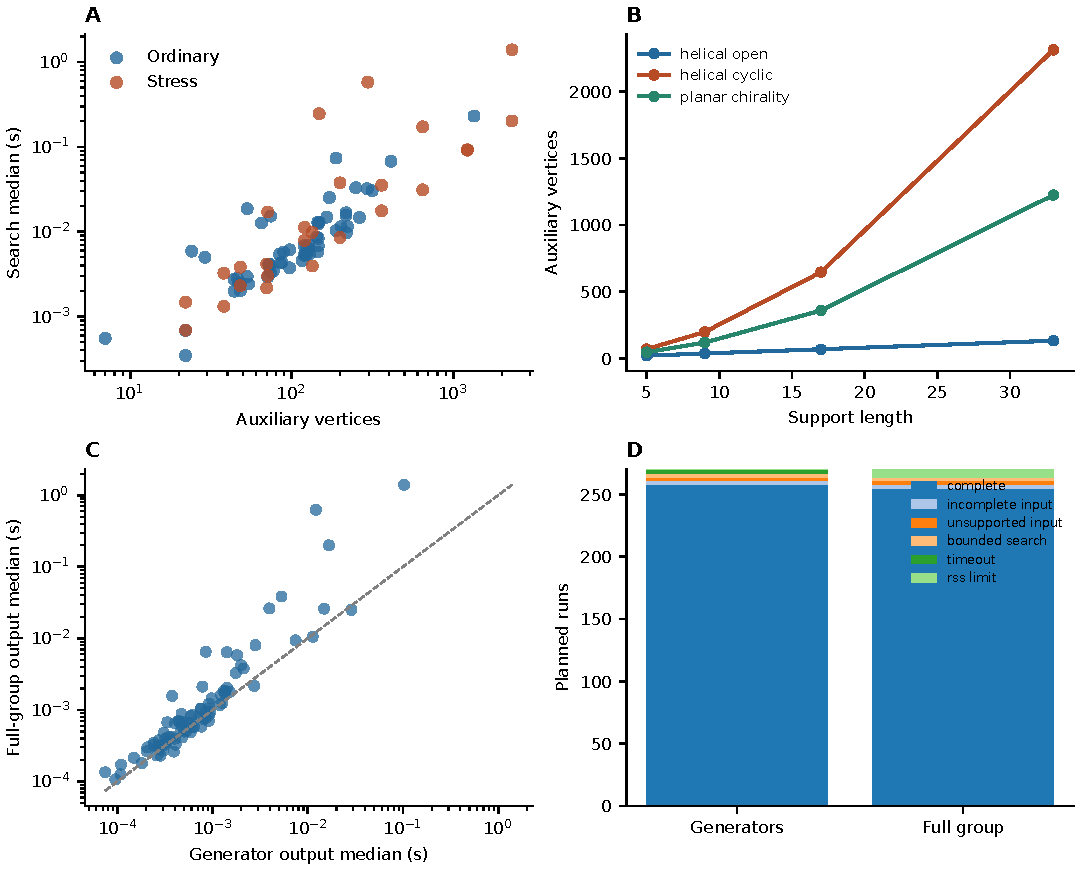
\includegraphics[width=0.98\textwidth]{fig/controlled_stereo_costs.pdf}
\caption{Controlled configured-graph costs. (A) Generator-mode search medians
against expansion size for completed cases. (B) Variable-support expansion
size. (C) Witness-output medians on inputs completed by both modes; the dashed
line indicates equality. (D) All planned trial outcomes. Each input has three
repetitions; the plot and timings do not treat censored trials as completed.
Different completion sets preclude interpreting pooled mode medians as a
matched speed comparison.}
\label{fig:controlled-costs}
\end{figure*}

\subsection{Registration demonstration}
\label{sec:registration}

Independently labelled collections mix duplicates under proper frame moves
and renumbering with distinct stereoisomers across six conventional frame
families. At sizes 8, 16, 32, 64 and 128, each pipeline is executed three times
with alternating order. Pairwise grouping compares records with existing group
representatives; certificate grouping computes one full certificate per record
and uses a digest index followed by exact byte equality. Both include input
preparation and grouping/storage costs. All 30 pipelines recover the complete
expected partitions. Separate chemical/Lewis/ACS profile checks and strict
partial-input refusal pass.

Figure~\ref{fig:registration-costs} shows no runtime crossover in this tested
range. At 128 records, pairwise and certificate medians are respectively
\pgfmathprintnumber[fixed,precision=3,zerofill]{\RegistrationOneTwentyEightPairwiseMedian}\,s
and
\pgfmathprintnumber[fixed,precision=3,zerofill]{\RegistrationOneTwentyEightCertificatesMedian}\,s.
This small curated from-scratch workload supports registration correctness,
not an acceleration claim or a chemical holdout claim. Memory is measured for
the whole study rather than isolated pipelines, and background host load limits
timing generalization. Persistent-index query workloads remain unmeasured.

\begin{figure*}[htbp]
\centering
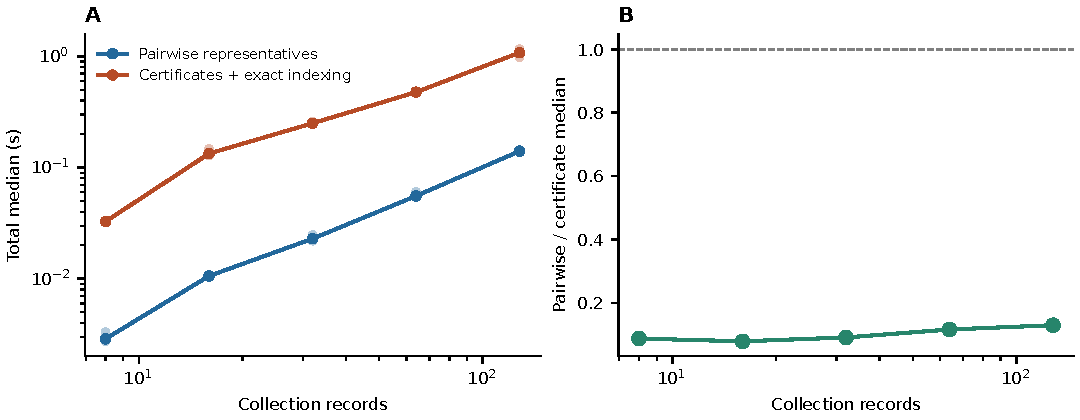
\includegraphics[width=0.98\textwidth]{fig/curated_stereo_registration.pdf}
\caption{Curated registration workload. (A) Total medians and individual
repetitions for both pipelines. (B) Pairwise/certificate median ratio; values
below one favour pairwise grouping. Both methods recover the independently
specified groups, but certificate grouping is slower at every tested size.}
\label{fig:registration-costs}
\end{figure*}

\subsection{New chemical examples and structural adjudication}
\label{sec:chemical-results}

We froze source selection and annotation before production evaluation.
The new coordination inputs are initial generated geometries from the MACE
archive \cite{pidko2024macedata}, distributed under CC~BY~4.0. They cover
\ChemicalCoordinationConstitutions{} Mn/Ru constitutions absent from the
development corpora. Source donor isotopes encode coordination slots and are
removed from physical isotope identity; supplied local tetrahedral frames are
retained. An independent proper-rotation/reflection fit, followed by direct
assignment-partition enumeration, supplies the reference. The frozen fit
criteria certify \ChemicalCoordinationCertified/\ChemicalCoordinationSelected{}
geometries and refuse \ChemicalCoordinationUnresolved{} distorted examples;
these refusals receive no production score.

All certified source and coordinate-reflected states agree with production
mirrors and reverse renumbering in \ChemicalCoordinationCodeComputations{}
full-certificate computations. The observed \ChemicalCoordinationObservedSourceMirrorClasses{}
source/mirror classes reproduce both directions of reference equality.
Complete independent references contain \ChemicalCoordinationReferenceAssignments{}
formal assignments and \ChemicalCoordinationReferenceClasses{} classes across
the selected constitutions; production coding covers the certified source/mirror
states, rather than all reference assignments (Table~\ref{tab:chemical-evidence}).
The source geometries do not establish experimental isolation or stability.

Separately, \ChemicalNegativeSelected{} new PubChem-sourced biaryl constitutions
carry independently verified full typed automorphisms that fix each axis and
exchange a terminal ligand pair. Original and reverse-renumbered perception
agree with every negative witness. These are constitutional specificity
controls, with no barrier or persistence annotation.

The RotA review fixes \ChemicalRotASelected{} historical additional loci across
\ChemicalRotAStrata{} strata and \ChemicalRotASourceRecords{} source molecules.
Algorithm confirmation/rejection status is withheld during annotation, but
source supports and categories assist the review; it is development-corpus
adjudication. Complete per-case partitions, mirror maps and renumberings agree
over \ChemicalRotAFormalAssignments{} assignments in
\ChemicalRotACodeComputations{} certificate computations. Of the
\ChemicalRotAAxisSupports{} axis supports, \ChemicalRotAOrdinarySingleBondAxes{}
are ordinary single bonds and \ChemicalRotAAromaticAxes{} are aromatic edges.
The latter are conditional configuration-model tests, with no claim of
ordinary single-bond atropisomerism. The remaining loci are
\ChemicalRotATetrahedralPairs{} atom pairs and \ChemicalRotASpiroCenters{}
spiro centers. Category-specific perception is checked separately from global
configured identity; terminal ligand equivalence can coexist with distinct
coupled configurations. All studies use automated independent mathematical
annotation, rather than an independent human chemical review.

\begin{table}[htbp]
\caption{Chemical evidence and its evaluated population. Reference classes
are reported per constitution or case; counts are never pooled as chemical accuracy.}
\label{tab:chemical-evidence}
\centering
\small
\begin{tabularx}{\textwidth}{@{}lrrX@{}}
\toprule
Protocol & Selected & Complete & Truth and evaluated scope \\
\midrule
Coordination & \ChemicalCoordinationSelected & \ChemicalCoordinationCertified
 & Independent geometry and partitions; source/mirror states only;
 \ChemicalCoordinationUnresolved{} geometry refusals \\
Sourced negatives & \ChemicalNegativeSelected & \ChemicalNegativePassed
 & Full typed axis-fixed symmetry; \ChemicalNegativePerceptionComputations{}
 original/renumbered perception calls \\
RotA review & \ChemicalRotASelected & \ChemicalRotAComplete
 & \ChemicalRotAFormalAssignments{} assignments;
 \ChemicalRotASumPerCaseClasses{} classes summed per case;
 \ChemicalRotAPerceptionComputations{} perception calls \\
\bottomrule
\end{tabularx}
\end{table}

\subsection{Perception and derived naming}
\label{sec:perception-results}

Table~\ref{tab:perception-results} separates configuration-neutral carrier
recovery from downstream naming.  Retaining oriented frames at neighboring
elements recovers every annotated locus.  Erasing all configuration leaves
\AllErasedMisses{} unresolved carbon tetrahedral positions whose center stabilizer contains
an odd slot permutation.  Every one is recovered in the retained setting,
showing that the deficit is orientation-dependent ligand distinction rather
than unsupported carrier topology.

\begin{table}[htbp]
\caption{Broad typed-carrier recovery in two settings.}
\label{tab:perception-results}
\centering
\begin{tabularx}{\textwidth}{@{}Xrrr@{}}
\toprule
Task & Retained & Erased & Reference \\
\midrule
ACS configured source loci & \AcsRetainedRecovered & \AcsErasedRecovered & \AcsErasedReferenceLoci \\
CIP local positions & \CipRetainedRecovered & \CipErasedRecovered & \CipErasedReferenceLoci \\
\quad tetrahedral & \CipTetrahedralRetainedRecovered & \CipTetrahedralErasedRecovered & \CipTetrahedralErasedReference \\
\quad planar & \CipPlanarRetainedRecovered & \CipPlanarErasedRecovered & \CipPlanarErasedReference \\
\quad axial/helical & \CipAxialRetainedRecovered & \CipAxialErasedRecovered & \CipAxialErasedReference \\
RotA typed loci & \RotARetainedRecovered & \RotAErasedRecovered & \RotAErasedReferenceLoci \\
RotA cumulene paths & \RotAExpandedRetainedRecovered & \RotAExpandedErasedRecovered & \RotAExpandedErasedReference \\
Reverse-renumbered records & \DevelopmentRows & \DevelopmentRows & \DevelopmentRows \\
\bottomrule
\end{tabularx}
\end{table}

The ACS and CIP erased misses number \AcsErasedMisses{} and \CipErasedMisses{}, respectively, and are all
carbon tetrahedral carriers classified as symmetry related under the exact
configuration-erased stabilizer.  Axis recovery asserts typed candidate
topology, not handedness or configurational stability.  Additional candidate
inventories are retained per record but are not presented as specificity
scores where negative truth is absent.
We therefore add a separate \SyntheticAxisNegatives-case synthetic negative protocol:
\SyntheticAxisWitnessNegatives{} axis-like constitutions are rejected by explicit axis-fixed automorphisms
that exchange a terminal ligand pair, and \SyntheticAxisNoSupportNegatives{} contain no supported axis
topology. All cases pass reverse atom renumbering and none is a confirmed-axis
false positive.  This protocol establishes constitutional specificity only;
it supplies no experimental barrier, stability, or handedness truth.

With the pinned three-dimensional orientation input and supplied family
categories selecting the projections, the CIP evaluator is exact on
\CipCoordinatesExactRecords/\CipCoordinatesRecords{} records and recovers
\CipCoordinatesCorrectLabels/\CipCoordinatesExpectedLabels{} reference labels
while emitting \CipCoordinatesEmittedLabels{} (73.96\% recall, 98.83\%
precision). It emits \CipCoordinatesWrongLabels{} wrong labels and misses
\CipCoordinatesMissingLabels{}. The SMILES-only baseline remains
\CipSmilesExactRecords/\CipSmilesRecords. Reviewed primary limitations among the 113 non-exact
records are 83 ranking defects, 21 missing configured orientations, and 9
unsupported classes.  The implementation includes Rules 1a/1b/2, simple mancude-ring
averaging, Rule 3, and the reference-independent one-pair subset of Rules
4c/5; multi-unit Rule 4b remains fail-closed.  These naming results do not participate
in any canonical certificate.
Moreover, complete assignment is not identifiable from the supplied SMILES contract:
VS010 and VS011 have byte-identical input and mutually opposite helical label
sets.  Thus any deterministic SMILES-only method has an upper bound of
299 exact records.  The pinned three-dimensional file resolves this
input obstruction: the pair has opposite signs under the same
translation- and proper-rotation-invariant oriented-volume witness.
The coordinates distinguish this otherwise identical-input pair. They complete
2/2 helical and 5/5 CT4 records, while unambiguous transport completes 4/7 AT
records. The remaining sequence rules, three ambiguous AT transports, and
TH3/TH5 projection remain algorithmic future work.

\subsection{Molecular chirality}
\label{sec:chirality-results}

The ACS results expose three distinct protocols (Table~
\ref{tab:chirality-results}).  The specialized topology-completion classifier
reproduces all 258 manual labels, matching the published \stereomolgraph result.
It uses provisional probes and the publisher-compatible identity convention.
The exact-stereograph row instead measures the configured certificate currently
implemented and must not inherit the 258/258 score.

\begin{table}[htbp]
\caption{Whole-molecule chirality on 258 ACS records.  ``Agreement'' compares
the declared procedure with the ACS topology labels; the exact-stereograph
cross-profile differences are not internal certificate errors.}
\label{tab:chirality-results}
\centering
\begin{tabularx}{\textwidth}{@{}XrrX@{}}
\toprule
Procedure & Agreement & Fraction & Boundary \\
\midrule
Topology completion (this work) & \AcsTopologyCorrect/\AcsSourceRecords & 1.000 & ACS-specialized probes \\
Exact + necessary global certificate & \AcsGlobalCorrect/\AcsSourceRecords & 0.996 & 30\,s budget; orientation unspecified \\
\stereomolgraph (published) & 258/258 & 1.000 & Published comparator \\
\stereomolgraph (pinned live replay) & \AcsLiveSmgCorrect/\AcsSourceRecords & 0.984 & Separate release/environment replay \\
InChI (published) & 238/258 & 0.922 & Published comparator \\
\rdkit{} SMILES (published) & 235/258 & 0.911 & Published comparator \\
chython (published) & 210/258 & 0.814 & Published comparator \\
Exact supplied stereograph & \AcsSourceCorrect/\AcsSourceRecords & 0.981 & \AcsSourceDefinitive{} definitive; 5\,s budget \\
\bottomrule
\end{tabularx}
\end{table}

Under the 5\,s budget, the supplied-configuration path gives
\AcsSourceDefinitive{} definitive outcomes and \AcsSourceCorrect{} agreements
among \AcsSourceRecords{} inputs. VS126, VS127 and VS208 time out. Accuracy among
definitive outcomes is \AcsSourceCorrect/\AcsSourceDefinitive; correct decisions
over all inputs are \AcsSourceCorrect/\AcsSourceRecords.
Figure~\ref{fig:exact-mirror-mismatches} shows the two remaining definitive
task-boundary differences, VS170 and VS300. The corrected VS215
and VS216 resonance regressions are concordant achiral cases and are therefore
omitted from the figure.  Chemical mirror identity compares the exact
resonance family while preserving genuine bond-order differences. VS170
remains chiral because its
literal \code{S-I} and \code{S\#I} ligands are distinct; the ACS topology profile omits
that distinction. VS300 is exactly achiral for the represented
configured support: its mirror map fixes the central configured atom and
exchanges the two configured cage centers.  The ACS topology-completion
protocol adds global probes and therefore reaches its chiral label under a
different support boundary. Neither difference is a search or certificate
failure. Strict single-Lewis-state and ACS connectivity-only identities remain
available as explicit profiles, and the strict library mode that audits
undeclared supported loci remains separate from this supplied-configuration
benchmark.

The new coupled-frame representation makes the VS300 distinction executable
without rewriting the source tags.  Its map-independent global certificate
proves necessary chirality for sanitized VS300 topology but retains
orientation as unspecified.  Combining this proof with the unchanged exact
source-declared procedure gives the separately named
\AcsGlobalCorrect/\AcsSourceRecords{} protocol under a 30\,s budget; VS170
remains the sole disagreement because chemical identity intentionally retains
its bond-order distinction.  This later result does not overwrite the frozen
historical 256/258 artifact. Its stronger time budget must not be transferred
to the five-second source-declared row. The comparator replays at pinned commit \code{2189f61} and current
commit \code{2b99f62} each agree with the manual column on
\CurrentSMGCorrect/\AcsSourceRecords{} rows. Their four disagreements are
VS246, VS247, VS248 and VS299, separate from the published 258/258 column.
A matched-inventory diagnostic transfers every upstream configured descriptor
losslessly, including typed lone pairs, into the generic SynKit canonizer.
Both algorithms then give the same mirror verdict on all four inputs. Removing
the represented planar-bond descriptors changes both verdicts to achiral.
An unrefined upstream stereo-map search also agrees with its fingerprint-
assisted comparison. Thus the four-row discrepancy concerns the adapters'
represented information, not evidence that canonicalization outperforms the
upstream graph matcher. The ablation changes the configured object; it does
not adjudicate the preferred chemical convention.

\begin{figure*}[htbp]
\centering
\resizebox{0.98\textwidth}{!}{% The two declared task-boundary differences, stated as certificate tests.
% Each panel pairs the rendered structure with the two contracts that disagree
% and with the mirror-certificate comparison that decides the exact verdict.
% Requires concept_style.tex; libraries arrows.meta, calc, backgrounds.
\begin{tikzpicture}[
  font=\small,
  chip/.style={rounded corners=2pt, line width=0.5pt, font=\scriptsize,
    inner xsep=3.6pt, inner ysep=2.4pt},
  acs/.style={chip, draw=black!32, fill=black!2, text=black!62},
  chiral/.style={chip, draw=ioBlue!60!black, fill=ioBlue!8,
    text=ioBlue!42!black, font=\scriptsize\bfseries},
  achiral/.style={chip, draw=ioGreen!62!black, fill=ioGreen!10,
    text=ioGreen!42!black, font=\scriptsize\bfseries},
  crit/.style={font=\scriptsize, text=black!70},
  why/.style={font=\scriptsize, text=black!58, align=center,
    text width=6.25cm, inner sep=0pt},
]

% ------------------------------- A: VS170 --------------------------------
\begin{scope}
  \filldraw[iopanel] (-7.25,-0.78) rectangle (-0.15,5.60);
  \node at (-3.70,2.75)
    {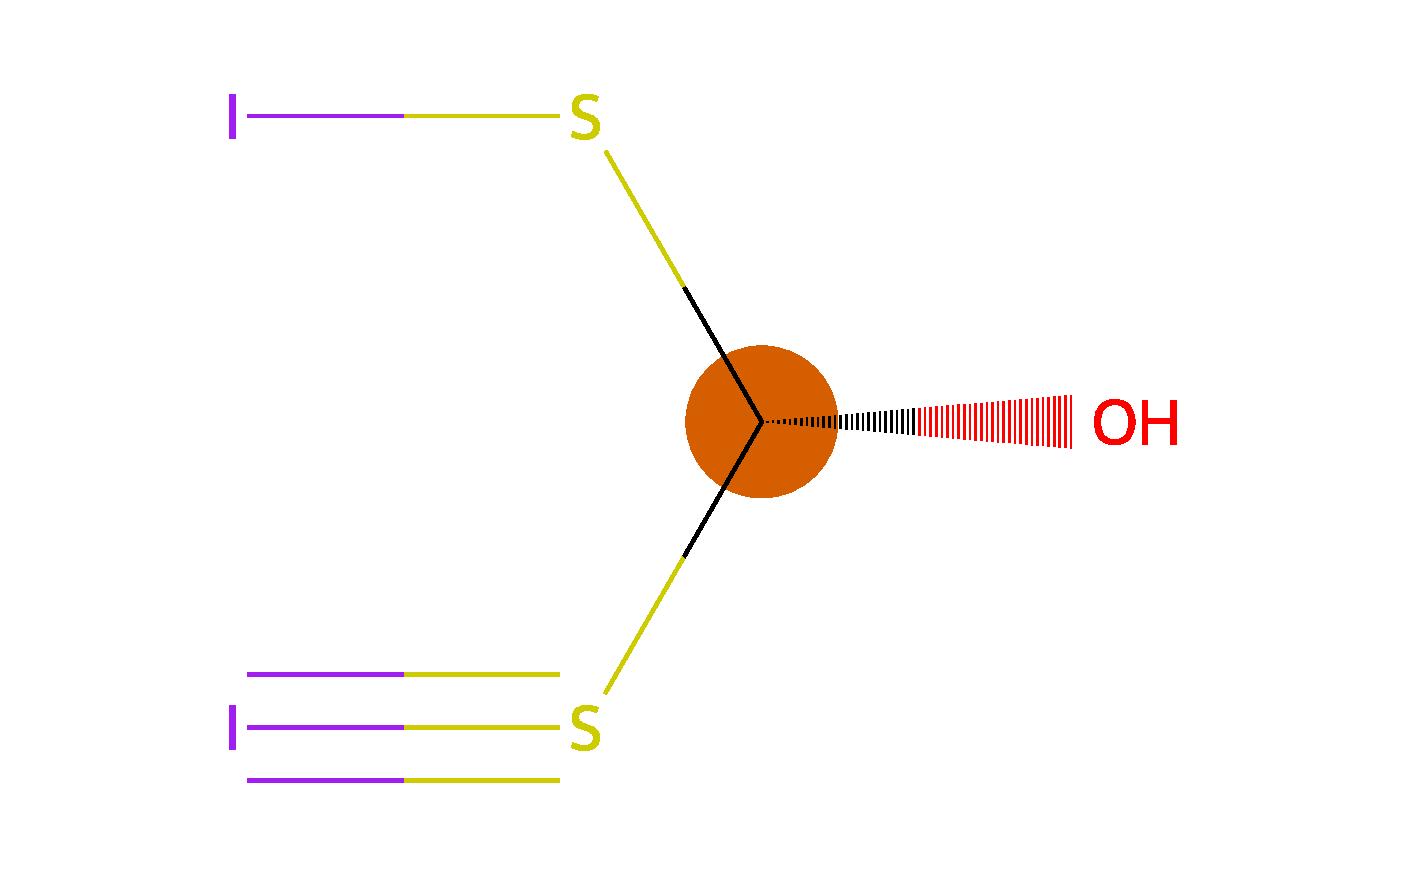
\includegraphics[width=6.0cm]{fig/exact_mirror_vs170.pdf}};
  \iosub{-6.92,5.26}{A}{VS170}
  \node[acs,     anchor=east] at (-3.85,0.55) {ACS topology: achiral};
  \node[chiral,  anchor=west] at (-3.55,0.55) {exact: chiral};
  \node[crit] at (-3.70,0.05)
    {\(C_{\mathrm{SG}}(\mathcal X)\neq C_{\mathrm{SG}}(\mu\mathcal X)\)};
  \node[why] at (-3.70,-0.43)
    {\(\mathrm{S{-}I}\) and \(\mathrm{S{\equiv}I}\) stay distinct};
\end{scope}

% ------------------------------- D: VS300 --------------------------------
\begin{scope}
  \filldraw[iopanel] (0.15,-0.78) rectangle (7.25,5.60);
  \node at (3.70,2.75)
    {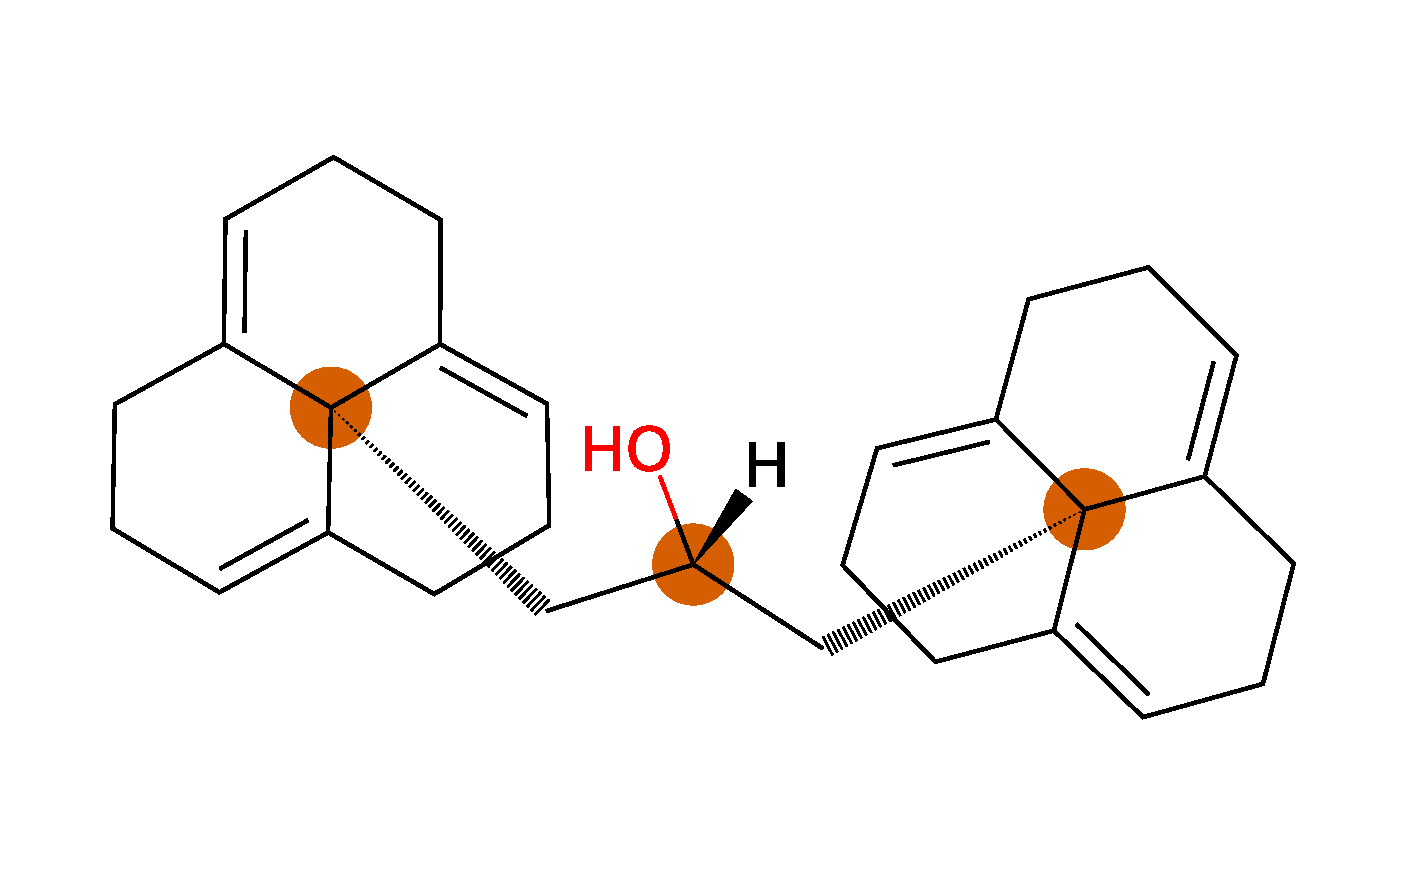
\includegraphics[width=6.0cm]{fig/exact_mirror_vs300.pdf}};
  \iosub{0.48,5.26}{D}{VS300}
  \node[acs,     anchor=east] at (3.55,0.55) {ACS topology: chiral};
  \node[achiral, anchor=west] at (3.85,0.55) {exact: achiral};
  \node[crit] at (3.70,0.05)
    {\(C_{\mathrm{SG}}(\mathcal X)=C_{\mathrm{SG}}(\mu\mathcal X)\)};
  \node[why] at (3.70,-0.43)
    {\(\mu\) fixes the center, exchanges the cages};
\end{scope}
\end{tikzpicture}
}
\caption{The two remaining declared task-boundary differences in the
258-record source-declared-configuration audit. Orange circles mark atoms carrying
explicit source \code{@}/\code{@@} configurations; wedge/hash bonds show the
corresponding local orientation. In A, chemical identity preserves the genuine
\(\mathrm{S{-}I}/\mathrm{S{\equiv}I}\) distinction and returns chiral, whereas
the ACS connectivity-only profile returns achiral. In D, the exact mirror
isomorphism fixes the central configured carbon and exchanges the two
configured cages, so the represented local configurations compensate in a
meso-like, mirror-fixed arrangement.  This is not a general meso assignment:
the historical source-declared protocol lacks the coupled relation.  The
separate global certificate encodes the topology-completion probes as one
orientation-unspecified framework and proves the ACS chiral outcome without
reinterpreting the three source tags.}
\label{fig:exact-mirror-mismatches}
\end{figure*}

After stereo removal, the 258 records reduce to 214 unique constitutions.
Completion assessment returns 125 necessarily chiral, 66 necessarily achiral,
and 67 configuration dependent, with no unsupported/incomplete row; all 258
rows are definitive.  VS226 is settled by actual exhaustion of six
symmetry-unique isomers.  Automorphism-parity constraints prove that VS265 and
VS266 have no achiral completion and construct an achiral completion of VS268.
The erased manual label remains among the possible configurations for all 258
rows.  This is a coverage statement, not recovery of information that was
removed.

\section{Discussion}
\label{sec:conclusion}

\subsection{Principal findings}

Faithful reduction resolves simultaneous configurations and global symmetry
within a declared identity profile. It preserves the distinction between
\(E/Z\) and mirror relations and recognizes mirror-fixed \emph{meso}
structures without counting local labels. Formal assignments are products of
local orbits; global classes are their orbits under constitutional
automorphisms. Corollary~\ref{cor:raw-formal-global} justifies formal
enumeration, and the retained raw encodings check its implementation.
Independent partition and chemical studies support these declared contracts;
perception, naming and performance results remain separate evidence.

\subsection{Limitations}

The method records assigned relative stereochemistry; it does not infer
three-dimensional configuration, conformational populations, reaction
selectivity, or configurational stability.  Axis detection therefore does not
establish that an atropisomer is isolable.  Global/topological support is
implemented for coupled tetrahedral frame certificates; additional framework
geometries and automatic configured-orientation perception remain unsupported.
The exact analyzer also fails closed above 256 support atoms or 64 coupled
frames, and for frames distributed over disconnected components.
Enhanced-stereo population semantics also remain unsupported.

The exact certificate consumes all ten configured families, but legacy
value identity, rule matching, JSON/GML interchange, and the \rdkit adapter
still expose narrower class sets. Exact canonicalization materializes complete
local orbits and uses verified automorphism pruning. Bounded correctness
checks do not establish canonical-SMILES-scale performance; the controlled
cost study explicitly retains resource-censored outcomes. Raw B is now
complete, but raw C is represented only by the complete VS146 slice; the
other eight raw C Cartesian products remain unexecuted and are not needed for
the exact formal quotient.  The CIP kernel implements
Rules~1a, 1b, and 2, simple mancude averaging, Rule~3, and the
reference-independent one-pair subset of Rules~4c/5; multi-unit Rule~4b and
coordination-geometry projection remain fail-closed.  Finally, ACS, RotA, and
CIP provide different kinds of truth and cannot support one pooled accuracy
statistic.

\subsection{Future work}

Priorities are sparse certificate construction and component decomposition,
additional framework geometries and enhanced-stereo population semantics,
and migration of extended carriers into legacy interchange surfaces.
Experimental axis stability and handedness need separately sourced truth.
Multi-unit CIP Rule~4b, hierarchical ring digraphs and coordinate-based
orientation projections can improve naming coverage without changing identity.

\section{Conclusions}

The configured stereograph, rather than a collection of local names, is the
appropriate identity object for molecular stereochemistry.  The faithful
auxiliary-graph expansion and complete canonical certificate decide global
stereo-isomorphism exactly; the geometry-specific mirror action then makes
whole-molecule chirality a theorem-backed consequence.  Potential-carrier
perception remains configuration neutral, authorized evidence is attached
through a typed boundary, and incomplete chemistry fails closed.  Finding a
possible stereocenter is therefore only the first step and never, by itself,
establishes molecular chirality.

\section*{Abbreviations}
ACS, American Chemical Society; API, application programming interface;
CC~BY, Creative Commons Attribution; CC~BY-NC, Creative Commons Attribution
NonCommercial; CIP, Cahn--Ingold--Prelog; CPU, central processing unit;
GML, Graph Modelling Language; ITS, imaginary transition state;
JSON, JavaScript Object Notation; LLG, Lewis-labeled graph;
RMSD, root-mean-square deviation; RSS, resident set size;
SMILES, simplified molecular-input line-entry system;
SP, square-planar; TBP, trigonal-bipyramidal; OH, octahedral.

\section*{Declarations}

\subsection*{Ethics approval and consent to participate}
Not applicable.

\subsection*{Consent for publication}
Not applicable.

\subsection*{Availability of data and materials}
The project is \synkit, with source code under the MIT License at its
project home page \cite{synkitSource}. General project documentation
\cite{synkitDocumentation} and archived project releases
\cite{synkitProjectArchive} are publicly available; those releases do not
identify the exact experimental revision described here. The ACS validation set is
redistributed under CC~BY-NC~4.0 and RotA under the MIT License. The original
CIP publisher supporting archive, prepared SMILES and original coordinates
are included under CC~BY-NC~4.0 with attribution \cite{hanson2018cip};
the license is separate from the software license. The later amended GitHub
coordinate file is external and separately identified for historical replay.
The selected MACE geometries and their attribution are
included under CC~BY~4.0 \cite{pidko2024macedata}; sourced negative inputs,
retrieval responses, frozen annotations and production reports accompany the
revision. The research checkout and package metadata report \synkit
\code{1.6.2}. Exact source commits and input checksums identify the revision;
the package version alone does not identify the experimental code. The release
material includes a Linux x86\_64/Python 3.12.12 wheel-hash environment lock
and the original conda bootstrap specification. The implementation is in
Python; the tested environment uses RDKit 2026.03.1 and NetworkX 3.6.1,
with a C++ compiler for the native comparator. The software has no additional
restriction on use by non-academics; the separately licensed source datasets
retain their stated terms. An exact review archive is provided locally with
a source-commit identifier and SHA-256 inventory; this review version has no
public archive DOI.

\subsection*{Additional files}
Additional file 1: \code{Additional\_file\_1.pdf} (PDF).
\emph{Supporting information: Exact canonicalization of configured molecular
stereographs}. This file contains the technical algebra and proofs,
representation and API contracts, benchmark protocols, chemical annotation
details, resource measurements and reproduction instructions. It supplements
the main article; machine-readable inputs, reports and software are retained
in the separately identified research archive.

\subsection*{Competing interests}
The authors' declaration of competing interests is pending.

\subsection*{Funding}
This work has received funding from the European Union’s Horizon Europe
Doctoral Network programme under the Marie Sk{\l}odowska-Curie grant
agreement No. 101072930 (TACsy---Training Alliance for Computational
systems chemistry).  Views and opinions expressed are however those of the
author(s) only and do not necessarily reflect those of the European
Union. Neither the European Union nor the granting authority can be held
responsible for them.

Further support was provided by the Novo Nordisk Foundation under grant
reference NNF21OC0066551 (Mathematical Modelling for Microbial Community
Induced Metabolic Diseases, MATOMIC).

PFS acknowledges support by the Federal Ministry of Research, Technology,
and Space of Germany through DAAD project 57616814 (SECAI, School of
Embedded Composite AI), jointly with S{\"a}chsische Staatsministerium für
Wissenschaft, Kultur und Tourismus in the programme Center of Excellence
for AI-research \emph{Center for Scalable Data Analytics and Artificial
Intelligence Dresden/Leipzig} (ScaDS.AI, proj.\ no.\ SCADS24B), and by the
Deutsche Forschungsgemeinschaft (DFG, German Research Foundation) under
Germany's Excellence Strategy (EXC-3105/1, 533765739).

\subsection*{Author contributions}
T.-L.P. conceived and developed the method, implemented the reference
realization, designed and performed the validation, prepared the figures, and
wrote the manuscript.
P.F.S. and D.M. revised the manuscript, supervised the project, and secured
funding.

\subsection*{Acknowledgements}
\synkit builds on \rdkit and \networkx.  The relative-stereo descriptor model
was cross-validated against the MIT-licensed \stereomolgraph implementation;
its notice and pinned conformance commit are distributed with the source.

\clearpage
\bibliography{references}

\clearpage
\appendix
% Detailed algebra and boundary contracts moved from the main narrative.
% Labels are retained so all proof dependencies remain explicit.
\section{Detailed local algebra and information boundaries}
\label{sec:detailed-algebra}

\subsection{Frame action and unique alignments}
\begin{lemma}[Frame action]
\label{lem:frame-action}
Let \(u\) be a frame of length \(k\), let \(p,q\in S_k\), and let \(r\) be an
injective relabeling of references.  Then
\[
  \operatorname{id}\cdot u=u,
  \qquad
  p\cdot(q\cdot u)=(q\circ p)\cdot u
  =(q\mathbin{\mathrm{then}}p)\cdot u,
  \qquad
  r(p\cdot u)=p\cdot(ru).
\]
Hence Eq.~\eqref{eq:action} is a right action of \(S_k\) on frames, the orbit
\([u]_\Gamma=\{\gamma\cdot u:\gamma\in\Gamma\}\) is well defined for every
subgroup \(\Gamma\leq S_k\), and two witnesses are sequenced by
\(p\mathbin{\mathrm{then}}q\):
\((p\mathbin{\mathrm{then}}q)\cdot u=q\cdot(p\cdot u)\).
\end{lemma}

\begin{proof}
Coordinatewise,
\((p\cdot(q\cdot u))_i=(q\cdot u)_{p(i)}=u_{q(p(i))}=((q\circ p)\cdot u)_i\),
which is the stated anti-homomorphism law and is exactly the convention
\(p\mathbin{\mathrm{then}}q=p\circ q\) of the slot images.  Thus the
\code{then} API sequences tuple reorderings, although slot-map composition
has the reverse order from composition of those reorderings.  A relabeling acts on the values held by
the slots and the group acts on the slots themselves, so
\((r(p\cdot u))_i=r(u_{p(i)})=(ru)_{p(i)}=(p\cdot(ru))_i\).  Injectivity of
\(p\cdot u\) and of \(ru\) is inherited from \(u\) and \(r\).
\end{proof}

\begin{lemma}[Unique alignment]
\label{lem:unique-alignment}
Let \(u\) and \(v\) be frames of length \(k\) with
\(\operatorname{im}u=\operatorname{im}v\).  Then there is exactly one
\(\rho\in S_k\) with \(v=\rho\cdot u\), namely \(\rho=u^{-1}\circ v\).  In
particular every subgroup \(\Gamma\leq S_k\) acts freely on frames, so all
orbits have cardinality \(|\Gamma|\).
\end{lemma}

\begin{proof}
Both tuples are bijections onto the same image, so \(\rho=u^{-1}\circ v\) is a
permutation of slots and \((\rho\cdot u)_i=u_{\rho(i)}=v_i\).  If
\(v=\rho'\cdot u\) as well, then \(u_{\rho(i)}=u_{\rho'(i)}\) for every \(i\),
and injectivity of \(u\) forces \(\rho=\rho'\).  Freeness is the case
\(v=u\), which yields \(\rho=\operatorname{id}\), and the orbit--stabilizer
theorem then gives \(|[u]_\Gamma|=|\Gamma|\).
\end{proof}

The tetrahedral case is the smallest instance of this local state model.  Four
distinct ligand references admit \(4!=24\) frames, on which \(S_4\) acts freely
and transitively; the subgroup \(A_4\) has index two, so the frames split into
two orbits of twelve.  Even permutations are rigid rotations of one local
configuration and odd permutations reach the mirror orbit.

\begin{proposition}[Local parity criterion]
\label{prop:local-parity}
Let \(u\) and \(v\) be tetrahedral frames with
\(\operatorname{im}u=\operatorname{im}v\), and let \(\rho\in S_4\) be the unique
alignment of Lemma~\ref{lem:unique-alignment}, \(v=\rho\cdot u\).  Then
\[
 [u]_{A_4}=[v]_{A_4}
 \quad\Longleftrightarrow\quad
 \operatorname{sgn}(\rho)=+1 .
\]
If \(\operatorname{sgn}(\rho)=-1\), the two frames lie in the two distinct
cosets of \(A_4\) in \(S_4\).
\end{proposition}

\begin{proof}
By Lemma~\ref{lem:unique-alignment} the alignment \(\rho\) exists and is unique,
so \([u]_{A_4}=[v]_{A_4}\) holds precisely when \(\rho\in A_4\).  The sign
homomorphism \(\operatorname{sgn}:S_4\to\{\pm1\}\) has kernel \(A_4\), whence
\(\rho\in A_4\) is equivalent to \(\operatorname{sgn}(\rho)=+1\).  Since
\([S_4:A_4]=2\), every odd alignment lies in the unique remaining coset and
therefore reaches the opposite orbit.
\end{proof}


\subsection{Focal-configuration-neutral carrier perception}
\label{sec:perception-algorithm}

Perception produces typed \emph{potential} elements, not configured
descriptors.  Let \(\mathcal F\) be an optional set of supplied oriented frames
at other loci.  The focal frame is removed before its carrier is assessed, and
all CIP properties, coordinates, canonical local descriptors, and atom indices
are excluded.  Algorithm~\ref{alg:perception} makes this boundary explicit.

\begin{definition}[Potential-carrier predicate]
\label{def:potential-carrier}
For a family policy \(P\), identity profile \(\chi\), type \(\tau\), and
candidate support \(s\), let
\[
  \operatorname{Pot}_{\tau,P}(G_\chi,s;\mathcal F_{-s})
\]
mean that \(s\) is a structurally valid support of type \(\tau\) and passes
the registered configuration-neutral feasibility test.  The returned evidence
record is
\[
  e_s=(s,\tau,A_s,q_s,r_s,\bot,\textsc{unassessed}),
\]
where \(A_s\) is the action induced by the support stabilizer
\(\operatorname{Aut}_\chi(G,\mathcal F_{-s})_s\), \(q_s\) is the potential-carrier status,
\(r_s\) is its reason, \(\bot\) denotes absent configuration, and the final
field records that configurational persistence has not been assessed.
\end{definition}

The predicate is deliberately an over-approximation of experimentally
persistent stereochemistry.  It asserts neither a handedness nor a molecular
chirality verdict.  Its mathematical requirement is equivariance: if
\(f\in\operatorname{Iso}_\chi(G,H)\), then
\begin{equation}
  \operatorname{Pot}_{\tau,P}(G_\chi,s;\mathcal F_{-s})
  \Longleftrightarrow
  \operatorname{Pot}_{\tau,P}(H_\chi,f(s);f\mathcal F_{-s}),
  \qquad
  f_*A_sf_*^{-1}=A_{f(s)} .
  \label{eq:perception-equivariance}
\end{equation}

\begin{algorithm}[htbp]
\caption{Focal-configuration-neutral stereo-carrier perception}
\label{alg:perception}
\begin{algorithmic}[1]
\Require LLG \(G\), identity profile \(\chi\), optional neighboring frames \(\mathcal F\), family policy \(P\)
\Ensure Equivariant potential-element evidence with no focal configuration; serialization order is not identity
\State \(G_0 \gets \Call{EraseDerivedAndConfiguredState}{G_\chi}\)
\State \(\mathcal C \gets \Call{EnumerateTypedSupports}{G_0,P}\)
\State \(\mathcal E \gets [\,]\)
\ForAll{\(s\in\Call{CanonicalSupportOrder}{\mathcal C}\)}
  \If{\(\neg\Call{ValidateSupport}{G_0,s}\)}
    \State \(\mathcal E\gets\mathcal E\mathbin{\|}(s,\textsc{rejected},\textsc{invalid support})\)
    \State \textbf{continue}
  \EndIf
  \State \(\mathcal F_{-s}\gets\Call{RemoveFocalFrame}{\mathcal F,s}\)
  \State \(G_s\gets\Call{AddNeighborFrameConstraints}{G_0,\mathcal F_{-s}}\)
  \State \(A_s\gets\Call{InducedStabilizerAction}{\operatorname{Aut}(G_s)_s}\)
  \State \((q,r)\gets\Call{ConfirmCarrier}{\operatorname{type}(s),G_s,s,A_s}\)
  \State \(\mathcal E\gets\mathcal E\mathbin{\|}(s,q,r,\bot,\textsc{unassessed})\)
\EndFor
\State \Return \(\mathcal E\)
\end{algorithmic}
\end{algorithm}

\begin{proposition}[Perception soundness]
\label{prop:perception-soundness}
Assume every registered support enumerator, validator, and family confirmation
test is invariant under \(\chi\)-isomorphism transporting the supplied
neighboring frame constraints. Algorithm~\ref{alg:perception}
is then equivariant in the sense of Eq.~\eqref{eq:perception-equivariance}.
Its output contains no configuration that could depend on atom numbering,
CIP priority, or the focal input orientation.
\end{proposition}

\begin{proof}
Support enumeration and validation commute with \(f\) by assumption.
Conjugation by \(f\) maps
\(\operatorname{Aut}_\chi(G_s)_s\) onto
\(\operatorname{Aut}_\chi(H_{f(s)})_{f(s)}\), hence maps the induced slot
action and every invariant confirmation result onto its counterpart.
Canonical support ordering changes only output order.  The focal orientation
and all derived naming data were erased, and the algorithm writes \(\bot\) in
every configuration field.
\end{proof}

\(\Call{ConfirmCarrier}{}\) is geometry specific.  A tetrahedral support is
confirmed exactly when its center-stabilizer action contains no odd
permutation of the four coordination slots.  Planar-bond and axis candidates
require non-exchangeable terminal reference pairs under the support
stabilizer.  Coordination carriers require a declared shape with valid arity.
Path and plane carriers require their respective topology or authorized
sidecar contract.  Failed criteria retain the broad candidate with a structured
reason such as \code{symmetry\_related}.  They do not imply a molecular
achirality verdict.  The output configuration is always \(\bot\), and stability
is always unassessed.

Terminal-reference equivalence must also remain separate from the orbit of a
whole configured axis. A constitutional map can exchange both terminal pairs
simultaneously, preserving axial orientation. Such a map supplies terminal
equivalence witnesses without identifying a configured state with its mirror.
The independent coupled-terminal regression checks this distinction. Exact
configured-graph comparison retains the full joint frame action; a
\code{symmetry\_related} carrier reason alone cannot replace that comparison.

\subsection{Authorized attachment and completeness boundaries}
\label{sec:attachment}

Perception and configuration attachment are separate typed operations.
Let \(\mathcal D\) be a finite collection of evidence records, let
\(\operatorname{src}(d)\) identify their provenance, and let
\(\operatorname{Auth}\subseteq\mathcal D\) be the records whose source is an
explicit stereo encoding, a validated geometry, or a declared sidecar.
Authorization is transported with the evidence record: for an isomorphism
\(f\), the target evidence collection and authorized subset are
\(f\mathcal D\) and \(f\operatorname{Auth}\). Authorization and typing
are not recomputed from atom indices. Every support validator invoked below
must satisfy the same profile-relative invariance contract as perception.

\begin{definition}[Authorized attachment]
\label{def:attachment}
Attachment is the partial map
\[
  \operatorname{att}\colon(\mathcal X,d)\longmapsto
  \bigl(G,\ \mathcal R\cup\{s_d\}\bigr),
\]
defined exactly when the typing predicate \(\operatorname{Typed}(d,\mathcal
X)\) holds, that is, when
\(d\in\operatorname{Auth}\); the support of \(d\) is a perceived or declared
locus of the type \(\tau\) that \(d\) declares; the ports of \(d\) coincide with
\(P_s\) including owner scope for virtual references; the arity agrees with
\(k_\tau\); the supplied state is a \(\Gamma_\tau\)-orbit of an admissible frame
in the sense of Definition~\ref{def:admissible-frames}; and \(\mathcal R\)
carries no conflicting configuration at that locus.  If any conjunct fails,
\(\operatorname{att}\) is undefined and \(\mathcal X\) is returned unchanged
together with a structured refusal.
\end{definition}

\begin{lemma}[Attachment is equivariant and fail-closed]
\label{lem:attachment}
For every \(f\in\operatorname{Iso}_\chi(G,H)\),
\(\operatorname{Typed}(d,\mathcal X)\) holds if and only if
\(\operatorname{Typed}(f d,f\mathcal X)\) holds, and in that case
\(\operatorname{att}(f\mathcal X,f d)=f\operatorname{att}(\mathcal X,d)\).
Attaching the same configuration twice is idempotent, no undefined case
modifies \(\mathcal R\), and connectivity-only evidence, having
\(d\notin\operatorname{Auth}\), can never select a configuration orbit.
\end{lemma}

\begin{proof}
Every conjunct of \(\operatorname{Typed}\) is stated in terms of type, support,
ports, arity, and orbit membership, all of which are transported by \(f\); the
orbit condition is preserved because \(f\) acts on references and commutes with
the slot action by Lemma~\ref{lem:frame-action}.  The image locus is therefore
defined precisely when the source locus is, and the two constructions agree.
Idempotence holds because \(\mathcal R\cup\{s_d\}\) is a set union and the
conflict conjunct rejects any second, different state at the same locus.  The
remaining claims are immediate from the definition, which modifies
\(\mathcal R\) only on the defined branch.
\end{proof}

\begin{definition}[Support boundary and audit]
\label{def:support-boundary}
A \emph{support boundary} \(B\) is an invariant rule specifying which
configured loci must be represented for the requested claim.  Important
instances are \(B_{\mathrm{decl}}\), which contains exactly the source-declared
configured loci, and \(B_{\mathrm{strict}}\), which contains all supported
potential loci required by the active family policy.  The third instance is
\(B_{\mathrm{comp}}\), the population of supported configurations considered
by topology completion.  The audit
\[
  \operatorname{Audit}_{B}(G_\chi,\mathcal E,\mathcal R)
  \in\{\textsc{complete},\textsc{incomplete},\textsc{unsupported}\}
\]
returns \textsc{complete} exactly when every locus required by \(B\) has one
well-typed supported configuration and no required locus has unresolved or
unsupported semantics.
\end{definition}

Thus a binary verdict under \(B_{\mathrm{decl}}\) is a claim about the
represented source-declared stereograph.  It becomes a claim about every
supported stereogenic locus of the molecular input only under
\(B_{\mathrm{strict}}\).  Stating \(B\) prevents those two scientifically
different conclusions from being conflated.


\subsection{Finite-frame configuration orbits}
\label{sec:local-orbits}

For a finite geometry \(t\), a local frame \(u\) is an ordered tuple of anchors
and ligand references in the sense of Section~\ref{sec:representation}, and its
fixed configuration is the orbit
\[
  [u]_{\Gamma_t}=\{\gamma\cdot u:\gamma\in\Gamma_t\}.
\]
The stored local state is the orbit, not a preferred tuple.  An unspecified
orientation uses a larger information group
\(\Gamma_t^\uparrow\), but this does not enlarge equality of a specified
configuration.

Two groups act on the slots of a locus and must be distinguished.  The larger
one records which slot rearrangements are admissible at all; the smaller one
records which of them leave the configuration fixed.

\begin{definition}[Frame symmetry, admissible frames, geometry group]
\label{def:admissible-frames}
Let \(t\) be a finite geometry of arity \(k_t\).  The \emph{frame symmetry
group} \(\Sigma_t\leq S_{k_t}\) is the group of slot permutations compatible
with the port structure of \(t\).  For an atom-supported geometry every ligand
may occupy every coordination slot, so \(\Sigma_t=S_{k_t}\).  For the bond- and
axis-supported families the slots consist of two terminal pairs together with
their anchors, and \(\Sigma_t\) is the order-eight group generated by the two
within-end exchanges and the end exchange that carries the anchors with it.
The \emph{admissible frames} of a locus with frame \(u\) are
\(\operatorname{Fr}_t(u)=\Sigma_t\cdot u\), and the geometry-preserving group is
a subgroup \(\Gamma_t\leq\Sigma_t\).
\end{definition}

\begin{proposition}[Configuration count]
\label{prop:config-count}
Let \(u\) be an admissible frame of a geometry \(t\).  The assignment
\[
  \sigma\Gamma_t\;\longmapsto\;[\sigma\cdot u]_{\Gamma_t}
\]
is a bijection from the left-coset space \(\Sigma_t/\Gamma_t\) onto the set of
configurations of the locus.  The number of configurations is therefore the
index \([\Sigma_t:\Gamma_t]=|\Sigma_t|/|\Gamma_t|\), independently of the
representative \(u\).
\end{proposition}

\begin{proof}
By construction \(\Sigma_t\) acts transitively on \(\operatorname{Fr}_t(u)\),
and by Lemma~\ref{lem:unique-alignment} it acts freely, so
\(\sigma\mapsto\sigma\cdot u\) is a bijection
\(\Sigma_t\to\operatorname{Fr}_t(u)\).  Lemma~\ref{lem:frame-action} gives
\[
  \Gamma_t\cdot(\sigma\cdot u)
  =\{(\sigma\circ\gamma)\cdot u:\gamma\in\Gamma_t\}
  =(\sigma\Gamma_t)\cdot u ,
\]
so this bijection carries left cosets of \(\Gamma_t\) exactly onto
\(\Gamma_t\)-orbits.  Counting cosets gives the index, and a different
representative \(u'=\sigma_0\cdot u\) only translates the coset labels.
\end{proof}

Proposition~\ref{prop:config-count} reproduces the state counts of
Table~\ref{tab:center-types} without case analysis:
\(24/12=2\) tetrahedral, \(24/8=3\) square planar, \(120/6=20\) trigonal
bipyramidal, \(720/24=30\) octahedral, and \(8/4=2\) for the planar bond, the
atrop axis, and the cumulene axis. It distinguishes a unique binary opposite
from a mirror operation that requires additional registered geometric structure.

\begin{corollary}[Binary opposite]
\label{cor:binary-opposite}
If \([\Sigma_t:\Gamma_t]=2\), then \(\Gamma_t\trianglelefteq\Sigma_t\),
\(\Sigma_t/\Gamma_t\cong\mathbb Z/2\), and
\[
  \operatorname{opp}([u]_{\Gamma_t})=[\mu\cdot u]_{\Gamma_t},
  \qquad \mu\in\Sigma_t\setminus\Gamma_t ,
\]
is independent of the choice of \(\mu\) and satisfies
\(\operatorname{opp}\circ\operatorname{opp}=\operatorname{id}\).  If
\([\Sigma_t:\Gamma_t]>2\), the index alone selects no unique other state;
an additional normalizer or improper geometric action can still define a
mirror involution.
\end{corollary}

\begin{proof}
A subgroup of index two is normal and its quotient is the two-element group.
All elements of \(\Sigma_t\setminus\Gamma_t\) form the single nontrivial coset,
so \([\mu\cdot u]\) does not depend on \(\mu\), and applying the nontrivial
coset twice returns the trivial one.  When the index exceeds two, the quotient
set has more than one other state, so the index-two uniqueness argument no
longer applies. This does not exclude additional invariant structure: an
element \(\mu\in N_{\Sigma_t}(\Gamma_t)\) with
\(\mu^2\in\Gamma_t\) induces a well-defined involution
\([u]\mapsto[\mu\cdot u]\). The registered TBP and octahedral improper
actions are examples despite their indices 20 and 30.
\end{proof}

For tetrahedral geometry \(\Sigma_t/\Gamma_t\) is the sign quotient
\(S_4/A_4\), so Corollary~\ref{cor:binary-opposite} specializes to
Proposition~\ref{prop:local-parity}.  The same index-two argument applies to the
planar bond and to both axis families.  A configuration-changing permutation at
a square-planar, trigonal-bipyramidal, or octahedral center is by contrast a
general reconfiguration in the local relation API. Its separately registered
geometric mirror may nevertheless supply an involution.  Figure~\ref{fig:orbit-examples} gives
one representative move per atom- or bond-supported geometry; full orbit
enumerations are given in Appendix~\ref{sec:si-orbits}.

\begin{figure*}[htbp]
  \centering
  \resizebox{\textwidth}{!}{% Representative permutation and relation class for each of the six geometries.
% Input-only TikZ file; requires concept_style.tex (Okabe--Ito palette, \iosub).
% Paul Tol qualitative ligand colors (colorblind-safe).
\providecolor{pballA}{RGB}{68,119,170}
\providecolor{pballB}{RGB}{238,119,51}
\providecolor{pballC}{RGB}{34,136,51}
\providecolor{pballD}{RGB}{170,51,119}
\providecolor{pballE}{RGB}{102,204,238}
\providecolor{pballF}{RGB}{221,204,68}

\begin{tikzpicture}[
  font=\small,
  gball/.style={circle, draw=black!30, minimum size=4.4mm, inner sep=0pt},
  slotn/.style={font=\tiny, text=black!55, inner sep=0.6pt},
  gbond/.style={line width=0.7pt, black!60},
  catom/.style={circle, draw=black!55, fill=white, minimum size=3.6mm,
                inner sep=0pt, font=\tiny},
  perm/.style={-{Latex[length=1.9mm]}, line width=0.7pt, black!55},
  vopp/.style={rounded corners=2pt, draw=ioBlue!55!black, fill=ioBlue!10,
               font=\scriptsize\bfseries, text=ioBlue!45!black, inner sep=2.4pt},
  vrec/.style={rounded corners=2pt, draw=ioOrange!70!black, fill=ioOrange!18,
               font=\scriptsize\bfseries, text=ioOrange!45!black, inner sep=2.4pt},
  veq/.style={rounded corners=2pt, draw=ioGreen!60!black, fill=ioGreen!14,
              font=\scriptsize\bfseries, text=ioGreen!45!black, inner sep=2.4pt}
]

% ---- shape drawers: center (cx,cy) + ligand colors in slot order ----------
% \ghl draws the specular highlight that turns a flat disc into a 3D sphere
\newcommand{\ghl}[2]{\fill[white,opacity=0.12] ({#1-0.07},{#2+0.07}) circle (0.066);}
\newcommand{\tetF}[6]{\begin{scope}[shift={(#1,#2)}]
  \coordinate (o) at (0,0);
  \foreach \p/\c in {{(0,0.60)}/#3,{(0.62,-0.05)}/#4,{(-0.55,-0.55)}/#5,{(0.45,-0.62)}/#6}
    \draw[gbond] (o) -- \p;
  \fill[black] (o) circle (0.045);
  \node[gball,fill=#3] at (0,0.60){}; \node[gball,fill=#4] at (0.62,-0.05){};
  \node[gball,fill=#5] at (-0.55,-0.55){}; \node[gball,fill=#6] at (0.45,-0.62){};
  \ghl{0}{0.60}\ghl{0.62}{-0.05}\ghl{-0.55}{-0.55}\ghl{0.45}{-0.62}
  \node[slotn] at (-0.16,0.74){1}; \node[slotn] at (0.80,0.02){2};
  \node[slotn] at (-0.72,-0.62){3}; \node[slotn] at (0.62,-0.72){4};
\end{scope}}
\newcommand{\sqF}[6]{\begin{scope}[shift={(#1,#2)}]
  \coordinate (o) at (0,0);
  \foreach \p in {(0,0.66),(0.66,0),(0,-0.66),(-0.66,0)} \draw[gbond] (o)--\p;
  \fill[black] (o) circle (0.045);
  \node[gball,fill=#3] at (0,0.66){}; \node[gball,fill=#4] at (0.66,0){};
  \node[gball,fill=#5] at (0,-0.66){}; \node[gball,fill=#6] at (-0.66,0){};
  \ghl{0}{0.66}\ghl{0.66}{0}\ghl{0}{-0.66}\ghl{-0.66}{0}
  \node[slotn] at (-0.18,0.78){1}; \node[slotn] at (0.80,0.14){2};
  \node[slotn] at (-0.18,-0.78){3}; \node[slotn] at (-0.80,0.14){4};
\end{scope}}
\newcommand{\tbpF}[7]{\begin{scope}[shift={(#1,#2)}]
  \coordinate (o) at (0,0);
  \foreach \p in {(0,0.80),(0,-0.80),(-0.72,0.05),(0.72,0.20),(0.58,-0.34)}
    \draw[gbond] (o)--\p;
  \fill[black] (o) circle (0.045);
  \node[gball,fill=#3] at (0,0.80){}; \node[gball,fill=#4] at (0,-0.80){};
  \node[gball,fill=#5] at (-0.72,0.05){}; \node[gball,fill=#6] at (0.72,0.20){};
  \node[gball,fill=#7] at (0.58,-0.34){};
  \ghl{0}{0.80}\ghl{0}{-0.80}\ghl{-0.72}{0.05}\ghl{0.72}{0.20}\ghl{0.58}{-0.34}
  \node[slotn] at (0.20,0.86){1}; \node[slotn] at (0.20,-0.86){2};
  \node[slotn] at (-0.86,0.14){3}; \node[slotn] at (0.86,0.30){4};
  \node[slotn] at (0.72,-0.42){5};
\end{scope}}
\newcommand{\octF}[8]{\begin{scope}[shift={(#1,#2)}]
  \coordinate (o) at (0,0);
  \foreach \p in {(-0.52,0.30),(0.52,0.30),(0.52,-0.30),(-0.52,-0.30),(0,0.82),(0,-0.82)}
    \draw[gbond] (o)--\p;
  \fill[black] (o) circle (0.045);
  \node[gball,fill=#3] at (-0.52,0.30){}; \node[gball,fill=#4] at (0.52,0.30){};
  \node[gball,fill=#5] at (0.52,-0.30){}; \node[gball,fill=#6] at (-0.52,-0.30){};
  \node[gball,fill=#7] at (0,0.82){}; \node[gball,fill=#8] at (0,-0.82){};
  \ghl{-0.52}{0.30}\ghl{0.52}{0.30}\ghl{0.52}{-0.30}\ghl{-0.52}{-0.30}\ghl{0}{0.82}\ghl{0}{-0.82}
  \node[slotn] at (-0.66,0.44){1}; \node[slotn] at (0.66,0.44){2};
  \node[slotn] at (0.66,-0.44){3}; \node[slotn] at (-0.66,-0.44){4};
  \node[slotn] at (0.18,0.90){5}; \node[slotn] at (0.18,-0.90){6};
\end{scope}}
% bond frame: two centers, 2 substituents each end. #7 = 1 (double) or 0 (single/twist)
\newcommand{\bondF}[7]{\begin{scope}[shift={(#1,#2)}]
  \coordinate (cL) at (-0.40,0); \coordinate (cR) at (0.40,0);
  \ifnum#7=1
    \draw[gbond] (-0.40,0.05)--(0.40,0.05); \draw[gbond] (-0.40,-0.05)--(0.40,-0.05);
    \def\dy{0.52}
  \else
    \draw[gbond] (cL)--(cR); \def\dy{0.34}
  \fi
  \draw[gbond] (cL)--(-0.92,\dy); \draw[gbond] (cL)--(-0.92,-\dy);
  \draw[gbond] (cR)--(0.92,\dy);  \draw[gbond] (cR)--(0.92,-\dy);
  \node[catom] at (cL){C}; \node[catom] at (cR){C};
  \node[gball,fill=#3] at (-0.92,\dy){}; \node[gball,fill=#4] at (-0.92,-\dy){};
  \node[gball,fill=#5] at (0.92,\dy){};  \node[gball,fill=#6] at (0.92,-\dy){};
  \ghl{-0.92}{\dy}\ghl{-0.92}{-\dy}\ghl{0.92}{\dy}\ghl{0.92}{-\dy}
  \node[slotn] at (-1.10,\dy){1}; \node[slotn] at (-1.10,-\dy){2};
  \node[slotn] at (1.10,\dy){5};  \node[slotn] at (1.10,-\dy){6};
\end{scope}}

% ---- generic panel arrow + verdict ----------------------------------------
\newcommand{\panelarrow}[3]{% (x,y) plabel
  \draw[perm] (#1,#2) -- ++(1.25,0);
  \node[slotn, text=black!70] at (#1+0.62,#2+0.22) {#3};}

% ============================ Panels ======================================
% A Tetrahedral: swap two ligands -> OPPOSITE
\begin{scope}[shift={(0,0)}]
  \iosub[{$|\Sigma|{=}24$, $|\Gamma|{=}12$, $[\Sigma{:}\Gamma]{=}2$}]{-0.42,0.30}{A}{Tetrahedral \;\;$\Gamma_{\mathrm{tet}}{=}A_4$}
  \tetF{1.35}{-1.75}{pballA}{pballB}{pballC}{pballD}
  \panelarrow{2.55}{-1.75}{$\pi{=}(1\,2)$}
  \tetF{5.15}{-1.75}{pballB}{pballA}{pballC}{pballD}
  \node[vopp] at (3.55,-3.30) {OPPOSITE \;{\normalfont\scriptsize $\pi\notin\Gamma$, $[\Sigma{:}\Gamma]{=}2$}};
\end{scope}
% B Square planar: adjacent swap -> RECONFIGURED
\begin{scope}[shift={(8.40,0)}]
  \iosub[{$|\Sigma|{=}24$, $|\Gamma|{=}8$, $[\Sigma{:}\Gamma]{=}3$}]{-0.42,0.30}{B}{Square planar \;\;$\Gamma{=}D_4$}
  \sqF{1.35}{-1.75}{pballA}{pballB}{pballC}{pballD}
  \panelarrow{2.55}{-1.75}{$\pi{=}(1\,2)$}
  \sqF{5.15}{-1.75}{pballB}{pballA}{pballC}{pballD}
  \node[vrec] at (3.55,-3.30) {RECONFIGURED \;{\normalfont\scriptsize $\pi\notin\Gamma$, $[\Sigma{:}\Gamma]{>}2$}};
\end{scope}
% C Trigonal bipyramidal: axial<->equatorial -> RECONFIGURED
\begin{scope}[shift={(0,-4.60)}]
  \iosub[{$|\Sigma|{=}120$, $|\Gamma|{=}6$, $[\Sigma{:}\Gamma]{=}20$}]{-0.42,0.30}{C}{Trigonal bipyramidal \;\;$\Gamma{=}D_3$}
  \tbpF{1.35}{-1.75}{pballA}{pballB}{pballC}{pballD}{pballE}
  \panelarrow{2.55}{-1.75}{$\pi{=}(1\,3)$}
  \tbpF{5.15}{-1.75}{pballC}{pballB}{pballA}{pballD}{pballE}
  \node[vrec] at (3.55,-3.30) {RECONFIGURED \;{\normalfont\scriptsize $\mathrm{ax}\leftrightarrow\mathrm{eq}$, $[\Sigma{:}\Gamma]{=}20$}};
\end{scope}
% D Octahedral: cis swap -> RECONFIGURED
\begin{scope}[shift={(8.40,-4.60)}]
  \iosub[{$|\Sigma|{=}720$, $|\Gamma|{=}24$, $[\Sigma{:}\Gamma]{=}30$}]{-0.42,0.30}{D}{Octahedral \;\;$\Gamma{=}O$ (proper)}
  \octF{1.35}{-1.75}{pballA}{pballB}{pballC}{pballD}{pballE}{pballF}
  \panelarrow{2.55}{-1.75}{$\pi{=}(1\,2)$}
  \octF{5.15}{-1.75}{pballB}{pballA}{pballC}{pballD}{pballE}{pballF}
  \node[vrec] at (3.55,-3.30) {RECONFIGURED \;{\normalfont\scriptsize $\pi\notin\Gamma$, $[\Sigma{:}\Gamma]{>}2$}};
\end{scope}
% E Planar bond: one-end swap -> OPPOSITE (E/Z)
\begin{scope}[shift={(0,-9.20)}]
  \iosub[{$|\Sigma|{=}8$, $|\Gamma|{=}4$, $[\Sigma{:}\Gamma]{=}2$}]{-0.42,0.30}{E}{Planar bond \;\;$\Gamma{=}V_4$}
  \bondF{1.30}{-1.75}{pballA}{pballB}{pballC}{pballD}{1}
  \panelarrow{2.75}{-1.75}{$\pi{=}(1\,2)$}
  \bondF{5.30}{-1.75}{pballB}{pballA}{pballC}{pballD}{1}
  \node[vopp] at (3.55,-3.30) {OPPOSITE \;{\normalfont\scriptsize $E\leftrightarrow Z$, $[\Sigma{:}\Gamma]{=}2$}};
\end{scope}
% F Atrop bond: one-end swap -> OPPOSITE (P/M)
\begin{scope}[shift={(8.40,-9.20)}]
  \iosub[{$|\Sigma|{=}8$, $|\Gamma|{=}4$, $[\Sigma{:}\Gamma]{=}2$}]{-0.42,0.30}{F}{Atrop axis \;\;$\Gamma{=}V_4$}
  \bondF{1.30}{-1.75}{pballA}{pballB}{pballC}{pballD}{0}
  \panelarrow{2.75}{-1.75}{$\pi{=}(1\,2)$}
  \bondF{5.30}{-1.75}{pballB}{pballA}{pballC}{pballD}{0}
  \node[vopp] at (3.55,-3.30) {OPPOSITE \;{\normalfont\scriptsize $P\leftrightarrow M$, $[\Sigma{:}\Gamma]{=}2$}};
\end{scope}

% ---- panels background + shared legend ------------------------------------
\begin{pgfonlayer}{background}
  \foreach \x in {0,8.40} \foreach \y in {0,-4.60,-9.20}
    \draw[iopanel] ($(\x,\y)+(-0.55,-3.72)$) rectangle ($(\x,\y)+(7.55,0.55)$);
\end{pgfonlayer}
\end{tikzpicture}
}
  \caption{One representative permutation \(\pi\) per atom- or bond-supported
  geometry.  Balls are ligand references and the small digits are frame slots,
  so only the assignment of references to slots changes across each arrow.  Each
  header lists the frame symmetry group \(\Sigma_\tau\), the geometry group
  \(\Gamma_\tau\), and their index, which by
  Proposition~\ref{prop:config-count} is the number of configurations.  Blue
  marks \code{OPPOSITE} and orange marks \code{RECONFIGURED} in the sense of
  Definition~\ref{def:relation-kinds}.  By
  Corollary~\ref{cor:binary-opposite}, a canonical binary opposite exists
  from the index alone for the index-two families (A, E, F); for (B), (C), and
  (D) the displayed move is a general reconfiguration. This does not exclude
  the separately registered geometric mirror on TBP or octahedral states.}
  \label{fig:orbit-examples}
\end{figure*}

For planar bonds, a whole-bond reversal and simultaneous exchange of both
terminal pairs preserve configuration.  A one-end exchange does not.
Figure~\ref{fig:planar-alignment} keeps this second fundamental permutation
example in the supplementary algebra.

\begin{figure*}[htbp]
  \centering
  \resizebox{0.98\textwidth}{!}{% fig/planar_descriptors.tex
% Input-only TikZ file.  2x2 alignment panels for the planar-bond frame group
% Gamma_pb = {id, (1 2)(5 6), (1 6)(2 5)(3 4), (1 5)(2 6)(3 4)} ~ V_4.
%   A  but-2-ene,   whole-bond flip (1 6)(2 5)(3 4)  in Gamma  -> preserved
%   B  but-2-ene,   single-end swap (5 6)            not in    -> rejected
%   C  benzaldoxime, two-end swap  (1 2)(5 6)        in Gamma  -> preserved
%   D  benzaldoxime, single-end swap (5 6): O<->LP   not in    -> rejected
% Slots: (1,2) first-end substituents, (3,4) bond ends, (5,6) second-end.
% @H:1 and @LP:2 (green) are the implicit-H and lone-pair virtual references.
% Requires concept_style.tex (ioBlue, ioGreen, ioVermilion).  Libraries: calc, backgrounds.
\begin{tikzpicture}[
  font=\small,
  bond/.style={line width=0.9pt},
  dbond/.style={line width=0.9pt,double distance=1.1pt},
  atom/.style={font=\normalsize},
  satom/.style={font=\normalsize\bfseries,text=ioBlue!62!black},
  natom/.style={font=\normalsize\bfseries,text=ioBlue!62!black},
  lab/.style={font=\scriptsize,align=center},
  slot/.style={draw,rounded corners=1pt,fill=white,minimum width=9.4mm,
               minimum height=4.2mm,inner sep=1pt,font=\scriptsize},
  slotlp/.style={draw=ioGreen!60!black,rounded corners=1pt,fill=ioGreen!12,
                 minimum width=9.4mm,minimum height=4.2mm,inner sep=1pt,font=\scriptsize},
  idx/.style={font=\tiny,text=gray},
  slotidx/.style={circle,draw=gray,text=gray,inner sep=0.4pt,minimum size=2.5mm,
                  font=\tiny,fill=white},
  lp/.style={circle,fill=ioBlue,inner sep=0.7pt},
  lporb/.style={draw=ioGreen!60!black,fill=ioGreen!16,line width=0.5pt},
  aligngood/.style={->,>=stealth,line width=0.75pt,ioGreen!60!black},
  alignbad/.style={->,>=stealth,line width=0.75pt,ioVermilion!88!black},
  goodbox/.style={draw=ioGreen!60!black,fill=ioGreen!12,rounded corners=2pt,
                  align=center,inner sep=2.6pt,font=\scriptsize},
  badbox/.style={draw=ioVermilion!88!black,fill=ioVermilion!6,rounded corners=2pt,
                 align=center,inner sep=2.6pt,font=\scriptsize},
  card/.style={rounded corners=6pt, draw=black!16, fill=black!2, line width=0.5pt},
  pbadge/.style={circle, fill=black!82, text=white, font=\footnotesize\bfseries,
                 inner sep=0pt, minimum size=5.2mm},
  phdr/.style={font=\bfseries\footnotesize, text=black!82, anchor=west},
  ftitle/.style={font=\bfseries\normalsize, align=center},
  fnote/.style={rounded corners=3pt, draw=black!25, fill=black!3, align=left,
                font=\scriptsize, inner sep=6pt, text width=158mm}
]

% ---- molecule macros (drawn at local origin; scale via enclosing scope) -----
% but-2-ene: #1..#4 = UL,DL,UR,DR labels ; #5 = 1 to draw slot circles
\newcommand{\butmol}[5]{%
  \draw[dbond] (0.18,0)--(0.87,0);
  \draw[bond] (0,0)--(-0.85,0.62); \draw[bond] (0,0)--(-0.85,-0.62);
  \draw[bond] (1.05,0)--(1.9,0.62); \draw[bond] (1.05,0)--(1.9,-0.62);
  \node[satom,fill=white,inner sep=1pt] at (0,0){C};
  \node[satom,fill=white,inner sep=1pt] at (1.05,0){C};
  \node[atom,fill=white,inner sep=1pt] at (-0.85,0.62){#1};
  \node[atom,fill=white,inner sep=1pt] at (-0.85,-0.62){#2};
  \node[atom,fill=white,inner sep=1pt] at (1.9,0.62){#3};
  \node[atom,fill=white,inner sep=1pt] at (1.9,-0.62){#4};
  \ifnum#5=1
    \node[slotidx] at (-0.58,0.46){1}; \node[slotidx] at (-0.58,-0.46){2};
    \node[slotidx] at (0.20,0.30){3};  \node[slotidx] at (0.86,0.30){4};
    \node[slotidx] at (1.63,0.46){5};  \node[slotidx] at (1.63,-0.46){6};
  \fi}
% benzaldoxime: #1,#2 = UL,DL labels ; #3 = 1 if OH up-right / 0 if down-right ;
% #4 = 1 to draw slot circles.  Lone pair sits opposite OH on the N end.
\newcommand{\oxmol}[4]{%
  \draw[dbond] (0.20,0)--(0.93,0);
  \draw[bond] (0,0)--(-0.85,0.65); \draw[bond] (0,0)--(-0.85,-0.65);
  \node[satom,fill=white,inner sep=1pt] at (0,0){C};
  \node[natom,fill=white,inner sep=1pt] at (1.15,0){N};
  \node[atom,fill=white,inner sep=1pt] at (-0.85,0.65){#1};
  \node[atom,fill=white,inner sep=1pt] at (-0.85,-0.65){#2};
  \ifnum#3=1
    \draw[bond] (1.15,0)--(2.0,0.65);
    \node[atom,fill=white,inner sep=1pt] at (2.0,0.65){OH};
    \draw[lporb,rotate around={-35:(1.72,-0.60)}] (1.72,-0.60) ellipse[x radius=0.27,y radius=0.155];
    \node[lp] at (1.63,-0.52){}; \node[lp] at (1.81,-0.67){};
  \else
    \draw[bond] (1.15,0)--(2.0,-0.65);
    \node[atom,fill=white,inner sep=1pt] at (2.0,-0.65){OH};
    \draw[lporb,rotate around={35:(1.72,0.60)}] (1.72,0.60) ellipse[x radius=0.27,y radius=0.155];
    \node[lp] at (1.63,0.52){}; \node[lp] at (1.81,0.67){};
  \fi
  \ifnum#4=1
    \node[slotidx] at (-0.55,0.46){1}; \node[slotidx] at (-0.55,-0.46){2};
    \node[slotidx] at (0.30,0.28){3};  \node[slotidx] at (0.86,0.28){4};
    \node[slotidx] at (1.50,-0.44){5}; \node[slotidx] at (1.50,0.44){6};
  \fi}

\node[font=\footnotesize, align=center, text=black!80] at (7.55,3.05)
  {$\Gamma_{\mathrm{pb}}=\{\mathrm{id},\,(1\,2)(5\,6),\,(1\,6)(2\,5)(3\,4),\,
    (1\,5)(2\,6)(3\,4)\}\cong V_4\leq\Sigma_{\mathrm{pb}},
    \qquad [\Sigma_{\mathrm{pb}}:\Gamma_{\mathrm{pb}}]=2$};

% =====================================================================
% Panel A : but-2-ene, whole-bond flip -> preserved
% =====================================================================
\begin{scope}[shift={(0,0)}, local bounding box=bbA]
  \begin{scope}[shift={(0,0)},scale=0.78,transform shape] \butmol{$\mathrm{CH_3}$}{H}{H}{$\mathrm{CH_3}$}{1} \end{scope}
  \node[lab] at (0.4,-0.92) {($E$)};
  \begin{scope}[shift={(2.20,0)}]
    \node[slot] (La1) at (0,1.20)  {$\mathrm{CH_3^{(1)}}$};
    \node[slot] (La2) at (0,0.72)  {$\mathrm{H^{(2)}}$};
    \node[slot] (La3) at (0,0.24)  {$\mathrm{C^{(2)}}$};
    \node[slot] (La4) at (0,-0.24) {$\mathrm{C^{(3)}}$};
    \node[slot] (La5) at (0,-0.72) {$\mathrm{H^{(3)}}$};
    \node[slot] (La6) at (0,-1.20) {$\mathrm{CH_3^{(4)}}$};
    \foreach \i/\y in {1/1.20,2/0.72,3/0.24,4/-0.24,5/-0.72,6/-1.20} \node[idx] at (-0.82,\y){\i};
    \node[lab] at (0,-1.60) {$u$};
  \end{scope}
  \begin{scope}[shift={(4.55,0)}]
    \node[slot] (Ra1) at (0,1.20)  {$\mathrm{CH_3^{(4)}}$};
    \node[slot] (Ra2) at (0,0.72)  {$\mathrm{H^{(3)}}$};
    \node[slot] (Ra3) at (0,0.24)  {$\mathrm{C^{(3)}}$};
    \node[slot] (Ra4) at (0,-0.24) {$\mathrm{C^{(2)}}$};
    \node[slot] (Ra5) at (0,-0.72) {$\mathrm{H^{(2)}}$};
    \node[slot] (Ra6) at (0,-1.20) {$\mathrm{CH_3^{(1)}}$};
    \foreach \i/\y in {1/1.20,2/0.72,3/0.24,4/-0.24,5/-0.72,6/-1.20} \node[idx] at (0.82,\y){\i};
    \node[lab] at (0,-1.60) {$u'$};
  \end{scope}
  \begin{scope}[shift={(6.05,0)},scale=0.78,transform shape] \butmol{$\mathrm{CH_3}$}{H}{H}{$\mathrm{CH_3}$}{0} \end{scope}
  \node[lab] at (6.45,-0.92) {($E$)};
  \foreach \a/\b in {1/6,2/5,3/4,4/3,5/2,6/1}
    \draw[aligngood,shorten <=1.5pt,shorten >=1.5pt] (La\a.east) -- (Ra\b.west);
  \node[goodbox] at (3.375,-2.02)
    {$\pi{=}(1\,6)(2\,5)(3\,4)\in\Gamma_{\mathrm{pb}}$ \;\checkmark\;
     $[u']{=}[u]$};
\end{scope}

% =====================================================================
% Panel B : but-2-ene, single-end swap -> rejected
% =====================================================================
\begin{scope}[shift={(8.95,0)}, local bounding box=bbB]
  \begin{scope}[shift={(0,0)},scale=0.78,transform shape] \butmol{$\mathrm{CH_3}$}{H}{H}{$\mathrm{CH_3}$}{1} \end{scope}
  \node[lab] at (0.4,-0.92) {($E$)};
  \begin{scope}[shift={(2.20,0)}]
    \node[slot] (Lb1) at (0,1.20)  {$\mathrm{CH_3^{(1)}}$};
    \node[slot] (Lb2) at (0,0.72)  {$\mathrm{H^{(2)}}$};
    \node[slot] (Lb3) at (0,0.24)  {$\mathrm{C^{(2)}}$};
    \node[slot] (Lb4) at (0,-0.24) {$\mathrm{C^{(3)}}$};
    \node[slot] (Lb5) at (0,-0.72) {$\mathrm{H^{(3)}}$};
    \node[slot] (Lb6) at (0,-1.20) {$\mathrm{CH_3^{(4)}}$};
    \foreach \i/\y in {1/1.20,2/0.72,3/0.24,4/-0.24,5/-0.72,6/-1.20} \node[idx] at (-0.82,\y){\i};
    \node[lab] at (0,-1.60) {$u$};
  \end{scope}
  \begin{scope}[shift={(4.55,0)}]
    \node[slot] (Rb1) at (0,1.20)  {$\mathrm{CH_3^{(1)}}$};
    \node[slot] (Rb2) at (0,0.72)  {$\mathrm{H^{(2)}}$};
    \node[slot] (Rb3) at (0,0.24)  {$\mathrm{C^{(2)}}$};
    \node[slot] (Rb4) at (0,-0.24) {$\mathrm{C^{(3)}}$};
    \node[slot] (Rb5) at (0,-0.72) {$\mathrm{CH_3^{(4)}}$};
    \node[slot] (Rb6) at (0,-1.20) {$\mathrm{H^{(3)}}$};
    \foreach \i/\y in {1/1.20,2/0.72,3/0.24,4/-0.24,5/-0.72,6/-1.20} \node[idx] at (0.82,\y){\i};
    \node[lab] at (0,-1.60) {$u'$};
  \end{scope}
  \begin{scope}[shift={(6.05,0)},scale=0.78,transform shape] \butmol{$\mathrm{CH_3}$}{H}{$\mathrm{CH_3}$}{H}{0} \end{scope}
  \node[lab] at (6.45,-0.92) {($Z$)};
  \foreach \a/\b in {1/1,2/2,3/3,4/4,5/6,6/5}
    \draw[alignbad,shorten <=1.5pt,shorten >=1.5pt] (Lb\a.east) -- (Rb\b.west);
  \node[badbox] at (3.375,-2.02)
    {$\pi{=}(5\,6)\notin\Gamma_{\mathrm{pb}}$ \;$\times$\;
     $[u']{=}\operatorname{opp}[u]$};
\end{scope}

% =====================================================================
% Panel C : benzaldoxime, two-end swap -> preserved
% =====================================================================
\begin{scope}[shift={(0,-5.45)}, local bounding box=bbC]
  \begin{scope}[shift={(0,0)},scale=0.78,transform shape] \oxmol{Ph}{H}{0}{1} \end{scope}
  \node[lab] at (0.45,-0.95) {($E$)};
  \begin{scope}[shift={(2.20,0)}]
    \node[slot]   (Lc1) at (0,1.20)  {Ph};
    \node[slotlp] (Lc2) at (0,0.72)  {@H:1};
    \node[slot]   (Lc3) at (0,0.24)  {C};
    \node[slot]   (Lc4) at (0,-0.24) {N};
    \node[slot]   (Lc5) at (0,-0.72) {O};
    \node[slotlp] (Lc6) at (0,-1.20) {@LP:2};
    \foreach \i/\y in {1/1.20,2/0.72,3/0.24,4/-0.24,5/-0.72,6/-1.20} \node[idx] at (-0.82,\y){\i};
    \node[lab] at (0,-1.60) {$u$};
  \end{scope}
  \begin{scope}[shift={(4.55,0)}]
    \node[slotlp] (Rc1) at (0,1.20)  {@H:1};
    \node[slot]   (Rc2) at (0,0.72)  {Ph};
    \node[slot]   (Rc3) at (0,0.24)  {C};
    \node[slot]   (Rc4) at (0,-0.24) {N};
    \node[slotlp] (Rc5) at (0,-0.72) {@LP:2};
    \node[slot]   (Rc6) at (0,-1.20) {O};
    \foreach \i/\y in {1/1.20,2/0.72,3/0.24,4/-0.24,5/-0.72,6/-1.20} \node[idx] at (0.82,\y){\i};
    \node[lab] at (0,-1.60) {$u'$};
  \end{scope}
  \begin{scope}[shift={(6.05,0)},scale=0.78,transform shape] \oxmol{H}{Ph}{1}{0} \end{scope}
  \node[lab] at (6.50,-0.95) {($E$)};
  \foreach \a/\b in {1/2,2/1,3/3,4/4,5/6,6/5}
    \draw[aligngood,shorten <=1.5pt,shorten >=1.5pt] (Lc\a.east) -- (Rc\b.west);
  \node[goodbox] at (3.375,-2.02)
    {$\pi{=}(1\,2)(5\,6)\in\Gamma_{\mathrm{pb}}$ \;\checkmark\;
     $[u']{=}[u]$};
\end{scope}

% =====================================================================
% Panel D : benzaldoxime, single-end swap (O<->@LP:2) -> rejected
% =====================================================================
\begin{scope}[shift={(8.95,-5.45)}, local bounding box=bbD]
  \begin{scope}[shift={(0,0)},scale=0.78,transform shape] \oxmol{Ph}{H}{0}{1} \end{scope}
  \node[lab] at (0.45,-0.95) {($E$)};
  \begin{scope}[shift={(2.20,0)}]
    \node[slot]   (Ld1) at (0,1.20)  {Ph};
    \node[slotlp] (Ld2) at (0,0.72)  {@H:1};
    \node[slot]   (Ld3) at (0,0.24)  {C};
    \node[slot]   (Ld4) at (0,-0.24) {N};
    \node[slot]   (Ld5) at (0,-0.72) {O};
    \node[slotlp] (Ld6) at (0,-1.20) {@LP:2};
    \foreach \i/\y in {1/1.20,2/0.72,3/0.24,4/-0.24,5/-0.72,6/-1.20} \node[idx] at (-0.82,\y){\i};
    \node[lab] at (0,-1.60) {$u$};
  \end{scope}
  \begin{scope}[shift={(4.55,0)}]
    \node[slot]   (Rd1) at (0,1.20)  {Ph};
    \node[slotlp] (Rd2) at (0,0.72)  {@H:1};
    \node[slot]   (Rd3) at (0,0.24)  {C};
    \node[slot]   (Rd4) at (0,-0.24) {N};
    \node[slotlp] (Rd5) at (0,-0.72) {@LP:2};
    \node[slot]   (Rd6) at (0,-1.20) {O};
    \foreach \i/\y in {1/1.20,2/0.72,3/0.24,4/-0.24,5/-0.72,6/-1.20} \node[idx] at (0.82,\y){\i};
    \node[lab] at (0,-1.60) {$u'\;{=}\;(Z)$};
  \end{scope}
  \begin{scope}[shift={(6.05,0)},scale=0.78,transform shape] \oxmol{Ph}{H}{1}{0} \end{scope}
  \node[lab] at (6.50,-0.95) {($Z$)};
  \foreach \a/\b in {1/1,2/2,3/3,4/4,5/6,6/5}
    \draw[alignbad,shorten <=1.5pt,shorten >=1.5pt] (Ld\a.east) -- (Rd\b.west);
  \node[badbox] at (3.375,-2.02)
    {$\pi{=}(5\,6)$: \texttt{O}$\leftrightarrow$\texttt{@LP:2}
     $\notin\Gamma_{\mathrm{pb}}$ \;$\times$};
\end{scope}


% ---- badges + sub-headers ----
\node[pbadge] at ([shift={(-0.02,0.28)}]bbA.north west) {A};
\node[phdr]   at ([shift={(0.38,0.28)}]bbA.north west) {But-2-ene $\cdot$ whole-bond flip};
\node[pbadge] at ([shift={(-0.02,0.28)}]bbB.north west) {B};
\node[phdr]   at ([shift={(0.38,0.28)}]bbB.north west) {But-2-ene $\cdot$ single-end swap};
\node[pbadge] at ([shift={(-0.02,0.28)}]bbC.north west) {C};
\node[phdr]   at ([shift={(0.38,0.28)}]bbC.north west) {Benzaldoxime $\cdot$ two-end swap};
\node[pbadge] at ([shift={(-0.02,0.28)}]bbD.north west) {D};
\node[phdr]   at ([shift={(0.38,0.28)}]bbD.north west) {Benzaldoxime $\cdot$ single-end swap};

% ---- panel cards ----
\begin{pgfonlayer}{background}
  \foreach \bb in {bbA,bbB,bbC,bbD}
    \draw[card] ([shift={(-0.45,-0.45)}]\bb.south west) rectangle ([shift={(0.45,0.75)}]\bb.north east);
\end{pgfonlayer}

\end{tikzpicture}}
  \caption{Planar-bond frame algebra on but-2-ene (A, B) and benzaldoxime
  (C, D).  Each panel aligns the ordered frame \(u\) of the left structure with
  the frame \(u'\) of the right structure slot by slot; slots 1, 2 and 5, 6 are
  the two terminal ligand pairs and slots 3, 4 are the bond anchors.
  (A) Reading the same \(E\) state from the opposite bond end is the whole-frame
  reversal \((1\,6)(2\,5)(3\,4)\in\Gamma_{\mathrm{pb}}\), so the configuration
  is preserved.  (B) The bare one-end swap \((5\,6)\) lies in
  \(\Sigma_{\mathrm{pb}}\setminus\Gamma_{\mathrm{pb}}\) and therefore reaches
  the opposite orbit, \(E\leftrightarrow Z\).  (C) The simultaneous two-end
  exchange \((1\,2)(5\,6)\) is again in \(\Gamma_{\mathrm{pb}}\), here with the
  owner-scoped virtual references \code{@H:1} and \code{@LP:2} occupying ligand
  slots.  (D) The same one-end swap is rejected when the moved slot carries the
  nitrogen lone pair.  Green marks admitted alignments and vermilion rejected
  ones; the index \([\Sigma_{\mathrm{pb}}:\Gamma_{\mathrm{pb}}]=2\) is what
  makes the rejected cases a binary opposite rather than an unrelated
  reconfiguration.}
  \label{fig:planar-alignment}
\end{figure*}


\subsection{Configuration relations and witnesses}
\label{sec:local-relations}

Let \(A=[u]_{\Gamma_t}\) and \(B=[v]_{\Gamma_t}\) be configurations of the same
geometry on a common reference set, and let \(\pi\) be the unique alignment
\(v=\pi\cdot u\) of Lemma~\ref{lem:unique-alignment}.  A concrete transport
depends on which representatives were selected; its double coset does not.

\begin{lemma}[Representative independence of the relation]
\label{lem:double-coset}
For \(\alpha,\beta\in\Gamma_t\) put \(u'=\alpha\cdot u\in A\) and
\(v'=\beta\cdot v\in B\).  The unique alignment \(\pi'\) with
\(v'=\pi'\cdot u'\) is
\[
  \pi'=\alpha^{-1}\circ\pi\circ\beta .
\]
As \(\alpha\) and \(\beta\) range over \(\Gamma_t\), the alignments between
representatives of \(A\) and of \(B\) are exactly the elements of the double
coset \(\Gamma_t\pi\Gamma_t\), which is therefore an invariant of the ordered
pair \((A,B)\).
\end{lemma}

\begin{proof}
Using Lemma~\ref{lem:frame-action} twice,
\(v'=\beta\cdot(\pi\cdot u)=(\pi\circ\beta)\cdot u\) and
\(u=\alpha^{-1}\cdot u'\), hence
\(v'=(\pi\circ\beta)\cdot(\alpha^{-1}\cdot u')
=(\alpha^{-1}\circ\pi\circ\beta)\cdot u'\).
Uniqueness of the alignment identifies \(\pi'\) with this element.  Since
\(\alpha\mapsto\alpha^{-1}\) is a bijection of \(\Gamma_t\), the set of such
\(\pi'\) is \(\Gamma_t\pi\Gamma_t\); replacing \(u,v\) by other representatives
replaces \(\pi\) by an element of the same double coset and leaves the set
unchanged.
\end{proof}

\begin{definition}[Relation kinds]
\label{def:relation-kinds}
For same-geometry configurations on a common reference set, the stored relation
kind is determined by \(\Gamma_t\pi\Gamma_t\):
\code{EQUIVALENT} when \(\pi\in\Gamma_t\), equivalently \(A=B\);
\code{OPPOSITE} when \(\pi\notin\Gamma_t\) and \([\Sigma_t:\Gamma_t]=2\), so
that \(B=\operatorname{opp}(A)\) in the sense of
Corollary~\ref{cor:binary-opposite}; and \code{RECONFIGURED} when
\(\pi\notin\Gamma_t\) and \([\Sigma_t:\Gamma_t]>2\).  The kind is
\code{UNRELATED} when the geometries or reference sets differ, so that no
alignment exists, and \code{UNSPECIFIED} when either endpoint carries no
configuration.
\end{definition}

By Lemma~\ref{lem:double-coset} the kind and the double-coset identifier are
representative independent, while the stored witness is a concrete permutation
that replays one actual alignment.  Witnesses compose by
\(\mathbin{\mathrm{then}}\) as in Lemma~\ref{lem:frame-action}: if \(p\) replays
\(A\to B\) and \(q\) replays \(B\to C\), then \(p\mathbin{\mathrm{then}}q\)
replays \(A\to C\).  Double cosets classify endpoint pairs and are not composed,
because \(\Gamma_t\pi\Gamma_t\cdot\Gamma_t\pi'\Gamma_t\) need not be a single
double coset.

Stored specification is four-valued: specified, unknown, unspecified, and
absent.  Equality keeps these states distinct.  Wildcard behavior belongs to
an explicit query policy, never to stored molecular identity.  Proofs of
double-coset representative independence, witness composition, typed virtual
reference ownership, and stereo-morphism policy laws are provided in
Appendix~\ref{sec:si-orbits} through Appendix~\ref{sec:si-entities}.


\subsection{From local parity to a global invariant}
\label{sec:local-to-global}

For one tetrahedral locus, Proposition~\ref{prop:local-parity} decides a
candidate alignment by one group-membership test:
\[
 \rho\text{ even}
 \ \Longleftrightarrow\
 \rho\in A_4
 \ \Longleftrightarrow\
 \rho\text{ preserves the local configuration}.
\]
For a molecule, however, one atom bijection induces \emph{all} local alignments
simultaneously, and those choices are coupled whenever the constitution has
automorphisms that exchange ligands or entire loci.  The following lemma makes
the induced family precise and records the law by which it composes.

\begin{lemma}[Induced local alignments]
\label{lem:induced-alignment}
Let \(f\in\operatorname{Iso}_\chi(G,H)\) carry the typed carrier inventory of
\(\mathcal X\) onto that of \(\mathcal Y\), let \(s\) be a finite-frame locus of
\(\mathcal X\) with frame \(u_s\), and let \(v_{f(s)}\) be a frame of the image
locus.  Applying \(f\) entrywise, \(f(u_s)\) is an admissible frame of
\(f(s)\), so by Lemma~\ref{lem:unique-alignment} there is a unique
\[
  \rho_s(f)\in\Sigma_{\tau_s}
  \qquad\text{with}\qquad
  f(u_s)=\rho_s(f)\cdot v_{f(s)} .
\]
Then
\begin{enumerate}
  \item \(f\) carries the configuration at \(s\) to the configuration at
        \(f(s)\) if and only if \(\rho_s(f)\in\Gamma_{\tau_s}\), and this
        membership does not depend on the chosen representatives;
  \item \(\rho_s(\operatorname{id})=\operatorname{id}\) and, for a second
        isomorphism \(g\),
        \begin{equation}
          \rho_s(g\circ f)
          =\rho_{f(s)}(g)\mathbin{\mathrm{then}}\rho_s(f),
          \label{eq:alignment-cocycle}
        \end{equation}
        so \(\rho_{f(s)}(f^{-1})=\rho_s(f)^{-1}\).
\end{enumerate}
\end{lemma}

\begin{proof}
Entrywise application of a bijection preserves injectivity and the port
structure, so \(f(u_s)\) is admissible and the alignment exists uniquely.  For
(i), replacing \(u_s\) by \(\alpha\cdot u_s\) and \(v_{f(s)}\) by
\(\beta\cdot v_{f(s)}\) with \(\alpha,\beta\in\Gamma_{\tau_s}\) replaces
\(\rho_s(f)\) by an element of \(\Gamma_{\tau_s}\rho_s(f)\Gamma_{\tau_s}\) by
Lemma~\ref{lem:double-coset}, and that double coset meets \(\Gamma_{\tau_s}\)
if and only if it equals \(\Gamma_{\tau_s}\).  For (ii), relabeling commutes
with the slot action by Lemma~\ref{lem:frame-action}, hence
\[
  (g\circ f)(u_s)
  =g\!\left(\rho_s(f)\cdot v_{f(s)}\right)
  =\rho_s(f)\cdot g(v_{f(s)})
  =\rho_s(f)\cdot\left(\rho_{f(s)}(g)\cdot w_{g(f(s))}\right),
\]
and the action law \(p\cdot(q\cdot w)=(q\circ p)\cdot w\) identifies the last
expression with \(\left(\rho_{f(s)}(g)\circ\rho_s(f)\right)\cdot
w_{g(f(s))}\), which is Eq.~\eqref{eq:alignment-cocycle}.  Taking
\(g=f^{-1}\) gives the inverse law.
\end{proof}

Lemma~\ref{lem:induced-alignment} reduces the global question to a
\emph{simultaneous} membership condition: a constitutional isomorphism is
stereochemically admissible exactly when \(\rho_s(f)\in\Gamma_{\tau_s}\) holds
at every locus at once.  Because Eq.~\eqref{eq:alignment-cocycle} is a cocycle
law and each \(\Gamma_{\tau_s}\) is a subgroup, this condition is closed under
composition and inversion, which is what makes the relation of
Definition~\ref{def:stereo-isomorphism} an equivalence.  The orbit gadget of
Section~\ref{sec:expansion} converts each membership condition into an ordinary
graph-automorphism constraint; joining all gadgets to the same constitutional
graph forces one global atom map to satisfy every constraint at once, and exact
canonical labeling then quotients over all such maps instead of selecting local
representatives in advance.


\subsection{End-to-end decision from an LLG}
\label{sec:end-to-end}

Algorithm~\ref{alg:end-to-end-chirality} makes the full contract explicit.
Potential-carrier discovery precedes attachment; only typed authorized evidence
may attach configuration; and no binary result is emitted until the declared
boundary is complete.  The exact mirror comparison in
Algorithm~\ref{alg:chirality} is then the final decision kernel.

\begin{algorithm}[H]
\caption{Fail-closed molecular chirality from Lewis-labeled input}
\label{alg:end-to-end-chirality}
\begin{algorithmic}[1]
\Require LLG \(G\); evidence \(\mathcal D\); profile \(\chi\); family policy \(P\); boundary \(B\)
\Ensure \textsc{achiral}, \textsc{chiral}, \textsc{incomplete}, or \textsc{unsupported}, with evidence
\State \(G_\chi\gets\Call{NormalizeLLG}{G,\chi}\)
\If{\(\Call{IsRefusal}{G_\chi}\)}
  \State \Return \(\Call{Unsupported}{\textsc{invalid constitution}}\)
\EndIf
\State \(\mathcal E\gets\Call{PerceivePotentialCarriers}{G_\chi,P}\)
\State \(\mathcal R\gets[\,]\)
\ForAll{\(d\in\Call{CanonicalEvidenceOrder}{\mathcal D}\)}
  \If{\(\neg\Call{AuthorizedSource}{\operatorname{src}(d)}\)}
    \State \Return \(\Call{Unsupported}{d,\textsc{unauthorized configuration source}}\)
  \EndIf
  \State \(r\gets\Call{ValidateAndAttach}{G_\chi,\mathcal E,d}\)
  \If{\(\Call{IsRefusal}{r}\)} \State \Return \(r\) \EndIf
  \State \(\mathcal R\gets\mathcal R\mathbin{\|}r\)
\EndFor
\State \(q\gets\Call{AuditBoundary}{B,G_\chi,\mathcal E,\mathcal R}\)
\If{\(q\neq\textsc{complete}\)} \State \Return \(q\) with audit evidence \EndIf
\State \(\mathcal X_B\gets(G_\chi,\mathcal R,B)\)
\State \Return \(\Call{ExactMirrorChirality}{\mathcal X_B}\)
\end{algorithmic}
\end{algorithm}

\begin{theorem}[Soundness and completeness of the binary verdict]
\label{thm:chirality-pipeline}
Fix an identity profile \(\chi\), family policy \(P\), and invariant boundary
\(B\).  Assume that normalization under \(\chi\) commutes with material
relabeling and transports every retained carrier and authorized evidence record
consistently. Assume also that (i) perception satisfies
Proposition~\ref{prop:perception-soundness}; (ii) attachment accepts only
well-typed authorized configuration evidence and commutes with
\(\chi\)-isomorphisms; (iii) the boundary audit reports \textsc{complete}
exactly for complete supported registries over \(B\); (iv) the mirror action
satisfies Eq.~\eqref{eq:mirror-laws}; and (v) the expansion and canonizer
satisfy Theorems~\ref{thm:faithful-expansion}
and~\ref{thm:canonical-stereograph}.  Then Algorithm~
\ref{alg:end-to-end-chirality} is numbering invariant. On complete supported
inputs for which both exact canonical searches finish, its binary result obeys:
\begin{align*}
  \textsc{achiral}
  &\Longleftrightarrow
  \mathcal X_B\cong_{\mathrm{st}}\mu_B\mathcal X_B,\\
  \textsc{chiral}
  &\Longleftrightarrow
  \mathcal X_B\not\cong_{\mathrm{st}}\mu_B\mathcal X_B .
\end{align*}
Every missing, ill-typed, unsupported, unauthorized, or search-bounded case
returns a refusal rather than either binary value.
\end{theorem}

\begin{proof}
Equivariance of normalization, perception, attachment, and the boundary audit
makes the constructed \(\mathcal X_B\) independent of atom numbering.
On a complete registry, mirror naturality makes \(\mu_B\mathcal X_B\) another
well-defined configured stereograph over the same constitutional profile.
Theorem~\ref{thm:canonical-stereograph} states that the two full certificates
are equal exactly when these objects are stereo-isomorphic, which is the
definition of achirality.  Certificate inequality therefore proves chirality
because the canonizer is complete.  All earlier failed preconditions and any
interrupted exact search are explicit non-binary exits.
\end{proof}

\begin{remark}[Scope of the theorem]
The theorem is relative to \((\chi,P,B)\).  It proves chirality of the
represented configured stereograph, not experimental configurational
persistence, conformational population, or completeness of chemistry outside
the registered family policy.  Under \(B_{\mathrm{decl}}\), undeclared
potential loci are intentionally outside the claim; under
\(B_{\mathrm{strict}}\), they must be configured or the algorithm refuses.
\end{remark}

\subsection{Incomplete input and topology completion}

A binary mirror verdict requires a complete, supported configured
representation.  A perceived carrier with no supplied orientation returns
\code{INCOMPLETE}; unsupported enhanced-stereo population semantics return
\code{UNSUPPORTED}.  Connectivity alone never acquires a handedness.

A separate topology-completion assessor addresses a different question:
across supported assignments of an underspecified constitution, is every
completion achiral, every completion chiral, or is the outcome
configuration-dependent?  Its four outcomes are necessarily achiral,
necessarily chiral, configuration dependent, and unsupported/incomplete.
Let
\[
  \operatorname{Comp}_{B}(G_\chi,\mathcal E,\mathcal D)/
  {\cong_{\mathrm{st}}}
\]
be the finite set of symmetry-unique, supported configured completions
consistent with the supplied evidence.  Algorithm~
\ref{alg:four-state-completion} classifies that population.  Its one-sided
outcomes require exhaustive enumeration or an exact proof that excludes the
opposite class; reaching an enumeration cap is not such a proof.

\begin{algorithm}[H]
\caption{Four-state classification of an underspecified constitution}
\label{alg:four-state-completion}
\begin{algorithmic}[1]
\Require \(G,\mathcal D,\chi,P,B_{\mathrm{comp}}\); exact completion policy \(Q\)
\Ensure One four-state result with proof evidence
\State \((\mathcal C,\eta)\gets
  \Call{SymmetryUniqueCompletions}{G,\mathcal D,\chi,P,B_{\mathrm{comp}},Q}\)
\If{\(\eta.\textsc{unsupported}\)}
  \State \Return \textsc{unsupported/incomplete} with \(\eta\)
\EndIf
\State \(h_A\gets\bot;\ h_C\gets\bot\)
\ForAll{\(\mathcal X\in\mathcal C\)}
  \State \(r\gets\Call{ExactMirrorChirality}{\mathcal X}\)
  \If{\(\Call{IsRefusal}{r}\)}
    \State \Return \textsc{unsupported/incomplete} with \(r\)
  \ElsIf{\(r=\textsc{achiral}\)}
    \State \(h_A\gets r.\mathrm{witness}\)
  \Else
    \State \(h_C\gets(r.C,r.\overline C)\)
  \EndIf
  \If{\(h_A\neq\bot\land h_C\neq\bot\)}
    \State \Return \textsc{configuration-dependent} with \((h_A,h_C)\)
  \EndIf
\EndFor
\If{\(\neg\eta.\textsc{exhausted}\land
       \neg\Call{ExactOneSidedProof}{\eta,h_A,h_C}\)}
  \State \Return \textsc{unsupported/incomplete} with \(\eta\)
\EndIf
\If{\(h_A\neq\bot\)}
  \State \Return \textsc{necessarily-achiral} with \((h_A,\eta)\)
\ElsIf{\(h_C\neq\bot\)}
  \State \Return \textsc{necessarily-chiral} with \((h_C,\eta)\)
\Else
  \State \Return \textsc{unsupported/incomplete} with \textsc{empty population}
\EndIf
\end{algorithmic}
\end{algorithm}

\begin{proposition}[Soundness of four-state completion]
\label{prop:four-state}
For a nonempty supported completion population, assume that all required
validations and mirror comparisons complete. If completion generation is
exhaustive modulo stereo-isomorphism, or its one-sided shortcut supplies the
required exact existence/non-existence proof, then Algorithm~
\ref{alg:four-state-completion} returns \textsc{necessarily-achiral} exactly
when every completion is achiral, \textsc{necessarily-chiral} exactly when
every completion is chiral, and \textsc{configuration-dependent} exactly when
both kinds exist. Two valid opposite-class witnesses suffice for the mixed
result even without exhaustion. An empty population, unresolved validation,
interrupted comparison, or uncertified one-sided population returns a refusal.
\end{proposition}

\begin{proof}
Theorem~\ref{thm:chirality-pipeline} decides each complete representative
exactly, and chirality is constant on stereo-isomorphism classes.  Exhaustion
therefore quantifies over the entire completion population.  Witnesses of both
classes prove the mixed result immediately; a one-sided result is emitted only
after the opposite class has been excluded.  Every remaining state takes the
explicit refusal branch.
\end{proof}

The current assessor uses provisional topology probes to reach globally
stereogenic ACS cases not localized by the configured registry.  Its result is
reported separately from the exact source-declared certificate because the two
procedures do not have the same representation boundary.

We additionally encode those probes as one coupled
\code{GlobalStereoSupport} certificate.  Topology may thereby prove a
necessarily-chiral molecular outcome, while the associated
\code{FrameworkStereo} orientation remains unspecified.  Only explicit
authorized sidecar or future validated coordinate evidence may select the
positive or negative configured framework.  This exact-plus-global protocol
is versioned separately from both the source-declared audit and the
ACS-specialized classifier.


\section{Additional mathematical and historical details}
\label{sec:additional-details}

\subsection{Lewis electron resource bookkeeping}
\label{sec:llg-bookkeeping}

Writing \(o_e=s_e+p_e\), the valence-electron degree and formal charge are
\begin{equation}
  n_v=2\ell_v+r_v,\qquad
  d_v=n_v+\sum_{e\sim v}o_e,\qquad
  q_v=z_v-d_v ,
  \label{eq:llg-derived}
\end{equation}
with \(z_v\) the element-specific valence-electron count.  Equivalently, the
electron loci
\[
  \operatorname{Loc}(G)=
  \{\operatorname{lp}(v),\rho_v:v\in V\}
  \cup
  \{\sigma_{uv},\pi_{uv}:\{u,v\}\in\tbinom V2\}
\]
have occupancies \(c_G(\operatorname{lp}(v))=\ell_v\),
\(c_G(\rho_v)=r_v\), \(c_G(\sigma_{uv})=s_{uv}\), and
\(c_G(\pi_{uv})=p_{uv}\).  Separating \(\sigma\) and \(\pi\) resources is
essential, for example, to distinguish a cumulated double-bond path from a
single-bond chain.



\subsection{Raw formal and global assignment quotients}
\label{sec:quotient-details}

The benchmark terminology follows two different equivalence relations and is
therefore not interchangeable.  Fix a colored constitution \(G_\chi\), a
finite typed carrier set \(S\), and for every \(s\in S\) a set
\(\mathcal R_s\) of admissible ordered raw frames.  The registered preserving
group \(\Gamma_{\tau_s}\) acts on \(\mathcal R_s\).  Define
\[
  \mathcal F_s=\mathcal R_s/\Gamma_{\tau_s},\qquad
  \mathcal R=\prod_{s\in S}\mathcal R_s,\qquad
  \mathcal F=\prod_{s\in S}\mathcal F_s,
\]
and let \(q=\prod_s q_s:\mathcal R\to\mathcal F\) be the componentwise local
quotient.  Thus an element of \(\mathcal R\) chooses one ordered frame at each
carrier, whereas an element of \(\mathcal F\) chooses one formal local
configuration orbit at each carrier.  By Proposition~\ref{prop:config-count}
each factor has \(|\mathcal F_s|=[\Sigma_{\tau_s}:\Gamma_{\tau_s}]\) elements
and each fiber of \(q_s\) has exactly \(|\Gamma_{\tau_s}|\) elements, so
\(|\mathcal R|=|\mathcal F|\cdot\prod_{s\in S}|\Gamma_{\tau_s}|\).

Let \(A=\operatorname{Aut}_\chi(G,S,\tau)\) be the automorphism group of the
colored constitution that preserves the typed carrier inventory.  Every
\(\alpha\in A\) transports the ports of \(s\) to those of \(\alpha(s)\) and
therefore induces a map \(T_{\alpha,s}\) on local states.

\begin{lemma}[Transport is a group action]
\label{lem:transport-action}
For \(\alpha\in A\) and \(s\in S\) put
\(T_{\alpha,s}\!\left([u]_{\Gamma_{\tau_s}}\right)
=[\alpha(u)]_{\Gamma_{\tau_{\alpha(s)}}}\).  Then \(T_{\alpha,s}\) is well
defined, \(T_{\operatorname{id},s}=\operatorname{id}\), and
\(T_{\alpha\circ\beta,s}=T_{\alpha,\beta(s)}\circ T_{\beta,s}\).  Consequently
\[
  (\alpha\cdot a)_{\alpha(s)}=T_{\alpha,s}(a_s)
\]
defines an action of \(A\) on \(\mathcal F\), and the whole-molecule
configuration classes for this fixed substrate are the orbit set
\(\mathcal C=\mathcal F/A\).
\end{lemma}

\begin{proof}
Well-definedness is the commutation law of Lemma~\ref{lem:frame-action}: for
\(\gamma\in\Gamma_{\tau_s}\) we have
\(\alpha(\gamma\cdot u)=\gamma\cdot\alpha(u)\), so an entire orbit maps into a
single orbit, and \(\alpha\) preserves the type \(\tau_s=\tau_{\alpha(s)}\)
because it preserves the typed carrier inventory.  Functoriality and the
identity law hold because \(\alpha\) acts entrywise on references.  These two
laws are exactly the conditions for the displayed formula to be a group action
on the product \(\mathcal F\).
\end{proof}

Because \(A\) and \(\mathcal F\) are finite, the number of global classes is
given by the orbit-counting (Cauchy--Frobenius) lemma,
\[
  \lvert\mathcal C\rvert
  =\frac{1}{\lvert A\rvert}
   \sum_{\alpha\in A}\lvert\operatorname{Fix}_{\mathcal F}(\alpha)\rvert .
\]
The first quotient removes only redundant descriptions of each local state; the
second resolves exchange of ligands and of complete carriers by one global
constitutional automorphism.  Unlike the local quotient, the second is in
general not free, so \(\lvert\mathcal C\rvert\) is not \(\lvert\mathcal
F\rvert/\lvert A\rvert\); fixed points are exactly the internally compensated
assignments, of which \emph{meso} forms are the familiar case.  In particular
\(\lvert\mathcal F\rvert\) is not generally the number of stereoisomers, and
raw multiplicity is not a new chemical degree of freedom.



\subsection{Exact raw enumeration factorization}

\begin{corollary}[Exact factorization of raw enumeration]
\label{cor:raw-formal-global}
For assignments \(a,b\in\mathcal F\) on the fixed typed substrate above,
\[
 C_{\mathrm{SG}}(\mathcal X(a))=C_{\mathrm{SG}}(\mathcal X(b))
 \quad\Longleftrightarrow\quad
 b=\alpha\cdot a\ \text{for some }\alpha\in A.
\]
Consequently, for raw encodings \(r,r'\in\mathcal R\),
\[
 C_{\mathrm{SG}}(\mathcal X(q(r)))
 =C_{\mathrm{SG}}(\mathcal X(q(r')))
 \quad\Longleftrightarrow\quad
 [q(r)]_A=[q(r')]_A.
\]
Thus the raw route \(\mathcal R\xrightarrow{q}\mathcal F\to\mathcal C\)
and direct formal enumeration compute the same global partition.
\end{corollary}

\begin{proof}
An isomorphism between two configured stereographs over the same substrate
restricts to an element of \(A\), and Definition~\ref{def:stereo-isomorphism}
requires its induced port transports to carry every component of \(a\) to the
corresponding component of \(b\).  Conversely, any such element of \(A\)
extends through every complete local-orbit gadget and is a
stereo-isomorphism.  The first equivalence now follows from
Theorem~\ref{thm:canonical-stereograph}; substituting \(a=q(r)\) and
\(b=q(r')\) proves the second.
\end{proof}

Corollary~\ref{cor:raw-formal-global} makes formal enumeration exact rather
than heuristic compression.  Raw enumeration remains valuable as an
independent executable check that construction, transport, and serialization
implement \(q\) consistently; it is not required to repeat every member of a
local orbit once the quotient law and its implementation gates hold.



\subsection{Automorphism projection}

\begin{proposition}[Automorphism projection]
\label{prop:aut-projection}
Under the admissibility and uniqueness conditions of
Theorem~\ref{thm:faithful-expansion}, restriction to atom vertices is a group
isomorphism
\[
  \operatorname{proj}_G:
  \operatorname{Aut}\!\left(\Phi_\chi(\mathcal X)\right)
  \;\xrightarrow{\ \sim\ }\;
  \operatorname{Aut}_{\mathrm{st}}(\mathcal X).
\]
\end{proposition}

\begin{proof}
Restriction is a group homomorphism because composition of auxiliary
automorphisms restricts to composition of their atom parts.  It lands in
\(\operatorname{Aut}_{\mathrm{st}}(\mathcal X)\) and is surjective by the two
directions of Theorem~\ref{thm:faithful-expansion} applied with
\(\mathcal Y=\mathcal X\).  It is injective because an auxiliary automorphism
fixing every atom vertex fixes every other vertex: an incidence vertex is
determined by its atom endpoints and type color. A locus is determined by its
full typed carrier key, recovered from the support incidences and ordered
support relations, including any pilot and declared coupling identity. The
atom set alone need not distinguish two paths through the same atoms. The
unique-key condition therefore excludes exchanging two identical carrier
gadgets. A port vertex is determined by its owner and referent, a tuple vertex
by the sequence of ports it reaches through position-colored slots, and a slot
vertex by the pair it joins together with its position color. Private virtual
resources are fixed by their typed owner and attached slot. A bijective
homomorphism of groups is an isomorphism.
\end{proof}

Consequently the stereo-aware atom orbits reported by the engine are the orbits
of \(\operatorname{Aut}_{\mathrm{st}}(\mathcal X)\) itself, not an
approximation of them, and \(|\operatorname{Aut}_{\mathrm{st}}(\mathcal X)|\)
is available from the same search that produces the certificate.



\subsection{Historical representation and relation gates}
\label{sec:historical-gates}

Historical raw products and secondary relation gates are retained here as
development evidence. Their archived invariance and multiplicity checks supply
development evidence;
they do not independently establish the faithfulness of the encoding.  Historical raw A collapses 2,048 encodings onto
48 formal tuples and 38 global classes; raw B collapses 992,256 encodings onto
192 formal tuples and 95 classes.  The complete raw C/VS146 slice collapses
2,359,296 encodings onto its 64 formal tuples and 64 classes.  Each raw result
matches the corresponding formal partition exactly, as predicted by
Corollary~\ref{cor:raw-formal-global}.  The
multi-element experiment shows why this is a global rather than merely local
test: 32 assignments reduce to 31 classes because one designed symmetry
identifies two assignments, and the complete mirror relation matrix is
obtained from the same certificates.

\begin{table}[htbp]
\caption{Canonicalization and relation results.}
\label{tab:canon-results}
\centering
\small
\begin{tabularx}{\textwidth}{@{}p{0.24\textwidth}X@{}}
\toprule
Gate & Result and interpretation \\
\midrule
Repository regression & 3881 passed, 6 skipped, and 179 subtests on the development snapshot. \\
Local quotient & 940 representations yield 67/67 expected classes across ten configured families. \\
Exact class separation & 67/67 classes are distinct within family, with zero collision or timeout. \\
Configuration-free local & \LocalAllRaw/\LocalAllRaw{} representations and \LocalAllCarriers/\LocalAllCarriers{} carriers pass over \LocalAllRecords{} rows; direct transport partitions and every positive map are independently checked. \\
Formal A/B/C & \FormalAllAssignments/\FormalAllAssignments{} assignments pass over \FormalAllCases{} cases; \FormalAObserved/\FormalBObserved/\FormalCObserved{} global classes and complete reference partition agreement. \\
Historical raw quotient & A: 2,048/2,048; B: 992,256/992,256; C/VS146: 2,359,296/2,359,296 encodings, each with archived production-code/formal quotient agreement; independent negative-separation truth was not part of those historical gates. \\
Relabeling & 201 per-class and 528 representative checks give zero failure. \\
Mirror closure & 67/67 classes close under the geometry-specific mirror; seven are fixed. \\
Public permutations & 888/888 exhaustive atom permutations of four ACS molecules are invariant. \\
CIP-cache removal & 4/4 certificates are invariant, confirming that nomenclature is excluded. \\
Multi-element composition & 32 assignments yield 31 classes, 13 enantiomer pairs, 64 diastereomer pairs, and five mirror-fixed classes. \\
Public multi-element audit & 14/14 renumberings and 7/7 mirror labels pass on seven ACS records with 18 elements. \\
Pairwise matrix & 9/9 identity, enantiomer, diastereomer, constitution, and incomplete cases are correct. \\
\bottomrule
\end{tabularx}
\end{table}

Table~\ref{tab:global-quotient-results} gives the complete mixed-family
accounting.  Formal enumeration covers every A/B/C case.  Raw A and B are
complete, while raw C is complete only for the declared VS146 slice; the
remaining eight C raw products include a largest Cartesian product of
782,757,789,696 and are intentionally not claimed as executed.  Complete
local orbits are still materialized before an automorphism-pruned
individualization--refinement search.  The archived wall times document the
executed artifacts but are not normalized performance comparisons across
budgets, cases, or machines.

\begin{table*}[htbp]
\caption{Mixed-family raw--formal--global quotient results.  ``Formal tuples''
is the number covered invariantly by the run; ``classes'' counts distinct
whole-stereograph certificates.  C/VS146 is a scoped raw stress result, not the
full C raw product.  Elapsed time is archival wall time and is reported only
for provenance.}
\label{tab:global-quotient-results}
\centering
\small
\begin{tabularx}{\textwidth}{@{}llXrrrr@{}}
\toprule
Budget & Mode & Scope & Cases & Enumerated & Formal tuples & Classes \\
\midrule
A & Formal & current complete A & \FormalACases & \FormalAAssignments & \FormalAAssignments & \FormalAObserved \\
A & Raw & historical complete A & 10 & 2,048 & 48 & 38 \\
B & Formal & current complete B & \FormalBCases & \FormalBAssignments & \FormalBAssignments & \FormalBObserved \\
B & Raw & historical complete B & 11 & 992,256 & 192 & 95 \\
C & Formal & current complete C & \FormalCCases & \FormalCAssignments & \FormalCAssignments & \FormalCObserved \\
C & Raw & historical VS146 only & 1 & 2,359,296 & 64 & 64 \\
\midrule
\multicolumn{3}{@{}l}{Historical raw evidence} & 22 & 3,353,600 & -- & -- \\
\bottomrule
\end{tabularx}
\end{table*}

The current formal and historical raw runs are complete for their declared
scopes, with zero reported case failure or timeout. Current formal reports
require independently checked complete assignment partitions. Historical raw
reports check representation invariance and production-code quotient agreement.
Their execution times are not a controlled comparison and are omitted here.  The formal totals are 30/30 cases and 2,160/2,160 assignments.
The raw totals are 22/22 scoped cases and 3,353,600/3,353,600 assignments.
These data empirically check the local quotient on more than three million
redundant encodings; the proof that formal enumeration preserves global
classes is independent of that sample size.



\section{Supplementary chemical carrier gallery}
\label{sec:chemical-gallery}

Figure~\ref{fig:descriptor-examples} provides representative chemical cases
for the broader descriptor-class set.  The examples identify the kind of
carrier.  They do not by themselves establish a
rotational barrier, configurational lifetime, or implemented perception
capability.

\begin{figure*}[htbp]
  \centering
  \resizebox{0.97\textwidth}{!}{% =====================================================================
%  Stereo-descriptor atlas -- REAL STRUCTURES, CPK/CDK element colours.
%  Input-only TikZ file for main.tex; requires concept_style.tex, mhchem,
%  and the shapes.geometric, arrows.meta, calc, backgrounds, and positioning
%  TikZ libraries loaded by the manuscript preamble.
%  Conventions
%    * heteroatoms coloured by element (CPK): N blue, O red, Cl/F green,
%      Br brown, P orange, S dark-yellow; metals in CPK tints; C dark grey.
%    * solid wedge = bond toward viewer, hashed wedge = away (filled
%      triangle / graded hash -- never an arrow tip).
%    * vermilion = the carrier of the stereo element.  Vermilion is used
%      for NOTHING else, so no support family may be vermilion.
%    * each card is tinted by its SUPPORT family and carries the abstract
%      carrier glyph of that family (top right); the family word appears
%      once, in the legend.
%    * class names abbreviate the SynKit classes <Name>Stereo (legend).
% =====================================================================
% Okabe--Ito support colours come from fig/concept_style.tex.
% ---- CPK / CDK element palette (darkened for legibility) -----------
\providecolor{cH}{RGB}{95,95,95}%
\providecolor{cC}{RGB}{35,35,35}%
\providecolor{cN}{RGB}{34,80,205}%
\providecolor{cO}{RGB}{210,45,45}%
\providecolor{cF}{RGB}{70,160,70}%
\providecolor{cCl}{RGB}{45,150,55}%
\providecolor{cBr}{RGB}{150,55,45}%
\providecolor{cP}{RGB}{225,125,0}%
\providecolor{cS}{RGB}{180,150,0}%
\providecolor{cFe}{RGB}{205,100,45}%
\providecolor{cPt}{RGB}{105,115,150}%
\providecolor{cCo}{RGB}{200,105,135}%
\providecolor{cRu}{RGB}{30,140,140}%
\providecolor{cDy}{RGB}{30,155,135}%
% eighth Okabe--Ito hue, only needed for the AXIS family
\providecolor{ioYellow}{RGB}{240,228,66}%

% ---- support-family colours (vermilion deliberately absent) ---------
\colorlet{famAtom}{ioBlue}%
\colorlet{famBond}{ioOrange!92!black}%
\colorlet{famAxis}{ioYellow!52!black}%
\colorlet{famPath}{ioPurple!88!black}%
\colorlet{famPlane}{ioGreen!88!black}%
\colorlet{famGlobal}{black!68}%
\colorlet{famNone}{black!42}%

\def\Wd{3.65}\def\Ht{3.3}%

% ---- stereo bonds: filled wedge and graded hash --------------------
% (callers pass coordinates WITH parens)
\newcommand{\wbond}[3][cC]{%
  \fill[#1] ($#2!0.15!#3$) -- ($#3!0.92mm!90:#2$) -- ($#3!0.92mm!-90:#2$)%
            -- cycle;}%
\newcommand{\hbond}[3][cC]{%
  \foreach \f/\l in {0.28/0.036,0.43/0.056,0.58/0.076,0.73/0.096,0.88/0.116}{%
    \draw[#1,line width=0.5pt,line cap=round]%
      ($($#2!\f!#3$)!\l cm!90:#3$)--($($#2!\f!#3$)!\l cm!-90:#3$);}%
}%

\begin{tikzpicture}[
  font=\small,
  cardstyle/.style={rounded corners=3pt, line width=0.5pt},
  cname/.style={font=\scriptsize\sffamily\bfseries, text=black!84,
                align=left, text width=27mm, inner sep=0pt},
  stlive/.style={font=\tiny, text=black!58, inner sep=0pt},
  stdecl/.style={font=\tiny, text=black!42, inner sep=0pt},
  bnd/.style={line width=0.75pt, cC},
  tb/.style={line width=0.6pt, black!55},
  co/.style={line width=0.6pt, black!45},          % coordinate (dative) bond
  chel/.style={line width=0.8pt, black!50},        % chelate backbone
  carrier/.style={draw=ioVermilion!88!black, line width=2.0pt, opacity=0.5,
                  line cap=round},
  ce/.style={ioVermilion!88!black, line width=1.6pt, opacity=0.55,
             line cap=round},
  el/.style={inner sep=0.6pt, font=\scriptsize},
  elt/.style={inner sep=0.4pt, font=\tiny},
  aC/.style={el,text=cC}, aH/.style={el,text=cH}, aN/.style={el,text=cN},
  aO/.style={el,text=cO}, aP/.style={el,text=cP}, aCl/.style={el,text=cCl},
  aBr/.style={el,text=cBr}, aF/.style={el,text=cF},
  aFe/.style={el,text=cFe}, aPt/.style={el,text=cPt},
  aCo/.style={el,text=cCo}, aRu/.style={el,text=cRu}, aDy/.style={el,text=cDy},
  cl/.style={font=\tiny, text=ioVermilion!82!black},   % carrier annotation
  vlab/.style={font=\tiny, text=black!55},             % plain descriptor
  Ndot/.style={circle, fill=cN, inner sep=0pt, minimum size=2.6pt},
  Odot/.style={circle, fill=cO, inner sep=0pt, minimum size=2.6pt},
]

% =====================================================================
%  abstract carrier glyphs -- one per support family
% =====================================================================
\newcommand{\glyphvertex}[1]{%
  \foreach \a in {40,140,220,320}{%
    \draw[black!32,line width=0.4pt] (0,0)--(\a:0.19);
    \fill[black!32] (\a:0.19) circle (0.85pt);}
  \fill[#1] (0,0) circle (1.7pt);}
\newcommand{\glyphedge}[1]{%
  \foreach \s/\a in {-1/145,-1/215,1/35,1/325}{%
    \draw[black!32,line width=0.4pt] (\s*0.10,0)--++(\a:0.16);
    \fill[black!32] (\s*0.10,0)++(\a:0.16) circle (0.85pt);}
  \draw[#1,line width=1.5pt,line cap=round] (-0.10,0)--(0.10,0);
  \fill[#1] (-0.10,0) circle (1.5pt); \fill[#1] (0.10,0) circle (1.5pt);}
\newcommand{\glyphaxis}[1]{%
  \foreach \s/\a in {-1/145,-1/215,1/35,1/325}{%
    \draw[black!32,line width=0.4pt] (\s*0.18,0)--++(\a:0.15);
    \fill[black!32] (\s*0.18,0)++(\a:0.15) circle (0.85pt);}
  \draw[#1,line width=1.5pt,line cap=round] (-0.18,0)--(0.18,0);
  \foreach \x in {-0.18,0,0.18}{\fill[#1] (\x,0) circle (1.5pt);}}
\newcommand{\glyphpath}[1]{%
  \draw[#1,line width=1.4pt,line cap=round] plot[smooth] coordinates
    {(-0.21,-0.11) (-0.11,0.05) (0.03,0.12) (0.15,0.04) (0.21,-0.11)};
  \foreach \p in {(-0.21,-0.11),(-0.11,0.05),(0.03,0.12),(0.15,0.04),
                  (0.21,-0.11)}{\fill[#1] \p circle (1.3pt);}}
\newcommand{\glyphplane}[1]{%
  \fill[#1,opacity=0.20] (90:0.19)--(162:0.19)--(234:0.19)--(306:0.19)
                         --(18:0.19)--cycle;
  \draw[#1,line width=1.1pt] (90:0.19)--(162:0.19)--(234:0.19)--(306:0.19)
                         --(18:0.19)--cycle;
  \foreach \a in {90,162,234,306,18}{\fill[#1] (\a:0.19) circle (1.2pt);}}
\newcommand{\glyphglobal}[1]{%
  \draw[#1,line width=1.3pt] (-0.09,0) circle (0.14);
  \draw[white,line width=2.2pt] (0.09,0) ++(150:0.14) arc (150:480:0.14);
  \draw[#1,line width=1.3pt]   (0.09,0) ++(150:0.14) arc (150:480:0.14);}
\newcommand{\glyphnone}[1]{%
  \draw[#1,line width=0.8pt,dash pattern=on 1.1pt off 1.1pt] (0,0) circle (0.19);
  \draw[#1,line width=0.9pt] (-0.13,-0.13)--(0.13,0.13);}
\newcommand{\cglyph}[4]{% type, x, y, colour
  \begin{scope}[shift={(#2,#3)}]\csname glyph#1\endcsname{#4}\end{scope}}

% ---- one atlas card -------------------------------------------------
% #1 x  #2 y  #3 family colour  #4 glyph  #5 status style  #6 status
% #7 class name (without the "Stereo" suffix)  #8 molecule
\newcommand{\card}[8]{%
  \draw[cardstyle, fill=#3!4, draw=#3!38] (#1,#2) rectangle ++(\Wd,-\Ht);
  \node[cname, anchor=north west] at (#1+0.14,#2-0.14)
       {#7\\[-0.1mm]{\scriptsize\upshape\rmfamily\color{black!62}#8}};
  \cglyph{#4}{#1+\Wd-0.34}{#2-0.34}{#3}
  \node[#5, anchor=south east] at (#1+\Wd-0.13,#2-\Ht+0.13) {#6};}

\def\cA{0}\def\cB{3.85}\def\cC{7.70}\def\cD{11.55}
\def\sAx{1.825}\def\sBx{5.675}\def\sCx{9.525}\def\sDx{13.375}
\def\rA{0}\def\rB{-3.5}\def\rC{-7.0}\def\rD{-10.5}
\def\sAy{-2.12}

% naphthalene helper (horizontal molecule at #1,#2 with aromatic circles)
\newcommand{\naphthalene}[2]{\begin{scope}[shift={(#1,#2)}]
  \coordinate (Ct) at (0,0.20);\coordinate (Cb) at (0,-0.20);
  \coordinate (L1) at (-0.35,0.40);\coordinate (L2) at (-0.69,0.20);
  \coordinate (L3) at (-0.69,-0.20);\coordinate (L4) at (-0.35,-0.40);
  \coordinate (R1) at (0.35,0.40);\coordinate (R2) at (0.69,0.20);
  \coordinate (R3) at (0.69,-0.20);\coordinate (R4) at (0.35,-0.40);
  \draw[bnd] (Ct)--(L1)--(L2)--(L3)--(L4)--(Cb)--(R4)--(R3)--(R2)--(R1)--cycle;
  \draw[bnd] (Ct)--(Cb);
  \draw[tb] (-0.345,0) circle (0.145); \draw[tb] (0.345,0) circle (0.145);
  \end{scope}}

% =====================================================================
%  ROW 1
% =====================================================================

% 1  Tetrahedral : CHFClBr
\card{\cA}{\rA}{famAtom}{vertex}{stlive}{$\bullet$}
     {Tetrahedral}{CHFClBr}
\begin{scope}[shift={(\sAx,\sAy)}]
  \draw[black!12,line width=0.4pt] (0,0.6)--(-0.55,-0.36)--(0,-0.58)
       --(0.55,-0.36)--cycle;                       % projected tetrahedron
  \draw[carrier] (0,0) circle (0.27);
  \draw[bnd] (0,0.12)--(0,0.6);   \node[aBr] at (0,0.78) {Br};
  \draw[bnd] (-0.1,-0.06)--(-0.55,-0.36); \node[aF] at (-0.72,-0.48) {F};
  \wbond{(0,0)}{(0.55,-0.36)}      \node[aCl] at (0.72,-0.5) {Cl};
  \hbond{(0,0)}{(0,-0.58)}         \node[aH] at (0,-0.78) {H};
  \node[aC] at (0,0) {C};
  \node[vlab] at (0.92,0.5) {($R$)};
\end{scope}

% 2  Square planar : cis-[PtCl2(NH3)2]
\card{\cB}{\rA}{famAtom}{vertex}{stlive}{$\bullet$}
     {SquarePlanar}{\textit{cis}-\ce{[PtCl2(NH3)2]}}
\begin{scope}[shift={(\sBx,\sAy)}]
  \coordinate (Pt) at (0,0);
  \coordinate (up) at (0,0.62); \coordinate (rt) at (0.82,0);
  \coordinate (dn) at (0,-0.62);\coordinate (lf) at (-0.82,0);
  \fill[black!5] (up)--(rt)--(dn)--(lf)--cycle;     % coordination plane
  \draw[black!20,line width=0.5pt] (up)--(rt)--(dn)--(lf)--cycle;
  \foreach \d in {up,rt,dn,lf}{\draw[bnd] (Pt)--(\d);}
  \draw[carrier] (Pt) circle (0.28);
  \node[aCl] at (0,0.78) {Cl};                      % cis pair (adjacent)
  \node[aCl] at (0.98,0) {Cl};
  \node[aN]  at (0,-0.8) {\ce{NH3}};
  \node[aN]  at (-1.0,0) {\ce{H3N}};
  \node[aPt] at (0,0) {Pt};
\end{scope}

% 3  Trigonal bipyramidal : chiral spirophosphorane
\card{\cC}{\rA}{famAtom}{vertex}{stlive}{$\bullet$}
     {Trigonal\allowbreak Bipyramidal}{a chiral phosphorane}
\begin{scope}[shift={(\sCx,\sAy)}]
  \coordinate (P) at (0,0);
  \coordinate (ax1) at (0,0.72);  \coordinate (ax2) at (0,-0.72); % axial
  \coordinate (eqL) at (-0.78,0);                                 % eq in-plane
  \coordinate (eqF) at (0.6,-0.34);                               % eq front
  \coordinate (eqB) at (0.6,0.34);                                % eq back
  \fill[black!5] (eqL)--(eqF)--(eqB)--cycle;        % equatorial plane
  \draw[black!16,line width=0.5pt] (eqL)--(eqF)--(eqB)--cycle;
  \draw[black!14,line width=0.4pt] (ax1)--(eqL) (ax1)--(eqF) (ax1)--(eqB)
        (ax2)--(eqL) (ax2)--(eqF) (ax2)--(eqB);
  \draw[bnd] (P)--(ax1); \draw[bnd] (P)--(ax2); \draw[bnd] (P)--(eqL);
  \wbond{(P)}{(eqF)} \hbond{(P)}{(eqB)}
  \draw[carrier] (P) circle (0.24);
  \node[aO] at (0,0.88) {O}; \node[aO] at (0,-0.88) {O};
  \node[aO] at (-0.9,0) {O}; \node[aO] at (0.76,-0.46) {O};
  \node[aC] at (0.76,0.46) {C};
  \node[aP] at (0,0) {P};
  \node[vlab] at (-0.5,0.66) {\itshape ax};
  \node[vlab] at (0.72,-0.68) {\itshape eq};
\end{scope}

% 4  Octahedral : Delta/Lambda-[Co(en)3]3+   (carrier = the metal vertex)
\card{\cD}{\rA}{famAtom}{vertex}{stlive}{$\bullet$}
     {Octahedral}{$\Delta/\Lambda$-\ce{[Co(en)3]^3+}}
\begin{scope}[shift={(\sDx,\sAy)}]
  \coordinate (Co) at (0,0);
  \coordinate (T) at (0,0.82); \coordinate (B) at (0,-0.82);
  \coordinate (L) at (-0.82,0.05); \coordinate (R) at (0.82,0.05);
  \coordinate (Fr) at (0.26,-0.30); \coordinate (Bk) at (-0.26,0.30);
  \draw[black!16,line width=0.5pt] (T)--(L)--(B)--(R)--(T);
  \draw[black!16,line width=0.5pt] (Bk)--(L) (Bk)--(T) (Bk)--(B)
        (Fr)--(R) (Fr)--(T) (Fr)--(B);
  \foreach \v in {T,B,L,R,Fr,Bk}{\draw[co] (Co)--(\v);}
  \draw[chel] (T) to[bend left=32] (R);             % three ethylenediamines
  \draw[chel] (L) to[bend left=32] (B);
  \draw[chel] (Bk) to[bend left=32] (Fr);
  \foreach \v in {T,B,L,R,Fr,Bk}{\node[Ndot] at (\v){};}
  \draw[carrier] (Co) circle (0.26);
  \node[aCo] at (0,0) {Co};
  \node[vlab] at (0.84,-0.62) {$\Delta/\Lambda$};
\end{scope}

% =====================================================================
%  ROW 2
% =====================================================================

% 5  Higher polyhedral : pentagonal-bipyramidal [Dy(OtBu)2(py)5]+
\card{\cA}{\rB}{famAtom}{vertex}{stdecl}{$\circ$}
     {HigherPolyhedral}{\resizebox{25mm}{!}{\ce{[Dy(OtBu)2(py)5]+}}}
\begin{scope}[shift={(\sAx,\sAy+\rB)}]
  \coordinate (M) at (0,0);
  \foreach \a in {90,162,234,306,18}{
     \coordinate (e\a) at ({0.86*cos(\a)},{0.30*sin(\a)});}
  \fill[black!5] (e90)--(e162)--(e234)--(e306)--(e18)--cycle;
  \draw[black!16,line width=0.5pt] (e90)--(e162)--(e234)--(e306)--(e18)--cycle;
  \foreach \a in {90,162,234,306,18}{\draw[co](M)--(e\a);\node[Ndot] at (e\a){};}
  \draw[bnd] (M)--(0,0.62); \node[aO] at (0,0.82) {\ce{O}};   % axial donors
  \node[elt,text=black!55] at (0.44,0.9) {$t$Bu};
  \draw[bnd] (M)--(0,-0.62);\node[aO] at (0,-0.82) {\ce{O}};
  \node[elt,text=black!55] at (0.44,-0.9) {$t$Bu};
  \draw[carrier] (M) circle (0.26);
  \node[aDy] at (0,0) {Dy};
  
\end{scope}

% 6  Planar bond : E-but-2-ene
\card{\cB}{\rB}{famBond}{edge}{stlive}{$\bullet$}
     {PlanarBond}{$E/Z$-but-2-ene}
\begin{scope}[shift={(\sBx,\sAy+\rB)}]
  \coordinate (c1) at (-0.3,0); \coordinate (c2) at (0.3,0);
  \draw[black!8] (0,0) ellipse (0.95 and 0.42);      % the sp2 frame
  \draw[ce] (c1)--(c2);
  \draw[bnd] ($(c1)+(0,0.05)$)--($(c2)+(0,0.05)$);
  \draw[bnd] ($(c1)-(0,0.05)$)--($(c2)-(0,0.05)$);
  \draw[bnd] (c1)--(-0.62,0.3); \node[aC] at (-0.9,0.42) {\ce{H3C}};
  \draw[bnd] (c1)--(-0.6,-0.3); \node[aH] at (-0.82,-0.42) {H};
  \draw[bnd] (c2)--(0.6,0.3);   \node[aH] at (0.82,0.42) {H};
  \draw[bnd] (c2)--(0.62,-0.3); \node[aC] at (0.9,-0.42) {\ce{CH3}};
  \node[vlab] at (0,-0.72) {($E$)};
\end{scope}

% 7  Restricted bond : hindered aromatic amide
\card{\cC}{\rB}{famBond}{edge}{stdecl}{$\circ$}
     {RestrictedBond}{an \textit{o}-substituted amide}
\begin{scope}[shift={(\sCx,\sAy+\rB)}]
  \foreach \a/\i in {90/1,150/2,210/3,270/4,330/5,30/6}{
     \coordinate (r\i) at ({-0.70+0.42*cos(\a)},{-0.22+0.42*sin(\a)});}
  \draw[bnd] (r1)--(r2)--(r3)--(r4)--(r5)--(r6)--cycle;
  \draw[tb] (-0.70,-0.22) circle (0.24);
  \draw[bnd] (r6)--(-0.98,0.18); \node[aC] at (-1.26,0.28) {\ce{CH3}}; % ortho
  \coordinate (Cc) at (-0.05,0.5); \draw[bnd] (r1)--(Cc);
  % amide C=O as a proper double bond
  \draw[bnd] ($(Cc)!0.10!(-0.40,0.82)$)--(-0.40,0.82);
  \draw[bnd] ($(Cc)!0.10!(-0.40,0.82)$)++(0.09,0.07)--($(-0.40,0.82)+(0.09,0.07)$);
  \node[aO] at (-0.54,0.92) {O};
  \coordinate (N) at (0.52,0.36);
  \draw[carrier] (Cc)--(N); \draw[bnd] (Cc)--(N);   % restricted C--N
  \wbond{(N)}{(0.86,0.62)} \node[aC] at (1.06,0.72) {$i$Pr};
  \hbond{(N)}{(0.86,0.10)} \node[aC] at (1.06,0.0)  {$i$Pr};
  \node[aN] at (0.52,0.36) {N};
  % hindered rotation: a curled arrow, struck through
  \draw[-{Latex[length=1.4mm]}, ioVermilion!85!black, line width=0.6pt]
        (0.24,0.43) ++(120:0.26) arc (120:-150:0.26);
  \draw[ioVermilion!85!black, line width=0.7pt]
        (0.06,0.24)--(0.42,0.62);
\end{scope}

% 8  Cumulene axis : aR/aS-penta-2,3-diene
\card{\cD}{\rB}{famAxis}{axis}{stlive}{$\bullet$}
     {CumuleneAxis}{$aR/aS$-penta-2,3-diene}
\begin{scope}[shift={(\sDx,\sAy+\rB)}]
  \coordinate (a1) at (-0.55,0); \coordinate (a2) at (0,0);
  \coordinate (a3) at (0.55,0);
  \draw[black!8] (-0.55,0) ellipse (0.34 and 0.42);      % terminal planes
  \draw[black!8, rotate around={90:(0.55,0)}] (0.55,0) ellipse (0.34 and 0.42);
  \draw[carrier] (a1)--(a3);
  \foreach \s in {0.05,-0.05}{
    \draw[bnd] ($(a1)+(0,\s)$)--($(a2)+(0,\s)$);
    \draw[bnd] ($(a2)+(0,\s)$)--($(a3)+(0,\s)$);}
  \draw[bnd] (a1)--(-0.75,0.28); \node[aC] at (-1.03,0.4) {\ce{CH3}};
  \draw[bnd] (a1)--(-0.72,-0.28);\node[aH] at (-0.98,-0.4) {H};
  \wbond{(a3)}{(0.78,0.3)}  \node[aC] at (1.03,0.4) {\ce{CH3}};
  \hbond{(a3)}{(0.75,-0.3)} \node[aH] at (0.98,-0.4) {H};
  \node[vlab] at (0,-0.66) {$90^\circ$};
\end{scope}

% =====================================================================
%  ROW 3
% =====================================================================

% 9  Atrop axis : aR/aS-BINOL (two naphthalenes)
\card{\cA}{\rC}{famAxis}{axis}{stlive}{$\bullet$}
     {AtropAxis}{$aR/aS$-BINOL}
\begin{scope}[shift={(\sAx,\sAy+\rC)}]
  \naphthalene{-0.35}{0.62}   % upper unit; attachment vertex ~ (0,0.22)
  \naphthalene{-0.35}{-0.62}  % lower unit; attachment vertex ~ (0,-0.22)
  \draw[carrier] (0,0.22)--(0,-0.22);                  % 1,1'-biaryl axis
  \draw[bnd] (0,0.22)--(0,-0.22);
  \draw[bnd] (0.34,0.42)--(0.56,0.56); \node[aO] at (0.74,0.62) {OH};
  \draw[bnd] (0.34,-0.42)--(0.56,-0.56);\node[aO] at (0.74,-0.62) {OH};
  % hindered biaryl rotation
  \draw[-{Latex[length=1.4mm]}, ioVermilion!85!black, line width=0.6pt]
        (-0.30,0) ++(70:0.24) arc (70:-190:0.24);
  \draw[ioVermilion!85!black, line width=0.7pt] (-0.48,-0.18)--(-0.12,0.18);
\end{scope}

% 10  Spiro axis : SPINOL spirobiindane
\card{\cB}{\rC}{famAxis}{axis}{stdecl}{$\circ$}
     {SpiroAxis}{SPINOL spirobiindane}
\begin{scope}[shift={(\sBx,\sAy+\rC+0.16)}, scale=0.86]
  \coordinate (sp) at (0,0);
  % ring system A in the page plane (lower right)
  \coordinate (a1) at (0.5,0.28);\coordinate (a2) at (0.92,-0.04);
  \coordinate (a3) at (0.66,-0.5);\coordinate (a4) at (0.14,-0.4);
  \draw[bnd] (sp)--(a1)--(a2)--(a3)--(a4)--(sp);
  \coordinate (a5) at (1.14,-0.5);\coordinate (a6) at (1.0,-0.98);
  \coordinate (a7) at (0.5,-1.0);
  \draw[bnd] (a2)--(a5)--(a6)--(a7)--(a3); \draw[tb] (0.8,-0.24) circle (0.2);
  \draw[bnd] (a7)--(0.5,-1.12); \node[aO] at (0.5,-1.26) {OH};
  % ring system B in the orthogonal plane (upper left)
  \coordinate (b1) at (-0.28,0.5);\coordinate (b2) at (0.02,0.94);
  \coordinate (b3) at (0.44,0.68);\coordinate (b4) at (0.36,0.16);
  \wbond{(sp)}{(b1)} \hbond{(sp)}{(b4)}
  \draw[bnd] (b1)--(b2)--(b3)--(b4);
  \coordinate (b5) at (-0.46,0.92);\coordinate (b6) at (-0.94,0.78);
  \coordinate (b7) at (-0.98,0.3);
  \draw[bnd] (b2)--(b5)--(b6)--(b7)--(b1); \draw[tb] (-0.5,0.66) circle (0.2);
  \draw[bnd] (b7)--(-1.1,0.2); \node[aO] at (-1.28,0.12) {HO};
  % the spiro axis itself
  \draw[carrier] (-0.34,-0.28)--(0.34,0.28);
  \draw[carrier] (sp) circle (0.13);
\end{scope}

% 11  Helical : P/M-[6]helicene  (one full turn; terminal rings overlap)
\card{\cC}{\rC}{famPath}{path}{stlive}{$\bullet$}
     {Helical}{$P/M$-[6]helicene}
\begin{scope}[shift={(\sCx,\sAy+\rC)}]
  \foreach \x/\y/\r/\i in {%
     -0.231/-0.385/2/0, 0.304/-0.338/8/1, 0.478/0.169/14/2,
     0.086/0.536/20/3, -0.409/0.326/26/4, -0.418/-0.211/32/5}{
     \node[regular polygon, regular polygon sides=6, draw=cC, fill=white,
           line width=0.6pt, minimum size=6.2mm, inner sep=0pt,
           rotate=\r] (h\i) at (\x,\y) {};}
  \draw[carrier] plot[smooth] coordinates
     {(h0.center)(h1.center)(h2.center)(h3.center)(h4.center)(h5.center)};
  \node[regular polygon, regular polygon sides=6, draw=cC, fill=white,
        line width=0.6pt, minimum size=6.2mm, inner sep=0pt,
        rotate=32] at (-0.418,-0.211) {};        % terminal ring rides over
  \draw[{Latex[length=1.3mm]}-{Latex[length=1.3mm]},
        ioVermilion!85!black, line width=0.55pt]
        (-0.46,-0.56)--(-0.64,-0.40);
  \draw[-{Latex[length=1.6mm]}, ioVermilion!85!black, line width=0.6pt]
        (0,0.05) ++(150:0.30) arc (150:-120:0.30);
  \node[cl] at (0.30,-0.72) {$P/M$};
\end{scope}

% 12  Chelate helicity : Delta/Lambda-[Ru(bpy)3]2+
\card{\cD}{\rC}{famPath}{path}{stdecl}{$\circ$}
     {ChelateHelicity}{$\Delta/\Lambda$-\ce{[Ru(bpy)3]^2+}}
\begin{scope}[shift={(\sDx,\sAy+\rC)}]
  \coordinate (Ru) at (0,0);
  \coordinate (T) at (0,0.82); \coordinate (B) at (0,-0.82);
  \coordinate (FL) at (-0.72,-0.14); \coordinate (FR) at (0.72,-0.14);
  \coordinate (BL) at (-0.42,0.30); \coordinate (BR) at (0.42,0.30);
  \foreach \v in {T,B,FL,FR,BL,BR}{\draw[co] (Ru)--(\v); \node[Ndot] at (\v){};}
  \draw[carrier] (T)  to[bend left=28] (FR);
  \draw[carrier] (FL) to[bend left=28] (B);
  \draw[carrier] (BR) to[bend left=28] (BL);
  \draw[-{Latex[length=1.6mm]}, ioVermilion!85!black, line width=0.6pt]
        (0,0) ++(60:0.36) arc[start angle=60,end angle=-200,radius=0.36];
  \node[aRu] at (0,0) {Ru};
  \node[cl] at (0.86,0.62) {$\Delta/\Lambda$};
\end{scope}

% =====================================================================
%  ROW 4
% =====================================================================

% 13  Planar chirality : 1,2-disubstituted ferrocene
\card{\cA}{\rD}{famPlane}{plane}{stlive}{$\bullet$}
     {PlanarChirality}{a $pR/pS$-ferrocene}
\begin{scope}[shift={(\sAx,\sAy+\rD)}, scale=0.92]
  \coordinate (t0) at (0,0.72); \coordinate (t1) at (-0.44,0.606);
  \coordinate (t2) at (-0.272,0.42); \coordinate (t3) at (0.272,0.42);
  \coordinate (t4) at (0.44,0.606);
  \coordinate (b0) at (0,-0.72); \coordinate (b1) at (-0.44,-0.606);
  \coordinate (b2) at (-0.272,-0.42); \coordinate (b3) at (0.272,-0.42);
  \coordinate (b4) at (0.44,-0.606);
  \foreach \v in {b0,b1,b2,b3,b4}{\draw[co,cFe!60!black] (0,0)--(\v);}
  \foreach \v in {t1,t2,t3,t4}{\draw[co,cFe!35!white] (0,0)--(\v);}
  \draw[bnd] (b1)--(b2)--(b3)--(b4)--(b0)--cycle;
  \fill[ioVermilion!85!black,opacity=0.13] (t1)--(t2)--(t3)--(t4)--(t0)--cycle;
  \draw[carrier] (t1)--(t2)--(t3)--(t4)--(t0)--cycle;
  \draw[bnd] (t1)--(t2)--(t3)--(t4)--(t0)--cycle;
  \draw[bnd] (t2)--(-0.62,0.28); \node[aC] at (-0.78,0.22) {R};
  \draw[bnd] (t3)--(0.62,0.28);  \node[aC] at (0.78,0.22) {R$'$};
  \draw[-{Latex[length=1.5mm]}, ioVermilion!85!black, line width=0.6pt]
        (0,0.56)--(0,1.0);                       % oriented face normal
  \node[aFe] at (0,0) {Fe};
  \node[cl] at (0.74,0.86) {$pR/pS$};
\end{scope}

% 14  Topological : molecular trefoil knot (alternating over/under)
\card{\cB}{\rD}{famGlobal}{global}{stdecl}{$\diamond$}
     {Topological}{a molecular trefoil knot}
\begin{scope}[shift={(\sBx,\sAy+\rD)}, scale=0.30]
  \draw[ce, line width=3.2pt] plot[smooth cycle,samples=150,domain=0:360,
        variable=\t] ({sin(\t)+2*sin(2*\t)},{cos(\t)-2*cos(2*\t)});
  \draw[carrier, line width=1.6pt] plot[smooth cycle,samples=150,domain=0:360,
        variable=\t] ({sin(\t)+2*sin(2*\t)},{cos(\t)-2*cos(2*\t)});
  % erase at the three double points, then restore the over-strands
  \foreach \a in {90,210,330}{\fill[white] (\a:1.5) circle (0.52);}
  \foreach \ta/\tb in {358/393, 118/153, 238/273}{
    \draw[ce, line width=3.2pt] plot[samples=40,domain=\ta:\tb,variable=\t]
         ({sin(\t)+2*sin(2*\t)},{cos(\t)-2*cos(2*\t)});
    \draw[carrier, line width=1.6pt] plot[samples=40,domain=\ta:\tb,variable=\t]
         ({sin(\t)+2*sin(2*\t)},{cos(\t)-2*cos(2*\t)});}
  \node[vlab, scale=2.4] at (0,-2.85) {$\pm$};
\end{scope}

% 15  Mechanical bond : mechanically planar-chiral rotaxane
\card{\cC}{\rD}{famGlobal}{global}{stdecl}{$\diamond$}
     {MechanicalBond}{a planar-chiral rotaxane}
\begin{scope}[shift={(\sCx,\sAy+\rD)}]
  % ring behind, axle through it, near arc of the ring in front
  \draw[carrier] (0,0) ellipse (0.34 and 0.62);
  \draw[bnd]     (0,0) ellipse (0.34 and 0.62);
  \draw[bnd] (-1.15,0)--(1.15,0);
  \draw[carrier] (0,0.62) arc (90:270:0.34 and 0.62);
  \draw[bnd]     (0,0.62) arc (90:270:0.34 and 0.62);
  \fill[black!68] (-1.15,0) circle (0.19);
  \fill[ioBlue!70!black] (1.15,0) circle (0.19);
  \node[el, text=white] at (-1.15,0) {A};
  \node[el, text=white] at (1.15,0) {B};
  \draw[-{Latex[length=1.4mm]}, ioVermilion!85!black, line width=0.6pt]
        (0,0) ++(90:0.50) arc[start angle=90,end angle=-40,
                              x radius=0.24,y radius=0.50];
  \node[vlab] at (0,-0.90) {A $\neq$ B};
\end{scope}

% 16  Conformational boundary -- a rotamer, shown rather than asserted
\card{\cD}{\rD}{famNone}{none}{stdecl}{$\times$}
     {Conformational boundary}{ethane conformers}
\begin{scope}[shift={(\sDx,\sAy+\rD)}]
  % staggered Newman projection
  \begin{scope}[shift={(-0.70,0.02)}]
    \foreach \a in {30,150,270}{\draw[bnd] (\a:0.30)--(\a:0.60);}   % rear C
    \draw[tb] (0,0) circle (0.30);
    \foreach \a in {90,210,330}{\draw[bnd] (0,0)--(\a:0.60);}       % front C
    \fill[cC] (0,0) circle (0.8pt);
  \end{scope}
  \node[vlab] at (-0.70,-0.80) {staggered};
  % eclipsed Newman projection (rear bonds fanned out to stay visible)
  \begin{scope}[shift={(0.70,0.02)}]
    \foreach \a in {82,202,322}{\draw[bnd] (\a:0.30)--(\a:0.60);}
    \draw[tb] (0,0) circle (0.30);
    \foreach \a in {98,218,338}{\draw[bnd] (0,0)--(\a:0.60);}
    \fill[cC] (0,0) circle (0.8pt);
  \end{scope}
  \node[vlab] at (0.70,-0.80) {eclipsed};
  % free interconversion: no barrier, hence no descriptor
  \draw[{Latex[length=1.5mm]}-{Latex[length=1.5mm]}, black!45, line width=0.6pt]
        (-0.30,0.70) to[bend left=26] (0.30,0.70);
  \node[vlab] at (0,0.94) {$\rightleftharpoons$};
\end{scope}

% =====================================================================
%  legend
% =====================================================================
\begin{scope}[shift={(0,-14.42)}]
  \node[anchor=west, font=\scriptsize\bfseries, text=black!75] at (0,0.02)
       {support:};
  \foreach \x/\g/\c/\lab in {1.30/vertex/famAtom/ATOM, 3.05/edge/famBond/BOND,
        4.80/axis/famAxis/AXIS, 6.55/path/famPath/PATH,
        8.30/plane/famPlane/PLANE, 10.15/global/famGlobal/GLOBAL}{
     \cglyph{\g}{\x}{0.02}{\c}
     \node[anchor=west, font=\tiny\bfseries, text=\c] at (\x+0.28,0.02) {\lab};}
  % second legend line
  \draw[carrier] (0.06,-0.60)--(0.62,-0.60);
  \node[anchor=west, font=\tiny, text=black!62] at (0.70,-0.60) {carrier};
  \wbond{(2.20,-0.60)}{(2.70,-0.60)}
  \node[anchor=west, font=\tiny, text=black!62] at (2.78,-0.60) {front};
  \hbond{(3.90,-0.60)}{(4.40,-0.60)}
  \node[anchor=west, font=\tiny, text=black!62] at (4.48,-0.60) {back};
  \node[anchor=west, font=\tiny, text=black!62] at (5.60,-0.60)
       {$\bullet$ configured \quad $\circ$ declared \quad $\diamond$ future
        \quad $\times$ outside configured stereo};
  \node[anchor=west, font=\tiny, text=black!62] at (0.06,-1.00) {CPK:};
  \foreach \x/\c/\lab in {0.70/cN/N, 1.10/cO/O, 1.50/cCl/Cl, 2.10/cBr/Br,
        2.70/cP/P, 3.10/cF/F}{
     \node[font=\tiny\bfseries, text=\c] at (\x,-1.00) {\lab};}
\end{scope}

\end{tikzpicture}
}
  \caption{Representative chemical instances of the descriptor classes.  Card
  names abbreviate the \synkit classes
  \textsf{\bfseries $\langle$Name$\rangle$Stereo}; the card tint and the glyph
  in its upper right give the support family, and vermilion marks the carrier of
  the stereo element.  The corner mark states status: \(\bullet\) configured,
  \(\circ\) declared, \(\diamond\) future, and \(\times\) for an entry that is
  deliberately outside configured stereo.  The examples identify the kind of
  carrier only.  They do not by themselves establish a rotational barrier, a
  configurational lifetime, or an implemented perception capability.  Ordinary
  rapidly interconverting \(s\)-cis/\(s\)-trans conformers remain outside
  configured stereo, and a restricted-bond descriptor requires independent
  barrier or persistence evidence.}
  \label{fig:descriptor-examples}
\end{figure*}


\section{Supplementary cost and resource measurements}
\label{sec:cost-resources}

\begin{figure*}[htbp]
\centering
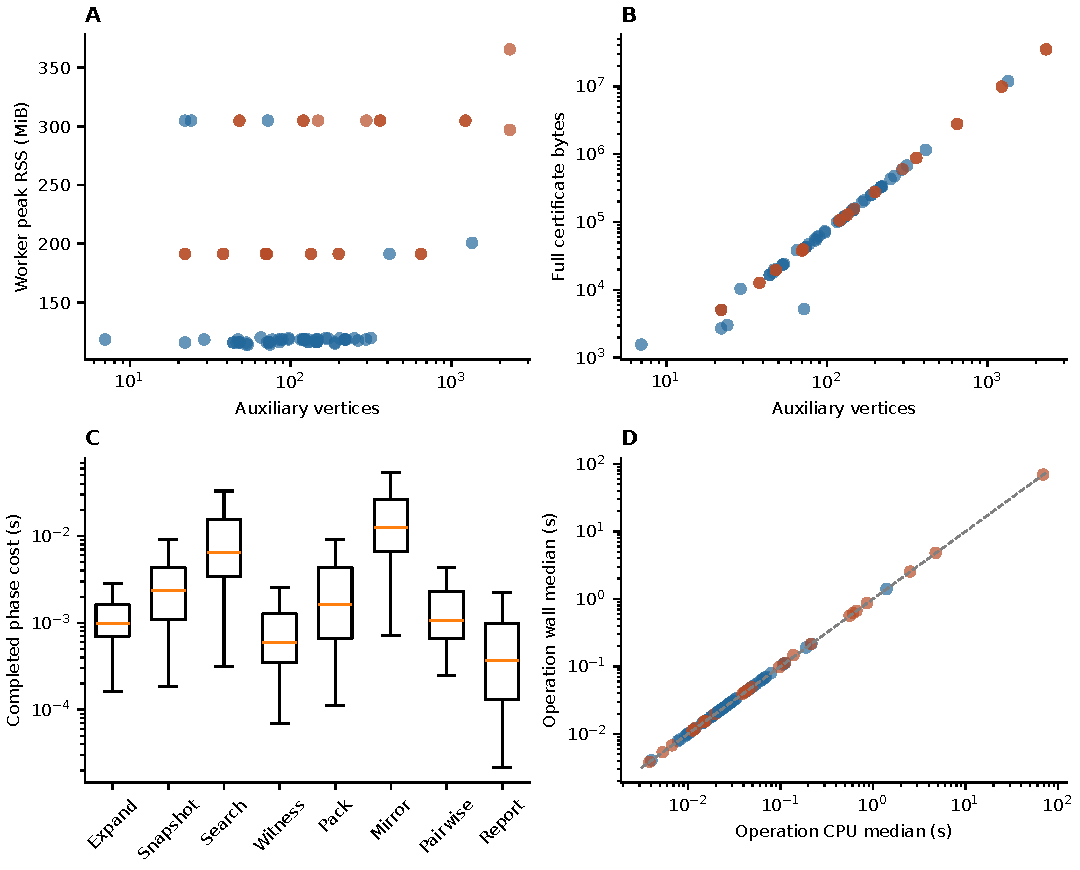
\includegraphics[width=0.98\textwidth]{fig/controlled_stereo_resources.pdf}
\caption{Completed generator-mode resource measurements. (A) Median native
worker peak RSS, including interpreter and imported libraries. (B) Full
certificate size. (C) Per-trial phase distributions; boxes give quartiles,
whiskers use the standard 1.5-interquartile-range rule and outliers are omitted
only from this panel. Pairwise timing covers its declared six-family subset;
report timing serializes the worker's measurement payload. (D) Operation CPU
versus wall medians, excluding interpreter startup. Blue denotes ordinary
cases and orange stress cases. Censored trials are absent from these panels
and retained in Table~\ref{tab:cost-coverage}.}
\label{fig:controlled-resources}
\end{figure*}

\begingroup
% The main-text six-shape gallery defines private drawing helpers with the
% same names as the denser appendix galleries. Replace them within this group.
\let\sqF\relax
\let\tbpF\relax
\let\octF\relax
\let\bondF\relax
% Shared local-frame drawers for the SI orbit galleries.
% \input in the preamble (after tikz + concept_style).  Each macro draws one
% coordination frame at (cx,cy); ligand identity is passed as fill colors in
% slot order.  Slot numbering is shown once per figure via a key, not per cell.
\providecolor{pballA}{RGB}{68,119,170}
\providecolor{pballB}{RGB}{238,119,51}
\providecolor{pballC}{RGB}{34,136,51}
\providecolor{pballD}{RGB}{170,51,119}
\providecolor{pballE}{RGB}{102,204,238}
\providecolor{pballF}{RGB}{221,204,68}

\tikzset{
  sball/.style={circle, draw=black!30, minimum size=3.7mm, inner sep=0pt},
  sbond/.style={line width=0.6pt, black!55, line cap=round},
  scen/.style={circle, draw=black!35, fill=black!45, minimum size=1.7mm,
               inner sep=0pt},
  scarb/.style={circle, draw=black!45, fill=white, minimum size=3.0mm,
                inner sep=0pt, font=\tiny},
  slab/.style={font=\tiny, text=black!70, inner sep=1pt},
  slotk/.style={font=\tiny, text=black!60, inner sep=0.4pt},
}

% specular highlight: turns a flat disc into a sphere (matches the main gallery)
\newcommand{\shl}[2]{%
  \fill[white,opacity=0.16] ({#1-0.056},{#2+0.056}) circle (0.056);}
% slot key drawn once per gallery: \slotkey{x}{y}{list of slot labels}
\newcommand{\slotkey}[3]{\node[slotk, anchor=west] at (#1,#2)
  {slots in frame order: #3};}

% square planar: center + 4 ligands N,E,S,W  (slots 1,2,3,4)
\newcommand{\sqF}[6]{\begin{scope}[shift={(#1,#2)}]
  \foreach \p in {(0,0.60),(0.60,0),(0,-0.60),(-0.60,0)} \draw[sbond] (0,0)--\p;
  \node[scen] at (0,0){};
  \node[sball,fill=#3] at (0,0.60){}; \node[sball,fill=#4] at (0.60,0){};
  \node[sball,fill=#5] at (0,-0.60){}; \node[sball,fill=#6] at (-0.60,0){};
  \shl{0}{0.60}\shl{0.60}{0}\shl{0}{-0.60}\shl{-0.60}{0}
\end{scope}}

% trigonal bipyramidal: center + 2 axial + 3 equatorial (slots 1,2 axial; 3,4,5 eq)
\newcommand{\tbpF}[7]{\begin{scope}[shift={(#1,#2)}]
  \foreach \p in {(0,0.72),(0,-0.72),(-0.66,0.05),(0.66,0.18),(0.52,-0.32)}
    \draw[sbond] (0,0)--\p;
  \node[scen] at (0,0){};
  \node[sball,fill=#3] at (0,0.72){}; \node[sball,fill=#4] at (0,-0.72){};
  \node[sball,fill=#5] at (-0.66,0.05){}; \node[sball,fill=#6] at (0.66,0.18){};
  \node[sball,fill=#7] at (0.52,-0.32){};
  \shl{0}{0.72}\shl{0}{-0.72}\shl{-0.66}{0.05}\shl{0.66}{0.18}\shl{0.52}{-0.32}
\end{scope}}

% octahedral: center + 4 equatorial (square) + 2 axial (slots 1-4 eq; 5,6 axial)
\newcommand{\octF}[8]{\begin{scope}[shift={(#1,#2)}]
  \foreach \p in {(-0.48,0.28),(0.48,0.28),(0.48,-0.28),(-0.48,-0.28),(0,0.74),(0,-0.74)}
    \draw[sbond] (0,0)--\p;
  \node[scen] at (0,0){};
  \node[sball,fill=#3] at (-0.48,0.28){}; \node[sball,fill=#4] at (0.48,0.28){};
  \node[sball,fill=#5] at (0.48,-0.28){}; \node[sball,fill=#6] at (-0.48,-0.28){};
  \node[sball,fill=#7] at (0,0.74){}; \node[sball,fill=#8] at (0,-0.74){};
  \shl{-0.48}{0.28}\shl{0.48}{0.28}\shl{0.48}{-0.28}\shl{-0.48}{-0.28}%
  \shl{0}{0.74}\shl{0}{-0.74}
\end{scope}}

% bond frame: two centers + 2 substituents each end.  #7=1 double / 0 single.
% colors are left-top, left-bottom, right-top, right-bottom (slots 1,2,5,6).
\newcommand{\bondF}[7]{\begin{scope}[shift={(#1,#2)}]
  \coordinate (cL) at (-0.34,0); \coordinate (cR) at (0.34,0);
  \ifnum#7=1
    \draw[sbond] (-0.34,0.05)--(0.34,0.05); \draw[sbond] (-0.34,-0.05)--(0.34,-0.05);
  \else
    \draw[sbond] (cL)--(cR);
  \fi
  \draw[sbond] (cL)--(-0.82,0.44); \draw[sbond] (cL)--(-0.82,-0.44);
  \draw[sbond] (cR)--(0.82,0.44);  \draw[sbond] (cR)--(0.82,-0.44);
  \node[scarb] at (cL){}; \node[scarb] at (cR){};
  \node[sball,fill=#3] at (-0.82,0.44){}; \node[sball,fill=#4] at (-0.82,-0.44){};
  \node[sball,fill=#5] at (0.82,0.44){};  \node[sball,fill=#6] at (0.82,-0.44){};
  \shl{-0.82}{0.44}\shl{-0.82}{-0.44}\shl{0.82}{0.44}\shl{0.82}{-0.44}
\end{scope}}


\section{Scope and claim boundary of the technical appendices}
\label{sec:si-scope}

These appendices consolidate the technical contracts for the
molecular-graph layer of \synkit's configuration-neutral stereochemical
identity model: carrier perception and constitutional evidence, typed supports,
frames, groups, orbits, relation classes, witnesses,
stereo-preserving morphisms, graph identity, derived-label projection, and
whole-molecule chirality. Reaction-layer operations, including rule guards and
effects, reference-aligned stereo change, reversal, imaginary transition
states and mechanism replay, are outside the present validation scope.

The novelty boundary is explicit.  Ordered local frames modulo finite geometry
groups are prior M{\O}D work, while permutation-invariant local descriptors and
whole-graph stereoisomer comparison are also provided by \stereomolgraph
\cite{andersen2017stereo,papusha2026stereomolgraph}.  This work does not claim
either premise as new.  Its claim is the evidence-bearing contract joining
configuration-neutral chemical-neighbourhood frames and carrier-stabilizer tie
certificates to typed configured states, double-coset relations, composable
transport witnesses, exact global equivalence, and derived labels that cannot
feed back into identity.  The complete configured object is additionally
encoded as a coloured auxiliary stereograph whose exact canonical label is the
exact configured-stereograph identity certificate.

The SACA comparison uses its accessible primary abstract and the authors'
inspected experiment source, rather than attributing guarantees from an
unavailable full text \cite{papusha2026saca}. Its resonance-invariant circular
fingerprints are credited separately from the full-certificate identity
contract studied here.

The method is compatible with the ordered-local-frame and finite-group
model used by M{\O}D; it is not claimed to be a complete
monomorphic Double-Pushout implementation, a three-dimensional perception
engine, or a predictor of stereochemical outcome.

Eight orbit shapes are registered---tetrahedral, square-planar,
trigonal-bipyramidal, octahedral, planar-bond, atrop-axis, cumulene-axis,
and extended-cis/trans---together with configured helical-path and planar-chirality
descriptors.  Global support is implemented by the coupled-frame
\code{FrameworkStereo} descriptor and an orientation-unspecified analysis
certificate.  Section~\ref{sec:si-classsets} states exactly which consumers
accept which classes.

\section{Reproducibility and environment manifest}
\label{sec:si-manifest}

\begingroup
\small
\renewcommand{\code}[1]{\path{#1}}
\begin{table}[htbp]
\caption{Research artifacts and their provenance.}
\label{tab:manifest}
\centering
\begin{tabularx}{\textwidth}{@{}lXX@{}}
\toprule
Artifact & Recorded revision & Retained evidence \\
\midrule
\synkit source & Package metadata \code{1.6.2}; clean experiment commit \code{e2526b9} & Exact source and input hashes; complete raw execution archive \\
Core fixtures & \code{Test/Graph/Stereo}, \code{Test/Graph/Morphism}, \code{Test/Chem/Molecule} & Frozen cases and source checksums in the research archive \\
Recorded environment & Linux, Python 3.12.12; 46-package base and separate comparator overlay & Wheel-hash locks and original conda bootstrap specification \\
Optional comparator & Current \stereomolgraph \code{2b99f62}; historical \code{2189f61} remains separate & Pinned comparison reports and MIT notice; no runtime dependency \\
Benchmark registry & \code{Experiment/Stereo/Data/manifest.json}, schema \code{synkit.stereo-benchmark-registry/1} & Dataset revisions, input hashes, attribution and separate source licences \\
\bottomrule
\end{tabularx}
\end{table}
\endgroup

Descriptor equality, finite group actions, support projection, morphism
construction, CIP ranking, and label projection are deterministic and use no
random seed.  Stereoisomer enumeration for the chirality benchmark is capped
and the cap is reported with the result.

\section{Typed supports}
\label{sec:si-supports}

Support answers where a stereo element lives.  It deliberately does not encode
configuration, CIP labels, provenance, or configurational stability.

\begin{table}[htbp]
\caption{Support families, their data, and their validation invariants.}
\label{tab:supports}
\centering
\begin{tabularx}{\textwidth}{@{}lXX@{}}
\toprule
Family & Data & Rejects \\
\midrule
Atom & one centre & non-integer centre \\
Bond & two endpoints & equal endpoints \\
Axis & ordered path of \(\ge 2\) atoms; two ordered two-reference terminal
frames & repeated path atoms; wrong frame count or width; duplicate references
inside one terminal frame \\
Path & ordered atoms; open/cyclic flag & fewer than two atoms; repeated atoms;
cyclic with fewer than three atoms \\
Plane & \(\ge 3\) oriented atoms & fewer than three atoms; repeated atoms \\
Global & component atom set & empty or non-integer atom set \\
\bottomrule
\end{tabularx}
\end{table}

Every support exposes a dependency set---the atoms whose renumbering affects
it---and a relabelling action.  Axis-support relabelling covers the path, the
material references in both terminal frames, and the owners of virtual
references, so that \code{@H:<owner>} and \code{@LP:<owner>} follow their atom.

\section{Permutation-orbit data model}

\subsection{Frames, groups, and canonical identity}

A permutation \(p\) acts by
\[
 p(N)_i=N_{p(i)},
\]
and \code{p.then(q)} has slot image \(p\circ q\), so
\code{p.then(q).apply(N)} equals \code{q.apply(p.apply(N))}.
Atom-supported frames place the
locus first and then their ligand references.  Bond- and axis-supported frames
use \((l_1,l_2,l,r,r_1,r_2)\).  Material references are atom maps; virtual
ligands have the owner-scoped forms \code{@H:<owner>} and
\code{@LP:<owner>}.

For a registered shape \(\tau\) with geometry group \(\Gamma_\tau\) and frame
\(N\), a fixed configuration is the orbit \([N]_{\Gamma_\tau}\), and the number
of configurations is the index \([\Sigma_\tau:\Gamma_\tau]\) of
Proposition~\ref{prop:config-count}.  The canonical representative is
the minimum deterministically encoded orbit member.  Two configurations are
equal exactly when shape, specification level, and canonical frame agree.

\begin{table}[htbp]
\caption{Registered fixed and unspecified group actions.}
\label{tab:groups}
\centering
\begin{tabularx}{\textwidth}{@{}llXX@{}}
\toprule
Shape & Support & Fixed group & Unspecified information group \\
\midrule
Tetrahedral & atom & \(A_4\), order 12 & \(S_4\), order 24 \\
Square planar & atom & \(D_4\), order 8 & \(S_4\), order 24 \\
Trigonal bipyramidal & atom & \(D_3\), order 6 & \(S_5\), order 120 \\
Octahedral & atom & proper \(O\), order 24 & \(S_6\), order 720 \\
Planar bond & bond & \(V_4\), order 4 & bond-frame group, order 8 \\
Atrop axis & axis & \(V_4\), order 4 & bond-frame group, order 8 \\
Cumulene axis & axis & \(V_4\), order 4 & bond-frame group, order 8 \\
\bottomrule
\end{tabularx}
\end{table}

Planar-bond, atrop-axis, and cumulene-axis fixed actions are distinct even
though all three are abstractly \(V_4\): they differ in their frame-reversal
action and in the support that may carry them.  Stored unspecified orientation
uses the larger group and is distinct from descriptor absence and query
wildcard behavior.  The legacy
\code{atoms}, \code{parity}, and \code{provenance} fields remain compatible
encodings; parity is decoded to a concrete frame and is not mathematical
identity.  Existing \code{canonical\_form()} and serialized descriptor payloads
remain the Beta-2 compatibility boundary, and \code{AtropBondStereo} remains a
wire-compatible alias of \code{AtropAxisStereo}.

\subsection{Permutation orbits of the six atom- and bond-supported geometries}
\label{sec:si-orbits}

The tetrahedral orbit structure is drawn exhaustively in the main text: all
\(4!=24\) orderings of four distinguishable ligands split into two
\(12\)-element orbits (the even rotations \(A_4\) and their odd mirror images),
so a stored descriptor is the orbit, in practice the parity.
Figures~\ref{fig:si-square}--\ref{fig:si-atrop} apply the same construction to
the remaining five geometries, using the same colour-for-ligand convention;
each cell is one frame ordering, labelled by the permutation that produces it
from the reference in cycle notation over the numbered slots.  All cells,
groupings, and labels were generated directly from the registered groups of
Table~\ref{tab:groups}.  Where the full ordering set is too large to draw
(trigonal-bipyramidal, \(5!=120\); octahedral, \(6!=720\)), one
configuration's orbit---the frame maps belonging to \(\Gamma_\tau\)---is shown
and the total configuration count \([\Sigma_\tau:\Gamma_\tau]\) is stated.
The cumulene-axis frame is not drawn: its group and orbit structure coincide
with the atrop frame of Figure~\ref{fig:si-atrop}, and it differs in support
and admissibility rather than in group action.

\begin{figure*}[htbp]
  \centering
  \resizebox{0.72\textwidth}{!}{\begin{tikzpicture}[font=\small,
  blkc/.style={rounded corners=4pt, draw=black!18, fill=black!2, line width=0.4pt}]
\draw[blkc] (-1.70,1.45) rectangle (8.75,-3.80);
\draw[blkc] (-1.70,-4.05) rectangle (8.75,-9.30);
\draw[blkc] (-1.70,-9.55) rectangle (8.75,-14.80);
\node[iocbadge] at (-1.45,1.02){A};
\node[slab,anchor=west,font=\footnotesize,text=black!75] at (-1.05,1.02){configuration 1 ($8$ equivalent orderings)};
\sqF{0.00}{0.00}{pballA}{pballB}{pballC}{pballD}
\node[slab] at (0.00,-0.98){$\mathrm{id}$};
\sqF{2.40}{0.00}{pballA}{pballD}{pballC}{pballB}
\node[slab] at (2.40,-0.98){$(2\,4)$};
\sqF{4.80}{0.00}{pballB}{pballA}{pballD}{pballC}
\node[slab] at (4.80,-0.98){$(1\,2)(3\,4)$};
\sqF{7.20}{0.00}{pballB}{pballC}{pballD}{pballA}
\node[slab] at (7.20,-0.98){$(1\,2\,3\,4)$};
\sqF{0.00}{-2.35}{pballC}{pballB}{pballA}{pballD}
\node[slab] at (0.00,-3.33){$(1\,3)$};
\sqF{2.40}{-2.35}{pballC}{pballD}{pballA}{pballB}
\node[slab] at (2.40,-3.33){$(1\,3)(2\,4)$};
\sqF{4.80}{-2.35}{pballD}{pballA}{pballB}{pballC}
\node[slab] at (4.80,-3.33){$(1\,4\,3\,2)$};
\sqF{7.20}{-2.35}{pballD}{pballC}{pballB}{pballA}
\node[slab] at (7.20,-3.33){$(1\,4)(2\,3)$};
\node[iocbadge] at (-1.45,-4.48){B};
\node[slab,anchor=west,font=\footnotesize,text=black!75] at (-1.05,-4.48){configuration 2 ($8$ equivalent orderings)};
\sqF{0.00}{-5.50}{pballA}{pballB}{pballD}{pballC}
\node[slab] at (0.00,-6.48){$(3\,4)$};
\sqF{2.40}{-5.50}{pballA}{pballC}{pballD}{pballB}
\node[slab] at (2.40,-6.48){$(2\,3\,4)$};
\sqF{4.80}{-5.50}{pballB}{pballA}{pballC}{pballD}
\node[slab] at (4.80,-6.48){$(1\,2)$};
\sqF{7.20}{-5.50}{pballB}{pballD}{pballC}{pballA}
\node[slab] at (7.20,-6.48){$(1\,2\,4)$};
\sqF{0.00}{-7.85}{pballC}{pballA}{pballB}{pballD}
\node[slab] at (0.00,-8.83){$(1\,3\,2)$};
\sqF{2.40}{-7.85}{pballC}{pballD}{pballB}{pballA}
\node[slab] at (2.40,-8.83){$(1\,3\,2\,4)$};
\sqF{4.80}{-7.85}{pballD}{pballB}{pballA}{pballC}
\node[slab] at (4.80,-8.83){$(1\,4\,3)$};
\sqF{7.20}{-7.85}{pballD}{pballC}{pballA}{pballB}
\node[slab] at (7.20,-8.83){$(1\,4\,2\,3)$};
\node[iocbadge] at (-1.45,-9.98){C};
\node[slab,anchor=west,font=\footnotesize,text=black!75] at (-1.05,-9.98){configuration 3 ($8$ equivalent orderings)};
\sqF{0.00}{-11.00}{pballA}{pballC}{pballB}{pballD}
\node[slab] at (0.00,-11.98){$(2\,3)$};
\sqF{2.40}{-11.00}{pballA}{pballD}{pballB}{pballC}
\node[slab] at (2.40,-11.98){$(2\,4\,3)$};
\sqF{4.80}{-11.00}{pballB}{pballC}{pballA}{pballD}
\node[slab] at (4.80,-11.98){$(1\,2\,3)$};
\sqF{7.20}{-11.00}{pballB}{pballD}{pballA}{pballC}
\node[slab] at (7.20,-11.98){$(1\,2\,4\,3)$};
\sqF{0.00}{-13.35}{pballC}{pballA}{pballD}{pballB}
\node[slab] at (0.00,-14.33){$(1\,3\,4\,2)$};
\sqF{2.40}{-13.35}{pballC}{pballB}{pballD}{pballA}
\node[slab] at (2.40,-14.33){$(1\,3\,4)$};
\sqF{4.80}{-13.35}{pballD}{pballA}{pballC}{pballB}
\node[slab] at (4.80,-14.33){$(1\,4\,2)$};
\sqF{7.20}{-13.35}{pballD}{pballB}{pballC}{pballA}
\node[slab] at (7.20,-14.33){$(1\,4)$};
\node[slotk,anchor=west] at (-1.55,-15.15){slots: $1$ N, $2$ E, $3$ S, $4$ W};
\end{tikzpicture}
}
  \caption{Square planar.  All \(24\) orderings of four distinct ligands,
  grouped by configuration.  Here \(\Sigma_\tau=S_4\) and
  \(\Gamma_\tau=D_4\) of order \(8\), so each configuration is an orbit of
  \(8\) orderings and there are \([\Sigma_\tau:\Gamma_\tau]=24/8=3\)
  configurations; unlike the tetrahedral case there is no single binary
  ``opposite'', which is why nonidentity square-planar relations are general
  \code{RECONFIGURED} classes.}
  \label{fig:si-square}
\end{figure*}

\begin{figure}[htbp]
  \centering
  \resizebox{0.62\columnwidth}{!}{\begin{tikzpicture}[font=\small,
  blkc/.style={rounded corners=4pt, draw=black!18, fill=black!2, line width=0.4pt}]
\draw[blkc] (-1.70,1.75) rectangle (6.55,-3.80);
\node[iocbadge] at (-1.45,1.32){A};
\node[slab,anchor=west,font=\footnotesize,text=black!75] at (-1.05,1.32){one configuration: the $|\Gamma_\tau|=6$ preserving maps};
\tbpF{0.00}{0.00}{pballA}{pballB}{pballC}{pballD}{pballE}
\node[slab] at (0.00,-0.98){$\mathrm{id}$};
\tbpF{2.40}{0.00}{pballB}{pballA}{pballD}{pballC}{pballE}
\node[slab] at (2.40,-0.98){$(1\,2)(3\,4)$};
\tbpF{4.80}{0.00}{pballB}{pballA}{pballE}{pballD}{pballC}
\node[slab] at (4.80,-0.98){$(1\,2)(3\,5)$};
\tbpF{0.00}{-2.35}{pballB}{pballA}{pballC}{pballE}{pballD}
\node[slab] at (0.00,-3.33){$(1\,2)(4\,5)$};
\tbpF{2.40}{-2.35}{pballA}{pballB}{pballD}{pballE}{pballC}
\node[slab] at (2.40,-3.33){$(3\,4\,5)$};
\tbpF{4.80}{-2.35}{pballA}{pballB}{pballE}{pballC}{pballD}
\node[slab] at (4.80,-3.33){$(3\,5\,4)$};
\node[slotk,anchor=west] at (-1.55,-4.15){slots $1,2$ axial; $3,4,5$ equatorial};
\end{tikzpicture}
}
  \caption{Trigonal bipyramidal.  The six orderings forming one configuration
  (the \(\Gamma_\tau=D_3\) orbit: an axial pair and an equatorial triple).
  With five distinct ligands there are
  \([\Sigma_\tau:\Gamma_\tau]=120/6=20\) configurations in total, so only one
  \(6\)-element orbit is drawn.}
  \label{fig:si-tbp}
\end{figure}

\begin{figure*}[htbp]
  \centering
  \resizebox{\textwidth}{!}{\begin{tikzpicture}[font=\small,
  blkc/.style={rounded corners=4pt, draw=black!18, fill=black!2, line width=0.4pt}]
\draw[blkc] (-1.70,1.75) rectangle (13.15,-8.50);
\node[iocbadge] at (-1.45,1.32){A};
\node[slab,anchor=west,font=\footnotesize,text=black!75] at (-1.05,1.32){one configuration: the $|\Gamma_\tau|=24$ preserving maps};
\octF{0.00}{0.00}{pballA}{pballB}{pballC}{pballD}{pballE}{pballF}
\node[slab] at (0.00,-0.98){$\mathrm{id}$};
\octF{2.40}{0.00}{pballB}{pballA}{pballD}{pballC}{pballF}{pballE}
\node[slab] at (2.40,-0.98){$(1\,2)(3\,4)(5\,6)$};
\octF{4.80}{0.00}{pballB}{pballA}{pballE}{pballD}{pballC}{pballF}
\node[slab] at (4.80,-0.98){$(1\,2)(3\,5)$};
\octF{7.20}{0.00}{pballB}{pballA}{pballF}{pballE}{pballD}{pballC}
\node[slab] at (7.20,-0.98){$(1\,2)(3\,6)(4\,5)$};
\octF{9.60}{0.00}{pballB}{pballA}{pballC}{pballF}{pballE}{pballD}
\node[slab] at (9.60,-0.98){$(1\,2)(4\,6)$};
\octF{12.00}{0.00}{pballC}{pballE}{pballA}{pballF}{pballB}{pballD}
\node[slab] at (12.00,-0.98){$(1\,3)(2\,5)(4\,6)$};
\octF{0.00}{-2.35}{pballC}{pballE}{pballB}{pballD}{pballA}{pballF}
\node[slab] at (0.00,-3.33){$(1\,3\,2\,5)$};
\octF{2.40}{-2.35}{pballC}{pballE}{pballD}{pballA}{pballF}{pballB}
\node[slab] at (2.40,-3.33){$(1\,3\,4)(2\,5\,6)$};
\octF{4.80}{-2.35}{pballC}{pballE}{pballF}{pballB}{pballD}{pballA}
\node[slab] at (4.80,-3.33){$(1\,3\,6)(2\,5\,4)$};
\octF{7.20}{-2.35}{pballD}{pballF}{pballE}{pballA}{pballC}{pballB}
\node[slab] at (7.20,-3.33){$(1\,4)(2\,6)(3\,5)$};
\octF{9.60}{-2.35}{pballD}{pballF}{pballC}{pballB}{pballE}{pballA}
\node[slab] at (9.60,-3.33){$(1\,4\,2\,6)$};
\octF{12.00}{-2.35}{pballD}{pballF}{pballA}{pballC}{pballB}{pballE}
\node[slab] at (12.00,-3.33){$(1\,4\,3)(2\,6\,5)$};
\octF{0.00}{-4.70}{pballD}{pballF}{pballB}{pballE}{pballA}{pballC}
\node[slab] at (0.00,-5.68){$(1\,4\,5)(2\,6\,3)$};
\octF{2.40}{-4.70}{pballE}{pballC}{pballB}{pballF}{pballA}{pballD}
\node[slab] at (2.40,-5.68){$(1\,5)(2\,3)(4\,6)$};
\octF{4.80}{-4.70}{pballE}{pballC}{pballA}{pballD}{pballB}{pballF}
\node[slab] at (4.80,-5.68){$(1\,5\,2\,3)$};
\octF{7.20}{-4.70}{pballE}{pballC}{pballF}{pballA}{pballD}{pballB}
\node[slab] at (7.20,-5.68){$(1\,5\,4)(2\,3\,6)$};
\octF{9.60}{-4.70}{pballE}{pballC}{pballD}{pballB}{pballF}{pballA}
\node[slab] at (9.60,-5.68){$(1\,5\,6)(2\,3\,4)$};
\octF{12.00}{-4.70}{pballF}{pballD}{pballE}{pballB}{pballC}{pballA}
\node[slab] at (12.00,-5.68){$(1\,6)(2\,4)(3\,5)$};
\octF{0.00}{-7.05}{pballF}{pballD}{pballC}{pballA}{pballE}{pballB}
\node[slab] at (0.00,-8.03){$(1\,6\,2\,4)$};
\octF{2.40}{-7.05}{pballF}{pballD}{pballA}{pballE}{pballB}{pballC}
\node[slab] at (2.40,-8.03){$(1\,6\,3)(2\,4\,5)$};
\octF{4.80}{-7.05}{pballF}{pballD}{pballB}{pballC}{pballA}{pballE}
\node[slab] at (4.80,-8.03){$(1\,6\,5)(2\,4\,3)$};
\octF{7.20}{-7.05}{pballA}{pballB}{pballD}{pballE}{pballF}{pballC}
\node[slab] at (7.20,-8.03){$(3\,4\,5\,6)$};
\octF{9.60}{-7.05}{pballA}{pballB}{pballE}{pballF}{pballC}{pballD}
\node[slab] at (9.60,-8.03){$(3\,5)(4\,6)$};
\octF{12.00}{-7.05}{pballA}{pballB}{pballF}{pballC}{pballD}{pballE}
\node[slab] at (12.00,-8.03){$(3\,6\,5\,4)$};
\node[slotk,anchor=west] at (-1.55,-8.85){slots $1$--$4$ equatorial; $5,6$ axial};
\end{tikzpicture}
}
  \caption{Octahedral.  The \(24\) orderings forming one configuration (the
  proper rotation group \(\Gamma_\tau=O\)).  With six distinct ligands there
  are \([\Sigma_\tau:\Gamma_\tau]=720/24=30\) configurations in total (the
  classical \([Mabcdef]\) stereoisomer count); only one \(24\)-element orbit is
  drawn.}
  \label{fig:si-oct}
\end{figure*}

\begin{figure*}[htbp]
  \centering
  \resizebox{0.78\textwidth}{!}{\begin{tikzpicture}[font=\small,
  blkc/.style={rounded corners=4pt, draw=black!18, fill=black!2, line width=0.4pt}]
\draw[blkc] (-1.90,1.35) rectangle (10.00,-1.85);
\draw[blkc] (-1.90,-1.85) rectangle (10.00,-5.05);
\node[iocbadge] at (-1.65,0.95){A};
\node[slab,anchor=west,font=\footnotesize,text=black!75] at (-1.25,0.95){configuration 1 ($E$)};
\bondF{0.00}{-0.65}{pballA}{pballB}{pballC}{pballD}{1}
\node[slab] at (0.00,-1.63){$\mathrm{id}$};
\bondF{2.65}{-0.65}{pballB}{pballA}{pballD}{pballC}{1}
\node[slab] at (2.65,-1.63){$(1\,2)(5\,6)$};
\bondF{5.30}{-0.65}{pballC}{pballD}{pballA}{pballB}{1}
\node[slab] at (5.30,-1.63){$(1\,5)(2\,6)(3\,4)$};
\bondF{7.95}{-0.65}{pballD}{pballC}{pballB}{pballA}{1}
\node[slab] at (7.95,-1.63){$(1\,6)(2\,5)(3\,4)$};
\node[iocbadge] at (-1.65,-2.25){B};
\node[slab,anchor=west,font=\footnotesize,text=black!75] at (-1.25,-2.25){configuration 2 ($Z$)};
\bondF{0.00}{-3.85}{pballB}{pballA}{pballC}{pballD}{1}
\node[slab] at (0.00,-4.83){$\mathrm{id}$};
\bondF{2.65}{-3.85}{pballA}{pballB}{pballD}{pballC}{1}
\node[slab] at (2.65,-4.83){$(1\,2)(5\,6)$};
\bondF{5.30}{-3.85}{pballC}{pballD}{pballB}{pballA}{1}
\node[slab] at (5.30,-4.83){$(1\,5)(2\,6)(3\,4)$};
\bondF{7.95}{-3.85}{pballD}{pballC}{pballA}{pballB}{1}
\node[slab] at (7.95,-4.83){$(1\,6)(2\,5)(3\,4)$};
\node[slotk,anchor=west] at (-1.75,-5.40){slots $1,2$ left end; $5,6$ right end};
\end{tikzpicture}
}
  \caption{Planar bond (\(E/Z\)).  The eight bond-frame maps split into two
  orbits of four; each orbit is one configuration.  Here
  \(\Gamma_\tau=V_4\) of order \(4\) sits inside the bond-frame group
  \(\Sigma_\tau\) of order \(8\), so \([\Sigma_\tau:\Gamma_\tau]=2\) and a
  single admissible one-end swap realizes the binary
  \(E\!\leftrightarrow\!Z\) opposite of Corollary~\ref{cor:binary-opposite}.}
  \label{fig:si-planar}
\end{figure*}

\begin{figure*}[htbp]
  \centering
  \resizebox{0.78\textwidth}{!}{\begin{tikzpicture}[font=\small,
  blkc/.style={rounded corners=4pt, draw=black!18, fill=black!2, line width=0.4pt}]
\draw[blkc] (-1.90,1.35) rectangle (10.00,-1.85);
\draw[blkc] (-1.90,-1.85) rectangle (10.00,-5.05);
\node[iocbadge] at (-1.65,0.95){A};
\node[slab,anchor=west,font=\footnotesize,text=black!75] at (-1.25,0.95){configuration 1 ($P$)};
\bondF{0.00}{-0.65}{pballA}{pballB}{pballC}{pballD}{0}
\node[slab] at (0.00,-1.63){$\mathrm{id}$};
\bondF{2.65}{-0.65}{pballB}{pballA}{pballD}{pballC}{0}
\node[slab] at (2.65,-1.63){$(1\,2)(5\,6)$};
\bondF{5.30}{-0.65}{pballC}{pballD}{pballB}{pballA}{0}
\node[slab] at (5.30,-1.63){$(1\,5\,2\,6)(3\,4)$};
\bondF{7.95}{-0.65}{pballD}{pballC}{pballA}{pballB}{0}
\node[slab] at (7.95,-1.63){$(1\,6\,2\,5)(3\,4)$};
\node[iocbadge] at (-1.65,-2.25){B};
\node[slab,anchor=west,font=\footnotesize,text=black!75] at (-1.25,-2.25){configuration 2 ($M$)};
\bondF{0.00}{-3.85}{pballB}{pballA}{pballC}{pballD}{0}
\node[slab] at (0.00,-4.83){$\mathrm{id}$};
\bondF{2.65}{-3.85}{pballA}{pballB}{pballD}{pballC}{0}
\node[slab] at (2.65,-4.83){$(1\,2)(5\,6)$};
\bondF{5.30}{-3.85}{pballC}{pballD}{pballA}{pballB}{0}
\node[slab] at (5.30,-4.83){$(1\,5\,2\,6)(3\,4)$};
\bondF{7.95}{-3.85}{pballD}{pballC}{pballB}{pballA}{0}
\node[slab] at (7.95,-4.83){$(1\,6\,2\,5)(3\,4)$};
\node[slotk,anchor=west] at (-1.75,-5.40){slots $1,2$ left end; $5,6$ right end};
\end{tikzpicture}
}
  \caption{Atrop axis.  The eight frame maps split into two orbits
  of four; each orbit is one assigned axial sense.  Again
  \(\Gamma_\tau=V_4\leq\Sigma_\tau\) with \([\Sigma_\tau:\Gamma_\tau]=2\),
  realizing the binary \(P\!\leftrightarrow\!M\) opposite; unlike the planar
  bond, the improper extension here also has index two, which is why the axis
  is chiral.  The frame
  is drawn with a single bond to distinguish it from the planar-bond
  ($\pi$-bearing) frame of Figure~\ref{fig:si-planar}.  The cumulene-axis frame
  shares this structure over an even-cumulene path.}
  \label{fig:si-atrop}
\end{figure*}

\subsection{Relations and witnesses}

If a concrete permutation \(\pi\) transports one fixed frame to another, the
representative-independent relation class is the double coset
\(\Gamma_\tau\pi\Gamma_\tau\) of Lemma~\ref{lem:double-coset}.  \code{StereoRelation} stores a stable minimum class
identifier and a concrete \code{PermutationWitness}.  Witnesses compose;
double-coset identifiers do not.  The public relation kinds are
\code{EQUIVALENT}, \code{OPPOSITE}, \code{RECONFIGURED},
\code{UNRELATED}, and \code{UNSPECIFIED}.

Only tetrahedral, planar-bond, atrop-axis, and cumulene-axis shapes declare a
binary opposite.  Nonidentity square-planar, trigonal-bipyramidal, and
octahedral relations are general reconfigurations.  This is why a
non-tetrahedral legacy \code{INVERTED} label can coexist with authoritative
\code{reconfigured:<class>} evidence.

\section{Extended descriptors without a finite frame group}

\subsection{Cumulene axes}

A cumulene-axis descriptor stores the full ordered axis path and two ordered
two-reference terminal frames owned by the first and last path atoms.
Validation requires at least three path atoms, pairwise distinct path atoms,
integer path entries, exactly two terminal frames of width two, references
distinct within each frame, and an \emph{even} number of cumulated bonds.  The
even-bond requirement is the classical parity rule: an even run places the
terminal substituent planes orthogonally and the element is axis-supported and
chiral, whereas an odd run places them coplanar and the element is the
bond-supported \(E/Z\) case.

\subsection{Helical paths}

A helical descriptor stores an ordered path of at least four atoms, an
open/cyclic flag, a parity in \(\{-1,+1\}\) or \(\bot\), optional reported
positions lying on the path, and an optional non-empty coupling identity.
Identity is the canonical path form: for an open path, the minimum of the path
and its reversal; for a cyclic path, the minimum over all rotations of the path
and of its reversal.  Equality compares descriptor class, canonical path,
cyclicity, parity, and coupling identity.

Reported positions associate several reported atoms with one configuration and
do not create independent local stereocentres; they are emitted in canonical
path order.  A fixed helical configuration may be constructed only through an
authorized evidence source, and the declared-sidecar constructor requires an
explicit \code{evidence\_source} marker on deserialization, so bare
connectivity cannot produce one.  Reference replacement is refused on path
atoms, which protects the locus in the same way that locus positions are
protected in frame-based descriptors.

\subsection{Descriptor-class sets}
\label{sec:si-classsets}

\begin{table}[htbp]
\caption{Descriptor-class sets and the consumers that accept them.}
\label{tab:classsets}
\centering
\begin{tabularx}{\textwidth}{@{}lXl@{}}
\toprule
Set & Members & Size \\
\midrule
Legacy supported set (prefilter/rule consumers) & tetrahedral, square-planar,
trigonal-bipyramidal, octahedral, planar-bond, atrop & 6 \\
Local configured (exact certificate) & supported set, plus
cumulene-axis, extended cis/trans, helical, and planar chirality & 10 \\
Coupled framework (exact certificate/mirror) & fixed framework orientation
with relative frame coupling; helper enumeration/focal operations refuse & 1 \\
Local enumeration and focal evidence & the ten local configured families;
framework inputs deliberately refuse & 10 \\
Descriptor JSON restoration & all local configured families and framework & 11 \\
\rdkit{} adapter & the supported set & 6 \\
Deferred (declared names only) & \code{rigid\_bond\_33}, \code{rigid\_bond\_23},
\code{rigid\_bond\_13}, \code{rigid\_bond\_12} & 4 \\
\bottomrule
\end{tabularx}
\end{table}

\subsection{Exact auxiliary stereograph}

For each configured registry, the exact encoder creates typed vertices for
atoms, bonds, stereo loci, owner-specific ligand ports, virtual resources,
allowed orbit tuples, and position-coloured tuple slots.  Constitution and
stereo are therefore canonicalized together by the native exact coloured-graph
kernel.  The certificate schema is
\code{synkit.canonical-stereograph/2}.  Equality compares complete canonical
graphs; the associated SHA-256 digest is an index, not a substitute proof.

The pairwise classifier first compares constitution-only certificates.  Equal
constitutions are then compared as configured stereographs and, if unequal,
after geometry-specific mirror transformation of the left registry.  The
outcomes are \code{IDENTICAL}, \code{ENANTIOMERS}, \code{DIASTEREOMERS},
\code{CONSTITUTIONALLY\_DIFFERENT}, \code{INCOMPLETE}, and
\code{UNSUPPORTED}, and \code{INFORMATION\_MISMATCH}. RDKit drawing keys
record their selected profile under \code{synkit.rdkit-stereograph/1}; chemical
family keys use \code{synkit.resonance-family-stereograph/1}. Canonicalization
and pairwise operations retain their Lewis-state defaults, while mirror
assessment defaults to chemical family identity. Select a common explicit
profile when comparing these operations. The pairwise result schema is
\code{synkit.stereoisomer-relation/2}.

\section{Proof-bearing computational entities}
\label{sec:si-entities}

\begingroup
\small
\renewcommand{\code}[1]{\path{#1}}
\begin{longtable}{@{}p{0.30\textwidth}p{0.63\textwidth}@{}}
\caption{Public molecular-layer value objects and evidence contracts.}\label{tab:objects}\\
\toprule
Object & Contract \\
\midrule
\endfirsthead
\toprule
Object & Contract \\
\midrule
\endhead
\code{StereoSupport} family & Immutable typed carrier with dependency set and relabelling that commutes with descriptor relabelling \\
\code{PotentialStereoElement} & Candidate carrier type, typed support, supplied-configuration state, provenance, and source identifier; no stereogenicity or configuration claim \\
\code{TetrahedralConstitution} & Center-fixed exact ligand orbits, multiplicities, automorphism count, and constitutionally-distinct or symmetry-related status \\
\code{StereoConfiguration} & Shape, specification level, concrete and canonical frames, relation and replacement operations \\
\code{HelicalStereo} & Path support, cyclicity, parity, reported positions, coupling identity, canonical path form \\
\code{PermutationWitness} & Concrete position permutation whose replay is checked \\
\code{StereoRelation} & Kind, double-coset class, and replayable witness \\
\code{GraphMorphism} & Immutable total injective material-node embedding with typed wildcard environment \\
\code{StereoMorphism} & Graph morphism plus local stereo certificates and explicit policy choices \\
\code{LocalStereoCertificate} & Layer, endpoint configurations, relation, witness, effective policy, and matched/ignored/propagate status \\
\code{CIPRanking} & Ordered references, per-pair comparisons, completeness flag, and digest \\
\code{CIPAssignment} & Label or typed status, rankings, supplemental comparisons, projection witness, required rules, and digest \\
\code{MolecularChirality\-Result} & Classification, mirror isomorphism witness, descriptor counts, and evidence provenance \\
\bottomrule
\end{longtable}
\endgroup

\subsection{Stereo-preserving graph morphisms}

\code{StereoMorphism} proves match compatibility; it does not classify a
reaction-induced change. Material references are transported through the
underlying injective map.  Virtual hydrogen and lone-pair tokens retain their
typed owner.  A mapped explicit hydrogen removed by normalization is projected
onto virtual H only when owner-local evidence makes the projection unique.

Every matched local certificate is checked twice: its witness must replay the
transported frame, and its stored relation kind and class must agree with direct
endpoint classification.  Missing references, invalid virtual owners,
non-injective maps, missing required targets, strict target extras, and forged
witnesses are structured failures.

\begin{table}[htbp]
\caption{Independent stereo-morphism policy axes.}
\label{tab:policies}
\centering
\begin{tabularx}{\textwidth}{@{}llX@{}}
\toprule
Axis & Value & Meaning \\
\midrule
Information & \code{exact} & Fixed matches equivalent fixed; unspecified matches unspecified \\
Information & \code{wildcard} & An unspecified query may specialize; a fixed query remains exact \\
Information & \code{either} & As wildcard; a fixed query may also use its declared compatibility alternative \\
Presence & \code{require} & Every source descriptor has one valid target; target extras allowed \\
Presence & \code{strict} & Require, and reject unmatched target descriptors touching the image \\
Presence & \code{ignore} & Accept structurally and emit explicit ignored certificates \\
Presence & \code{propagate} & Emit a visible obligation for a source descriptor without a target \\
\bottomrule
\end{tabularx}
\end{table}

Identity stereo morphisms contain identity node maps and witnesses.  Composition
pairs the concrete intermediate configurations, composes witnesses, replays the
composition on the transported source, and reclassifies the direct endpoint
relation.  The canonical signature includes shape, information level, status,
policy, class, witness permutation, virtual-reference kinds, and wildcard-frame
positions, and is invariant under consistent endpoint renumbering.

\subsection{Value identity and hashing}

For stereo-bearing graphs the map-invariant registry form built from
connectivity/LLG colour-refinement tokens is a prefilter only.
Equality enumerates exact structural isomorphisms and accepts one only if every
registered descriptor aligns into its fixed group.  Equal objects hash equally;
equal hashes are never reported as isomorphism.

\section{Derived-label projection}
\label{sec:si-cip}

\subsection{Ranking kernel}

Ligand ranking is computed from molecular constitution, isotopes,
multiple-bond duplicate nodes, and ring closures.  No toolkit CIP code or rank
property is read.  Per-ligand evidence records, for each sphere, the node's
atomic number, mass, atom index, path, duplicate flag, duplicate source depth,
and duplicate kind, together with one of three termination reasons:
\code{exhausted}, \code{virtual\_reference}, or \code{depth\_cap}.

Rules are applied hierarchically: Rule~1a (atomic number, including averaged
duplicate atomic numbers for simple non-fused even mancude rings) is exhausted
over successive spheres before Rule~1b (duplicate-node distance), which
precedes Rule~2 (isotopic mass).  Rule~3 and the reference-independent,
single-corresponding-pair subset of Rules~4c/5 are active.  Each comparison
records its outcome
(\code{left\_higher}, \code{right\_higher}, \code{tie}, or
\code{unsupported}), the first deciding rule, the deciding depth, and the
compared witnesses on both sides.  Multi-unit reference-descriptor pairing
under Rule~4b and sequence-rule cases outside the implemented subset fail
closed.

\subsection{Assignment statuses}

\begin{table}[htbp]
\caption{Label-assignment statuses and their meaning.}
\label{tab:cipstatus}
\centering
\begin{tabularx}{\textwidth}{@{}lX@{}}
\toprule
Status & Meaning \\
\midrule
\code{assigned} & A label is justified by a complete ranking and a witnessed projection \\
\code{unspecified\_configuration} & The descriptor carries no orientation; no label may be emitted \\
\code{unresolved\_priority} & The ranking returned a tie at the required depth \\
\code{unsupported\_sequence\_rule} & The comparison requires an unimplemented sequence-rule case, notably multi-unit Rule~4b \\
\code{unsupported\_descriptor} & No CIP-style projection is claimed for this class (coordination geometries) \\
\bottomrule
\end{tabularx}
\end{table}

Axial \(M/P\) projection uses the IUPAC helicity convention from a witnessed
viewing direction.  When constitution cannot witness a stable viewing
direction---a symmetric axis---the projection fails closed rather than using
atom indices as a tiebreak.  Assignments are immutable reports: they never
mutate a molecule or descriptor, and their labels are absent from stereo
identity, hashing, rule matching, and descriptor serialization.

\section{Whole-molecule chirality}
\label{sec:si-chirality}

Classification searches for a stereo-preserving isomorphism between the
stereo-bearing graph and its descriptor-inverted mirror, refined by
connectivity and LLG colours and by semantic feasibility on
descriptors.  A verdict of achiral returns the mirror map as its witness.

For underspecified input the outcome is four-valued:
\code{necessarily\_achiral}, \code{necessarily\_chiral},
\code{configuration\_dependent}, and \code{unsupported\_or\_incomplete}.
Configuration dependence means at least one enumerated completion is chiral and
at least one is achiral; it is a definitive property of the constitution.
Enumeration is capped, mixed populations may terminate only after both classes
have been witnessed, and caps without an independent proof fail closed to
\code{unsupported\_or\_incomplete}.  For an oversized all-tetrahedral
assignment product, the implementation enumerates the constitutional
automorphisms instead.  Transport into the descriptor-inverted mirror gives
binary XOR constraints on the local configurations.  A satisfying assignment
is verified as an achiral witness; exhaustion of the automorphisms proves that
no achiral completion exists.

Detection of a potential stereo locus from two-dimensional connectivity yields
a typed \code{PotentialStereoLocus} carrying its axis support, an unspecified
orientation state, its evidence provenance, and an unassessed stability status.
Promotion to a fixed configuration requires an authorized evidence source:
\code{explicit\_stereo}, \code{validated\_geometry}, or
\code{declared\_sidecar}.  Molecular configuration evidence additionally
carries a stability state (\code{unassessed} or \code{validated}) and an
optional population fraction in \((0,1]\), kept distinct from orientation.

Broad tetrahedral-carrier detection precedes stereogenicity.  A carrier has
four represented or hidden-hydrogen slots but may have repeated ligands.  The
constitution-only canonicalizer uniquely marks the center, enumerates exact
attributed-graph automorphisms, and intersects their node orbits with the four
ligand slots.  Four singleton classes give
\code{constitutionally\_distinct}; any repeated class gives
\code{symmetry\_related}.  The latter is deliberately not called achiral,
because it means only that the configuration-neutral detector cannot confirm
the center.  Supplied configuration and CIP properties are not inputs and may
not split or reorder the constitutional neighbor classes.

\section{Finite propositions and executable obligations}

Let \(\tau\) be a registered shape, \(\Gamma_\tau\leq\Sigma_\tau\) its finite
geometry group inside the frame symmetry group, and \([N]\) the orbit of a
frame \(N\).

\paragraph{P0---Configuration-neutral frame construction.}
A local-frame constructor reads only constitutional attributes and is required
to commute with attributed-graph relabelling.  Exact support-stabilizer orbits
are its tie authority.  Conjugation transports the stabilizer and its reference
orbits under every graph isomorphism, proving that the tie certificate is
independent of atom numbering, supplied configuration, and CIP.  The executable
tetrahedral slice currently validates the orbit partition; recursive total
ordering of distinguishable classes is a subsequent implementation gate.

\paragraph{P1---Orbit canonicalization.}
The minimum of the deterministically ordered orbit is unique, and two fixed
configurations have the same canonical frame exactly when their frames share
one orbit.  Exhaustive atom-frame partitions contain 2, 3, 20, and 30 fixed
orbits for tetrahedral, square-planar, trigonal-bipyramidal, and octahedral
geometry; the bond and axis actions are also completely enumerated.

\paragraph{P2---Relabelling equivariance.}
For bijective relabelling \(f\), \([N]=[M]\) if and only if
\([f(N)]=[f(M)]\), because position actions commute with value relabelling
(Lemma~\ref{lem:frame-action}).

\paragraph{P3---Replacement well-definedness.}
An injective replacement of non-locus references that preserves frame
distinctness descends to orbit classes.  Missing sources, locus replacement,
and reference collisions are rejected.

\paragraph{P4---Relation invariance.}
The double coset \(\Gamma_\tau\pi\Gamma_\tau\) is unchanged when either endpoint is replaced
by an equivalent representative; relation kind and class ID are therefore
representative independent.  This is Lemma~\ref{lem:double-coset}, and the
gate checks it exhaustively for every registered action.

\paragraph{P5---Witness composition.}
If \(p\) replays \(A\to B\) and \(q\) replays \(B\to C\), then
\code{p.then(q)} replays \(A\to C\); the global form of this law is the cocycle
identity of Eq.~\eqref{eq:alignment-cocycle}.  Composition of stereo morphisms records
and rechecks both legs and the direct endpoint claim; the companion paper
extends the same obligation to reaction and fusion legs.

\paragraph{P6---Binary-opposite involution.}
For tetrahedral, planar-bond, atrop-axis, and cumulene-axis shapes,
\(\operatorname{opp}(\operatorname{opp}([N]))=[N]\).  These are exactly the
index-two families of Corollary~\ref{cor:binary-opposite}, which also shows why
the three coordination geometries are not forced into a binary relation.

\paragraph{P7---Support commutation.}
For every configured descriptor \(d\) and relabelling \(f\),
\(\operatorname{support}(\operatorname{relabel}(d,f))
 =\operatorname{relabel}(\operatorname{support}(d),f)\).
Axis-support relabelling covers path atoms, material terminal references, and
virtual-reference owners.

\paragraph{P8---Axis laws.}
Every preserving terminal order and axis reversal yields an equivalent
configuration; axis reversal and mirror action are involutions; an unspecified
axis forgets terminal order but not its path; and reference replacement is
refused on the full locus.

\paragraph{P9---Path laws.}
Open-path reversal, and cyclic rotation together with reversal, are
identity-preserving and involutive; mirror inversion changes only a fixed
helical configuration; relabelling commutes with path support and
canonicalization; reported positions are one coupled configuration rather than
independent local centres; and coupling identity distinguishes two
configurations on the same path.

\paragraph{P10---No inference from bare connectivity.}
Two-dimensional topology detection produces only potential loci.  Identical
supports may carry opposite configurations only when an authorized evidence
source declares them.

\paragraph{P11---Label independence.}
Ranking is invariant under atom renumbering and fragment order; labels are
invariant under renumbering, fragment order, valid support reversal, and
descriptor canonicalization; mirror inversion changes the label exactly where
the specification requires; toolkit CIP properties are never inputs; and no
label is emitted from an unspecified configuration.

\paragraph{P12---Complete certificate invariance.}
For every configured family, relabelling atoms and reconstructing the complete
auxiliary stereograph preserves the exact certificate
(Corollary~\ref{cor:numbering-independence}); changing a fixed
configuration changes it unless a whole-graph automorphism identifies the two
states.  CIP cache properties never enter vertex colours.

\paragraph{P13---Whole-stereograph relation partition.}
After constitution equality is established, direct certificate equality,
left-mirror equality, and residual inequality partition complete same-
constitution pairs into identical, enantiomeric, and diastereomeric outcomes.
Missing configuration and unsupported population semantics remain
nondefinitive.

\begingroup
\small
\renewcommand{\code}[1]{\path{#1}}
\begin{longtable}{@{}p{0.08\textwidth}p{0.85\textwidth}@{}}
\caption{Principal executable obligations.}\label{tab:obligations}\\
\toprule
Claim & Principal test \\
\midrule
\endfirsthead
\toprule
Claim & Principal test \\
\midrule
\endhead
P1 & \code{Test/Graph/Stereo/test_orbit_kernel.py::test_all_atom_frame_permutations_partition_into_expected_fixed_orbits} and the bond-frame orbit-size test \\
P2--P3 & \code{test_relabeling_and_reference_replacement_are_equivariant} plus descriptor-migration locus protection \\
P4 & \code{test_relation_class_is_independent_of_fixed_representatives} \\
P5 & \code{test_witness_composition_replays_direct_transport} \\
P6 & \code{test_binary_opposite_is_an_involution} \\
P7 & \code{Test/Graph/Stereo/test_support_hierarchy.py::test_existing_descriptors_expose_typed_support_without_wire_changes} and \code{test_axis_support_relabeling_includes_path_material_and_virtual_owners} \\
P8 & \code{Test/Graph/Stereo/test_axis_descriptors.py::test_every_preserving_terminal_order_and_axis_reversal_is_equivalent} and \code{test_axis_reversal_and_mirror_actions_are_involutions} \\
P9 & \code{Test/Graph/Stereo/test_helical_descriptors.py::test_open_path_reversal_is_identity_preserving_and_involutive}, \code{test_cyclic_rotation_and_reversal_are_identity_preserving}, and \code{test_reported_positions_are_one_coupled_configuration_not_local_centers} \\
P10 & \code{test_connectivity_detection_still_returns_only_potential_support} and \code{test_bare_connectivity_does_not_infer_helicity} \\
P11 & \code{Test/Chem/Molecule/test_cip_ranking.py::test_atom_renumbering_preserves_the_rank_order}, \code{test_toolkit_cip_properties_are_not_inputs_to_ranking}, and \code{Test/Chem/Molecule/test_cip_assignment.py::test_atom_renumbering_and_fragment_order_preserve_the_label} \\
P12 & \code{Test/Graph/Stereo/test_configured_stereograph_families.py} and \code{test_canonical_stereograph_determinism.py}; public exhaustive relabelling report \code{exact_canonicalization_report.json} \\
P13 & \code{Test/Graph/Stereo/test_pairwise_stereoisomer_relations.py} and \code{stereoisomer_relation_report.json} \\
\bottomrule
\end{longtable}
\endgroup

\section{Validation corpus and conformance}

Deterministic fixtures cover the registered shapes, the extended axis and path
descriptors, support validation, symmetric isomorphisms, query policies,
morphism policy axes, composition, CIP ranking and assignment, and
serialization of descriptor payloads.

\begin{table}[htbp]
\caption{Development-snapshot conformance results for the molecular-graph
layer.}
\label{tab:results}
\centering
\begin{tabularx}{\textwidth}{@{}lXX@{}}
\toprule
Gate & Result & Boundary \\
\midrule
Full Pytest suite & 3881 passed; 6 skipped; 179 passing subtests & Repository snapshot, 2026-07-26 \\
Orbit, support, axis, path, and plane laws & Exhaustive enumeration for all registered actions; P7--P12 fixtures pass & Algebraic method boundaries \\
All-family local quotient & 940 raw representations yield 67/67 expected classes & Ten configured families \\
All-family exact certificates & 67/67 classes distinct within family; 0 collision or timeout & Every configured class \\
Configuration-free local corpus & 66,468/66,468 representations; 3,476/3,476 carriers & 1,218 Internal, ACS, CIP, and RotA rows \\
Formal mixed-family A/B/C & 2,160/2,160 assignments; 30/30 cases; 38/95/752 classes & Simultaneous carrier configurations; no failure or timeout \\
Raw mixed-family A/B/C slice & 3,353,600/3,353,600 encodings over 22 scoped cases & Complete A and B plus complete VS146 slice of C; no failure or timeout \\
Synthetic whole-graph relabelling & 201 per-class plus 528 representative checks; 0 failures & Exhaustive \(5!\) for four small fixtures, sampled otherwise \\
Mirror closure & 67/67 classes closed; 7 fixed & Three square-planar, two planar-bond, plus two extended-cis/trans classes \\
Public ACS certificate audit & 888/888 atom permutations invariant; 4/4 CIP-cache removals invariant & Four small configured records \\
Multi-element composition & 32 assignments yield 31 classes; 13 enantiomer and 64 diastereomer pairs & Six designed graphs; every class mirrored \\
Multi-element ACS audit & 14/14 sampled renumberings; 7/7 mirror labels & Seven records with 18 configured elements \\
Pairwise relation matrix & 9/9 correct & P13 designed conformance cases \\
\bottomrule
\end{tabularx}
\end{table}

The configuration-free local totals comprise 6,999 theoretical local classes
and 5,885 observed whole-graph classes.  The difference of 1,114 is fully
accounted for by exact global-symmetry quotients.  Formal A, B, and C contain
48, 192, and 1,920 assignments, respectively.  Raw A independently enumerates
all 2,048 local encodings and produces the same 48 formal tuples and 38 global
classes as formal A.  The larger raw runs are stress evidence rather than
additional assumptions of the correctness theorem.  Raw B enumerates all
992,256 encodings and recovers
the same 192 formal tuples and 95 classes as formal B.  The raw C/VS146 stress
run enumerates all 2,359,296 encodings for that record and recovers its 64
formal tuples and 64 classes.  The other eight C raw products are deliberately
absent from the maintained reproduction command; formal C nevertheless
exhausts all nine cases by Corollary~\ref{cor:raw-formal-global}.

The optional \stereomolgraph bridge uses direct descriptor exchange.  A legacy
molecule-reconstruction diagnostic is retained only to show why bond-order
recovery by another toolkit is not an appropriate acceptance criterion.
\stereomolgraph remains absent from runtime dependencies.  The pre-split
300/300 bridge and 6/6 conformance totals are not current evidence and must be
regenerated before inclusion in the submission artifact.

\section{Frozen chemical annotation and replay}
\label{sec:chemical-annotation}

The source-selection manifests record retrieval, terms, exact checksums,
constitution keys and annotation conventions. The coordination and negative
selections are outside the ACS/CIP/RotA development constitutions. The RotA
sample is explicitly drawn from that development data. Original annotations
remain archived byte-unchanged. The clean-release replay regenerates annotations
and production reports, binds their SHA-256 checksums, and reproduces every
scientific summary field. The manuscript summary recomputes its counts from
those four fresh reports; their execution provenance is separately recorded.
Selection, annotation, production evaluation and mathematical reference
coverage therefore remain separate audit steps.

For coordination, the first source conformer is used without selecting the
best later conformer. Donor-slot isotope labels are removed before assigning
the physical constitutional profile, while the supplied local tetrahedral
annotations are transported into the reference and production inputs.
The independent octahedral fit minimizes normalized RMSD over proper
rotations and all donor-slot assignments. Its acceptance limits were fixed
before evaluation: normalized RMSD at most 0.35 and a gap of at least 0.02
to the next inequivalent pose. The same criteria apply to the reflected
coordinates. The two refusals are \code{Mn\_PNhP\_iPr\_tri\_0} and
\code{Ru\_NNhN\_iPr\_tri\_0}, with RMSDs approximately 0.490 and 0.489.
They remain in the selected denominator and are not recast as incorrect
production predictions. The \ChemicalCoordinationCertified{} certified
examples retain \ChemicalCoordinationRetainedTetrahedralFrames{} local frames;
their independent source/mirror relations are
\ChemicalCoordinationSourceAchiral{} achiral and
\ChemicalCoordinationSourceChiral{} chiral. These are configured-graph
relations under the declared retained information.

Direct reference enumeration covers all
\ChemicalCoordinationReferenceAssignments{} formal assignments. Production
replays every reference partition and mirror map, then compares the
certificates of certified source, source-renumbered, coordinate-mirrored and
production-mirrored states. The resulting equality relation must neither split
one reference class nor merge different classes. The
\ChemicalCoordinationObservedSourceMirrorClasses{} observed classes are
therefore a subset of the \ChemicalCoordinationReferenceClasses{} reference
classes, rather than a claimed evaluation of every generated reference pose.

The sourced biaryl negatives are retained with original retrieval responses
and failed-query exclusions. Their truth witnesses preserve the complete
typed graph, fix the two axis endpoints, and exchange a declared terminal
ligand pair. The same map is replayed before original/renumbered perception.
This checks a constitutional counterexample to axis confirmation; it neither
estimates a kinetic barrier nor labels a compound experimentally achiral.

The RotA annotation contains every frozen sample locus and records uncertainty
without replacing difficult cases. Of \ChemicalRotAAxisSupports{} axis
supports, \ChemicalRotATerminalRelatedAxes{} admit the terminal-exchange
witness and \ChemicalRotATerminalConfirmedAxes{} exhaust the bounded search
without one. This terminal criterion differs from global configured identity:
a simultaneous exchange at both ends can preserve a coupled axis orientation.
The complete per-case assignments, partitions, mirror involutions and
transport composition checks define the reference used in the production
comparison. For atom pairs and spiro categories, geometry does not by itself
confirm the focal tetrahedral support. Negative tetrahedral perception may
omit a symmetry-related center, and the category projection requires the
actual focal carrier status. All \ChemicalRotAPerceptionComputations{}
original/renumbered perception comparisons are checked against those frozen
expectations. The \ChemicalRotASumPerCaseClasses{} reported classes are
summed over cases and are not a count of distinct chemical compounds.
Experimental persistence remains unknown throughout this sample.

\section{Local perception and naming benchmarks}

\begin{table}[htbp]
\caption{Task-specific two-setting local validation.  ``Retained'' uses
supplied orientation only at other local-neighbor frames; ``erased'' removes
all configuration.  CIP positions and labels are not global chirality truth;
RotA is positive-only.}
\label{tab:si-local}
\centering
\begin{tabularx}{\textwidth}{@{}XrrrX@{}}
\toprule
Task & Retained & Erased & Reference & Additional evidence \\
\midrule
ACS configured source loci & \AcsRetainedRecovered & \AcsErasedRecovered & \AcsErasedReferenceLoci & \AcsRetainedAdditional/\AcsErasedAdditional{} additional candidates \\
CIP all local positions & \CipRetainedRecovered & \CipErasedRecovered & \CipErasedReferenceLoci & \CipRetainedAdditional/\CipErasedAdditional{} additional candidates \\
\quad tetrahedral & \CipTetrahedralRetainedRecovered & \CipTetrahedralErasedRecovered & \CipTetrahedralErasedReference & Exact center-stabilizer criterion \\
\quad planar & \CipPlanarRetainedRecovered & \CipPlanarErasedRecovered & \CipPlanarErasedReference & Typed planar carriers \\
\quad axial/helical & \CipAxialRetainedRecovered & \CipAxialErasedRecovered & \CipAxialErasedReference & No stability claim \\
RotA annotated typed loci & \RotARetainedRecovered & \RotAErasedRecovered & \RotAErasedReferenceLoci & \RotAErasedAdditional{} broad additional projections \\
RotA expanded cumulene paths & \RotAExpandedRetainedRecovered & \RotAExpandedErasedRecovered & \RotAExpandedErasedReference & Modulo path reversal \\
Reverse-renumbered records & \DevelopmentRows & \DevelopmentRows & \DevelopmentRows & Complete invariance in each setting \\
CIP coordinate-assisted exact records & \multicolumn{2}{c}{\CipCoordinatesExactRecords} &
\CipCoordinatesRecords & \CipCoordinatesCorrectLabels/\CipCoordinatesExpectedLabels{} labels;
\CipCoordinatesEmittedLabels{} emitted \\
\bottomrule
\end{tabularx}
\end{table}

All \DevelopmentRows{} records are invariant under reverse atom renumbering independently
in both settings. The erased setting misses \AcsErasedMisses{} ACS and \CipErasedMisses{} CIP positions;
all \AllErasedMisses{} are carbon tetrahedral carriers classified as symmetry-related by the
configuration-erased center stabilizer and all are recovered in the retained
setting. ACS contains \AcsAcyclicMisses{} acyclic and \AcsRingMisses{} ring misses; CIP contains \CipAcyclicMisses{}
acyclic and \CipRingMisses{} ring misses. Available neighbor evidence comprises \AllTetrahedralNeighborMisses{}
tetrahedral-only, \AllPlanarNeighborMisses{} planar-only, \AllMixedNeighborMisses{} mixed tetrahedral--planar, and \CipCumuleneNeighborMisses{}
cumulene case.

Additional candidates are serialized per record.  Their retained/erased
counts are \AcsRetainedAdditional/\AcsErasedAdditional{} for ACS and \CipRetainedAdditional/\CipErasedAdditional{} for CIP. RotA has \RotAErasedAdditional{} additional
broad typed projections in either setting. Restricting to constitutionally
confirmed carriers recovers \RotAConfirmedRecovered/\RotAReferenceLoci{}
annotated loci and leaves \RotAConfirmedAdditional{} additional projections.
Confirmed spiro-category projections require actual confirmed tetrahedral
supports; geometry alone does not supply confirmation. These values are annotation-list
differences, not false-positive rates: ACS local annotations are incomplete
and RotA is positive-only.  They make no handedness, configurational-stability,
or whole-molecule chirality claim.

A separate synthetic negative protocol contains \SyntheticAxisNegatives{} constitutional controls.
\SyntheticAxisWitnessNegatives{} axis-like cases have exact axis-fixed automorphisms exchanging a
terminal ligand pair, and \SyntheticAxisNoSupportNegatives{} have no supported axis topology. Every case
is invariant under reverse atom renumbering and the confirmed-axis
false-positive count is zero.  Because these are constitutional proofs rather
than kinetic measurements, they do not validate rotational barriers,
isolation timescales, stability, or handedness.

\paragraph{CIP source versions.}
The provided publisher supporting archive (DOI
\url{https://doi.org/10.1021/acs.jcim.8b00324.s001}) is unchanged and is
licensed under CC~BY-NC~4.0. Preparation repairs citation punctuation in
VS297 and VS298 only; all 300 molecular inputs and expected labels are
unchanged, and the resulting SMILES file matches the evaluated checksum.
The original publisher SDF differs from the later GitHub SDF at VS095
(atom ordering and conformer) and in those two citation fields.
Original and amended coordinates have separate accepted checksums. A fresh
full 300-record evaluation of the original SDF reproduces every native naming
record and every RDKit comparator record from the amended-SDF evaluation;
the primary numerical manifest now identifies that original-source report.
This agreement does not assert coordinate equivalence. The publisher grant
is asserted only for the
provided original data and documented citation repair.

The pinned-coordinate CIP naming protocol has 73.96\% micro-label recall and
98.83\% precision; the SMILES-only exact-record baseline remains 175/300.
The 113 non-exact records are retained as 83 ranking defects, 21 missing-
orientation cases, and 9 unsupported classes.  Rules 1a/1b/2, simple
mancude-ring averaging, Rule 3, and the reference-independent one-pair subset
of Rules 4c/5 are active; multi-unit Rule 4b remains fail-closed.
The input-contract audit also identifies a strict information boundary:
VS010 and VS011 have the same supplied SMILES but opposite helical labels, so
SMILES-only exact-record accuracy is bounded by \CipSmilesDeterministicCeiling/\CipSmilesRecords. In the pinned
3D file, atom positions 1--4 have opposite nonzero signed normalized
volumes for the two records.  This translation- and proper-rotation-invariant,
reflection-sensitive witness makes the pair distinguishable without reading
its reference labels. The coordinate protocol completes both helical records,
all five CT4 records, four of seven AT records, and the fully material-framed
VS144 cumulene; the remaining sequence rules and extended classes remain
incomplete.

\section{Whole-molecule chirality benchmark}

\begin{table}[htbp]
\caption{Supplied-stereo protocol on the 258-record ACS validation set.
Comparator columns are the publisher's recorded results.  ``Agreement'' is
cross-profile agreement with the ACS topology labels, not internal certificate
correctness.  ACS labels: 94 achiral, 164 chiral.}
\label{tab:si-chirality}
\centering
\begin{tabularx}{\textwidth}{@{}Xrr@{}}
\toprule
Procedure & Agreement & Fraction \\
\midrule
Topology completion (this work) & 258/258 & 1.000 \\
Exact + necessary global certificate & 257/258 & 0.996 \\
\stereomolgraph (published) & 258/258 & 1.000 \\
InChI (published) & 238/258 & 0.922 \\
\rdkit{} SMILES (published) & 235/258 & 0.911 \\
chython (published) & 210/258 & 0.814 \\
Exact supplied stereograph & \AcsSourceCorrect/\AcsSourceRecords & 0.981 \\
\bottomrule
\end{tabularx}
\end{table}

The exact-stereograph row is a separate 5\,s per-case supplied-configuration audit.
It preserves every explicit source \code{@}/\code{@@} atom configuration and
leaves additional undeclared potential loci unconstrained. Chemical identity
compares the exact resonance family while retaining genuine bond-order
differences. It gives \AcsSourceDefinitive{} definitive outcomes, of which
\AcsSourceCorrect{} agree, and times out on VS126, VS127 and VS208. VS170 is chiral
under chemical identity because
its \code{S-I} and \code{S\#I} ligands remain distinct, whereas the ACS topology profile
omits bond order. In VS300 the exact certificate mirror fixes the central
configured atom and exchanges the two configured cages; the ACS result instead
depends on global topology-completion probes outside the configured support
catalogue.
This audit makes no configured-locus completeness claim and must not be
presented as the source of the topology-completion 258/258 result.

The separately versioned exact-plus-global protocol uses a 30-second budget
for source-declared identity and adds a map-independent, orientation-unspecified
coupled-frame certificate.  It proves VS300 necessarily chiral and therefore
agrees with 257/258 ACS labels.  It does not choose a VS300 enantiomer and does
not alter the frozen source-declared report; VS170 remains a declared chemical
identity/profile difference.

\begin{table}[htbp]
\caption{Stereo-stripped four-state protocol on the same set, 256-isomer cap.
The 258 records reduce to 214 unique constitutions.}
\label{tab:si-fourstate}
\centering
\begin{tabularx}{\textwidth}{@{}Xr@{}}
\toprule
Outcome & Rows \\
\midrule
Necessarily chiral & 125 \\
Necessarily achiral & 66 \\
Configuration dependent & 67 \\
Unsupported or incomplete & 0 \\
\midrule
Definitive rows & 258 \\
Erased manual label still in the possible population & 258 \\
\bottomrule
\end{tabularx}
\end{table}

Coverage asks whether the erased manual label remains among the possible
configurations; it is not recovery accuracy, because the input configuration was
deliberately destroyed.  VS226 exhausts after six symmetry-unique isomers and
is necessarily achiral.  Exact automorphism-parity analysis proves VS265 and
VS266 necessarily chiral and supplies both class witnesses for
configuration-dependent VS268, without enumerating their multi-million-entry
raw assignment spaces.

The RotA and CIP datasets are not scored as chirality benchmarks.  Historical
binary columns for those datasets used an exploratory arbitrary-axis
orientation and carry a machine-readable retraction; they must not be cited as
current classification or accuracy.

\section{Reproduction commands}

\begin{verbatim}
# from repository root in the locked Linux/Python 3.12 environment
PYTHON=python bash scripts/lint.sh
PYTHON=python bash scripts/pytest.sh -q Test/
python -m Experiment.Stereo.reproduce --tier bounded --jobs 2 \
  --output-dir /tmp/stereo-bounded
python -m Experiment.Stereo.reproduce --tier full --jobs 2 \
  --stereomolgraph /path/to/pinned/StereoMolGraph \
  --output-dir /tmp/stereo-full

# compile this paper
cd paper/stereo_graph
latexmk -pdf main.tex
\end{verbatim}

The release instructions specify the wheel-hash environment lock, the separate
optional-comparator dependency overlay and exact comparator commit. The
complete 35-stage clean execution retains every report and stage log. Optional
raw Cartesian stress is excluded from this sequence and remains separately
identified historical supplemental evidence.

\section{Known limitations}

\begin{itemize}
  \item The local descriptors do not infer coordinates, conformations,
        configurational stability, reaction selectivity, or preferred paths.
  \item Planar chirality and coupled tetrahedral framework orientation are
        configured. Additional global geometry families and configured
        orientation perception remain unsupported. The analyzer fails closed
        above 256 support atoms or 64 coupled frames and for disconnected
        frame-bearing components. The four
        \code{rigid\_bond} variants are class
        names only, and enhanced stereo groups remain deferred.
  \item The exact certificate consumes all ten configured classes.
        Cumulene-axis, helical, and planar-chiral descriptors remain outside
        the narrower legacy graph-identity, rule, JSON/GML, and \rdkit{}
        surfaces.
  \item Exact configured canonicalization currently materializes complete
        local orbits and uses verified automorphism pruning.  The retained ACS
        audit has no 2\,s timeout, but larger raw local products remain outside
        the maintained benchmark.
\item The RotA corpus is positive-only.  Full annotated-locus recovery therefore
      does not validate the 1,562 additional broad axis candidates, their
      configurational stability, or their handedness.  The 24 synthetic
      negatives validate constitutional specificity but not those experimental
      properties.
  \item RDKit round-trips the six supported classes and assigned
        non-tetrahedral/atrop states; unsupported unknown orientations fail
        explicitly.
  \item The CIP kernel implements Rules~1a, 1b, and 2, simple mancude-ring
        averaging, Rule~3, and the reference-independent one-pair subset of
        Rules~4c/5. Multi-unit Rule~4b and coordination-geometry projections
        remain fail-closed.  Full 300-record evaluation additionally requires
        coordinates or declared orientation evidence because two supplied
        SMILES are identical but configurationally opposite.
  \item Local finite-group evidence does not prove equivalence of \synkit's
        operational graph matching and a full DPO system.
\end{itemize}

\section{Attribution and reproducibility checklist}

The ordered local-list and group-action formulation follows Andersen, Flamm,
Merkle, and Stadler \cite{andersen2017stereo}.  The six-class relative
descriptor layer independently implements ideas from Papusha and Leonhard
\cite{papusha2026stereomolgraph}.  Non-tetrahedral tables were cross-validated against the MIT-licensed
\stereomolgraph commit named in Table~\ref{tab:manifest}; the retained notice is
\code{LICENSES/StereoMolGraph-MIT.txt}.  The CIP sequence-rule hierarchy
follows IUPAC recommendations P-92.  The ACS validation set is redistributed
under CC~BY-NC~4.0 and the RotA corpus under the MIT License. The original
CIP publisher inputs are included under CC~BY-NC~4.0 with attribution and
two explicitly documented bibliographic punctuation repairs.

The research archive retains the exact executed source and input checksums,
the environment lock, independent fixtures, unchanged raw execution reports
and the numerical manifest used to generate manuscript values. Package version,
source commit and report schema identify distinct parts of this provenance.
\endgroup

\end{document}
